\documentclass[]{book}
\usepackage{lmodern}
\usepackage{amssymb,amsmath}
\usepackage{ifxetex,ifluatex}
\usepackage{fixltx2e} % provides \textsubscript
\ifnum 0\ifxetex 1\fi\ifluatex 1\fi=0 % if pdftex
  \usepackage[T1]{fontenc}
  \usepackage[utf8]{inputenc}
\else % if luatex or xelatex
  \ifxetex
    \usepackage{mathspec}
  \else
    \usepackage{fontspec}
  \fi
  \defaultfontfeatures{Ligatures=TeX,Scale=MatchLowercase}
\fi
% use upquote if available, for straight quotes in verbatim environments
\IfFileExists{upquote.sty}{\usepackage{upquote}}{}
% use microtype if available
\IfFileExists{microtype.sty}{%
\usepackage{microtype}
\UseMicrotypeSet[protrusion]{basicmath} % disable protrusion for tt fonts
}{}
\usepackage[margin=1in]{geometry}
\usepackage{hyperref}
\hypersetup{unicode=true,
            pdftitle={Tesina Statistica},
            pdfauthor={Nicola Lancellotti},
            pdfborder={0 0 0},
            breaklinks=true}
\urlstyle{same}  % don't use monospace font for urls
\usepackage{natbib}
\bibliographystyle{apalike}
\usepackage{color}
\usepackage{fancyvrb}
\newcommand{\VerbBar}{|}
\newcommand{\VERB}{\Verb[commandchars=\\\{\}]}
\DefineVerbatimEnvironment{Highlighting}{Verbatim}{commandchars=\\\{\}}
% Add ',fontsize=\small' for more characters per line
\usepackage{framed}
\definecolor{shadecolor}{RGB}{248,248,248}
\newenvironment{Shaded}{\begin{snugshade}}{\end{snugshade}}
\newcommand{\KeywordTok}[1]{\textcolor[rgb]{0.13,0.29,0.53}{\textbf{#1}}}
\newcommand{\DataTypeTok}[1]{\textcolor[rgb]{0.13,0.29,0.53}{#1}}
\newcommand{\DecValTok}[1]{\textcolor[rgb]{0.00,0.00,0.81}{#1}}
\newcommand{\BaseNTok}[1]{\textcolor[rgb]{0.00,0.00,0.81}{#1}}
\newcommand{\FloatTok}[1]{\textcolor[rgb]{0.00,0.00,0.81}{#1}}
\newcommand{\ConstantTok}[1]{\textcolor[rgb]{0.00,0.00,0.00}{#1}}
\newcommand{\CharTok}[1]{\textcolor[rgb]{0.31,0.60,0.02}{#1}}
\newcommand{\SpecialCharTok}[1]{\textcolor[rgb]{0.00,0.00,0.00}{#1}}
\newcommand{\StringTok}[1]{\textcolor[rgb]{0.31,0.60,0.02}{#1}}
\newcommand{\VerbatimStringTok}[1]{\textcolor[rgb]{0.31,0.60,0.02}{#1}}
\newcommand{\SpecialStringTok}[1]{\textcolor[rgb]{0.31,0.60,0.02}{#1}}
\newcommand{\ImportTok}[1]{#1}
\newcommand{\CommentTok}[1]{\textcolor[rgb]{0.56,0.35,0.01}{\textit{#1}}}
\newcommand{\DocumentationTok}[1]{\textcolor[rgb]{0.56,0.35,0.01}{\textbf{\textit{#1}}}}
\newcommand{\AnnotationTok}[1]{\textcolor[rgb]{0.56,0.35,0.01}{\textbf{\textit{#1}}}}
\newcommand{\CommentVarTok}[1]{\textcolor[rgb]{0.56,0.35,0.01}{\textbf{\textit{#1}}}}
\newcommand{\OtherTok}[1]{\textcolor[rgb]{0.56,0.35,0.01}{#1}}
\newcommand{\FunctionTok}[1]{\textcolor[rgb]{0.00,0.00,0.00}{#1}}
\newcommand{\VariableTok}[1]{\textcolor[rgb]{0.00,0.00,0.00}{#1}}
\newcommand{\ControlFlowTok}[1]{\textcolor[rgb]{0.13,0.29,0.53}{\textbf{#1}}}
\newcommand{\OperatorTok}[1]{\textcolor[rgb]{0.81,0.36,0.00}{\textbf{#1}}}
\newcommand{\BuiltInTok}[1]{#1}
\newcommand{\ExtensionTok}[1]{#1}
\newcommand{\PreprocessorTok}[1]{\textcolor[rgb]{0.56,0.35,0.01}{\textit{#1}}}
\newcommand{\AttributeTok}[1]{\textcolor[rgb]{0.77,0.63,0.00}{#1}}
\newcommand{\RegionMarkerTok}[1]{#1}
\newcommand{\InformationTok}[1]{\textcolor[rgb]{0.56,0.35,0.01}{\textbf{\textit{#1}}}}
\newcommand{\WarningTok}[1]{\textcolor[rgb]{0.56,0.35,0.01}{\textbf{\textit{#1}}}}
\newcommand{\AlertTok}[1]{\textcolor[rgb]{0.94,0.16,0.16}{#1}}
\newcommand{\ErrorTok}[1]{\textcolor[rgb]{0.64,0.00,0.00}{\textbf{#1}}}
\newcommand{\NormalTok}[1]{#1}
\usepackage{longtable,booktabs}
\usepackage{graphicx,grffile}
\makeatletter
\def\maxwidth{\ifdim\Gin@nat@width>\linewidth\linewidth\else\Gin@nat@width\fi}
\def\maxheight{\ifdim\Gin@nat@height>\textheight\textheight\else\Gin@nat@height\fi}
\makeatother
% Scale images if necessary, so that they will not overflow the page
% margins by default, and it is still possible to overwrite the defaults
% using explicit options in \includegraphics[width, height, ...]{}
\setkeys{Gin}{width=\maxwidth,height=\maxheight,keepaspectratio}
\IfFileExists{parskip.sty}{%
\usepackage{parskip}
}{% else
\setlength{\parindent}{0pt}
\setlength{\parskip}{6pt plus 2pt minus 1pt}
}
\setlength{\emergencystretch}{3em}  % prevent overfull lines
\providecommand{\tightlist}{%
  \setlength{\itemsep}{0pt}\setlength{\parskip}{0pt}}
\setcounter{secnumdepth}{5}
% Redefines (sub)paragraphs to behave more like sections
\ifx\paragraph\undefined\else
\let\oldparagraph\paragraph
\renewcommand{\paragraph}[1]{\oldparagraph{#1}\mbox{}}
\fi
\ifx\subparagraph\undefined\else
\let\oldsubparagraph\subparagraph
\renewcommand{\subparagraph}[1]{\oldsubparagraph{#1}\mbox{}}
\fi

%%% Use protect on footnotes to avoid problems with footnotes in titles
\let\rmarkdownfootnote\footnote%
\def\footnote{\protect\rmarkdownfootnote}

%%% Change title format to be more compact
\usepackage{titling}

% Create subtitle command for use in maketitle
\newcommand{\subtitle}[1]{
  \posttitle{
    \begin{center}\large#1\end{center}
    }
}

\setlength{\droptitle}{-2em}

  \title{Tesina Statistica}
    \pretitle{\vspace{\droptitle}\centering\huge}
  \posttitle{\par}
    \author{Nicola Lancellotti}
    \preauthor{\centering\large\emph}
  \postauthor{\par}
      \predate{\centering\large\emph}
  \postdate{\par}
    \date{30/01/2019}

\usepackage[utf8]{inputenc}
\usepackage[italian]{babel}
\usepackage{booktabs}

\begin{document}
\maketitle

{
\setcounter{tocdepth}{1}
\tableofcontents
}
\chapter{Introduzione}\label{introduzione}

Lo scopo della presente tesina è quello di mettere in pratica le nozioni
teoriche apprese nel corso di ``Statistica e Analisi dei Dati''
\citep{sad} tenuto dalla professoressa Nobile all'Università degli Studi
di Salerno.

La prima parte, composta dai capitoli da 2 a 7, si occuperà della
statistica descrittiva, cioè la parte della statistica che si occupa
della rilevazione, analisi, sintesi, interpretazione e rappresentazione
dei dati di una popolazione o di una sua parte, detta campione.
L'oggetto di interesse su cui sarà applicata la statistica descrittiva è
la soddisfazione degli italiani per quanto riguarda la situazione
economica, di salute, delle relazioni con i membri della famiglia, delle
relazioni con gli amici e infine del proprio tempo libero. I dati sono
stati raccolti dall'ISTAT nel 2017 attraverso sondaggi su un campione
casuale. Il sondaggio consisteva nell'esprimere una valutazione
qualitativa per ognuna delle caratteristiche di interesse. I valori
qualitativi possibili erano: ``molto'', ``abbastanza'', ``poco'' e ``per
niente''. Infine è stata calcolata le percentuale di persone che hanno
espresso un voto pari a ``molto'' per ognuna delle caratteristiche e per
ognuna delle regioni italiane. Dopo una prima analisi visiva mediante i
boxplot verranno effettuate analisi numeriche volte a spiegare la
distribuzione del campione. Verranno quindi calcolate le frequenze e
verra analizzata la simmetria e la curtosi. In seguito verrano
analizzati gli indici di posizione e di dispersione. A seguire verranno
analizzate le correlazioni tra le caratteristiche del data set e infine
l'analisi dei cluster consentirà di scoprire le regioni simili tra loro
per quanto riguarda le caratteristiche analizzate.

La seconda parte, composta dai capitoli da 8 a 12, invece si occuperà
dell'inferenza statistica che ha lo scopo di estendere le misura
ricavate dal campione alla popolazione da cui il campione è stato
estratto. Verrà utilizzato un campione estratto da una popolazione
descritta da una distribuzione geometrica e verranno mostrate le
tecniche che consentono di stimare il parametro non noto \(p\) della
distribuzione scelta. Oltre a una stima puntuale di tale valore sarà
mostrato anche come ottenere un intervallo di confidenza approssimato
per il parametro da stimare. Infine gli ultimi capitoli si concluderanno
con i test di verifica delle ipotesi del valore medio e su un
particolare test, detto test del chi-quadrato, che consente di
verificare se il campione proviene realmente da una distribuzione
geometrica.

In entrambe le parti oltre a spiegare e mostrare i risultati ottenuti
tramite tabelle e grafici verrà anche mostrato il codice in linguaggio
R\\
\citep{rlang} che ha permesso di computare tali risultati.

\chapter{Data Set}\label{data-set}

Di seguito il codice che consente di creare un data frame in R con i
valori in percentuale ottenuti dal sondaggio. Tali percentuali
rappresentano il grado di soddisfazione per le caratteristiche di
interesse. Inoltre sono state definiti alcuni oggetti che saranno
utilizzati successivamente.

Per una migliore visualizzazione i valori sono mostrati anche nella
tabella \ref{tab:dataframe}.

\begin{Shaded}
\begin{Highlighting}[]
\NormalTok{df <-}\KeywordTok{data.frame}\NormalTok{(}
  \DataTypeTok{economica =} \KeywordTok{c}\NormalTok{(}\FloatTok{4.8}\NormalTok{, }\FloatTok{5.1}\NormalTok{, }\FloatTok{3.9}\NormalTok{, }\FloatTok{4.3}\NormalTok{, }\FloatTok{10.8}\NormalTok{, }\FloatTok{4.7}\NormalTok{, }\FloatTok{6.4}\NormalTok{, }\FloatTok{4.1}\NormalTok{, }\DecValTok{3}\NormalTok{, }\FloatTok{4.2}\NormalTok{, }
                \FloatTok{3.4}\NormalTok{, }\FloatTok{2.9}\NormalTok{, }\FloatTok{2.8}\NormalTok{, }\FloatTok{2.2}\NormalTok{, }\FloatTok{1.9}\NormalTok{, }\FloatTok{2.6}\NormalTok{, }\FloatTok{2.2}\NormalTok{, }\FloatTok{1.7}\NormalTok{, }\FloatTok{1.9}\NormalTok{, }\FloatTok{1.9}\NormalTok{),}
  \DataTypeTok{salute =} \KeywordTok{c}\NormalTok{(}\FloatTok{17.6}\NormalTok{, }\FloatTok{19.5}\NormalTok{, }\FloatTok{18.2}\NormalTok{, }\FloatTok{18.4}\NormalTok{, }\FloatTok{28.7}\NormalTok{, }\FloatTok{18.7}\NormalTok{, }\FloatTok{17.3}\NormalTok{, }\FloatTok{19.2}\NormalTok{, }\FloatTok{17.1}\NormalTok{, }\DecValTok{16}\NormalTok{, }
             \FloatTok{15.3}\NormalTok{, }\FloatTok{14.6}\NormalTok{, }\FloatTok{18.3}\NormalTok{, }\FloatTok{15.3}\NormalTok{, }\DecValTok{13}\NormalTok{, }\DecValTok{11}\NormalTok{, }\FloatTok{12.1}\NormalTok{, }\FloatTok{10.2}\NormalTok{, }\FloatTok{16.2}\NormalTok{, }\DecValTok{12}\NormalTok{),}
  \DataTypeTok{famiglia =} \KeywordTok{c}\NormalTok{(}\FloatTok{36.2}\NormalTok{, }\FloatTok{35.3}\NormalTok{, }\FloatTok{39.5}\NormalTok{, }\FloatTok{35.3}\NormalTok{, }\FloatTok{46.4}\NormalTok{, }\FloatTok{38.5}\NormalTok{, }\FloatTok{37.3}\NormalTok{, }\FloatTok{38.7}\NormalTok{, }\FloatTok{35.6}\NormalTok{, }\FloatTok{35.7}\NormalTok{, }
               \FloatTok{33.7}\NormalTok{, }\FloatTok{31.1}\NormalTok{, }\FloatTok{33.9}\NormalTok{, }\FloatTok{30.6}\NormalTok{, }\FloatTok{24.3}\NormalTok{, }\FloatTok{22.2}\NormalTok{, }\FloatTok{30.5}\NormalTok{, }\DecValTok{28}\NormalTok{, }\FloatTok{30.5}\NormalTok{, }\FloatTok{30.4}\NormalTok{),}
  \DataTypeTok{amici =} \KeywordTok{c}\NormalTok{(}\FloatTok{24.5}\NormalTok{, }\FloatTok{25.5}\NormalTok{, }\FloatTok{26.5}\NormalTok{, }\FloatTok{25.5}\NormalTok{, }\FloatTok{35.2}\NormalTok{, }\FloatTok{25.1}\NormalTok{, }\FloatTok{26.8}\NormalTok{, }\FloatTok{28.4}\NormalTok{, }\FloatTok{25.4}\NormalTok{, }\DecValTok{26}\NormalTok{, }
            \FloatTok{23.2}\NormalTok{, }\FloatTok{22.8}\NormalTok{, }\FloatTok{23.8}\NormalTok{, }\FloatTok{19.7}\NormalTok{, }\FloatTok{16.5}\NormalTok{, }\FloatTok{16.2}\NormalTok{, }\FloatTok{21.6}\NormalTok{, }\FloatTok{17.8}\NormalTok{, }\FloatTok{20.1}\NormalTok{, }\FloatTok{21.6}\NormalTok{), }
  \DataTypeTok{tempoLibero =} \KeywordTok{c}\NormalTok{(}\FloatTok{15.4}\NormalTok{, }\DecValTok{15}\NormalTok{, }\FloatTok{16.4}\NormalTok{, }\DecValTok{16}\NormalTok{, }\FloatTok{23.8}\NormalTok{, }\FloatTok{15.4}\NormalTok{, }\FloatTok{16.6}\NormalTok{, }\FloatTok{15.5}\NormalTok{, }\FloatTok{15.5}\NormalTok{, }\FloatTok{17.3}\NormalTok{, }
                  \FloatTok{13.9}\NormalTok{, }\DecValTok{13}\NormalTok{, }\FloatTok{11.9}\NormalTok{, }\FloatTok{12.1}\NormalTok{, }\FloatTok{9.3}\NormalTok{, }\FloatTok{9.3}\NormalTok{, }\FloatTok{10.6}\NormalTok{, }\FloatTok{9.2}\NormalTok{, }\FloatTok{11.6}\NormalTok{, }\FloatTok{10.9}\NormalTok{)}
\NormalTok{)}

\KeywordTok{rownames}\NormalTok{(df) <-}\StringTok{ }\KeywordTok{c}\NormalTok{(}\StringTok{"Piemonte"}\NormalTok{, }\StringTok{"Valle d'Aosta"}\NormalTok{, }\StringTok{"Liguria"}\NormalTok{, }\StringTok{"Lombardia"}\NormalTok{, }
                  \StringTok{"Trentino Alto Adige"}\NormalTok{, }\StringTok{"Veneto"}\NormalTok{, }\StringTok{"Friuli-Venezia Giulia"}\NormalTok{,}
                  \StringTok{"Emilia-Romagna"}\NormalTok{, }\StringTok{"Toscana"}\NormalTok{, }\StringTok{"Umbria"}\NormalTok{, }\StringTok{"Marche"}\NormalTok{, }\StringTok{"Lazio"}\NormalTok{,}
                  \StringTok{"Abruzzo"}\NormalTok{, }\StringTok{"Molise"}\NormalTok{, }\StringTok{"Campania"}\NormalTok{, }\StringTok{"Puglia"}\NormalTok{, }\StringTok{"Basilicata"}\NormalTok{,}
                  \StringTok{"Calabria"}\NormalTok{, }\StringTok{"Sicilia"}\NormalTok{, }\StringTok{"Sardegna"}\NormalTok{)}
\end{Highlighting}
\end{Shaded}

\begin{Shaded}
\begin{Highlighting}[]
\NormalTok{column.names <-}\StringTok{ }\KeywordTok{c}\NormalTok{(}\StringTok{"Economica"}\NormalTok{, }\StringTok{"Salute"}\NormalTok{, }\StringTok{"Famiglia"}\NormalTok{, }\StringTok{"Amici"}\NormalTok{, }\StringTok{"Tempo libero"}\NormalTok{)}

\NormalTok{rowCount =}\StringTok{ }\KeywordTok{dim}\NormalTok{(df)[}\DecValTok{1}\NormalTok{]}
\NormalTok{colCount =}\StringTok{ }\KeywordTok{dim}\NormalTok{(df)[}\DecValTok{2}\NormalTok{]}
\end{Highlighting}
\end{Shaded}

\begin{table}

\caption{\label{tab:dataframe}Data Set}
\centering
\begin{tabular}[t]{l|r|r|r|r|r}
\hline
  & Economica & Salute & Famiglia & Amici & Tempo libero\\
\hline
Piemonte & 4.8 & 17.6 & 36.2 & 24.5 & 15.4\\
\hline
Valle d'Aosta & 5.1 & 19.5 & 35.3 & 25.5 & 15.0\\
\hline
Liguria & 3.9 & 18.2 & 39.5 & 26.5 & 16.4\\
\hline
Lombardia & 4.3 & 18.4 & 35.3 & 25.5 & 16.0\\
\hline
Trentino Alto Adige & 10.8 & 28.7 & 46.4 & 35.2 & 23.8\\
\hline
Veneto & 4.7 & 18.7 & 38.5 & 25.1 & 15.4\\
\hline
Friuli-Venezia Giulia & 6.4 & 17.3 & 37.3 & 26.8 & 16.6\\
\hline
Emilia-Romagna & 4.1 & 19.2 & 38.7 & 28.4 & 15.5\\
\hline
Toscana & 3.0 & 17.1 & 35.6 & 25.4 & 15.5\\
\hline
Umbria & 4.2 & 16.0 & 35.7 & 26.0 & 17.3\\
\hline
Marche & 3.4 & 15.3 & 33.7 & 23.2 & 13.9\\
\hline
Lazio & 2.9 & 14.6 & 31.1 & 22.8 & 13.0\\
\hline
Abruzzo & 2.8 & 18.3 & 33.9 & 23.8 & 11.9\\
\hline
Molise & 2.2 & 15.3 & 30.6 & 19.7 & 12.1\\
\hline
Campania & 1.9 & 13.0 & 24.3 & 16.5 & 9.3\\
\hline
Puglia & 2.6 & 11.0 & 22.2 & 16.2 & 9.3\\
\hline
Basilicata & 2.2 & 12.1 & 30.5 & 21.6 & 10.6\\
\hline
Calabria & 1.7 & 10.2 & 28.0 & 17.8 & 9.2\\
\hline
Sicilia & 1.9 & 16.2 & 30.5 & 20.1 & 11.6\\
\hline
Sardegna & 1.9 & 12.0 & 30.4 & 21.6 & 10.9\\
\hline
\end{tabular}
\end{table}

\section{Boxplot}\label{boxplot}

Un boxplot, detto anche diagramma a scatola con baffi, è una
rappresentazione grafica che permette di descrivere la distribuzione di
un campione.

É costituito da una scatola i cui estremi sono il primo e il terzo
quartile, divisa al suo interno dal secondo quartile detto anche
mediana. In basso e in alto, o a sinistra e destra a seconda della
rappresentazione verticale o orizzontale, sono presenti altri due
segmenti detti baffi calcolati nel seguente modo:

\begin{itemize}
\item
  il baffo inferiore è il valore più piccolo tra le osservazioni
  maggiore o uguale a \(Q_1 − 1.5(Q_3 − Q_1)\)
\item
  il baffo superiore è il valore più grande tra le osservazione minore o
  uguale a \(Q_3 + 1.5(Q_3 − Q_1)\)
\end{itemize}

Eventuali valori non appartenenti all'intervallo definito tra il baffo
inferiore e superiore sono detti valori anomali.

Il seguente codice permette di mostrare i boxplot per le caratteristiche
del dataset. I grafici sono mostrati nella figura
\ref{fig:boxplot-singoli}.

\begin{Shaded}
\begin{Highlighting}[]
\KeywordTok{par}\NormalTok{(}\DataTypeTok{mfrow=}\KeywordTok{c}\NormalTok{(}\DecValTok{3}\NormalTok{, }\DecValTok{2}\NormalTok{))}
\ControlFlowTok{for}\NormalTok{ (i }\ControlFlowTok{in} \DecValTok{1}\OperatorTok{:}\NormalTok{colCount) \{}
  \KeywordTok{boxplot}\NormalTok{(df[i], }\DataTypeTok{horizontal =} \OtherTok{TRUE}\NormalTok{, }\DataTypeTok{col =}\NormalTok{ i }\OperatorTok{+}\StringTok{ }\DecValTok{1}\NormalTok{, }\DataTypeTok{main =}\NormalTok{ column.names[i])}
\NormalTok{\}}
\end{Highlighting}
\end{Shaded}

\begin{figure}

{\centering 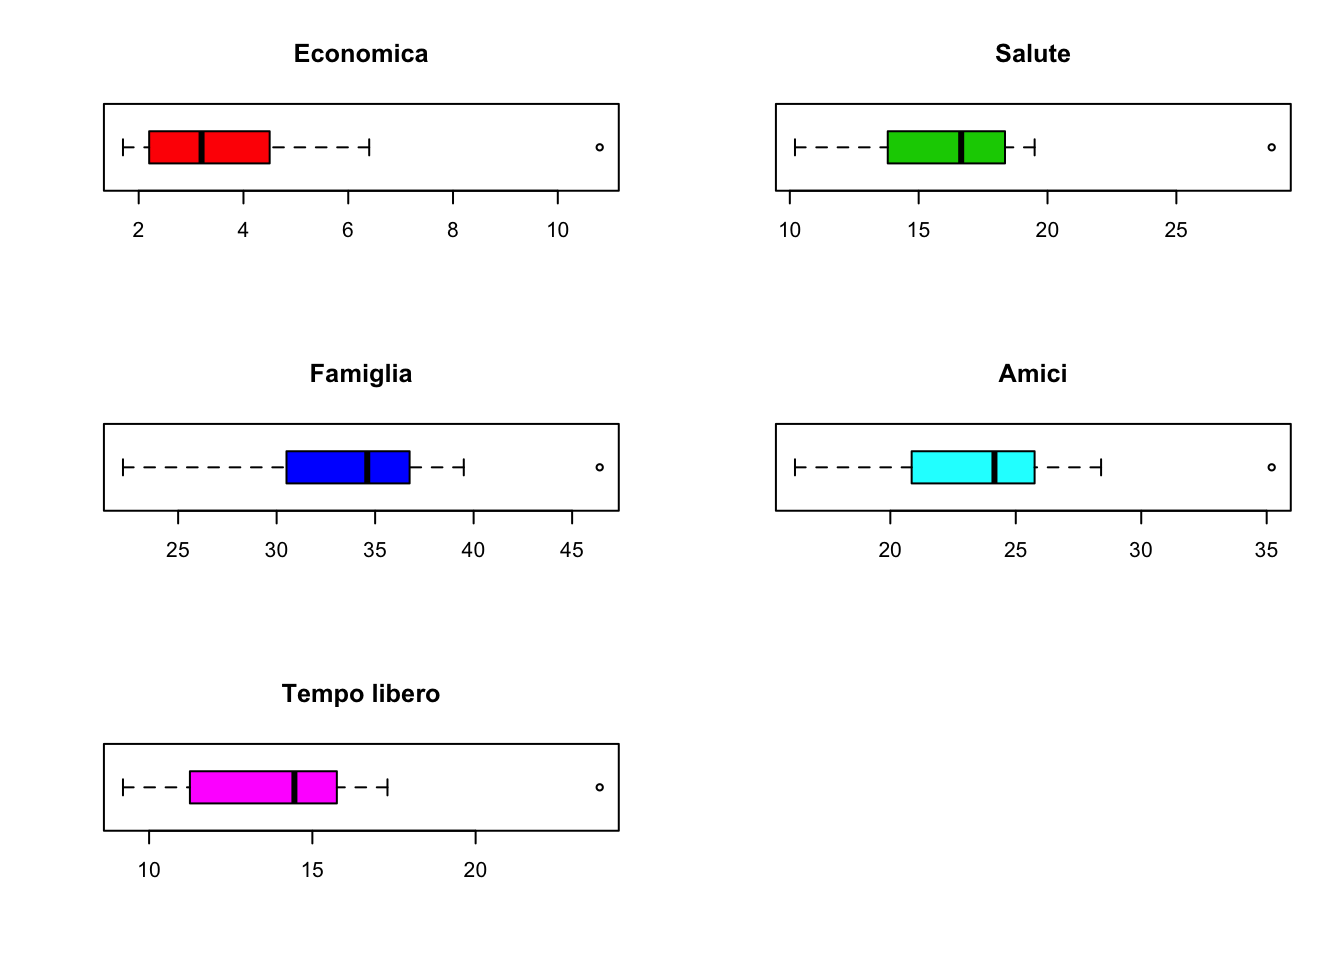
\includegraphics{statistics-project_files/figure-latex/boxplot-singoli-1} 

}

\caption{Boxplot}\label{fig:boxplot-singoli}
\end{figure}

Invece il seguente codice permette di mostrare tutti i boxplot nello
stesso grafico. Il grafico è mostrato nella figura
\ref{fig:boxplot-multiplo}.

\begin{Shaded}
\begin{Highlighting}[]
  \KeywordTok{boxplot}\NormalTok{(df, }\DataTypeTok{col =} \DecValTok{2}\OperatorTok{:}\DecValTok{6}\NormalTok{, }\DataTypeTok{names =}\NormalTok{ column.names)}
\end{Highlighting}
\end{Shaded}

\begin{figure}

{\centering 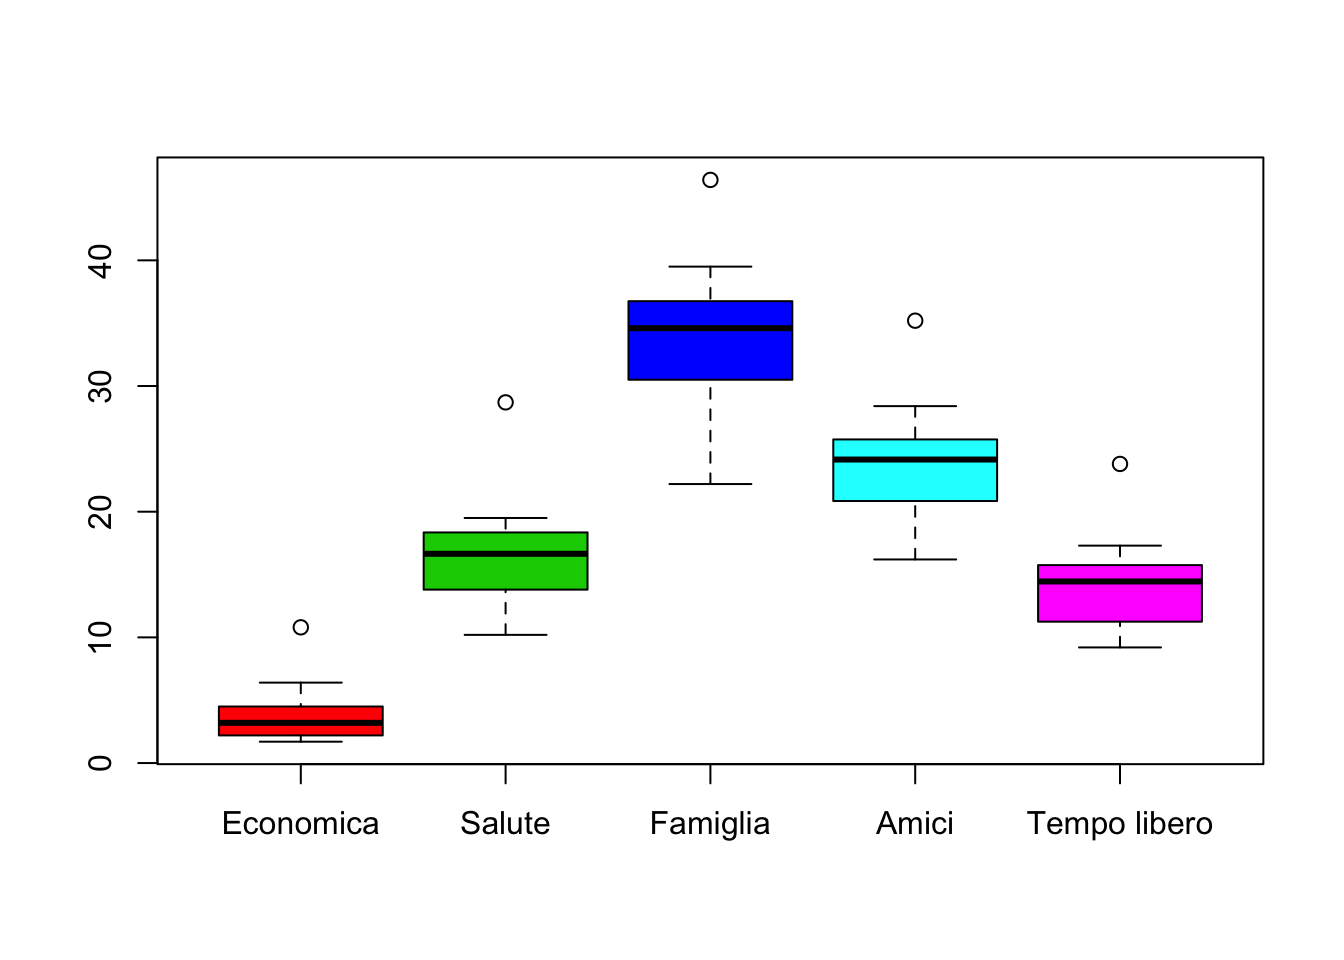
\includegraphics{statistics-project_files/figure-latex/boxplot-multiplo-1} 

}

\caption{Boxplot}\label{fig:boxplot-multiplo}
\end{figure}

Infine il seguente codice permette di calcolare i baffi i cui valori
sono mostrati nella tabella \ref{tab:baffi}.

\begin{Shaded}
\begin{Highlighting}[]
\NormalTok{calcolaBaffi <-}\StringTok{ }\ControlFlowTok{function}\NormalTok{(values) \{}
\NormalTok{  q <-}\StringTok{ }\KeywordTok{quantile}\NormalTok{(values)}
\NormalTok{  inferiore <-}\StringTok{ }\NormalTok{q[[}\DecValTok{2}\NormalTok{]] }\OperatorTok{-}\StringTok{ }\FloatTok{1.5} \OperatorTok{*}\StringTok{ }\NormalTok{(q[[}\DecValTok{4}\NormalTok{]] }\OperatorTok{-}\StringTok{ }\NormalTok{q[[}\DecValTok{2}\NormalTok{]])}
\NormalTok{  superiore <-}\StringTok{ }\NormalTok{q[[}\DecValTok{4}\NormalTok{]] }\OperatorTok{+}\StringTok{ }\FloatTok{1.5} \OperatorTok{*}\StringTok{ }\NormalTok{(q[[}\DecValTok{4}\NormalTok{]] }\OperatorTok{-}\StringTok{ }\NormalTok{q[[}\DecValTok{2}\NormalTok{]])}
\NormalTok{  baffoInf <-}\StringTok{ }\KeywordTok{min}\NormalTok{(values[values }\OperatorTok{>=}\StringTok{ }\NormalTok{inferiore])}
\NormalTok{  baffoSup <-}\StringTok{ }\KeywordTok{max}\NormalTok{(values[values }\OperatorTok{<=}\StringTok{ }\NormalTok{superiore])}
  \KeywordTok{c}\NormalTok{(baffoInf, baffoSup)  }
\NormalTok{\}}
\NormalTok{baffi <-}\StringTok{ }\KeywordTok{sapply}\NormalTok{(df, calcolaBaffi)}
\KeywordTok{row.names}\NormalTok{(baffi) <-}\StringTok{ }\KeywordTok{c}\NormalTok{(}\StringTok{"Inferiore"}\NormalTok{, }\StringTok{"Superiore"}\NormalTok{)}
\end{Highlighting}
\end{Shaded}

\begin{table}

\caption{\label{tab:baffi}Baffi}
\centering
\begin{tabular}[t]{l|r|r|r|r|r}
\hline
  & Economica & Salute & Famiglia & Amici & Tempo libero\\
\hline
Inferiore & 1.7 & 10.2 & 22.2 & 16.2 & 9.2\\
\hline
Superiore & 6.4 & 19.5 & 39.5 & 28.4 & 17.3\\
\hline
\end{tabular}
\end{table}

Dall'analisi visiva dei baffi si può trarre la conclusione che in ogni
caratteristica è presente un valore anomalo e per tutte le
caratteristiche l'individuo nel campione che presenta il valore anomale
è il ``Trentino Alto Adige''. Inoltre si può osservare che gli italiani
traggono in media il massimo della soddisfazione nei rapporti familiari
seguiti dai rapporti con gli amici, la salute, il tempo libero e infine
dalla situazione economica.

Si nota inoltre che la mediana è più vicina al terzo quartile e che il
baffo sinistro è più grande del destro per tutte le caratteristiche
eccetto per la soddisfazione economica.

\chapter{Distribuzione}\label{distribuzione}

In questo capitolo verranno prima calcolate e analizzate le frequenze
delle caratteristiche del data set, in seguito le frequenze saranno
utilizzate per il calcolo della distribuzione empirica continua di
frequenza per ogni caratteristica. Il capitolo si concluderà con un
analisi della simmetria e della curtosi delle distribuzioni considerate.

\section{Frequenze}\label{frequenze}

Se i valori osservati possono assumere \(k\) modalità, la frequenza
assoluta della modalità \(i\)-esima è definita come il numero di
occorrenze della modalità \(i\)-esima nel campione. Mentre la frequenza
relativa della modalità \(i\)-esima è definita come il rapporto tra la
frequenza assoluta \(i\)-esima ed il numero delle osservazioni. Infine
la frequenza cumulata assoluta (o relativa) \(i\)-esima è definita come
la somma di tutte le frequenze assolute (o relative) \(j\)-esime con
\(j\) minore o uguale a \(i\).

Il calcolo delle frequenze diventa problematico nel caso in cui il
numero delle modalità è grande (o al limite infinito), rispetto al
numero delle osservazioni. Infatti le frequenze tenderanno ad assumere
valori pari a zero o uno. In questi casi è utile dividere i valori in
classi e considerare tali classi come le modalità osservabili.

Essendo il nostro data set composto da dati reali si è scelto, per il
motivo sopra esposto, di dividere i dati in classi in modo tale che ogni
numero reale appartenga alla classe del suo intero più vicino.

Il seguente codice permette di calcolare le frequenze relative del
dataset. I valori calcolati sono mostrati nelle tabelle
\ref{tab:frequenze-1}, \ref{tab:frequenze-2}, \ref{tab:frequenze-3}
\ref{tab:frequenze-4} e \ref{tab:frequenze-5}, per le classi non
presenti nelle tabelle la frequenza relativa associata è nulla. Invece
una rappresentazione delle frequenze con grafici a bastoncini è mostrata
nelle figure \ref{fig:bastoncini-frequenze-1},
\ref{fig:bastoncini-frequenze-2}, \ref{fig:bastoncini-frequenze-3},
\ref{fig:bastoncini-frequenze-4} e \ref{fig:bastoncini-frequenze-5}
rispettivamente per le stesse caratteristiche. Nei grafici la linea
rossa indica la mediana mentre la linea verde la media.

\begin{Shaded}
\begin{Highlighting}[]
\NormalTok{classi <-}\StringTok{ }\KeywordTok{c}\NormalTok{(}\DecValTok{0}\NormalTok{, }\KeywordTok{seq}\NormalTok{(}\FloatTok{0.5}\NormalTok{, }\FloatTok{100.5}\NormalTok{, }\DataTypeTok{by =} \DecValTok{1}\NormalTok{))}

\NormalTok{calcolaFrequenzeRelative =}\StringTok{ }\ControlFlowTok{function}\NormalTok{(x) \{}
  \KeywordTok{table}\NormalTok{(}\KeywordTok{cut}\NormalTok{(x, }\DataTypeTok{breaks =}\NormalTok{ classi, }\DataTypeTok{right =} \OtherTok{FALSE}\NormalTok{)) }\OperatorTok{/}\StringTok{ }\NormalTok{rowCount  }
\NormalTok{\}}

\NormalTok{frequenzeRelative <-}\StringTok{ }\KeywordTok{sapply}\NormalTok{(df, calcolaFrequenzeRelative)}
\end{Highlighting}
\end{Shaded}

\begin{table}

\caption{\label{tab:frequenze-1}Frequenze relative - Soddisfazione Economica}
\centering
\begin{tabular}[t]{l|l}
\hline
Classe & Frequenza Relativa\\
\hline
[1.5,2.5) & 0.3\\
\hline
[2.5,3.5) & 0.25\\
\hline
[3.5,4.5) & 0.2\\
\hline
[4.5,5.5) & 0.15\\
\hline
[5.5,6.5) & 0.05\\
\hline
[10.5,11.5) & 0.05\\
\hline
\end{tabular}
\end{table}\begin{table}

\caption{\label{tab:frequenze-2}Frequenze relative - Soddisfazione Salute}
\centering
\begin{tabular}[t]{l|l}
\hline
Classe & Frequenza Relativa\\
\hline
[9.5,10.5) & 0.05\\
\hline
[10.5,11.5) & 0.05\\
\hline
[11.5,12.5) & 0.1\\
\hline
[12.5,13.5) & 0.05\\
\hline
[14.5,15.5) & 0.15\\
\hline
[15.5,16.5) & 0.1\\
\hline
[16.5,17.5) & 0.1\\
\hline
[17.5,18.5) & 0.2\\
\hline
[18.5,19.5) & 0.1\\
\hline
[19.5,20.5) & 0.05\\
\hline
[28.5,29.5) & 0.05\\
\hline
\end{tabular}
\end{table}\begin{table}

\caption{\label{tab:frequenze-3}Frequenze relative - Soddisfazione Famiglia}
\centering
\begin{tabular}[t]{l|l}
\hline
Classe & Frequenza Relativa\\
\hline
[21.5,22.5) & 0.05\\
\hline
[23.5,24.5) & 0.05\\
\hline
[27.5,28.5) & 0.05\\
\hline
[29.5,30.5) & 0.05\\
\hline
[30.5,31.5) & 0.2\\
\hline
[33.5,34.5) & 0.1\\
\hline
[34.5,35.5) & 0.1\\
\hline
[35.5,36.5) & 0.15\\
\hline
[36.5,37.5) & 0.05\\
\hline
[38.5,39.5) & 0.1\\
\hline
[39.5,40.5) & 0.05\\
\hline
[45.5,46.5) & 0.05\\
\hline
\end{tabular}
\end{table}\begin{table}

\caption{\label{tab:frequenze-4}Frequenze relative - Soddisfazione Amici}
\centering
\begin{tabular}[t]{l|l}
\hline
Classe & Frequenza Relativa\\
\hline
[15.5,16.5) & 0.05\\
\hline
[16.5,17.5) & 0.05\\
\hline
[17.5,18.5) & 0.05\\
\hline
[19.5,20.5) & 0.1\\
\hline
[21.5,22.5) & 0.1\\
\hline
[22.5,23.5) & 0.1\\
\hline
[23.5,24.5) & 0.05\\
\hline
[24.5,25.5) & 0.15\\
\hline
[25.5,26.5) & 0.15\\
\hline
[26.5,27.5) & 0.1\\
\hline
[27.5,28.5) & 0.05\\
\hline
[34.5,35.5) & 0.05\\
\hline
\end{tabular}
\end{table}\begin{table}

\caption{\label{tab:frequenze-5}Frequenze relative - Soddisfazione Tempo libero}
\centering
\begin{tabular}[t]{l|l}
\hline
Classe & Frequenza Relativa\\
\hline
[8.5,9.5) & 0.15\\
\hline
[10.5,11.5) & 0.1\\
\hline
[11.5,12.5) & 0.15\\
\hline
[12.5,13.5) & 0.05\\
\hline
[13.5,14.5) & 0.05\\
\hline
[14.5,15.5) & 0.15\\
\hline
[15.5,16.5) & 0.2\\
\hline
[16.5,17.5) & 0.1\\
\hline
[23.5,24.5) & 0.05\\
\hline
\end{tabular}
\end{table}

\begin{figure}

{\centering 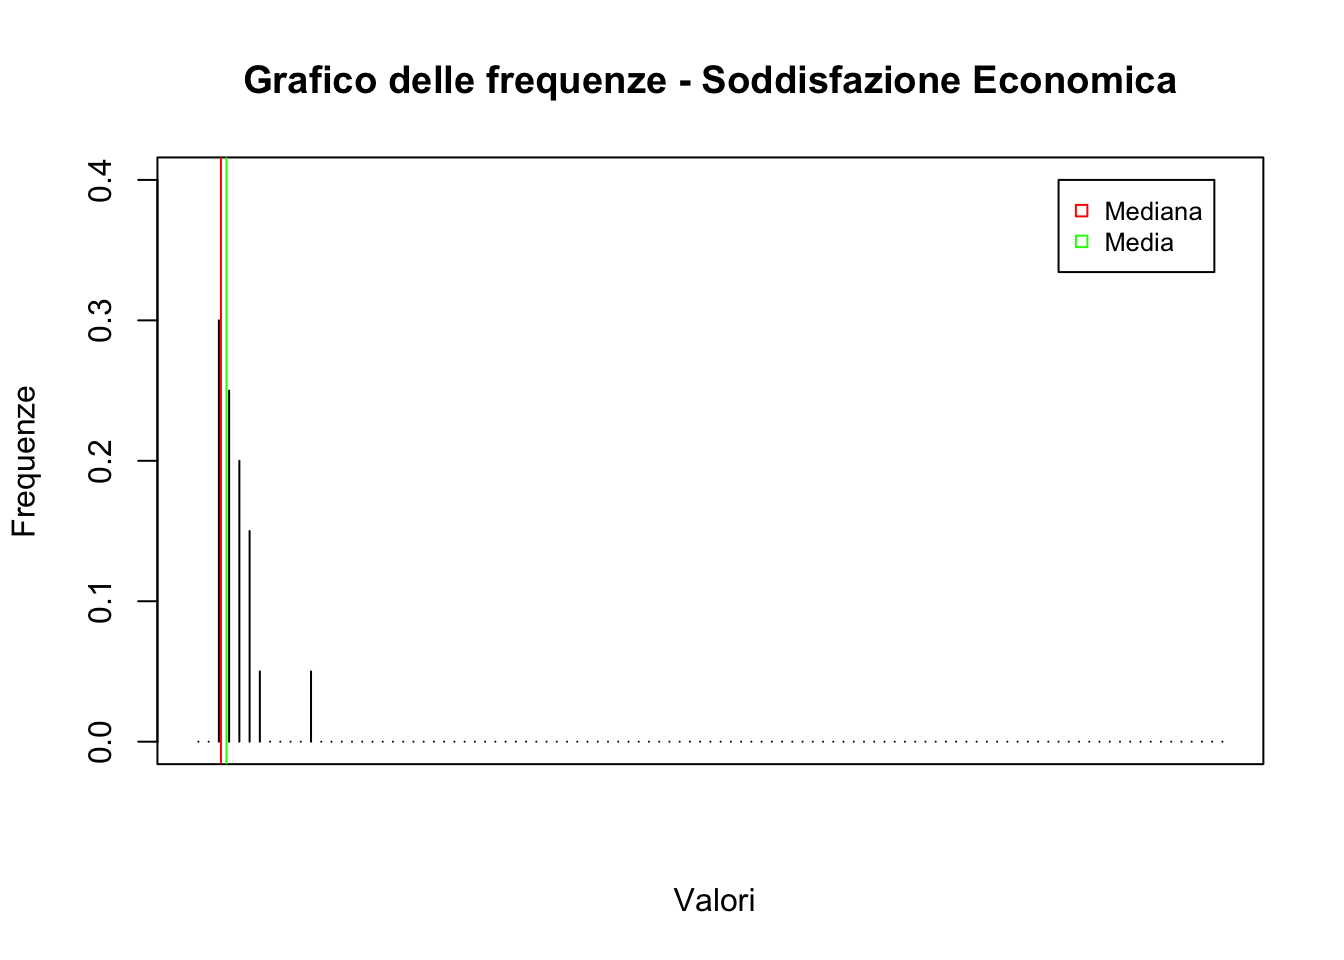
\includegraphics{statistics-project_files/figure-latex/bastoncini-frequenze-1-1} 

}

\caption{Grafico delle frequenze - Soddisfazione Economica}\label{fig:bastoncini-frequenze-1}
\end{figure}\begin{figure}

{\centering 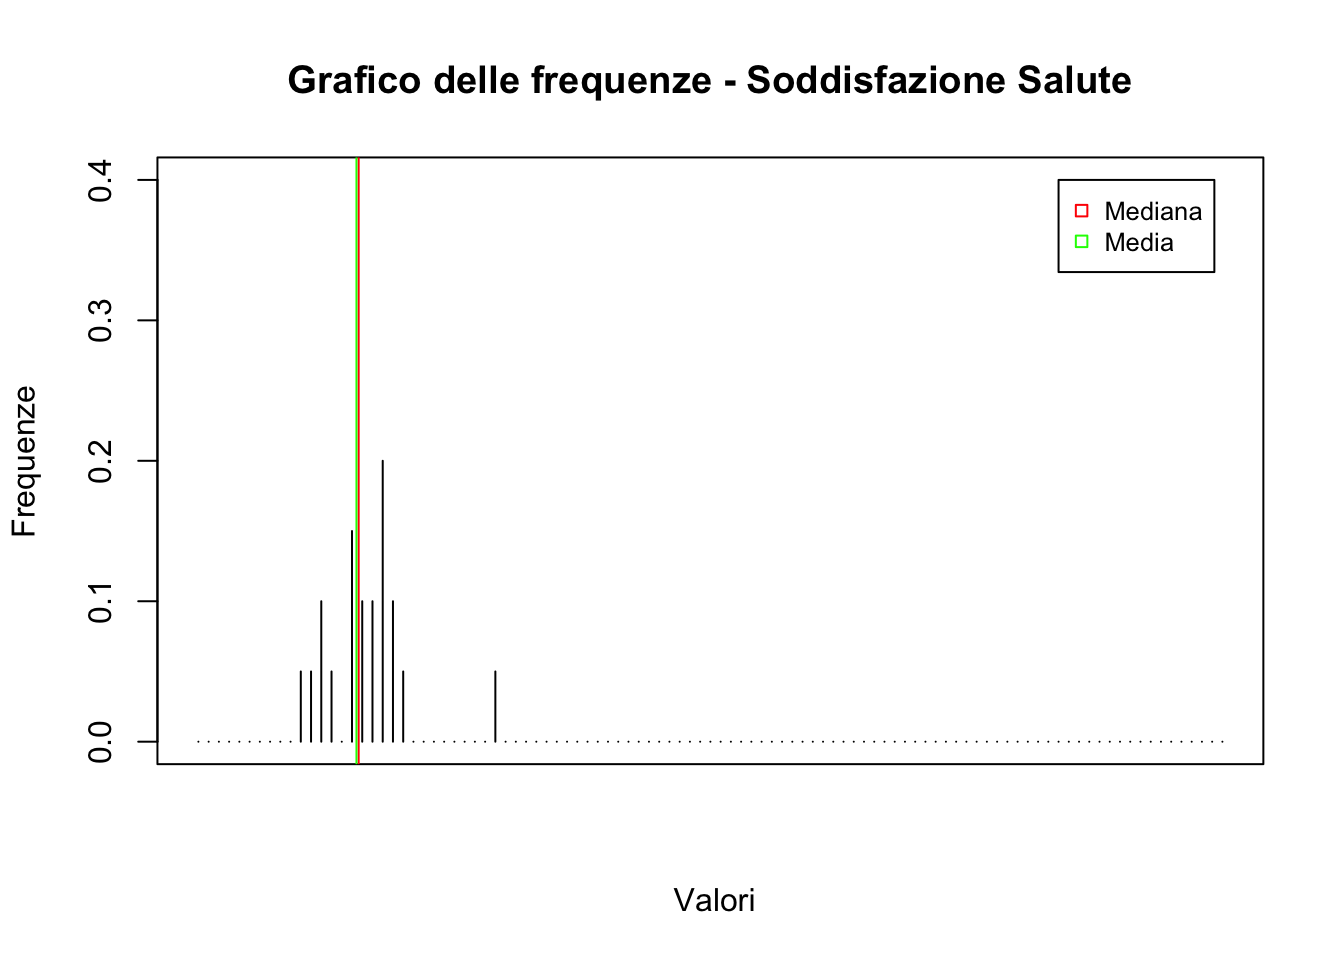
\includegraphics{statistics-project_files/figure-latex/bastoncini-frequenze-2-1} 

}

\caption{Grafico delle frequenze - Soddisfazione Salute}\label{fig:bastoncini-frequenze-2}
\end{figure}

\begin{figure}

{\centering 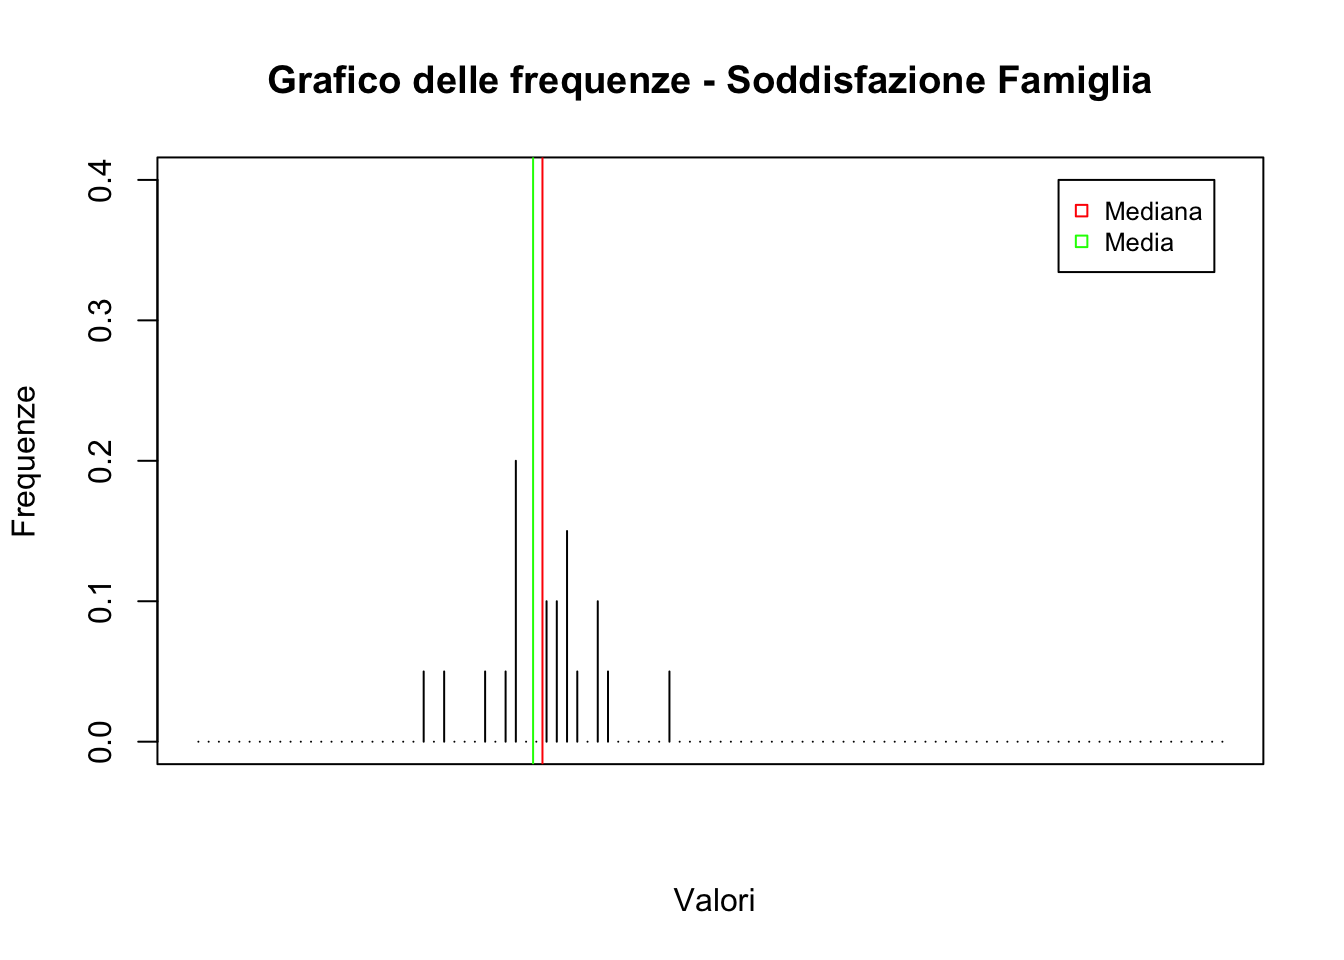
\includegraphics{statistics-project_files/figure-latex/bastoncini-frequenze-3-1} 

}

\caption{Grafico delle frequenze - Soddisfazione Famiglia}\label{fig:bastoncini-frequenze-3}
\end{figure}

\begin{figure}

{\centering 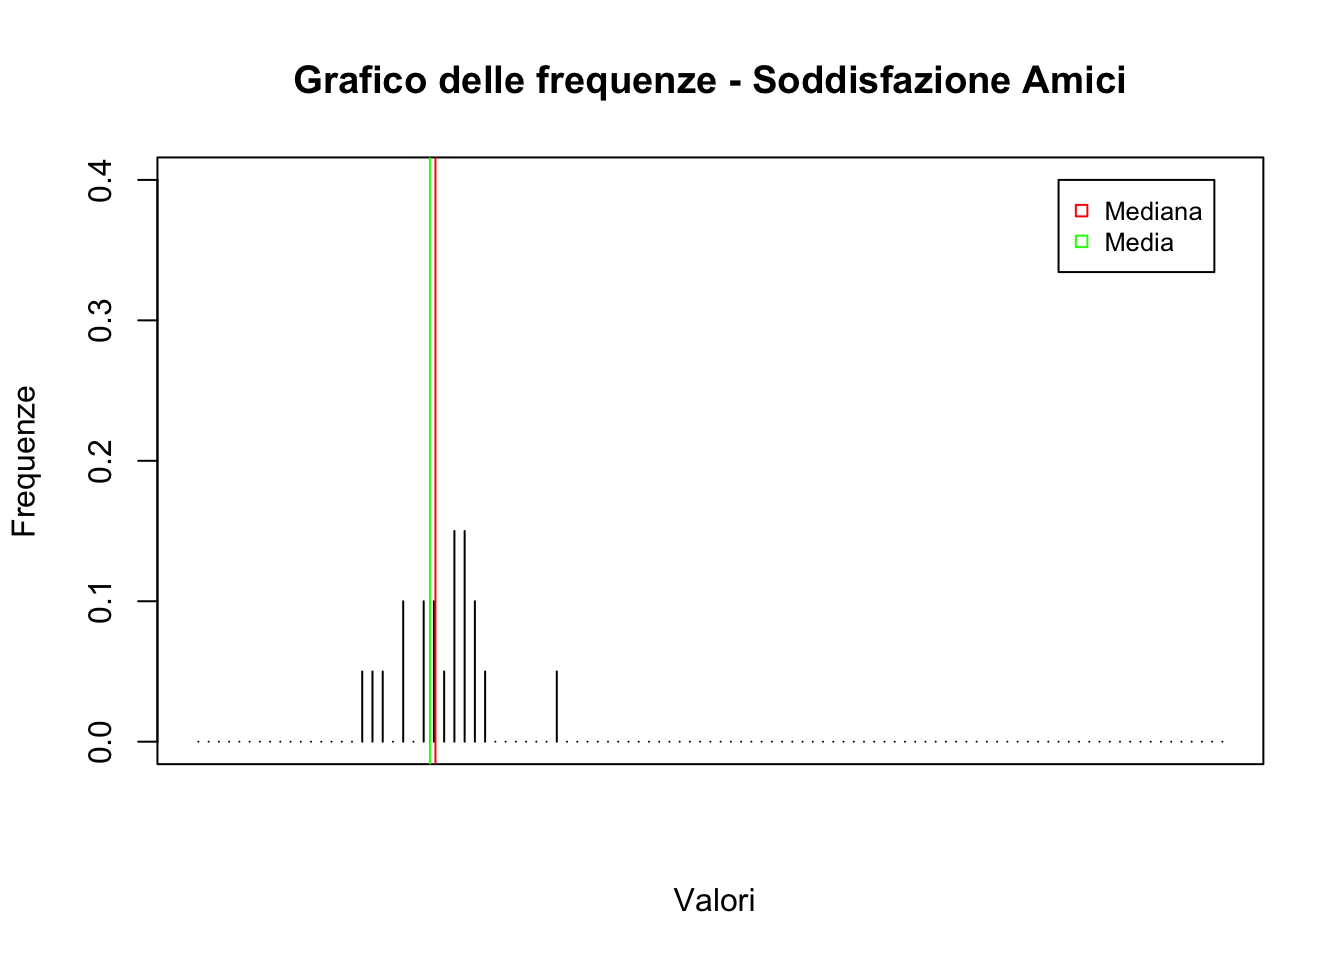
\includegraphics{statistics-project_files/figure-latex/bastoncini-frequenze-4-1} 

}

\caption{Grafico delle frequenze - Soddisfazione Amici}\label{fig:bastoncini-frequenze-4}
\end{figure}

\begin{figure}

{\centering 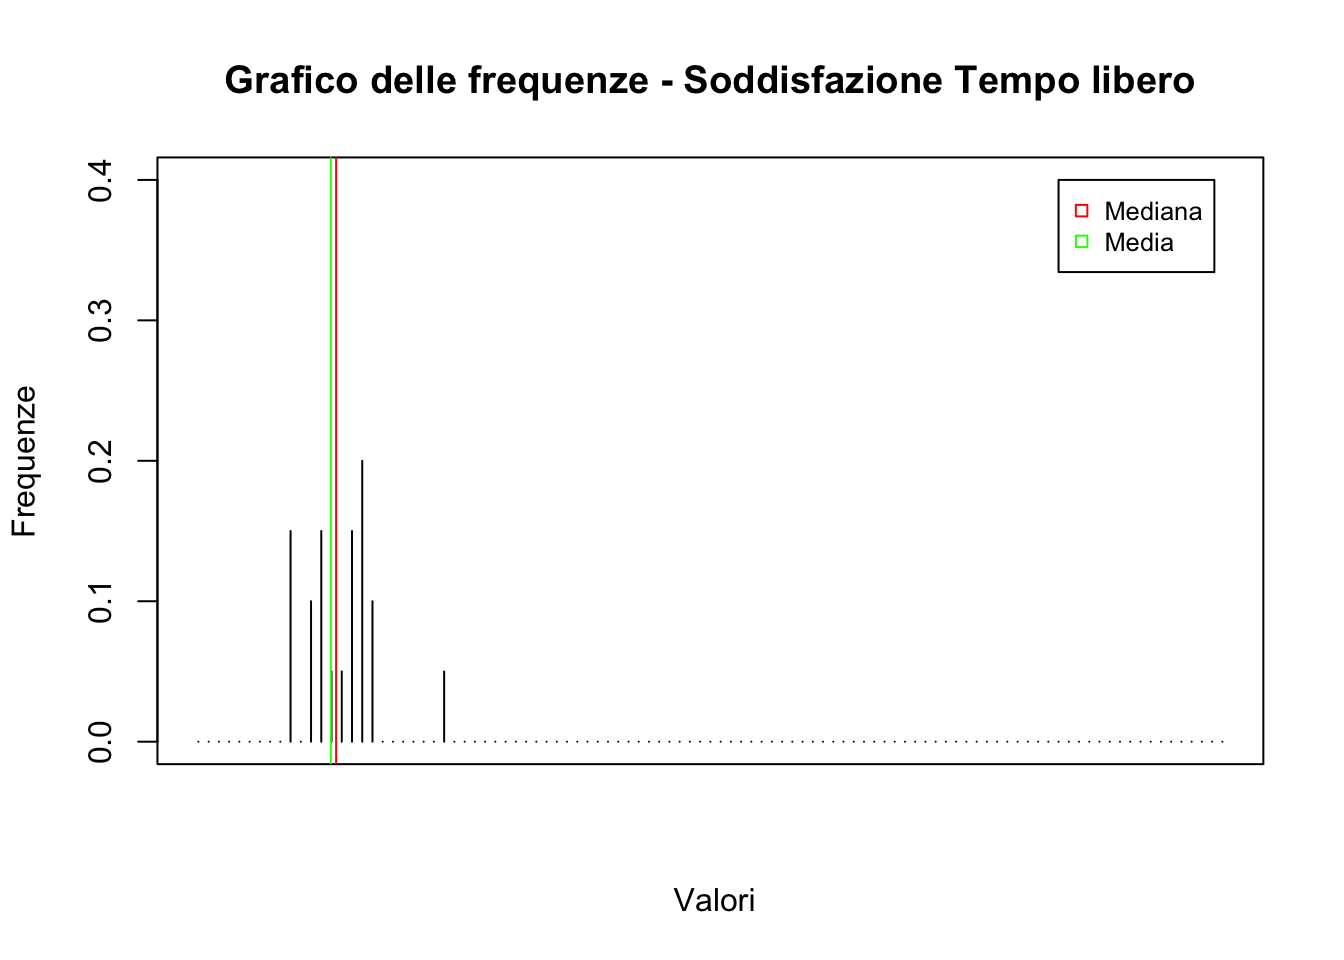
\includegraphics{statistics-project_files/figure-latex/bastoncini-frequenze-5-1} 

}

\caption{Grafico delle frequenze - Soddisfazione Tempo libero}\label{fig:bastoncini-frequenze-5}
\end{figure}

\section{Funzione di distribuzione empirica
continua}\label{funzione-di-distribuzione-empirica-continua}

La funzione di distribuzione empirica continua è una funzione che
associa a ogni valore reale \(x\) la frequenza che un valore osservato
sia minore o uguale a \(x\). Da notare che nel continuo si preferisce
suddividere i valori in \(k\) classi \([z_i, z_{i+1})\) con
\(i = 1,..,k\). Ne consegue che la distribuzione empirica continua è una
funzione reale non decrescente, che assume valore zero per ogni reale
minore di \(z_1\) e valore uno per ogni reale maggiore o uguale a
\(z_{k+1}\), quando \(x = z_i\) per \(i = 1,..,k\) la funzione assume lo
stesso valore della frequenza relativa cumulata \(F_i\) mentre per ogni
valore compreso tra \((z_i, z_{i+1})\) la funzione coincide con il
segmento passante per i punti \((z_i, F_i)\) e \((z_{i+1}, F_{i+1})\)

La seguente funzione permette di creare i grafici delle distribuzioni
empiriche continue delle caratteristiche del dataset, tali grafici sono
mostrati nelle figure \ref{fig:distribuzione-empirica1},
\ref{fig:distribuzione-empirica2}, \ref{fig:distribuzione-empirica3},
\ref{fig:distribuzione-empirica4}, \ref{fig:distribuzione-empirica5}.

\begin{Shaded}
\begin{Highlighting}[]
\NormalTok{distribuzioneEmpiricaContinua =}\StringTok{ }\ControlFlowTok{function}\NormalTok{(index, lim) \{}
\NormalTok{  x <-frequenzeRelative[, index]}
\NormalTok{  Fi<-}\KeywordTok{cumsum}\NormalTok{(x)}
\NormalTok{  Fi<-}\KeywordTok{c}\NormalTok{(}\DecValTok{0}\NormalTok{,Fi)}
\NormalTok{  main =}\StringTok{ }\KeywordTok{paste}\NormalTok{(}\StringTok{"Distribuzione empirica continua - Soddisfazione"}\NormalTok{, column.names[index])}
  \KeywordTok{plot}\NormalTok{(classi, Fi, }\DataTypeTok{type =} \StringTok{"l"}\NormalTok{,}\DataTypeTok{axes =} \OtherTok{FALSE}\NormalTok{, }
       \DataTypeTok{main =}\NormalTok{ main,}\DataTypeTok{col=}\StringTok{"red"}\NormalTok{, }
       \DataTypeTok{xlab =} \StringTok{" "}\NormalTok{, }\DataTypeTok{ylab =} \StringTok{" "}\NormalTok{,}
       \DataTypeTok{xlim =} \KeywordTok{c}\NormalTok{(}\DecValTok{0}\NormalTok{, lim))}
  \KeywordTok{axis}\NormalTok{(}\DecValTok{1}\NormalTok{, classi)}
  \KeywordTok{axis}\NormalTok{(}\DecValTok{2}\NormalTok{, }\KeywordTok{format}\NormalTok{(Fi, }\DataTypeTok{digits =} \DecValTok{1}\NormalTok{), }\DataTypeTok{las =} \DecValTok{2}\NormalTok{)}
  \KeywordTok{box}\NormalTok{()}
\NormalTok{\}}
\end{Highlighting}
\end{Shaded}

\begin{figure}

{\centering 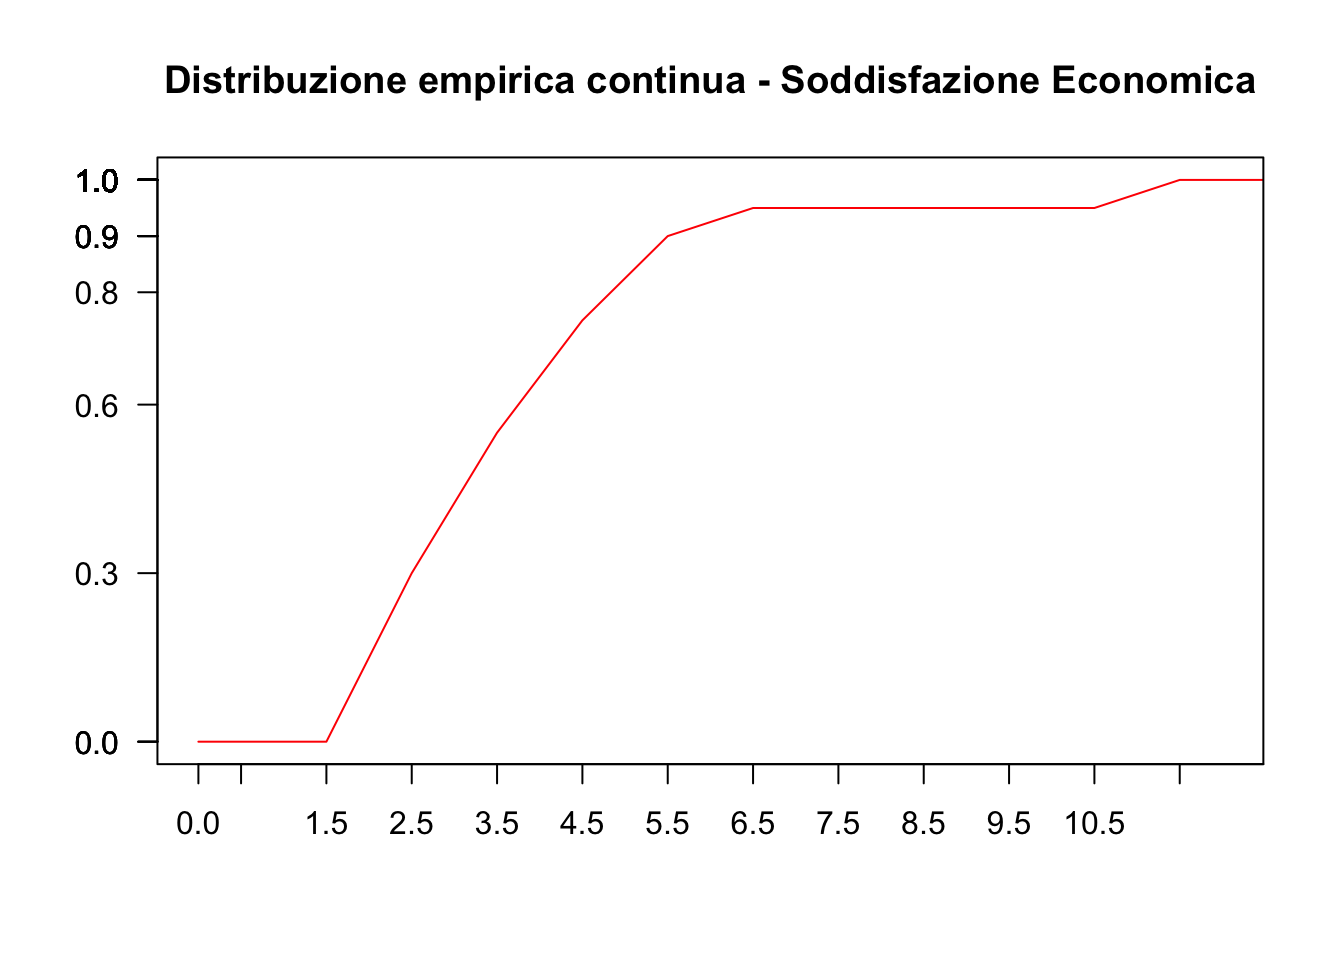
\includegraphics{statistics-project_files/figure-latex/distribuzione-empirica1-1} 

}

\caption{Distribuzione empirica continua - Soddisfazione Economica}\label{fig:distribuzione-empirica1}
\end{figure}

\begin{figure}

{\centering 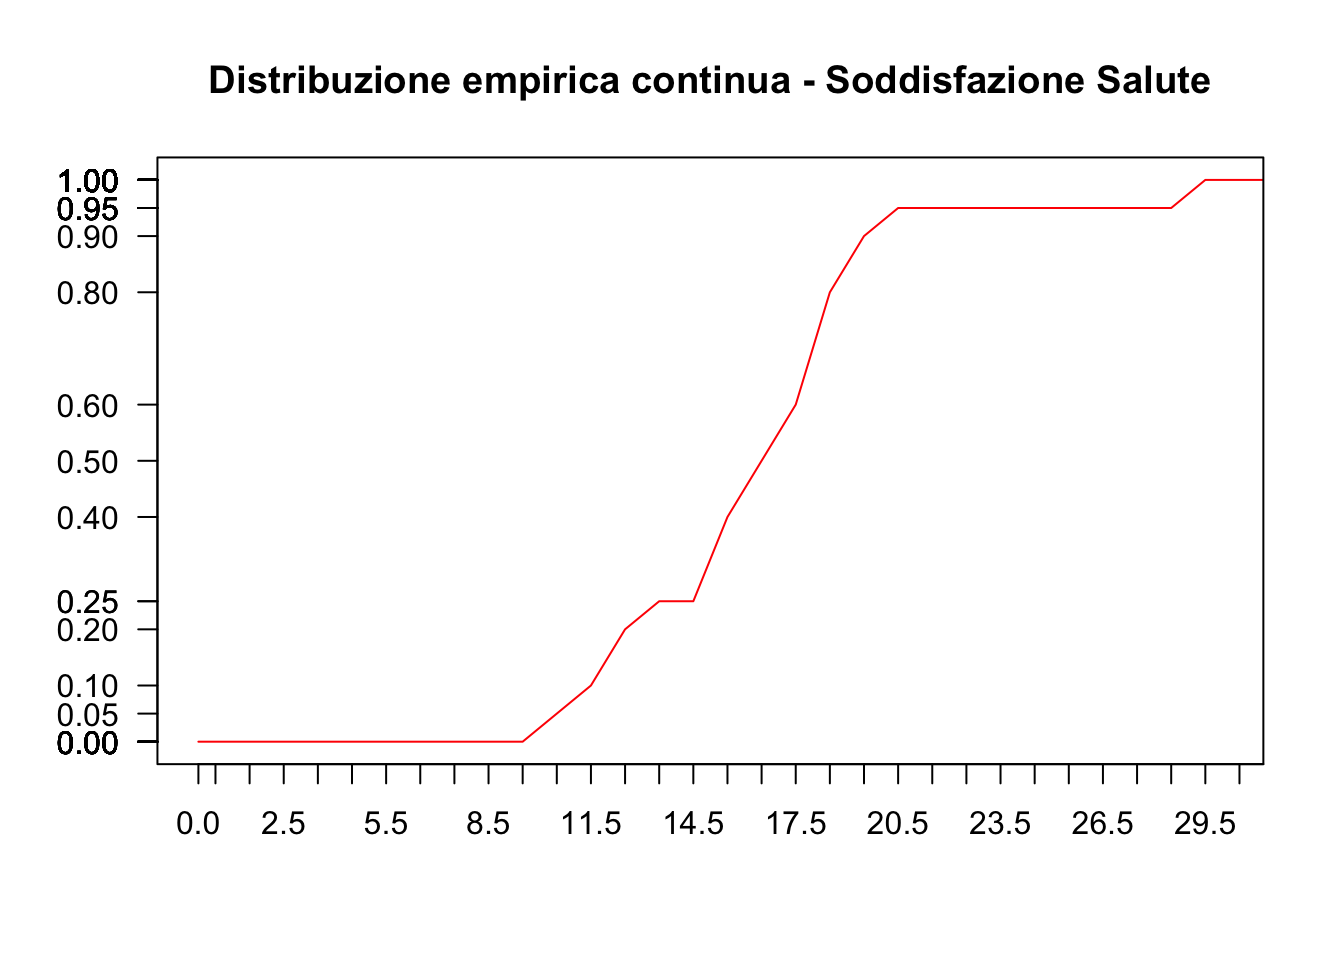
\includegraphics{statistics-project_files/figure-latex/distribuzione-empirica2-1} 

}

\caption{Distribuzione empirica continua - Soddisfazione Salute}\label{fig:distribuzione-empirica2}
\end{figure}

\begin{figure}

{\centering 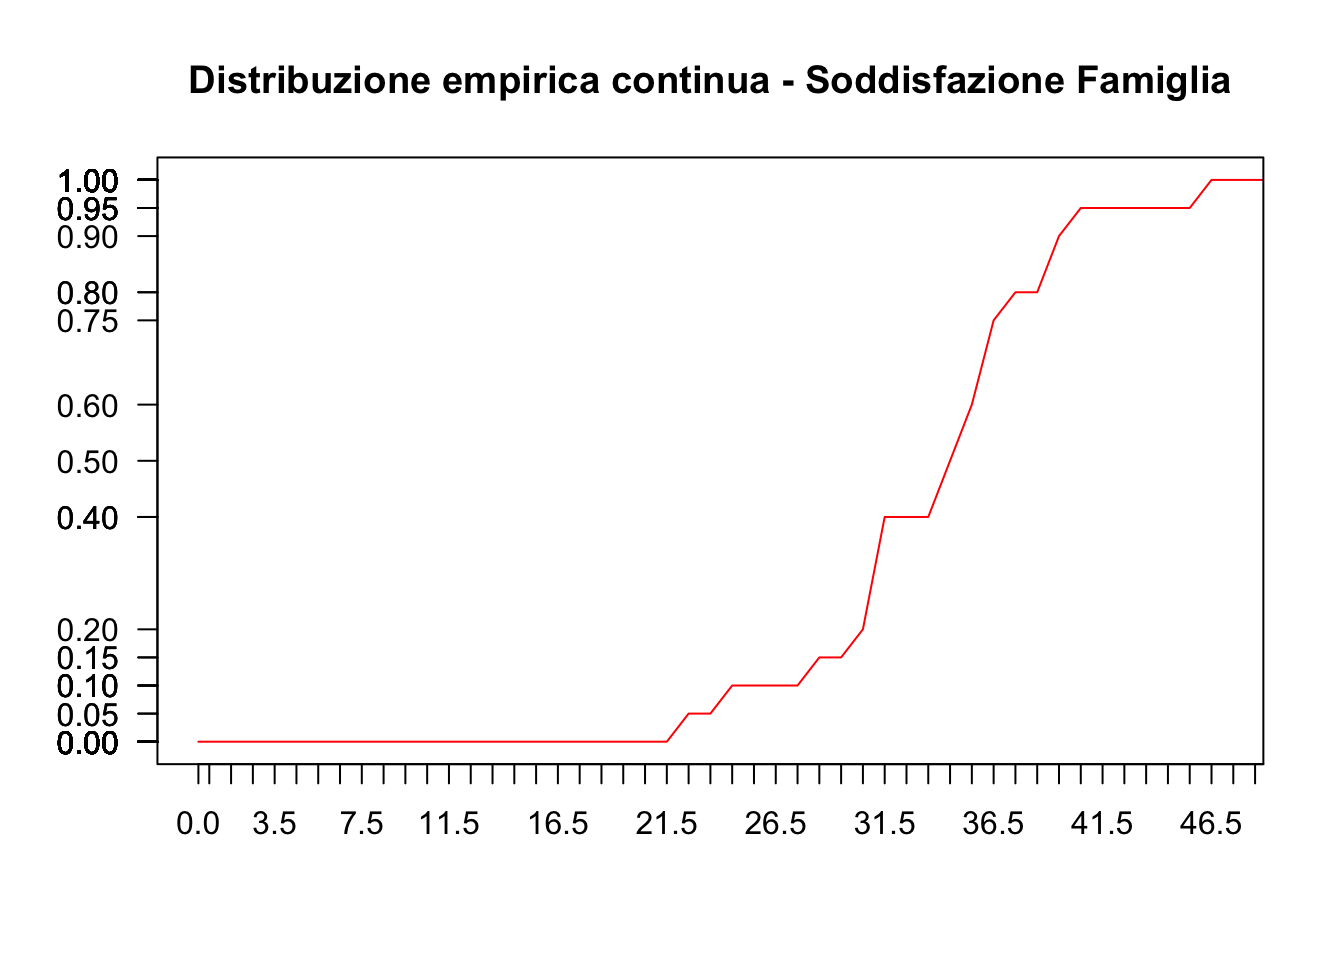
\includegraphics{statistics-project_files/figure-latex/distribuzione-empirica3-1} 

}

\caption{Distribuzione empirica continua - Soddisfazione Famiglia}\label{fig:distribuzione-empirica3}
\end{figure}

\begin{figure}

{\centering 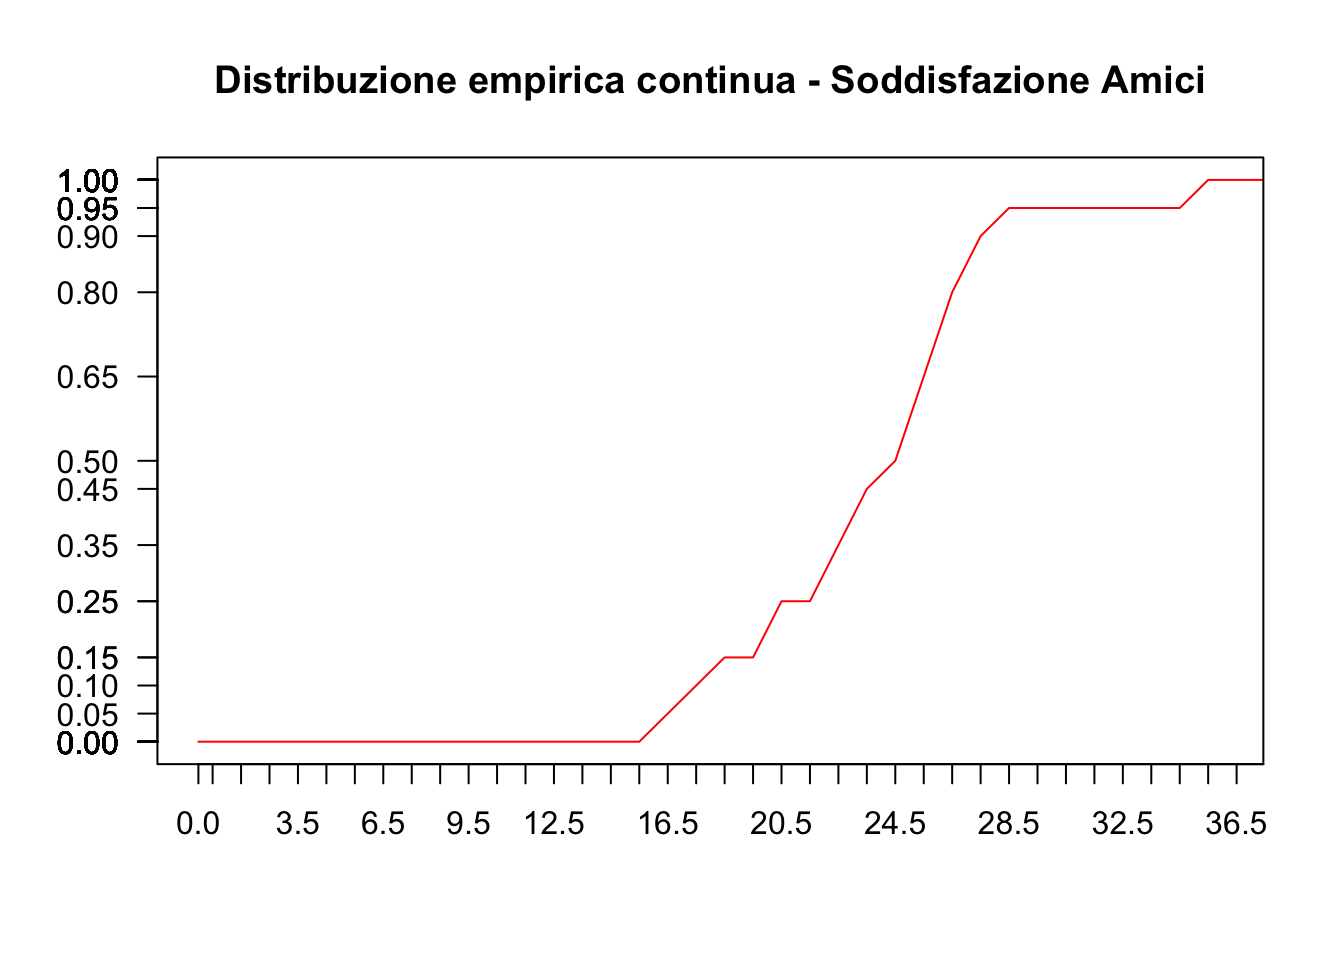
\includegraphics{statistics-project_files/figure-latex/distribuzione-empirica4-1} 

}

\caption{Distribuzione empirica continua - Soddisfazione Amici}\label{fig:distribuzione-empirica4}
\end{figure}

\begin{figure}

{\centering 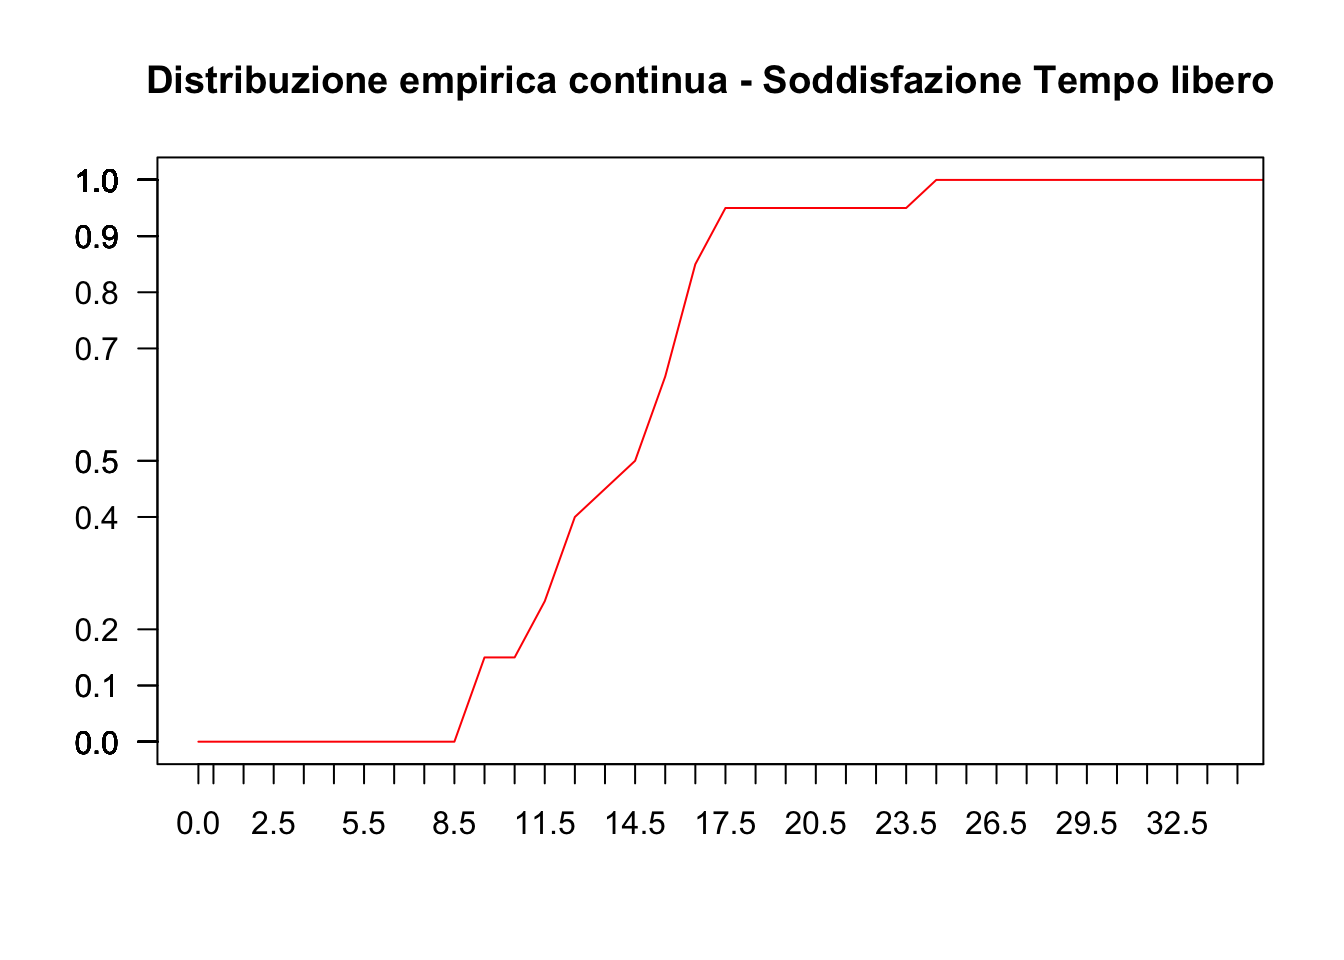
\includegraphics{statistics-project_files/figure-latex/distribuzione-empirica5-1} 

}

\caption{Distribuzione empirica continua - Soddisfazione Tempo Libero}\label{fig:distribuzione-empirica5}
\end{figure}

\section{Istogrammi}\label{istogrammi}

Gli istogrammi sono una rappresentazione grafica della distribuzione
delle frequenze in classi. Graficamente sono costituiti da rettangoli i
cui estremi delle basi coincidono con gli estremi delle classi. Inoltre
le aree dei rettangoli sono uguali alla frequenza assoluta o relativa
delle rispettive classi.

Il seguente codice permette di disegnare gli istogrammi per le
caratteristiche del data set. I grafici sono mostrati in figura
\ref{fig:istrogrammi}.

\begin{Shaded}
\begin{Highlighting}[]
\KeywordTok{par}\NormalTok{(}\DataTypeTok{mfrow=}\KeywordTok{c}\NormalTok{(}\DecValTok{3}\NormalTok{, }\DecValTok{2}\NormalTok{))}
\ControlFlowTok{for}\NormalTok{ (i }\ControlFlowTok{in} \DecValTok{1}\OperatorTok{:}\NormalTok{colCount) \{}
  \KeywordTok{hist}\NormalTok{(df[[i]], }\DataTypeTok{freq =} \OtherTok{TRUE}\NormalTok{,}
     \DataTypeTok{main =} \KeywordTok{paste}\NormalTok{(}\StringTok{"Istogramma - "}\NormalTok{, column.names[i]), }
     \DataTypeTok{ylab =} \StringTok{"Frequenza assoluta"}\NormalTok{, }
     \DataTypeTok{xlab =} \KeywordTok{paste}\NormalTok{(}\StringTok{"Soddifazione - "}\NormalTok{, column.names[i]))}
\NormalTok{\}}
\end{Highlighting}
\end{Shaded}

\begin{figure}

{\centering 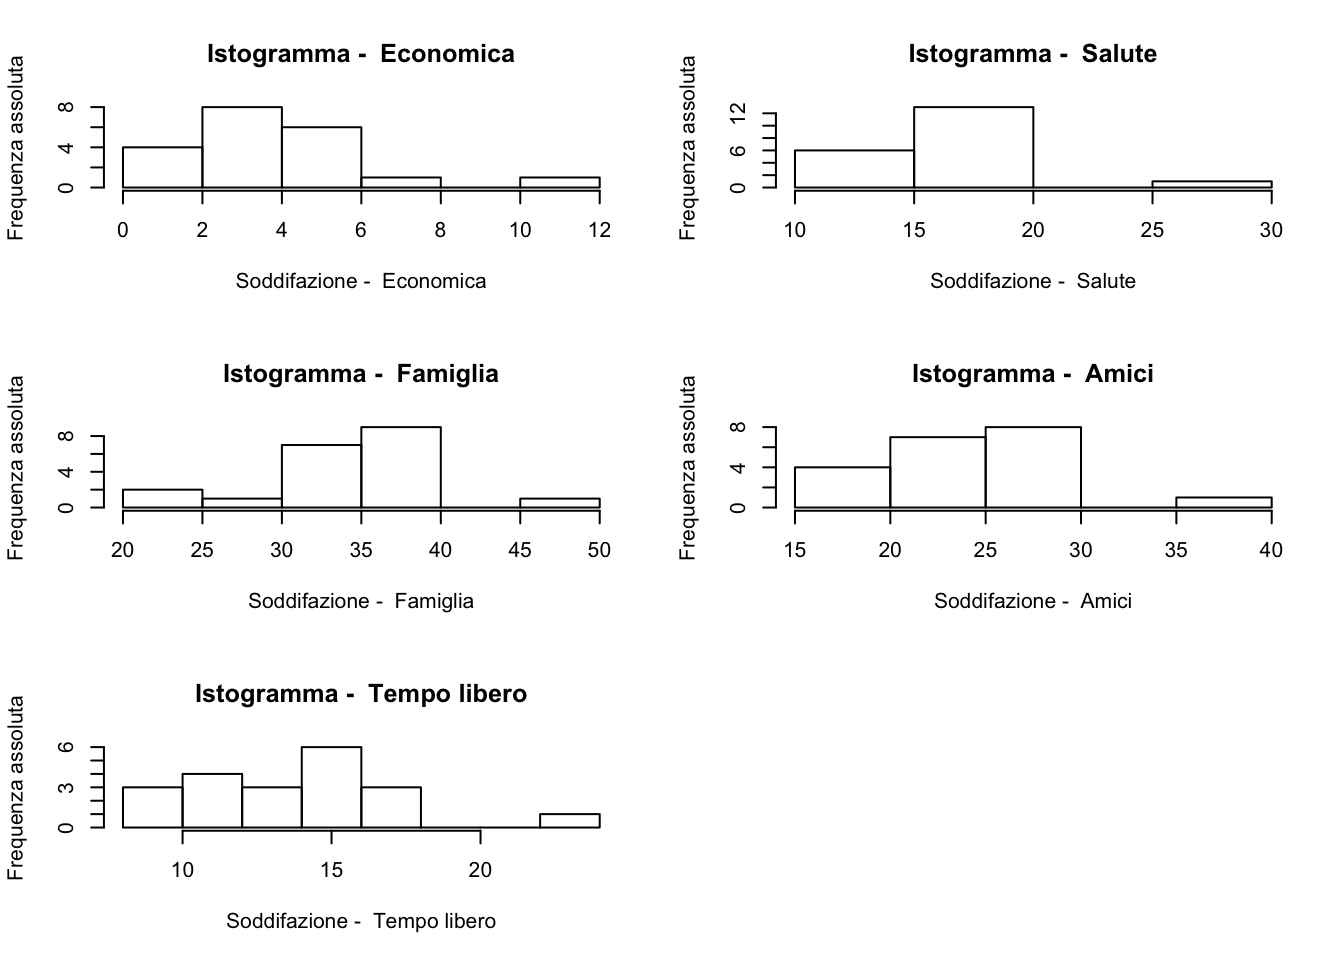
\includegraphics{statistics-project_files/figure-latex/istrogrammi-1} 

}

\caption{Istrogrammi}\label{fig:istrogrammi}
\end{figure}

\section{Simmetria}\label{simmetria}

In questo paragrafo analizzeremo la simmetria della distribuzione di
frequenza tramite un indice detto Skewness campionario definito con il
valore \[\gamma_1=\frac{m_3}{m_2^{3/2}} \] dove
\[m_j = \frac{1}{n}\sum_{i=1}^{n}(x_i-\overline{x})^j\] è detto momento
centrato campionario j-esimo.

La skewness campionaria assume il valore zero se la distribuzione è
simmetrica, valori positivi nel caso di asimmetria positiva (sbilanciata
a destra) o valori negativi nel caso di asimmetria negativa (sbilanciata
a sinistra). Da notare che è Skewness campionaria è un numero puro.

Va inoltre notato che esistono distribuzioni non simmetriche con
skewness campionaria pari a zero. Ne consegue che il valore zero è una
condizione necessaria ma non sufficiente affinché la distribuzione sia
simmetrica.

Il seguente codice permette di calcolare la Skewness campionaria e il
tipo di simmetria. I valori ottenuti sono mostrati rispettivamente nelle
tabelle \ref{tab:skewness} e \ref{tab:tipoSimmetria}

\begin{Shaded}
\begin{Highlighting}[]
\NormalTok{mcc <-}\ControlFlowTok{function}\NormalTok{(x, j)\{}
      \KeywordTok{sum}\NormalTok{((x }\OperatorTok{-}\StringTok{ }\KeywordTok{mean}\NormalTok{(x))}\OperatorTok{^}\NormalTok{j) }\OperatorTok{/}\StringTok{ }\KeywordTok{length}\NormalTok{(x)}
\NormalTok{\}}

\NormalTok{skw <-}\ControlFlowTok{function}\NormalTok{(x) \{}
    \KeywordTok{mcc}\NormalTok{(x, }\DecValTok{3}\NormalTok{) }\OperatorTok{/}\StringTok{ }\KeywordTok{mcc}\NormalTok{(x, }\DecValTok{2}\NormalTok{) }\OperatorTok{^}\StringTok{ }\FloatTok{1.5}
\NormalTok{\}}

\NormalTok{tipoSimmetria <-}\StringTok{ }\ControlFlowTok{function}\NormalTok{(x) \{}
  \ControlFlowTok{if}\NormalTok{ (x }\OperatorTok{==}\StringTok{ }\DecValTok{0}\NormalTok{) \{}
    \StringTok{"simmetrica"}
\NormalTok{  \} }\ControlFlowTok{else} \ControlFlowTok{if}\NormalTok{ (x }\OperatorTok{>}\StringTok{ }\DecValTok{0}\NormalTok{) \{}
    \StringTok{"asimmetria positiva"}
\NormalTok{  \} }\ControlFlowTok{else}\NormalTok{ \{}
    \StringTok{"asimmetria negativa"}
\NormalTok{  \}}
\NormalTok{\}}

\NormalTok{skewness <-}\StringTok{ }\KeywordTok{sapply}\NormalTok{(df, skw)}

\NormalTok{tipoSimmetria <-}\StringTok{ }\KeywordTok{as.matrix}\NormalTok{(}\KeywordTok{sapply}\NormalTok{(skewness, tipoSimmetria))}
\KeywordTok{colnames}\NormalTok{(tipoSimmetria) <-}\StringTok{ "Simmetria"}
\end{Highlighting}
\end{Shaded}

\begin{table}

\caption{\label{tab:skewness}Skewness campionaria}
\centering
\begin{tabular}[t]{l|l}
\hline
Caratteristica & Skewness campionaria\\
\hline
Economica & 1.95847654825419\\
\hline
Salute & 1.06874798713143\\
\hline
Famiglia & -0.0308002067356801\\
\hline
Amici & 0.424929097467179\\
\hline
Tempo libero & 0.811228347832538\\
\hline
\end{tabular}
\end{table}

\begin{table}

\caption{\label{tab:tipoSimmetria}Simmetria}
\centering
\begin{tabular}[t]{l|l}
\hline
Caratteristica & Simmetria\\
\hline
Economica & asimmetria positiva\\
\hline
Salute & asimmetria positiva\\
\hline
Famiglia & asimmetria negativa\\
\hline
Amici & asimmetria positiva\\
\hline
Tempo libero & asimmetria positiva\\
\hline
\end{tabular}
\end{table}

\section{Curtosi campionaria}\label{curtosi-campionaria}

Con curtosi si intende un allontanamento dalla normalità distributiva ed
è misurato con il coefficiente di curtosi definito con il valore
\[\gamma_2=\frac{m_4}{m_2^2} - 3\]\\
dove \(m_j\) è il momento centrato campionario j-esimo. Tale indice
consente di dare una misura della piccatezza della distribuzione di
frequenza del campione in confronto alla densità normale standard che
assume un valore di curtosi campionaria pari a zero.

Se

\begin{itemize}
\tightlist
\item
  \(\gamma_2 = 0\) la distribuzione è come una normale (normocurtica)
\item
  \(\gamma_2 > 0\) la distribuzione è più piccata di una normale
  (leptocurtica)
\item
  \(\gamma_2 < 0\) la distribuzione è meno piccata di una normale
  (platicurtica)
\end{itemize}

Il seguente codice permette di calcolare il valora della curtosi
campionaria e il tipo di curtosi per ogni caratterista del dataset. I
valori calcolati sono esposti rispettivamente nelle tabelle
\ref{tab:curtosi}, \ref{tab:tipo-curtosi}.

\begin{Shaded}
\begin{Highlighting}[]
\NormalTok{calcolaCurtosi <-}\StringTok{ }\ControlFlowTok{function}\NormalTok{(x) \{}
  \KeywordTok{mcc}\NormalTok{(x, }\DecValTok{4}\NormalTok{) }\OperatorTok{/}\StringTok{ }\KeywordTok{mcc}\NormalTok{(x, }\DecValTok{2}\NormalTok{) }\OperatorTok{^}\StringTok{ }\DecValTok{2} \OperatorTok{-}\StringTok{ }\DecValTok{3}
\NormalTok{\}}

\NormalTok{calcolaTipoCurtosi <-}\StringTok{ }\ControlFlowTok{function}\NormalTok{(x) \{}
  \ControlFlowTok{if}\NormalTok{ (x }\OperatorTok{==}\StringTok{ }\DecValTok{0}\NormalTok{) \{}
    \StringTok{"normocurtica"}
\NormalTok{  \} }\ControlFlowTok{else} \ControlFlowTok{if}\NormalTok{ (x }\OperatorTok{>}\StringTok{ }\DecValTok{0}\NormalTok{) \{}
    \StringTok{"leptocurtica"}
\NormalTok{  \} }\ControlFlowTok{else}\NormalTok{ \{}
    \StringTok{"platicurtica"}
\NormalTok{  \}}
\NormalTok{\}}

\NormalTok{curtosi <-}\StringTok{ }\KeywordTok{sapply}\NormalTok{(df, calcolaCurtosi)}
\NormalTok{tipoCurtosi <-}\StringTok{ }\KeywordTok{sapply}\NormalTok{(curtosi, calcolaTipoCurtosi)}
\end{Highlighting}
\end{Shaded}

\begin{table}

\caption{\label{tab:curtosi}Curtosi campionaria}
\centering
\begin{tabular}[t]{l|l}
\hline
Caratteristica & Curtosi campionaria\\
\hline
Economica & 4.36873112268003\\
\hline
Salute & 2.41958559064078\\
\hline
Famiglia & 0.339928187129484\\
\hline
Amici & 0.777502821228514\\
\hline
Tempo libero & 1.10215748669869\\
\hline
\end{tabular}
\end{table}\begin{table}

\caption{\label{tab:tipo-curtosi}Tipo Curtosi campionaria}
\centering
\begin{tabular}[t]{l|l}
\hline
Caratteristica & Tipo Curtosi campionaria\\
\hline
Economica & leptocurtica\\
\hline
Salute & leptocurtica\\
\hline
Famiglia & leptocurtica\\
\hline
Amici & leptocurtica\\
\hline
Tempo libero & leptocurtica\\
\hline
\end{tabular}
\end{table}

Ne consegue che per tutte le caratteristiche la distribuzione di
frequenza è leptocurtica.

\chapter{Indici di posizione}\label{indici-di-posizione}

Gli indici di posizione sono indici di sintesi che danno un'idea
dell'ordine di grandezza dei valori. Si dividono in indici di posizione
centrali e non centrali.

I più importanti indici di posizione centrali sono la media campionaria,
la mediana campionaria e la moda campionaria. Nel seguito verranno
analizzate le prime due statistiche tralasciando la moda campionaria in
quanto poco significativa essendo i dati in forma percentuale.
Successivamente verrano analizzati i quantili, che sono indici di
posizione non centrali che ripartiscono il campione in parti di uguale
numerosità.

\section{Media campionaria}\label{media-campionaria}

Dati \(n\) valori la media campionaria \(\overline{x}\) è definita come
la media aritmetica degli \(n\) valori.

\[\overline{x} = \frac{1}{n} \sum_{i=1}^{n}x_i\]

Va notato che il valore della media campionaria è fortemente influenzato
dai valori molto grandi o piccoli.

Il seguente codice permette di computare le medie campionarie per le
caratteristiche del data set. I risultati sono mostrati nella tabella
\ref{tab:media-campionaria}.

\begin{Shaded}
\begin{Highlighting}[]
\NormalTok{medie <-}\StringTok{ }\KeywordTok{sapply}\NormalTok{(df, mean)}
\end{Highlighting}
\end{Shaded}

Come già osservato in forma visiva tramite l'analisi dei boxplot
possiamo dire che in media gli italiani traggono il massimo della
soddisfazione nei rapporti familiari seguiti dai rapporti con gli amici,
la salute, il tempo libero e infine dalla situazione economica.

\begin{table}

\caption{\label{tab:media-campionaria}Medie campionarie}
\centering
\begin{tabular}[t]{l|l}
\hline
Caratteristica & Media campionaria\\
\hline
Economica & 3.74\\
\hline
Salute & 16.435\\
\hline
Famiglia & 33.685\\
\hline
Amici & 23.61\\
\hline
Tempo libero & 13.935\\
\hline
\end{tabular}
\end{table}

\subsection{Scarto dalla media
campionaria}\label{scarto-dalla-media-campionaria}

Per valutare quanto i valori si discostano dalla media campionaria è
utile computare lo scarto dalla media campionaria. Tale quantità è
definita per ogni valore di ogni caratteristica come la differenza tra
il valore è la media campionaria della caratteristica considerata.

\[s_i = x_i - \overline{x}\]

Va notato che la somma degli scarti dalla media è sempre nulla, infatti

\[\sum_{i=1}^{n}s_i = \sum_{i=1}^{n}(x_i - \overline{x}) = \sum_{i=1}^{n} x_i - n\overline{x} = n\overline{x} - n\overline{x} = 0\]

Il seguente codice permette di computare gli scarti dalla media
campionaria per ogni valore di ogni caratteristica. I risultati sono
mostrati nella tabella \ref{tab:scarto-media-campionaria}.

\begin{Shaded}
\begin{Highlighting}[]
\NormalTok{scarti <-}\StringTok{ }\KeywordTok{matrix}\NormalTok{(}\DecValTok{0}\NormalTok{, }\DataTypeTok{nrow =}\NormalTok{ rowCount, }\DataTypeTok{ncol =} \DecValTok{0}\NormalTok{)}
\ControlFlowTok{for}\NormalTok{ (i }\ControlFlowTok{in} \DecValTok{1}\OperatorTok{:}\NormalTok{colCount) \{ }
\NormalTok{  scarti <-}\StringTok{ }\KeywordTok{cbind}\NormalTok{(scarti, df[i] }\OperatorTok{-}\StringTok{ }\NormalTok{medie[i])}
\NormalTok{\}}
\end{Highlighting}
\end{Shaded}

Dai risultati ottenuti si può osservare che gli scarti maggiori derivano
dai dati del ``Trentino Alto Adige'' il quale rappresenta un valore
anomalo come già riscontrato nell'analisi dei boxplot.

\begin{table}

\caption{\label{tab:scarto-media-campionaria}Scarti dalle medie campionarie}
\centering
\begin{tabular}[t]{l|r|r|r|r|r}
\hline
  & Economica & Salute & Famiglia & Amici & Tempo libero\\
\hline
Piemonte & 1.06 & 1.165 & 2.515 & 0.89 & 1.465\\
\hline
Valle d'Aosta & 1.36 & 3.065 & 1.615 & 1.89 & 1.065\\
\hline
Liguria & 0.16 & 1.765 & 5.815 & 2.89 & 2.465\\
\hline
Lombardia & 0.56 & 1.965 & 1.615 & 1.89 & 2.065\\
\hline
Trentino Alto Adige & 7.06 & 12.265 & 12.715 & 11.59 & 9.865\\
\hline
Veneto & 0.96 & 2.265 & 4.815 & 1.49 & 1.465\\
\hline
Friuli-Venezia Giulia & 2.66 & 0.865 & 3.615 & 3.19 & 2.665\\
\hline
Emilia-Romagna & 0.36 & 2.765 & 5.015 & 4.79 & 1.565\\
\hline
Toscana & -0.74 & 0.665 & 1.915 & 1.79 & 1.565\\
\hline
Umbria & 0.46 & -0.435 & 2.015 & 2.39 & 3.365\\
\hline
Marche & -0.34 & -1.135 & 0.015 & -0.41 & -0.035\\
\hline
Lazio & -0.84 & -1.835 & -2.585 & -0.81 & -0.935\\
\hline
Abruzzo & -0.94 & 1.865 & 0.215 & 0.19 & -2.035\\
\hline
Molise & -1.54 & -1.135 & -3.085 & -3.91 & -1.835\\
\hline
Campania & -1.84 & -3.435 & -9.385 & -7.11 & -4.635\\
\hline
Puglia & -1.14 & -5.435 & -11.485 & -7.41 & -4.635\\
\hline
Basilicata & -1.54 & -4.335 & -3.185 & -2.01 & -3.335\\
\hline
Calabria & -2.04 & -6.235 & -5.685 & -5.81 & -4.735\\
\hline
Sicilia & -1.84 & -0.235 & -3.185 & -3.51 & -2.335\\
\hline
Sardegna & -1.84 & -4.435 & -3.285 & -2.01 & -3.035\\
\hline
\end{tabular}
\end{table}

\section{Mediana campionaria}\label{mediana-campionaria}

La mediana campionaria è la statistica che bipartisce il campione in due
parti di uguale numerosità.

La mediana campionaria di un campione di ampiezza \(n\) è definita come
il valore in posizione \((n+1)/2\) del campione ordinato in modo non
decrescente se \(n\) è dispari, altrimenti è definito come la media
aritmetica dei valori in posizione \(n/2\) e \(n/2 + 1\) del medesimo
campione ordinato. Di conseguenza, al contrario della media campionaria,
la mediana campionaria dipende da al più due valori.

Il seguente codice permette di computare le mediane campionarie per le
caratteristiche del data set. I risultati sono mostrati nella tabella
\ref{tab:mediana-campionaria}.

\begin{Shaded}
\begin{Highlighting}[]
\NormalTok{mediane <-}\StringTok{ }\KeywordTok{sapply}\NormalTok{(df, median)}
\end{Highlighting}
\end{Shaded}

Si può infine notare che per tutte le caratteriste eccetto per la
soddisfazione economica la mediana campionaria è leggermente maggiore
della media campionaria.

\begin{table}

\caption{\label{tab:mediana-campionaria}Mediane campionarie}
\centering
\begin{tabular}[t]{l|l}
\hline
Caratteristica & Mediana campionaria\\
\hline
Economica & 3.2\\
\hline
Salute & 16.65\\
\hline
Famiglia & 34.6\\
\hline
Amici & 24.15\\
\hline
Tempo libero & 14.45\\
\hline
\end{tabular}
\end{table}

\section{Quantili}\label{quantili}

I quantili sono indici che dividono il campione in un numero fissato di
parti di uguale numerosità. In numero di parti può essere uguale a
qualsiasi numero naturale positivo, in genere il campione è diviso in
cento quantili detti anche percentili o quattro quantili detti anche
quartili.

In R esistono nove algoritmi per il calcolo dei quantili, tuttavia, i
valori tendono a coincidere con qualsiasi algoritmo quando il campione
ha un'ampiezza elevata.

Il seguente codice consente di calcolare i quartili per la soddisfazione
economica utilizzando tutti gli algoritmi. I risultati sono esposti
nella tabella \ref{tab:quantili}. Come è possibile osservare i quantili
ottenuti non presentano significative differenze con i differenti
algoritmi.

\begin{Shaded}
\begin{Highlighting}[]
\NormalTok{tipiquartili <-}\StringTok{ }\ControlFlowTok{function}\NormalTok{(x) \{}
\NormalTok{  y <-}\StringTok{ }\KeywordTok{numeric}\NormalTok{(}\DecValTok{0}\NormalTok{)}
  \ControlFlowTok{for}\NormalTok{(i }\ControlFlowTok{in} \DecValTok{1}\OperatorTok{:}\DecValTok{9}\NormalTok{) \{}
\NormalTok{    y <-}\StringTok{ }\KeywordTok{rbind}\NormalTok{(y, }\KeywordTok{c}\NormalTok{(}\KeywordTok{quantile}\NormalTok{(x, }\DecValTok{0}\NormalTok{, }\DataTypeTok{type =}\NormalTok{ i),}
                    \KeywordTok{quantile}\NormalTok{(x, }\FloatTok{0.25}\NormalTok{, }\DataTypeTok{type =}\NormalTok{ i),}
                    \KeywordTok{quantile}\NormalTok{(x, }\FloatTok{0.5}\NormalTok{, }\DataTypeTok{type =}\NormalTok{ i),}
                    \KeywordTok{quantile}\NormalTok{(x, }\FloatTok{0.75}\NormalTok{, }\DataTypeTok{type =}\NormalTok{ i),}
                    \KeywordTok{quantile}\NormalTok{(x, }\DecValTok{1}\NormalTok{, }\DataTypeTok{type =}\NormalTok{ i)))}
\NormalTok{  \}}
  \KeywordTok{rownames}\NormalTok{(y) <-}\StringTok{ }\KeywordTok{paste}\NormalTok{(}\StringTok{"type"}\NormalTok{, }\DecValTok{1}\OperatorTok{:}\DecValTok{9}\NormalTok{)}
  \KeywordTok{return}\NormalTok{ (y)}
\NormalTok{\}}

\NormalTok{quartili <-}\StringTok{ }\KeywordTok{tipiquartili}\NormalTok{(}\KeywordTok{as.matrix}\NormalTok{(df[}\DecValTok{1}\NormalTok{]))}
\end{Highlighting}
\end{Shaded}

\begin{table}

\caption{\label{tab:quantili}Quartili - Soddisfazione Economica}
\centering
\begin{tabular}[t]{l|r|r|r|r|r}
\hline
  & 0\% & 25\% & 50\% & 75\% & 100\%\\
\hline
type 1 & 1.7 & 2.2 & 3.0 & 4.300000 & 10.8\\
\hline
type 2 & 1.7 & 2.2 & 3.2 & 4.500000 & 10.8\\
\hline
type 3 & 1.7 & 2.2 & 3.0 & 4.300000 & 10.8\\
\hline
type 4 & 1.7 & 2.2 & 3.0 & 4.300000 & 10.8\\
\hline
type 5 & 1.7 & 2.2 & 3.2 & 4.500000 & 10.8\\
\hline
type 6 & 1.7 & 2.2 & 3.2 & 4.600000 & 10.8\\
\hline
type 7 & 1.7 & 2.2 & 3.2 & 4.400000 & 10.8\\
\hline
type 8 & 1.7 & 2.2 & 3.2 & 4.533333 & 10.8\\
\hline
type 9 & 1.7 & 2.2 & 3.2 & 4.525000 & 10.8\\
\hline
\end{tabular}
\end{table}

La seguente funzione consente di calcolare i quartili per un dato tipo
di algoritmo. Tale funzione verrà utilizzata nel seguito per calcolare i
quartili di tutte le caratteristiche con alcuni tipi di algoritmi.

\begin{Shaded}
\begin{Highlighting}[]
\NormalTok{dataframe.quantile <-}\StringTok{ }\ControlFlowTok{function}\NormalTok{(df, type) \{}
\NormalTok{  y <-}\StringTok{ }\KeywordTok{numeric}\NormalTok{(}\DecValTok{0}\NormalTok{)}
  \ControlFlowTok{for}\NormalTok{ (x }\ControlFlowTok{in} \DecValTok{1}\OperatorTok{:}\NormalTok{colCount) \{}
\NormalTok{    value <-}\StringTok{ }\NormalTok{df[[x]]}
\NormalTok{    row <-}\StringTok{ }\KeywordTok{c}\NormalTok{(}\KeywordTok{quantile}\NormalTok{(value, }\DataTypeTok{probs =} \DecValTok{0}\NormalTok{, }\DataTypeTok{type =}\NormalTok{ type),}
             \KeywordTok{quantile}\NormalTok{(value, }\DataTypeTok{probs =} \FloatTok{0.25}\NormalTok{, }\DataTypeTok{type =}\NormalTok{ type),}
             \KeywordTok{quantile}\NormalTok{(value, }\DataTypeTok{probs =} \FloatTok{0.5}\NormalTok{, }\DataTypeTok{type =}\NormalTok{ type),}
             \KeywordTok{quantile}\NormalTok{(value, }\DataTypeTok{probs =} \FloatTok{0.75}\NormalTok{, }\DataTypeTok{type =}\NormalTok{ type),}
             \KeywordTok{quantile}\NormalTok{(value, }\DataTypeTok{probs =} \DecValTok{1}\NormalTok{, }\DataTypeTok{type =}\NormalTok{ type))}
\NormalTok{    y <-}\StringTok{ }\KeywordTok{rbind}\NormalTok{(y, row)}
\NormalTok{  \}}
  \CommentTok{# colnames(y) <- colnames(df)}
  \KeywordTok{row.names}\NormalTok{(y) <-}\StringTok{ }\NormalTok{column.names}
  \KeywordTok{return}\NormalTok{ (y)}
\NormalTok{\}}
\end{Highlighting}
\end{Shaded}

\subsection{Quantili con il tipo 2}\label{quantili-con-il-tipo-2}

Il percentile \(k\)-esimo con l'algoritmo di tipo 2 si calcola nel
seguente modo:

\begin{enumerate}
\def\labelenumi{\arabic{enumi}.}
\tightlist
\item
  Si ordina il campione \(v\) in modo non decrescente.
\item
  Si calcola l'indice \(h = np = \frac{nk}{100}\).
\item
  Se \(h\) è un intero il percentile \(k\)-esimo è pari a
  \((v[h] + v[h+1])/2\) altrimenti è pari a \(v[ceiling(h)]\).
\end{enumerate}

Il seguente codice permette di calcolare i quartili con l'algoritmo di
tipo 2. I risultati sono mostrati nella tabella \ref{tab:quartili2}.

\begin{Shaded}
\begin{Highlighting}[]
\NormalTok{quartili2 <-}\StringTok{ }\KeywordTok{dataframe.quantile}\NormalTok{(df, }\DecValTok{2}\NormalTok{)}
\end{Highlighting}
\end{Shaded}

\begin{table}

\caption{\label{tab:quartili2}Quartili tipo 2}
\centering
\begin{tabular}[t]{l|r|r|r|r|r}
\hline
  & 0\% & 25\% & 50\% & 75\% & 100\%\\
\hline
Economica & 1.7 & 2.20 & 3.20 & 4.50 & 10.8\\
\hline
Salute & 10.2 & 13.80 & 16.65 & 18.35 & 28.7\\
\hline
Famiglia & 22.2 & 30.50 & 34.60 & 36.75 & 46.4\\
\hline
Amici & 16.2 & 20.85 & 24.15 & 25.75 & 35.2\\
\hline
Tempo libero & 9.2 & 11.25 & 14.45 & 15.75 & 23.8\\
\hline
\end{tabular}
\end{table}

\subsection{Quantili con il tipo 7}\label{quantili-con-il-tipo-7}

Il percentile \(k\)-esimo con l'algoritmo di tipo 7 (default in R) si
basa su una tecnica di interpolazione lineare e si calcola nel seguente
modo:

\begin{enumerate}
\def\labelenumi{\arabic{enumi}.}
\tightlist
\item
  Si ordina il campione \(v\) in modo non decrescente.
\item
  Si calcola l'indice \(h = (n -1)p + 1 = (n -1)\frac{k}{100} + 1\).
\item
  Calcolare \(h^* = floor(h)\).
\item
  Il percentile \(k\)-esimo è pari a
  \(v[h^*] + (h - h^*) * [v(h^*+1) - v(h^*)]\).
\end{enumerate}

Il seguente codice permette di calcolare i quartili con l'algoritmo di
tipo 7. I risultati sono mostrati nella tabella \ref{tab:quartili7}.

\begin{Shaded}
\begin{Highlighting}[]
\NormalTok{quartili7 <-}\StringTok{ }\KeywordTok{dataframe.quantile}\NormalTok{(df, }\DecValTok{7}\NormalTok{)}
\end{Highlighting}
\end{Shaded}

\begin{table}

\caption{\label{tab:quartili7}Quartili tipo 7}
\centering
\begin{tabular}[t]{l|r|r|r|r|r}
\hline
  & 0\% & 25\% & 50\% & 75\% & 100\%\\
\hline
Economica & 1.7 & 2.200 & 3.20 & 4.400 & 10.8\\
\hline
Salute & 10.2 & 14.200 & 16.65 & 18.325 & 28.7\\
\hline
Famiglia & 22.2 & 30.500 & 34.60 & 36.475 & 46.4\\
\hline
Amici & 16.2 & 21.225 & 24.15 & 25.625 & 35.2\\
\hline
Tempo libero & 9.2 & 11.425 & 14.45 & 15.625 & 23.8\\
\hline
\end{tabular}
\end{table}

\subsection{Quantili con il tipo 1}\label{quantili-con-il-tipo-1}

Se un campione può assumere \(k\) modalità distinte
\(z_1 < z_2 < ... <z_k\) allora il percentile \(k\)-esimo con
l'algoritmo di tipo 1 è definito come la modalità \(i\)-esima che
soddisfa la doppia disuguaglianza \(F_{i-1} < k / 100\) e
\(F_i \geq k / 100\) dove \(F_1,...,F_k\) sono le frequenze relative
cumulate.

Il seguente codice permette di calcolare i quartili con l'algoritmo di
tipo 1. I risultati sono mostrati nella tabella \ref{tab:quartili1}.

\begin{Shaded}
\begin{Highlighting}[]
\NormalTok{quartili1 <-}\StringTok{ }\KeywordTok{dataframe.quantile}\NormalTok{(df, }\DecValTok{1}\NormalTok{)}
\end{Highlighting}
\end{Shaded}

\begin{table}

\caption{\label{tab:quartili1}Quartili tipo 1}
\centering
\begin{tabular}[t]{l|r|r|r|r|r}
\hline
  & 0\% & 25\% & 50\% & 75\% & 100\%\\
\hline
Economica & 1.7 & 2.2 & 3.0 & 4.3 & 10.8\\
\hline
Salute & 10.2 & 13.0 & 16.2 & 18.3 & 28.7\\
\hline
Famiglia & 22.2 & 30.5 & 33.9 & 36.2 & 46.4\\
\hline
Amici & 16.2 & 20.1 & 23.8 & 25.5 & 35.2\\
\hline
Tempo libero & 9.2 & 10.9 & 13.9 & 15.5 & 23.8\\
\hline
\end{tabular}
\end{table}

\subsection{Rappresentazione grafica dei
quartili}\label{rappresentazione-grafica-dei-quartili}

Una rappresentazione grafica dei quartili sul diagramma della funzione
di distribuzione empirica per ognuna delle caratteristiche è mostrata
nelle figure \ref{fig:distribuzione-quartili-1},
\ref{fig:distribuzione-quartili-2}, \ref{fig:distribuzione-quartili-3},
\ref{fig:distribuzione-quartili-4}, \ref{fig:distribuzione-quartili-5}.
Nei grafici la linea blu rappresenta il primo quartile, la linea gialla
il secondo e la linea verde il terzo.

\begin{figure}

{\centering 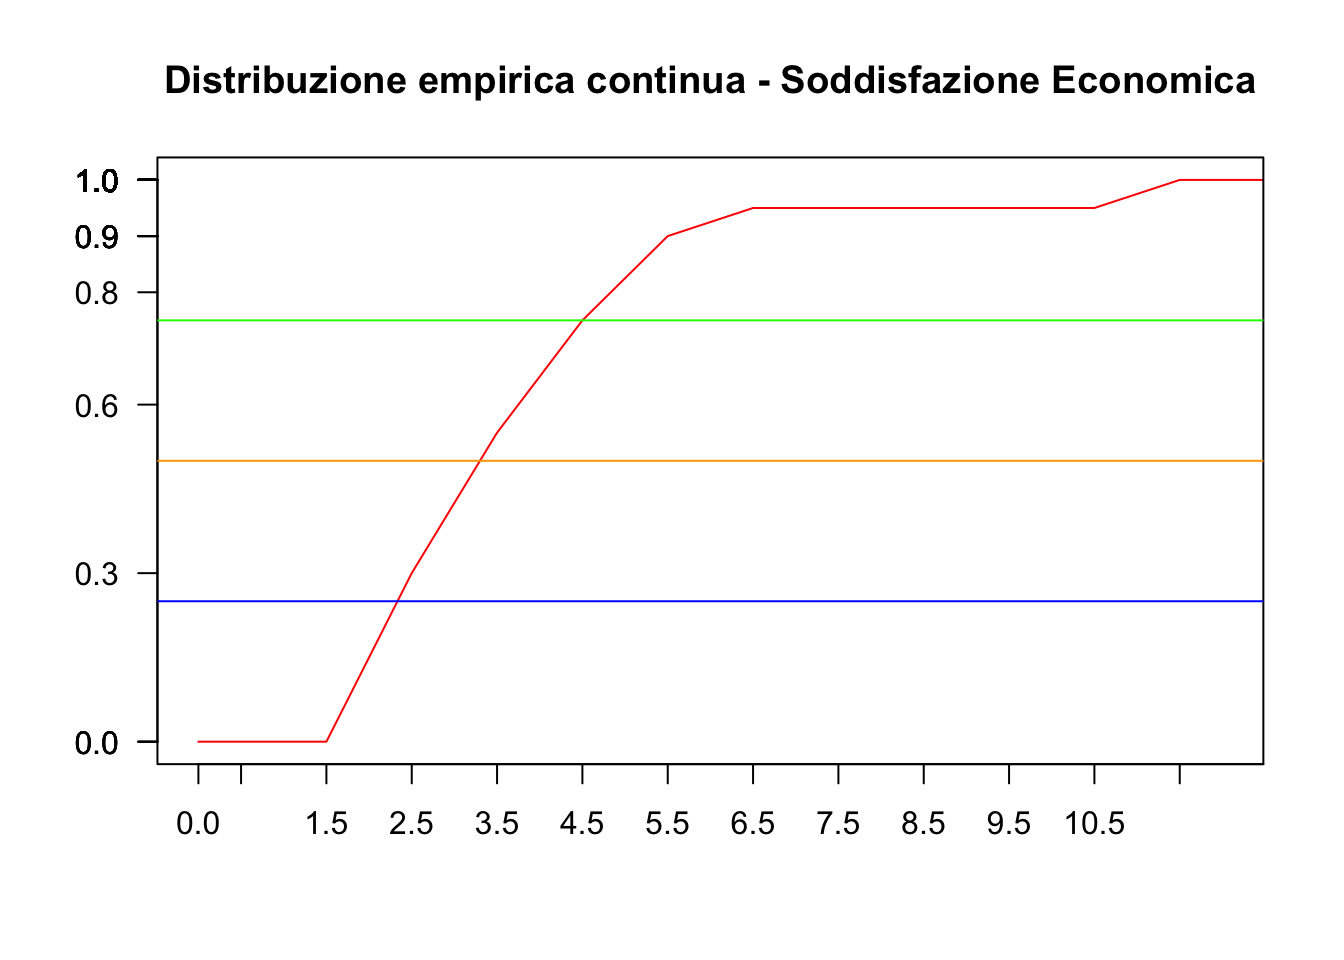
\includegraphics{statistics-project_files/figure-latex/distribuzione-quartili-1-1} 

}

\caption{Distribuzione empirica continua e quartili - Soddisfazione Economica}\label{fig:distribuzione-quartili-1}
\end{figure}

\begin{figure}

{\centering 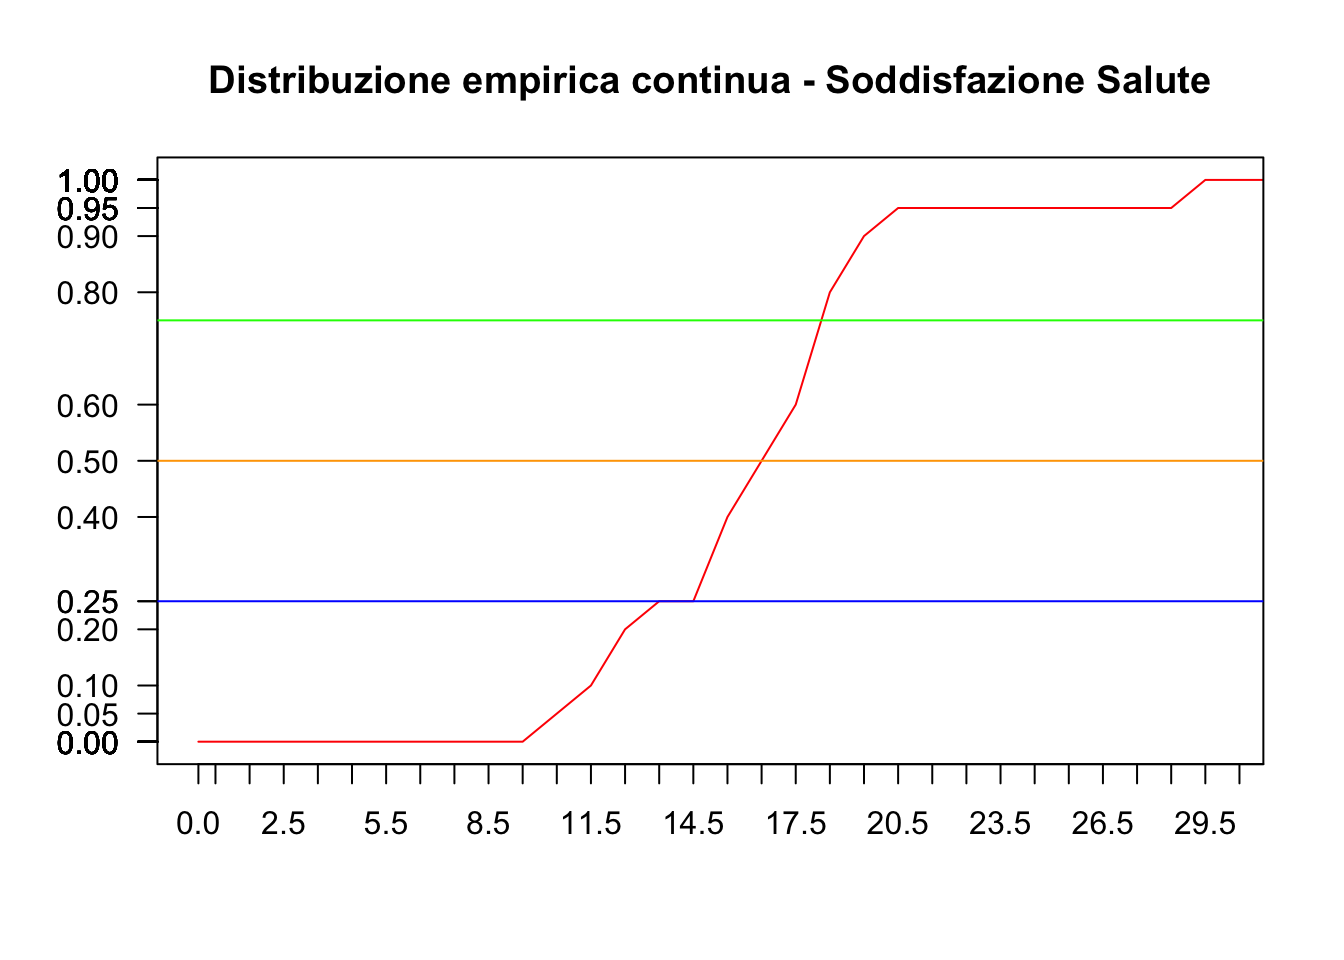
\includegraphics{statistics-project_files/figure-latex/distribuzione-quartili-2-1} 

}

\caption{Distribuzione empirica continua e quartili - Soddisfazione Salute}\label{fig:distribuzione-quartili-2}
\end{figure}

\begin{figure}

{\centering 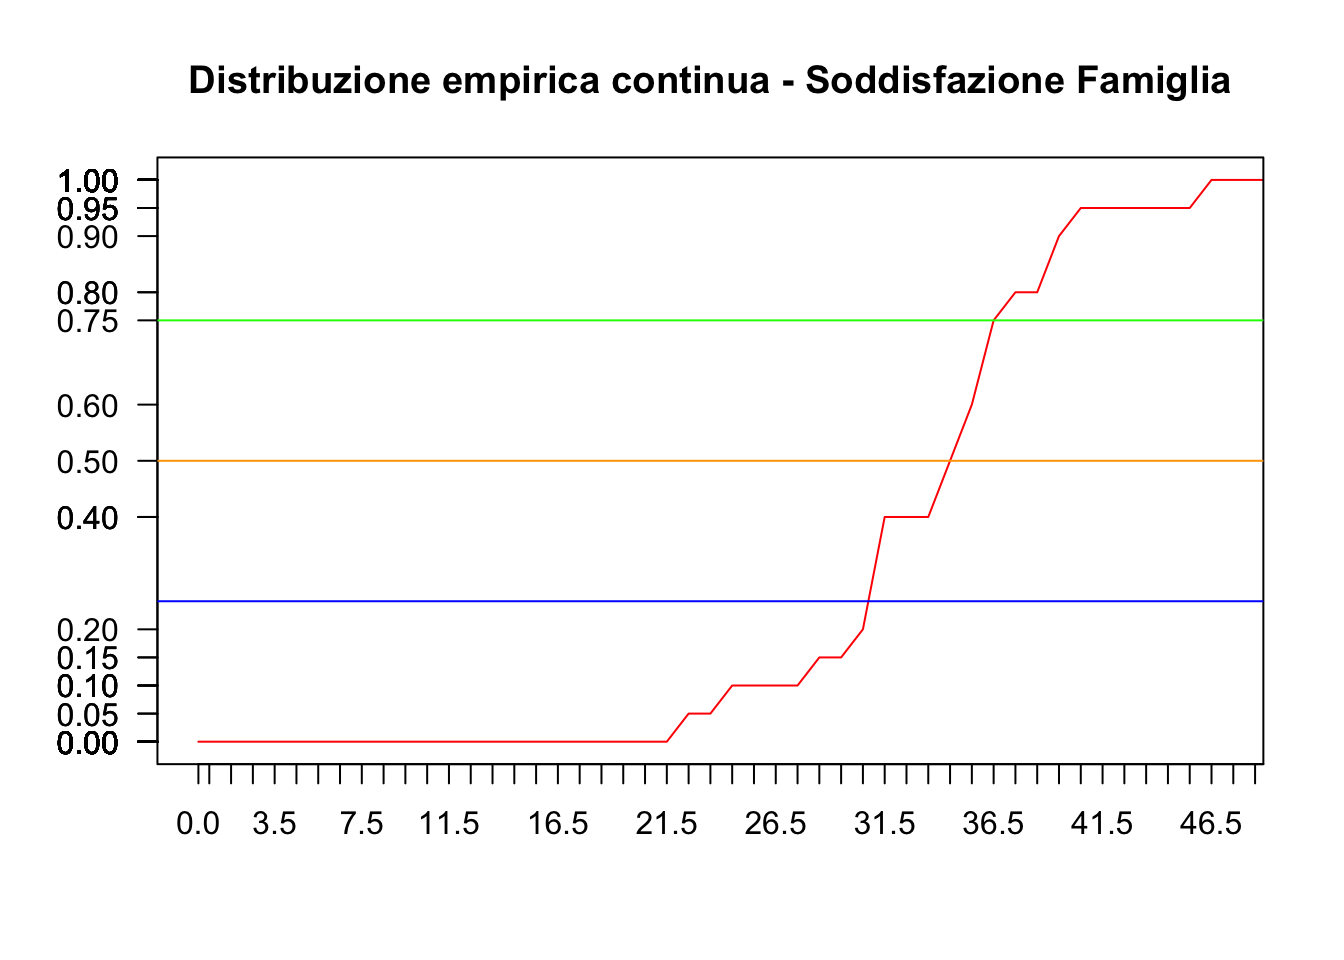
\includegraphics{statistics-project_files/figure-latex/distribuzione-quartili-3-1} 

}

\caption{Distribuzione empirica continua e quartili - Soddisfazione Famiglia}\label{fig:distribuzione-quartili-3}
\end{figure}

\begin{figure}

{\centering 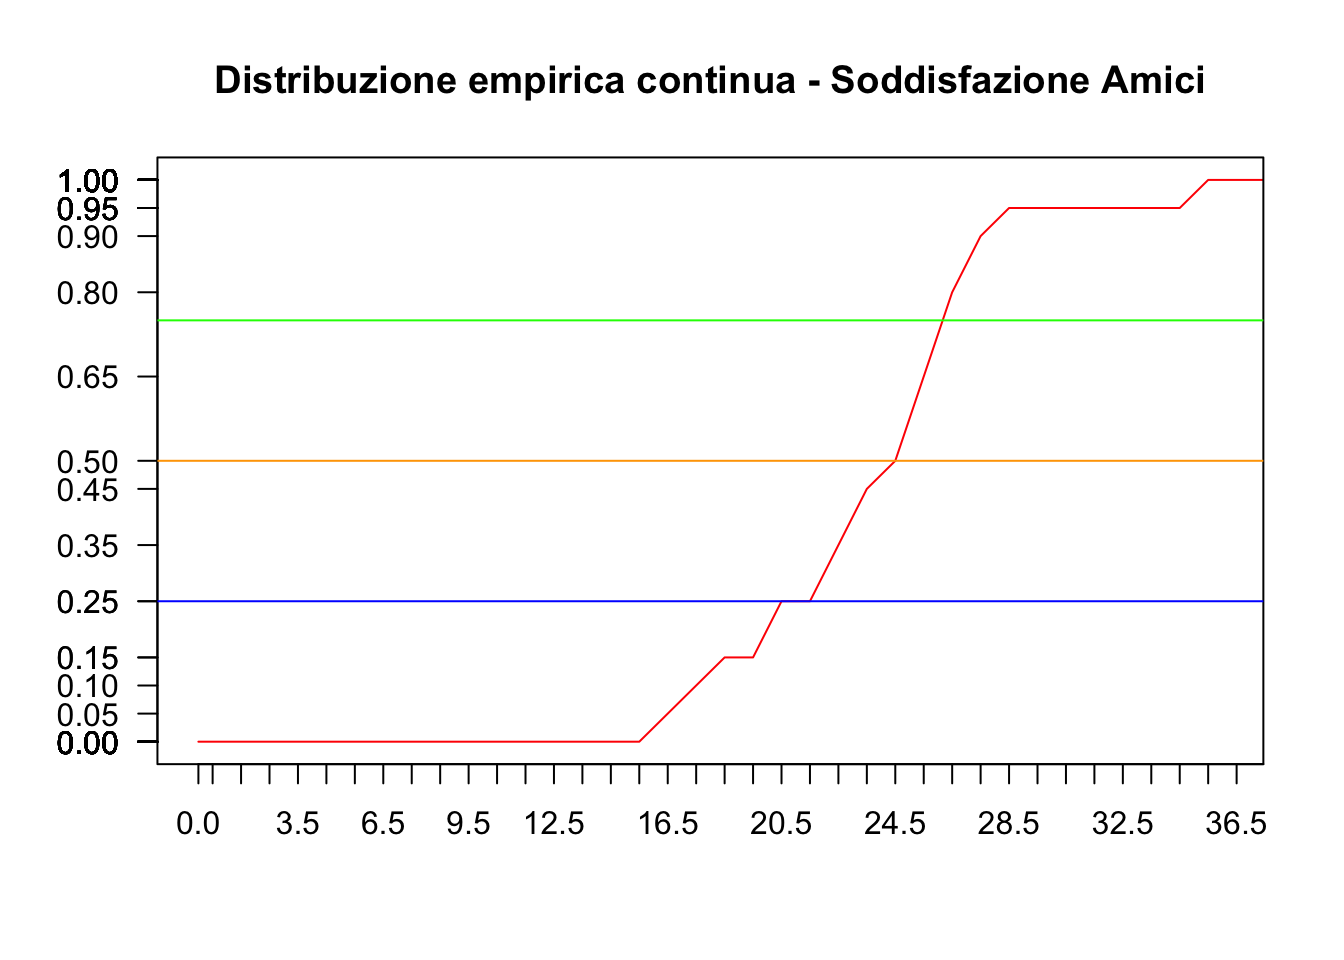
\includegraphics{statistics-project_files/figure-latex/distribuzione-quartili-4-1} 

}

\caption{Distribuzione empirica continua e quartili - Soddisfazione Amici}\label{fig:distribuzione-quartili-4}
\end{figure}

\begin{figure}

{\centering 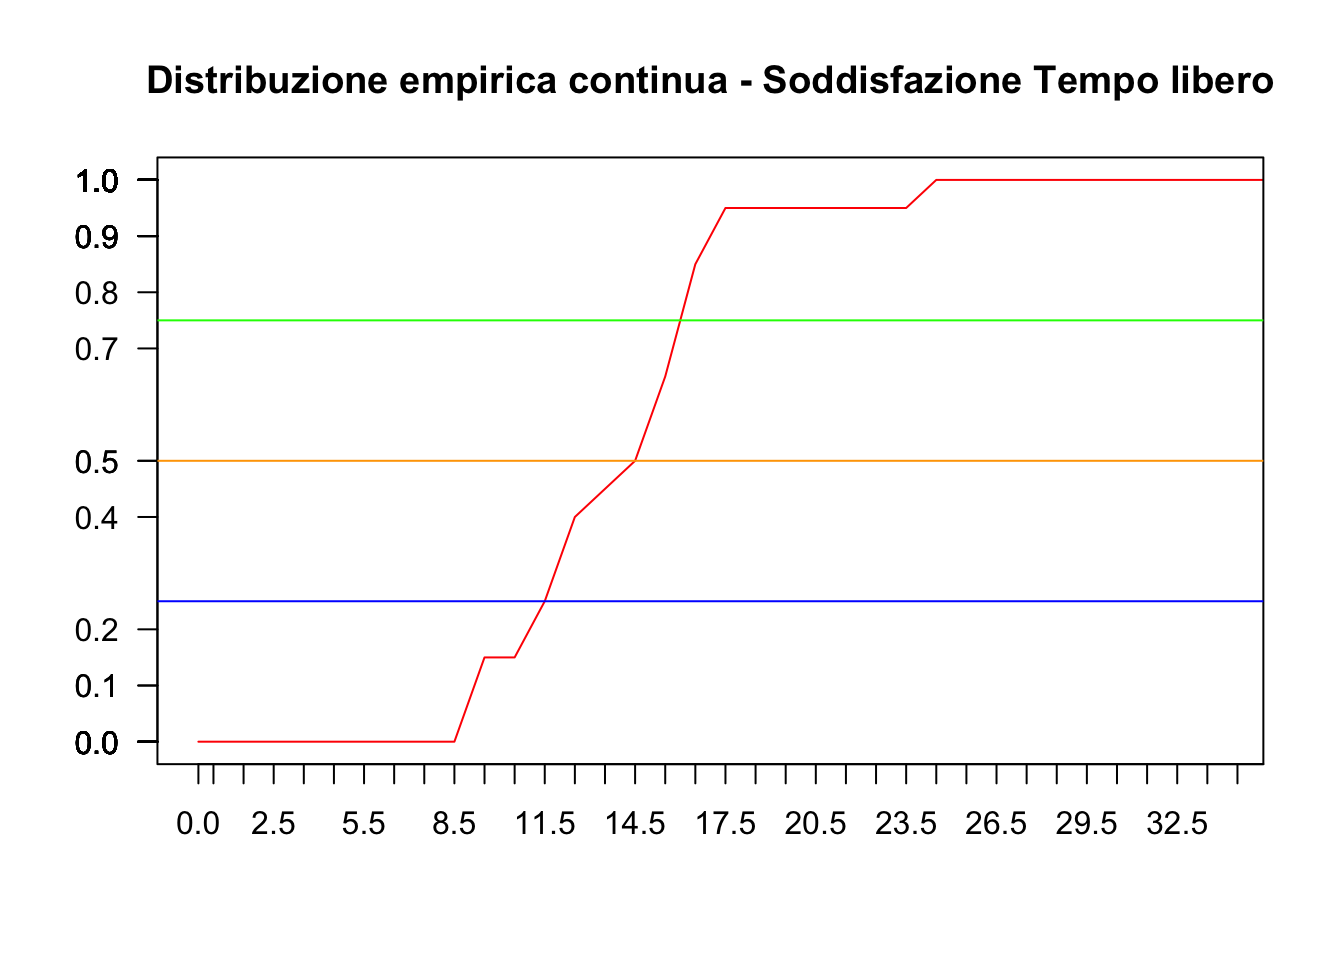
\includegraphics{statistics-project_files/figure-latex/distribuzione-quartili-5-1} 

}

\caption{Distribuzione empirica continua e quartili - Soddisfazione Tempo libero}\label{fig:distribuzione-quartili-5}
\end{figure}

\chapter{Indici di dispersione}\label{indici-di-dispersione}

Gli indici di dispersione sono indici di sintesi che descrivono quanto
un valore è distante da un indice centrale. Gli indici di dispersione
considerati nel seguito sono la varianza campionaria, la deviazione
standard campionaria e il coefficiente di variazione.

\section{Varianza campionaria}\label{varianza-campionaria}

La varianza campionaria fornisce una misura di quanto i valori si
discostano quadraticamente dalla media campionaria.

Formalmente dato un campione \(x_1,...,x_n\), la varianza campionaria
\(s^2\) è definita con la quantità
\[s^2=\frac{1}{n-1} \sum_{i=1}^{n}(x_1-\overline{x})^2\]

Ne consegue che se i valori del campione sono tutti uguali la varianza
campionaria è nulla, altrimenti il valore della varianza campionaria è
tanto più grande quando più i dati si discostano dalla media.

Il seguente codice permette di computare la varianza campionaria per
ogni caratteristica del data set. I risultati sono mostrati nella
tabella \ref{tab:varianza-campionaria}.

\begin{Shaded}
\begin{Highlighting}[]
\NormalTok{varianze <-}\StringTok{ }\KeywordTok{sapply}\NormalTok{(df, var)}
\end{Highlighting}
\end{Shaded}

Dai valori ottenuti si può notare che la variabilità maggiore si ottiene
nella soddisfazione in famiglia seguita da quella con gli amici, della
salute, del tempo libero, e infine economica.

\begin{table}

\caption{\label{tab:varianza-campionaria}Varianze campionarie}
\centering
\begin{tabular}[t]{l|l}
\hline
Caratteristica & Varianza campionaria\\
\hline
Economica & 4.42673684210526\\
\hline
Salute & 16.3402894736842\\
\hline
Famiglia & 30.3045\\
\hline
Amici & 19.5072631578947\\
\hline
Tempo libero & 12.4192368421053\\
\hline
\end{tabular}
\end{table}

\section{Deviazione standard
campionaria}\label{deviazione-standard-campionaria}

La deviazione standard campionaria detta anche scarto quadratico medio
campionario è definita come la radice quadrata della varianza
campionaria.

\[s = \sqrt{s^2}\]

Da notare che la deviazione standard campionaria ha le stesse unità di
misura del campione.

Il seguente codice permette di computare la deviazione standard
campionaria per ogni caratteristica del data set. I risultati sono
mostrati nella tabella \ref{tab:deviazione-standard-campionaria}.

\begin{Shaded}
\begin{Highlighting}[]
\NormalTok{deviazioniStandard <-}\StringTok{ }\KeywordTok{sapply}\NormalTok{(df, sd)}
\end{Highlighting}
\end{Shaded}

Per la deviazione standard campionaria le considerazioni sui risultati
sono analoghe a quelle della varianza campionaria.

\begin{table}

\caption{\label{tab:deviazione-standard-campionaria}Deviazione standard campionarie}
\centering
\begin{tabular}[t]{l|l}
\hline
Caratteristica & Deviazione standard campionaria\\
\hline
Economica & 2.10398118862913\\
\hline
Salute & 4.04231239189702\\
\hline
Famiglia & 5.50495231586978\\
\hline
Amici & 4.41670274728725\\
\hline
Tempo libero & 3.52409376182094\\
\hline
\end{tabular}
\end{table}

\section{Coefficiente di variazione}\label{coefficiente-di-variazione}

Il coefficiente di variazione è definito come il rapporto tra la
deviazione standard campionaria e il valore assoluto della media
campionaria. Essendo un numero puro, cioè adimensionale, può essere
utilizzato per confrontare le varianze di campioni con unità di misura
diverse o con differenti range di variazione. Dove con range di
variazione si intende la differenza tra il massimo e il minimo nel
campione. Inoltre va notato che il coefficiente di variazione può essere
calcolato solo se la media campionaria non è nulla.

Il seguente codice permette di calcolare il range di variazione per ogni
caratteristica. I risultati sono mostrati nella tabella
\ref{tab:range-variazione}.

\begin{Shaded}
\begin{Highlighting}[]
\NormalTok{range <-}\StringTok{ }\KeywordTok{sapply}\NormalTok{(df, max) }\OperatorTok{-}\StringTok{ }\KeywordTok{sapply}\NormalTok{(df, min)}
\end{Highlighting}
\end{Shaded}

Possiamo osservare che il range di variazione maggiore è relativo alla
soddisfazione in famiglia seguita dalla soddisfazione con gli amici,
salute, tempo libero e per ultimo quella economica.

\begin{table}

\caption{\label{tab:range-variazione}Range di variazione}
\centering
\begin{tabular}[t]{l|l}
\hline
Caratteristica & Range di variazione\\
\hline
Economica & 9.1\\
\hline
Salute & 18.5\\
\hline
Famiglia & 24.2\\
\hline
Amici & 19\\
\hline
Tempo libero & 14.6\\
\hline
\end{tabular}
\end{table}

Il seguente codice permette di calcolare il coefficiente di variazione
per ogni caratteristica. I valori sono mostrati nella tabella
\ref{tab:coefficiente-variazione}.

\begin{Shaded}
\begin{Highlighting}[]
\NormalTok{cv <-}\StringTok{ }\ControlFlowTok{function}\NormalTok{(x) \{}
  \KeywordTok{sd}\NormalTok{(x) }\OperatorTok{/}\StringTok{ }\KeywordTok{abs}\NormalTok{(}\KeywordTok{mean}\NormalTok{(x))}
\NormalTok{\}}
\NormalTok{coeffVariazione <-}\StringTok{ }\KeywordTok{sapply}\NormalTok{(df, cv)}
\end{Highlighting}
\end{Shaded}

Il coefficiente di variazione maggiore si ottiene con la soddisfazione
economica, seguita da quella per il tempo libero, per la salute, per gli
amici e infine per la famiglia.

\begin{table}

\caption{\label{tab:coefficiente-variazione}Coefficiente di variazione}
\centering
\begin{tabular}[t]{l|l}
\hline
Caratteristica & Coefficiente di variazione\\
\hline
Economica & 0.56256181514148\\
\hline
Salute & 0.245957553507577\\
\hline
Famiglia & 0.163424441617034\\
\hline
Amici & 0.187069154904161\\
\hline
Tempo libero & 0.252895138989662\\
\hline
\end{tabular}
\end{table}

\chapter{Correlazioni}\label{correlazioni}

In questo capitolo l'attenzione verrà posta sulle relazioni tra le
caratteristiche del data set. Le relazioni possono essere descritte
visivamente tramite diagrammi di dispersione o tramite una misura
quantitativa detta covarianza campionaria.

\section{Diagrammi si dispersione}\label{diagrammi-si-dispersione}

I diagrammi di dispersione detti anche scatterplot sono rappresentazioni
grafiche della correlazione tra variabili.

Dato un campione bivariato \((x_i, y_i)\) per \(i=1,...n\)
rappresentante \(n\) osservazioni delle variabili \((X, Y)\) il relativo
diagramma di dispersione consiste nel riportare i punti del campione su
un piano cartesiano dopo aver scelto una variabile indipendente e una
dipendente. Dalla visione del grafico è possibile intuire un'eventuale
regolarità tra i valori.

Il seguente codice permette di creare tutti gli scatterplot tra le
caratteristiche considerate. I diagrammi ottenuti sono mostrati in
figura \ref{fig:scatterplot}.

\begin{Shaded}
\begin{Highlighting}[]
\KeywordTok{pairs}\NormalTok{(df)}
\end{Highlighting}
\end{Shaded}

\begin{figure}

{\centering 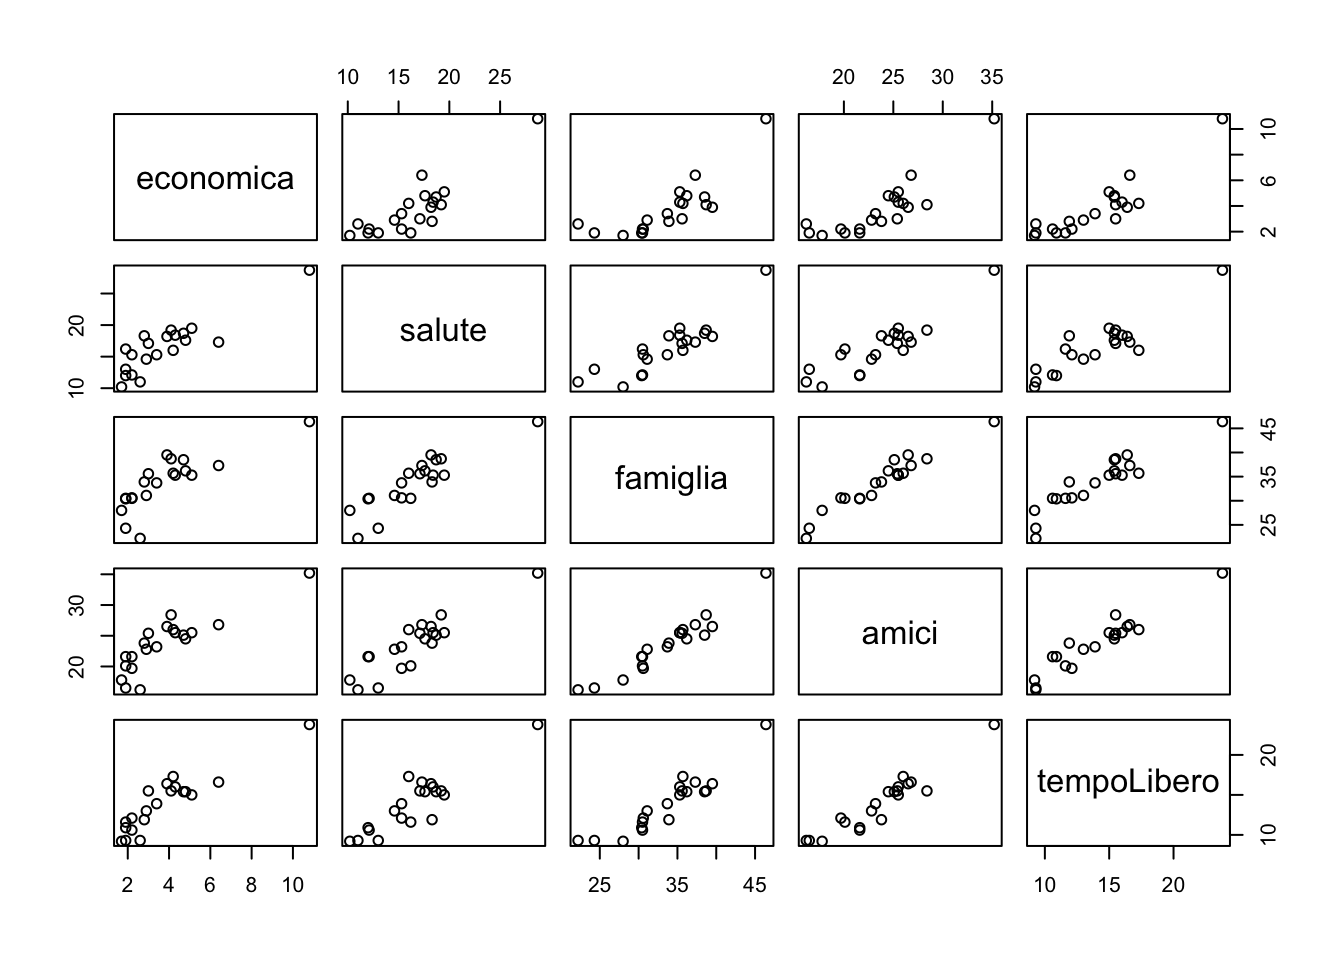
\includegraphics{statistics-project_files/figure-latex/scatterplot-1} 

}

\caption{Diagrammi si dispersione}\label{fig:scatterplot}
\end{figure}

In ogni diagramma la variabile indipendente è descritta dall'etichetta
presente nella stessa colonna del diagramma, mentre la variabile
dipendente è descritta dall'etichetta presente nella stessa riga del
diagramma. Dalla visualizzazione del grafico si può notare una
correlazione positiva tra tutte le caratteristiche prese a due a due.

\section{Covarianza campionaria}\label{covarianza-campionaria}

La covarianza campionaria consente di dare una misura quantitativa della
correlazione tra le variabili. Dato un campione bivariato \((x_i, y_i)\)
per \(i=1,...n\) la covarianza campionaria tra le variabili \(X\) e
\(Y\) è definita con il valore

\[C_{xy}=\frac{1}{n-1}\sum_{i=1}^{n}(x_i-\bar{x})(y_i-\bar{y})\]

Se la covarianza campionaria assume valore zero ne consegue che le
variabili non sono correlate, altrimenti all'aumentare del valore
assoluto della covarianza aumenta la correlazione. In particolare la
correlazione è positiva se il valore della covarianza è positivo,
negativa altrimenti.

Il seguente codice permette di calcolare la covarianza tra le
caratteristiche del data set prese a due a due. I risultati ottenuti
sono mostrati nella tabella \ref{tab:covarianze}. Da notare che la
correlazione tra le stesse variabili è uguale alla varianza tra le
variabili.

\begin{Shaded}
\begin{Highlighting}[]
\NormalTok{covarianze <-}\StringTok{ }\KeywordTok{cov}\NormalTok{(df)}
\end{Highlighting}
\end{Shaded}

\begin{table}

\caption{\label{tab:covarianze}Correlazioni}
\centering
\begin{tabular}[t]{l|r|r|r|r|r}
\hline
  & Economica & Salute & Famiglia & Amici & Tempo libero\\
\hline
Economica & 4.426737 & 7.399053 & 9.342211 & 7.977474 & 6.719579\\
\hline
Salute & 7.399053 & 16.340290 & 19.653710 & 15.970684 & 12.791868\\
\hline
Famiglia & 9.342211 & 19.653710 & 30.304500 & 23.511737 & 18.007395\\
\hline
Amici & 7.977474 & 15.970684 & 23.511737 & 19.507263 & 14.793316\\
\hline
Tempo libero & 6.719579 & 12.791868 & 18.007395 & 14.793316 & 12.419237\\
\hline
\end{tabular}
\end{table}

\section{Coefficiente di correlazione
campionario}\label{coefficiente-di-correlazione-campionario}

Il coefficiente di correlazione campionario è un coefficiente per
misurare in modo quantitativo la relazione lineare tra le variabili ed è
definito come \[r_{xy}=\frac{C_{xy}}{s_x s_y}\]

Assume valori compresi tra -1 e 1, in particolare assume valore zero nel
caso in cui le variabili non sono correlate, mentre all'aumentare del
valore assoluto del coefficiente aumenta la correlazione tra le
variabili. La correlazione è positiva se il segno del coefficiente è
positivo, negativa altrimenti.

Inoltre il coefficiente di correlazione campionario non fa distinzione
tra la variabile indipendente e la variabile dipendente.

Il seguente codice permette di calcolare il coefficiente di correlazione
campionario tra le caratteristiche del data set prese a due a due. I
risultati ottenuti sono mostrati nella tabella \ref{tab:correlazioni}.

\begin{Shaded}
\begin{Highlighting}[]
\NormalTok{correlazioni <-}\StringTok{ }\KeywordTok{cor}\NormalTok{(df)}
\end{Highlighting}
\end{Shaded}

\begin{table}

\caption{\label{tab:correlazioni}Correlazioni}
\centering
\begin{tabular}[t]{l|r|r|r|r|r}
\hline
  & Economica & Salute & Famiglia & Amici & Tempo libero\\
\hline
Economica & 1.0000000 & 0.8699702 & 0.8065926 & 0.8584705 & 0.9062599\\
\hline
Salute & 0.8699702 & 1.0000000 & 0.8832042 & 0.8945312 & 0.8979593\\
\hline
Famiglia & 0.8065926 & 0.8832042 & 1.0000000 & 0.9670145 & 0.9282177\\
\hline
Amici & 0.8584705 & 0.8945312 & 0.9670145 & 1.0000000 & 0.9504295\\
\hline
Tempo libero & 0.9062599 & 0.8979593 & 0.9282177 & 0.9504295 & 1.0000000\\
\hline
\end{tabular}
\end{table}

Il seguente codice permette di calcolare i valori della tabella
\ref{tab:correlazioni-ordinate} dove è mostrato il coefficiente di
correlazione campionario per tutte le caratteristiche prese a due a due
in ordine non crescente.

\begin{Shaded}
\begin{Highlighting}[]
\NormalTok{cc <-}\StringTok{ }\KeywordTok{numeric}\NormalTok{()}
\ControlFlowTok{for}\NormalTok{ (i }\ControlFlowTok{in} \DecValTok{1}\OperatorTok{:}\NormalTok{colCount) \{}
  \ControlFlowTok{for}\NormalTok{ (j }\ControlFlowTok{in} \DecValTok{1}\OperatorTok{:}\NormalTok{colCount) \{}
    \ControlFlowTok{if}\NormalTok{ (i }\OperatorTok{<}\StringTok{ }\NormalTok{j) \{}
\NormalTok{      value <-}\KeywordTok{array}\NormalTok{(correlazioni[i, j], }\KeywordTok{c}\NormalTok{(}\DecValTok{1}\NormalTok{, }\DecValTok{1}\NormalTok{))}
\NormalTok{      name <-}\StringTok{ }\KeywordTok{paste}\NormalTok{(}\KeywordTok{row.names}\NormalTok{(correlazioni)[i], }\StringTok{"-"}\NormalTok{,}
                    \KeywordTok{row.names}\NormalTok{(correlazioni)[j])}
      \KeywordTok{rownames}\NormalTok{(value) <-}\StringTok{ }\KeywordTok{c}\NormalTok{(name)}
\NormalTok{      cc <-}\StringTok{ }\KeywordTok{rbind}\NormalTok{(cc, value)}
\NormalTok{    \}}
\NormalTok{  \}}
\NormalTok{\}}
\NormalTok{lista.corr <-}\StringTok{ }\KeywordTok{as.matrix}\NormalTok{(cc[}\KeywordTok{order}\NormalTok{(cc[,}\DecValTok{1}\NormalTok{], }\DataTypeTok{decreasing =} \OtherTok{TRUE}\NormalTok{),])}
\end{Highlighting}
\end{Shaded}

Possiamo osservare che la correlazione maggiore si presenta tra la
soddisfazione in famiglia e la soddisfazione con gli amici. Mentre la
correlazione minore tra la soddisfazione in famiglia e quella economica.
Si nota inoltre che tutte le correlazioni sono positive.

\begin{table}

\caption{\label{tab:correlazioni-ordinate}Coefficiente di correlazione campionario}
\centering
\begin{tabular}[t]{l|r}
\hline
  & Coef. Correlazione\\
\hline
Famiglia - Amici & 0.9670145\\
\hline
Amici - Tempo libero & 0.9504295\\
\hline
Famiglia - Tempo libero & 0.9282177\\
\hline
Economica - Tempo libero & 0.9062599\\
\hline
Salute - Tempo libero & 0.8979593\\
\hline
Salute - Amici & 0.8945312\\
\hline
Salute - Famiglia & 0.8832042\\
\hline
Economica - Salute & 0.8699702\\
\hline
Economica - Amici & 0.8584705\\
\hline
Economica - Famiglia & 0.8065926\\
\hline
\end{tabular}
\end{table}

\section{Coefficiente di
determinazione}\label{coefficiente-di-determinazione}

Per determinare se il modello di regressione spiega i dati è utile
considerare il coefficiente di determinazione, anche chiamato r-square,
e definito con il valore
\[D^2=\frac{\sum_{i=1}^n(\hat{y}_i-\bar{y})^2}{\sum_{i=1}^n(y_i-\bar{y})^2}\]
Dove con \(\hat{y}_i\) e \(y_i\) sono rispettivamente è l'\(i\)-esimo
valore stimato e osservato, mentre \(\bar{y}\) è la media campionaria
dei valori osservati.

Il coefficiente di determinazione può essere anche visto come il
rapporto tra la varianza dei valori stimati e quella dei valori
osservati.

Se il coefficiente di determinazione assume valore zero vi è una
completa incapacità del modello di spiegare i valori, altrimenti
all'aumentare del valore del coefficiente di determinazione aumenta la
capacità del modello di spiegare i valori. Nel caso limite in cui il
coefficiente assume valore uno il modello di regressione spiega
perfettamente i valori.

\subsubsection{Coefficiente di determinazione nella regressione
lineare}\label{coefficiente-di-determinazione-nella-regressione-lineare}

Nella regressione lineare il coefficiente di determinazione è
equivalente al quadrato del coefficiente di determinazione
\[D^2=r_{xy}^2\]

Il seguente codice permette di calcolare il coefficiente di
determinazione per il modello lineare per tutte le caratteristiche prese
a due a due. I risultati sono mostrati nella tabella
\ref{tab:coeff-determinazione}.

\begin{Shaded}
\begin{Highlighting}[]
\NormalTok{coeffDeterminazione <-}\StringTok{ }\NormalTok{lista.corr }\OperatorTok{^}\StringTok{ }\DecValTok{2}
\end{Highlighting}
\end{Shaded}

Il coefficiente di determinazione minore è associato alle
caratteristiche soddisfazione economica e soddisfazione in famiglia con
un valore 0.6505916. Ne consegue che la regressione lineare non
approssima in modo soddisfacente i valori. Per tutte le altre
caratteristiche prese a due a due il modello lineare approssima i valori
con buona soddisfazione, infatti il coefficiente di determinazione è
maggiore di 0.7369715, ottenendo un massimo pari a 0.935117 tra la
soddisfazione per la famiglia e quella per gli amici.

\begin{table}

\caption{\label{tab:coeff-determinazione}Coefficienti di determinazione}
\centering
\begin{tabular}[t]{l|r}
\hline
  & Coef. determinazione\\
\hline
Famiglia - Amici & 0.9351170\\
\hline
Amici - Tempo libero & 0.9033162\\
\hline
Famiglia - Tempo libero & 0.8615882\\
\hline
Economica - Tempo libero & 0.8213070\\
\hline
Salute - Tempo libero & 0.8063309\\
\hline
Salute - Amici & 0.8001860\\
\hline
Salute - Famiglia & 0.7800496\\
\hline
Economica - Salute & 0.7568482\\
\hline
Economica - Amici & 0.7369715\\
\hline
Economica - Famiglia & 0.6505916\\
\hline
\end{tabular}
\end{table}

Nel seguito verrà mostrato il modello di regressione lineare e relativa
analisi tra la soddisfazione per la famiglia e quella per gli amici.
Verrà inoltre anche mostrato come la soddisfazione economica e la
soddisfazione per la salute influiscono sulla soddisfazione nel tempo
libero tramite una regressione lineare multipla. Infine verrà mostrato
un modello di regressione non lineare per la correlazione tra la
soddisfazione economica e quella in famiglia.

\section{Regressione lineare}\label{regressione-lineare}

Il modello di regressione lineare è un metodo di stima che mira a
trovare la retta che meglio interpola la nuvola dei punti.

I valori del coefficiente angolare \(\beta\) e dell'intercetta
\(\alpha\) vengono calcolati tramite il metodo dei minimi quadrati e
hanno valori pari a
\[\beta = \frac{s_y}{s_x} r_{xy} \quad  \alpha=\overline{y}-\beta\overline{x}\]

Il seguente codice calcola il modello lineare per la variabile
indipendente associata alla soddisfazione per la famiglia e la variabile
dipendente associata alla soddisfazione per gli amici. L'intercetta, il
coefficiente angolare e il coefficiente di determinazione per tale
modello sono mostrati nella tabella \ref{tab:modello-lineare-dati}

\begin{Shaded}
\begin{Highlighting}[]
\NormalTok{y <-}\StringTok{ }\NormalTok{df}\OperatorTok{$}\NormalTok{amici}
\NormalTok{x <-}\StringTok{ }\NormalTok{df}\OperatorTok{$}\NormalTok{famiglia}
\NormalTok{modello <-}\StringTok{ }\KeywordTok{lm}\NormalTok{(y}\OperatorTok{~}\NormalTok{x)}
\NormalTok{intercetta <-}\StringTok{ }\NormalTok{modello}\OperatorTok{$}\NormalTok{coefficients[[}\DecValTok{1}\NormalTok{]]}
\NormalTok{coeffAngolare <-}\StringTok{ }\NormalTok{modello}\OperatorTok{$}\NormalTok{coefficients[[}\DecValTok{2}\NormalTok{]]}
\NormalTok{coeffDeterminazione <-}\StringTok{ }\KeywordTok{summary}\NormalTok{(modello)}\OperatorTok{$}\NormalTok{r.squared}
\end{Highlighting}
\end{Shaded}

Poiché il coefficiente angolare è positivo ne consegue che la retta di
regressione è una retta crescente.

\begin{table}

\caption{\label{tab:modello-lineare-dati}Dati modello lineare}
\centering
\begin{tabular}[t]{r|r|r}
\hline
Intercetta & Coef. Angolare & Coef. Determinazione\\
\hline
-2.524497 & 0.7758497 & 0.935117\\
\hline
\end{tabular}
\end{table}

Invece il diagramma del modello di regressione è disegnato con il
seguente codice ed è mostrato in figura
\ref{fig:modello-lineare-scatterplot}

\begin{Shaded}
\begin{Highlighting}[]
\KeywordTok{plot}\NormalTok{(x, y, }\DataTypeTok{xlab =} \StringTok{"Soddisfazione Famiglia"}\NormalTok{, }
     \DataTypeTok{ylab =} \StringTok{"Soddisfazione Amici"}\NormalTok{, }
     \DataTypeTok{main =} \StringTok{"Regressione lineare semplice"}\NormalTok{)}
\KeywordTok{abline}\NormalTok{(modello, }\DataTypeTok{col=}\StringTok{"blue"}\NormalTok{)  }
\end{Highlighting}
\end{Shaded}

\begin{figure}

{\centering 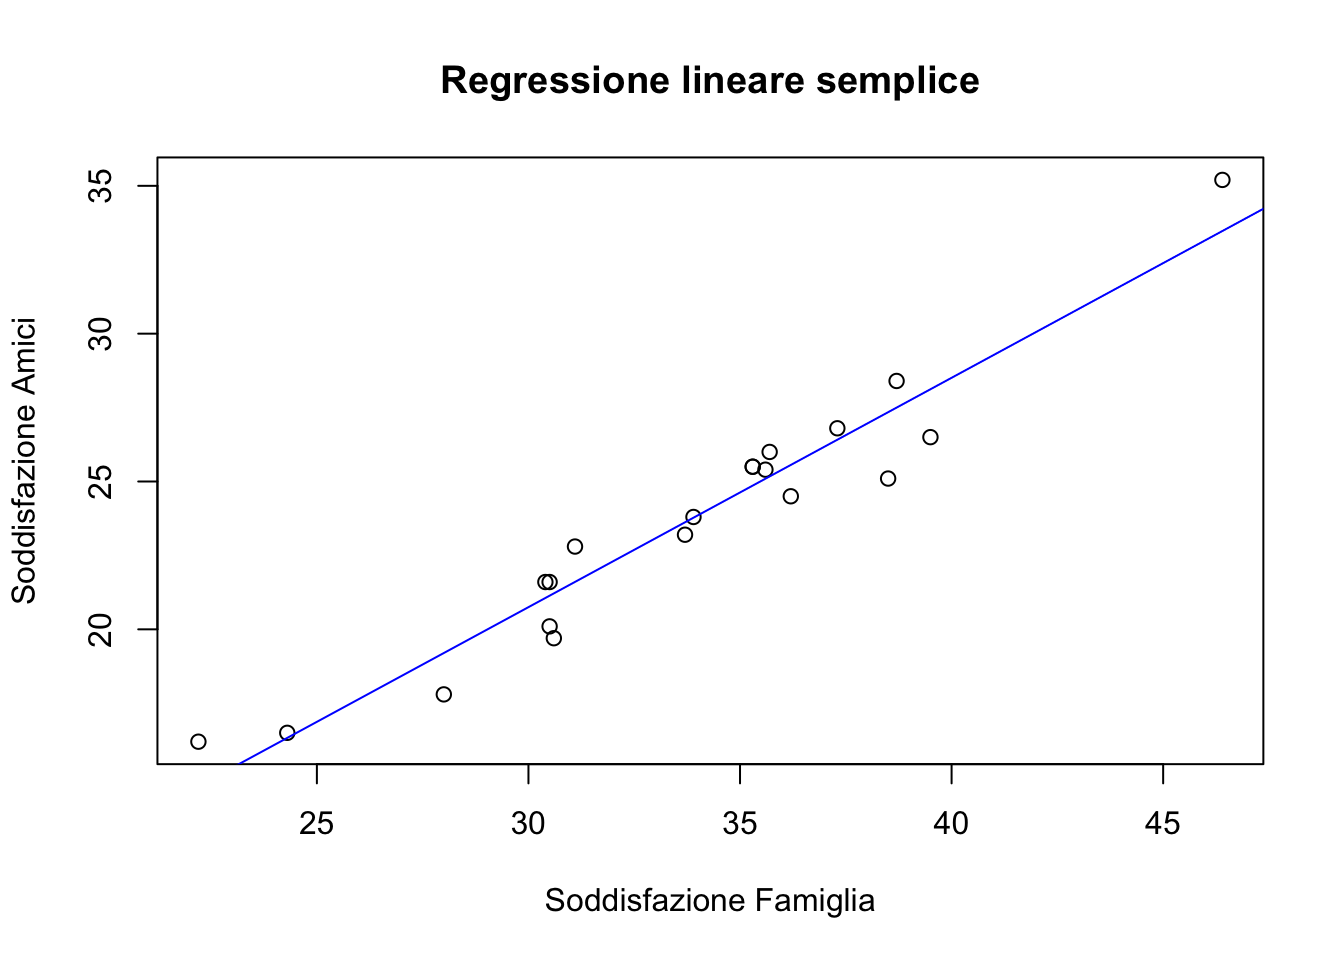
\includegraphics{statistics-project_files/figure-latex/modello-lineare-scatterplot-1} 

}

\caption{Diagramma di dispersione}\label{fig:modello-lineare-scatterplot}
\end{figure}

La stima dei valori tramite il modello lineare può differire dai valori
osservati nel caso in cui i punti non sono tutti sulla retta
interpolante. Con residuo si definisce la differenza tra il valore
osservato e il valore stimato.

Può essere notato che la media campionaria dei residui è nulla, di
conseguenza gli scostamenti positivi e negativi si compensano. Inoltre
la media campionaria dei valori stimati è uguale alla media campionaria
dei valori osservati.

Il seguente codice permette di calcolare i valori stimati, i residui, e
i residui standardizzati. I risultati sono mostrati nella tabella
\ref{tab:modello-lineare-residui}.\\
Inoltre vengono calcolate alcune statistiche sui residui: la media
campionaria, la varianza campionaria e deviazione standard campionaria.
Non può essere calcolato il coefficiente di variazione poiché la media
dei residui è zero. I risultati sono mostrati nella tabella
\ref{tab:modello-lineare-residui-statistiche}.

\begin{Shaded}
\begin{Highlighting}[]
\NormalTok{osservati <-}\StringTok{ }\NormalTok{y}
\NormalTok{stime <-}\StringTok{ }\KeywordTok{fitted}\NormalTok{(modello)}
\NormalTok{residui <-}\KeywordTok{resid}\NormalTok{(modello)}
\NormalTok{residui.standard <-}\StringTok{ }\NormalTok{residui }\OperatorTok{/}\StringTok{ }\KeywordTok{sd}\NormalTok{(residui)}

\NormalTok{mediaResidui <-}\StringTok{ }\KeywordTok{mean}\NormalTok{(residui)}
\NormalTok{varianzaResidui <-}\StringTok{ }\KeywordTok{var}\NormalTok{(residui)}
\NormalTok{deviazioneStandardResidui <-}\StringTok{ }\KeywordTok{sd}\NormalTok{(residui)}
\end{Highlighting}
\end{Shaded}

\begin{table}

\caption{\label{tab:modello-lineare-residui}Residui}
\centering
\begin{tabular}[t]{r|r|r|r}
\hline
Osservati & Stimati & Residui & Residui standardizzati\\
\hline
24.5 & 25.56126 & -1.0612620 & -0.9433199\\
\hline
25.5 & 24.86300 & 0.6370028 & 0.5662102\\
\hline
26.5 & 28.12157 & -1.6215659 & -1.4413552\\
\hline
25.5 & 24.86300 & 0.6370028 & 0.5662102\\
\hline
35.2 & 33.47493 & 1.7250712 & 1.5333576\\
\hline
25.1 & 27.34572 & -2.2457162 & -1.9961414\\
\hline
26.8 & 26.41470 & 0.3853034 & 0.3424832\\
\hline
28.4 & 27.50089 & 0.8991138 & 0.7991919\\
\hline
25.4 & 25.09575 & 0.3042478 & 0.2704356\\
\hline
26.0 & 25.17334 & 0.8266629 & 0.7347927\\
\hline
23.2 & 23.62164 & -0.4216377 & -0.3747796\\
\hline
22.8 & 21.60443 & 1.1955714 & 1.0627031\\
\hline
23.8 & 23.77681 & 0.0231923 & 0.0206149\\
\hline
19.7 & 21.21650 & -1.5165037 & -1.3479690\\
\hline
16.5 & 16.32865 & 0.1713493 & 0.1523066\\
\hline
16.2 & 14.69937 & 1.5006337 & 1.3338626\\
\hline
21.6 & 21.13892 & 0.4610813 & 0.4098396\\
\hline
17.8 & 19.19929 & -1.3992945 & -1.2437857\\
\hline
20.1 & 21.13892 & -1.0389187 & -0.9234598\\
\hline
21.6 & 21.06133 & 0.5386662 & 0.4788022\\
\hline
\end{tabular}
\end{table}

\begin{table}

\caption{\label{tab:modello-lineare-residui-statistiche}Statistiche Residui}
\centering
\begin{tabular}[t]{r|r|r}
\hline
Media & Varianza & Deviazione Standard\\
\hline
0 & 1.265689 & 1.125029\\
\hline
\end{tabular}
\end{table}

Una visualizzazione grafica dei residui sulla retta di regressione è
mostrata in figura
\ref{fig:modello-lineare-regressione-residui-standard} mentre un
diagramma mostrante i valori dei residui rispetto ai valori stimati è
mostrato in figura \ref{fig:modello-lineare-diagramma-residui-standard}.
In quest'ultimo grafico la retta orizzontale rappresenta la media
campionaria dei residui di valore zero.

\begin{figure}

{\centering 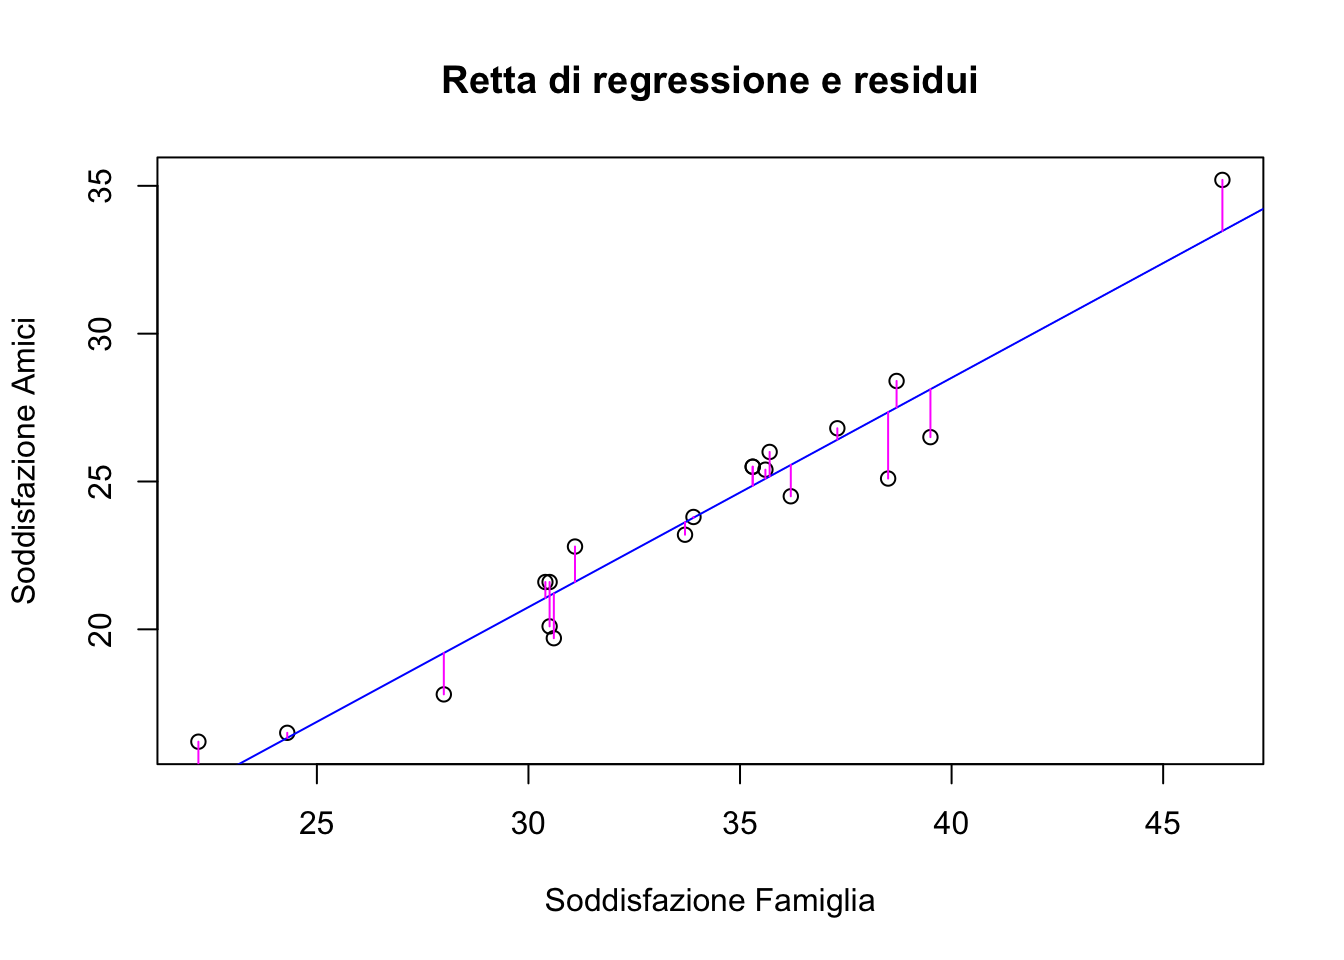
\includegraphics{statistics-project_files/figure-latex/modello-lineare-regressione-residui-standard-1} 

}

\caption{Diagramma di dispersione}\label{fig:modello-lineare-regressione-residui-standard}
\end{figure}

\begin{figure}

{\centering 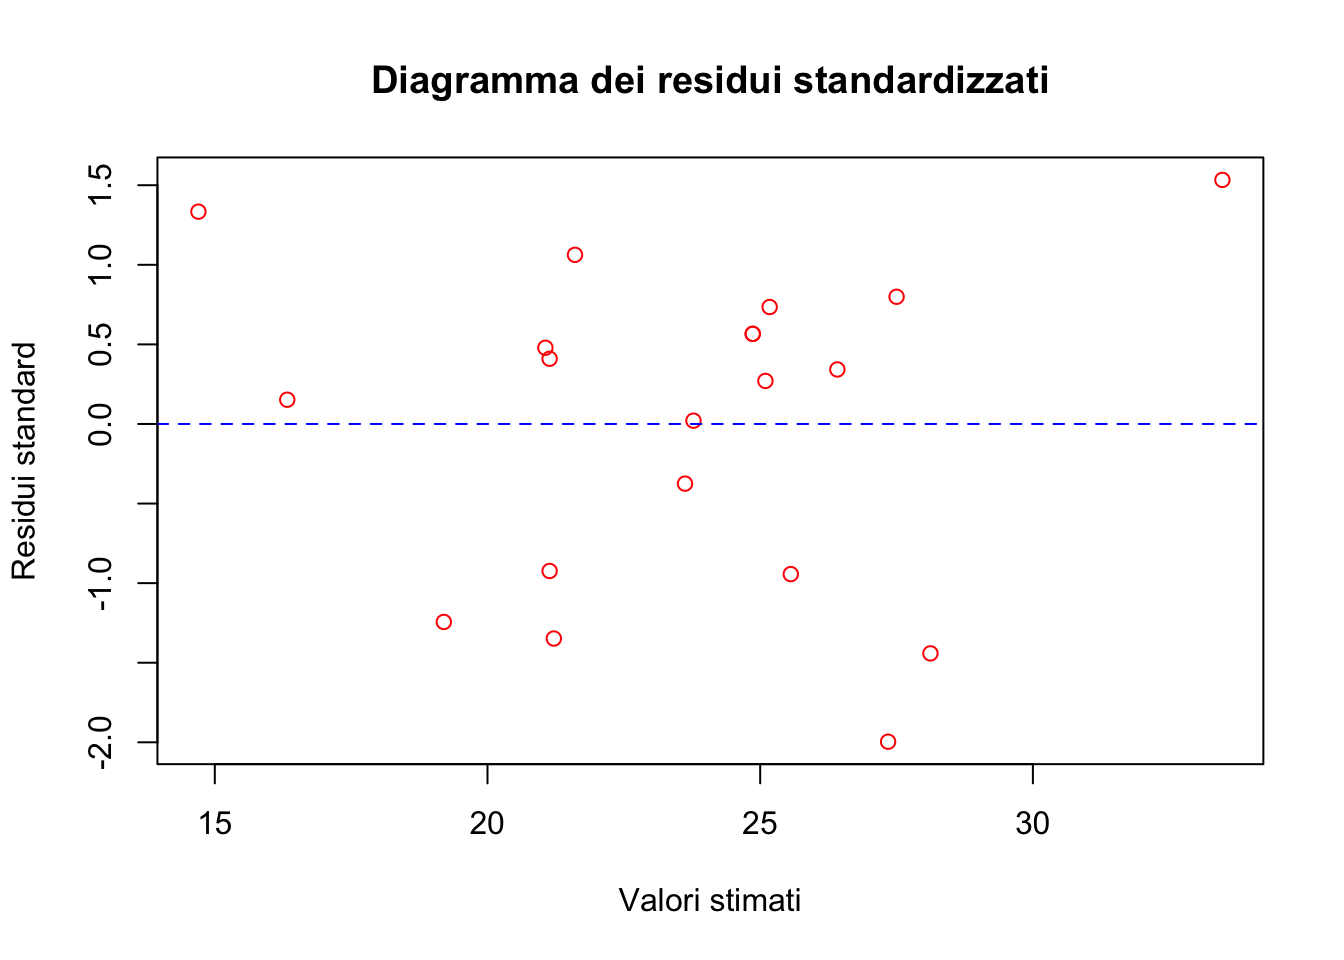
\includegraphics{statistics-project_files/figure-latex/modello-lineare-diagramma-residui-standard-1} 

}

\caption{Diagramma di dispersione}\label{fig:modello-lineare-diagramma-residui-standard}
\end{figure}

Come è possibile notare alcuni residui si discostano in modo maggiore
degli altri dal valore medio influenzando l'andamento della retta
interpolante

\section{Regressione lineare
multipla}\label{regressione-lineare-multipla}

In questo paragrafo si desidera analizzare quanto la soddisfazione
economica e la soddisfazione per la salute influiscono sulla
soddisfazione nel tempo libero. La correlazione tra più variabili viene
analizzata per mezzo del modello di regressione lineare multivariato. Il
quale è descritto dalla retta
\[Y = \alpha = \beta_1 X_1 +\dots + \beta_p X_p\] dove \(\alpha\) è
l'intercetta e i \(\beta_i\) per \(i=1,..,p\) sono i regressori.
L'intercetta e i regressori sono calcolati con il metodo dei minimi
quadrati.

Il seguente codice calcola il modello lineare multivariato per le
variabili indipendenti associate alla soddisfazione economica e alla
soddisfazione per la salute e la variabile dipendente associata alla
soddisfazione nel tempo libero. I parametri e il coefficiente di
determinazione per tale modello sono mostrati nella tabella
\ref{tab:modello-lineare-multivariato-dati}

\begin{Shaded}
\begin{Highlighting}[]
\NormalTok{y <-}\StringTok{ }\NormalTok{df}\OperatorTok{$}\NormalTok{tempoLibero}

\NormalTok{x1 <-}\StringTok{ }\NormalTok{df}\OperatorTok{$}\NormalTok{economica}
\NormalTok{x2 <-}\StringTok{ }\NormalTok{df}\OperatorTok{$}\NormalTok{salute}
\NormalTok{modello <-}\StringTok{ }\KeywordTok{lm}\NormalTok{(y}\OperatorTok{~}\NormalTok{x1}\OperatorTok{+}\NormalTok{x2)}

\NormalTok{alfa <-}\StringTok{ }\NormalTok{modello}\OperatorTok{$}\NormalTok{coefficients[[}\DecValTok{1}\NormalTok{]]}
\NormalTok{beta1 <-}\StringTok{ }\NormalTok{modello}\OperatorTok{$}\NormalTok{coefficients[[}\DecValTok{2}\NormalTok{]]}
\NormalTok{beta2 <-}\StringTok{ }\NormalTok{modello}\OperatorTok{$}\NormalTok{coefficients[[}\DecValTok{3}\NormalTok{]]}
\NormalTok{coeffDeterminazione <-}\StringTok{ }\KeywordTok{summary}\NormalTok{(modello)}\OperatorTok{$}\NormalTok{r.squared}
\end{Highlighting}
\end{Shaded}

Poiché entrambi i regressori sono positivi ne consegue che sia la
soddisfazione economica sia quella della salute hanno un effetto
positivo sulla soddisfazione nel tempo libero.

Inoltre poiché il valore del coefficiente di determinazione assume
valore 0.870655 ne consegue che il modello di regressione lineare
multipla spiega in modo soddisfacente i valori.

\begin{table}

\caption{\label{tab:modello-lineare-multivariato-dati}Dati modello lineare}
\centering
\begin{tabular}[t]{r|r|r|r}
\hline
α & β1 & β2 & Coef. Determinazione\\
\hline
4.258195 & 0.8614965 & 0.3927476 & 0.870655\\
\hline
\end{tabular}
\end{table}

Il seguente codice permette di calcolare i valori stimati, i residui, e
i residui standardizzati. I risultati sono mostrati nella tabella
\ref{tab:modello-lineare-multivariato-residui}.\\
Inoltre vengono calcolate alcune statistiche sui residui: la media
campionaria, la varianza campionaria e la deviazione standard
campionaria. I risultati sono mostrati nella tabella
\ref{tab:modello-lineare-multivariato-statistiche}.

\begin{Shaded}
\begin{Highlighting}[]
\NormalTok{osservati <-}\StringTok{ }\NormalTok{y}
\NormalTok{stime <-}\StringTok{ }\KeywordTok{fitted}\NormalTok{(modello)}
\NormalTok{residui <-}\KeywordTok{resid}\NormalTok{(modello)}
\NormalTok{residui.standard <-}\StringTok{ }\NormalTok{residui }\OperatorTok{/}\StringTok{ }\KeywordTok{sd}\NormalTok{(residui)}

\NormalTok{mediaResidui <-}\StringTok{ }\KeywordTok{mean}\NormalTok{(residui)}
\NormalTok{varianzaResidui <-}\StringTok{ }\KeywordTok{var}\NormalTok{(residui)}
\NormalTok{deviazioneStandardResidui <-}\StringTok{ }\KeywordTok{sd}\NormalTok{(residui)}
\end{Highlighting}
\end{Shaded}

\begin{table}

\caption{\label{tab:modello-lineare-multivariato-residui}Residui}
\centering
\begin{tabular}[t]{r|r|r|r}
\hline
Osservati & Stimati & Residui & Residui standardizzati\\
\hline
15.4 & 15.305737 & 0.0942627 & 0.0743734\\
\hline
15.0 & 16.310407 & -1.3104068 & -1.0339125\\
\hline
16.4 & 14.766039 & 1.6339610 & 1.2891971\\
\hline
16.0 & 15.189187 & 0.8108128 & 0.6397323\\
\hline
23.8 & 24.834215 & -1.0342154 & -0.8159972\\
\hline
15.4 & 15.651610 & -0.2516101 & -0.1985207\\
\hline
16.6 & 16.566308 & 0.0336925 & 0.0265834\\
\hline
15.5 & 15.331086 & 0.1689140 & 0.1332734\\
\hline
15.5 & 13.558670 & 1.9413302 & 1.5317119\\
\hline
17.3 & 14.160443 & 3.1395568 & 2.4771141\\
\hline
13.9 & 13.196323 & 0.7036774 & 0.5552023\\
\hline
13.0 & 12.490651 & 0.5093490 & 0.4018770\\
\hline
11.9 & 13.857668 & -1.9576676 & -1.5446021\\
\hline
12.1 & 12.162527 & -0.0625268 & -0.0493337\\
\hline
9.3 & 11.000758 & -1.7007582 & -1.3419003\\
\hline
9.3 & 10.818311 & -1.5183105 & -1.1979488\\
\hline
10.6 & 10.905734 & -0.3057343 & -0.2412247\\
\hline
9.2 & 9.728765 & -0.5287655 & -0.4171966\\
\hline
11.6 & 12.257551 & -0.6575507 & -0.5188083\\
\hline
10.9 & 10.608011 & 0.2919894 & 0.2303800\\
\hline
\end{tabular}
\end{table}

\begin{table}

\caption{\label{tab:modello-lineare-multivariato-statistiche}Statistiche Residui}
\centering
\begin{tabular}[t]{r|r|r}
\hline
Media & Varianza & Deviazione Standard\\
\hline
0 & 1.606367 & 1.267425\\
\hline
\end{tabular}
\end{table}

Infine una visualizzazione grafica dei residui rispetto ai valori
stimati è mostrata in figura
\ref{fig:modello-lineare-multivariato-diagramma-residui-standard}.

\begin{figure}

{\centering 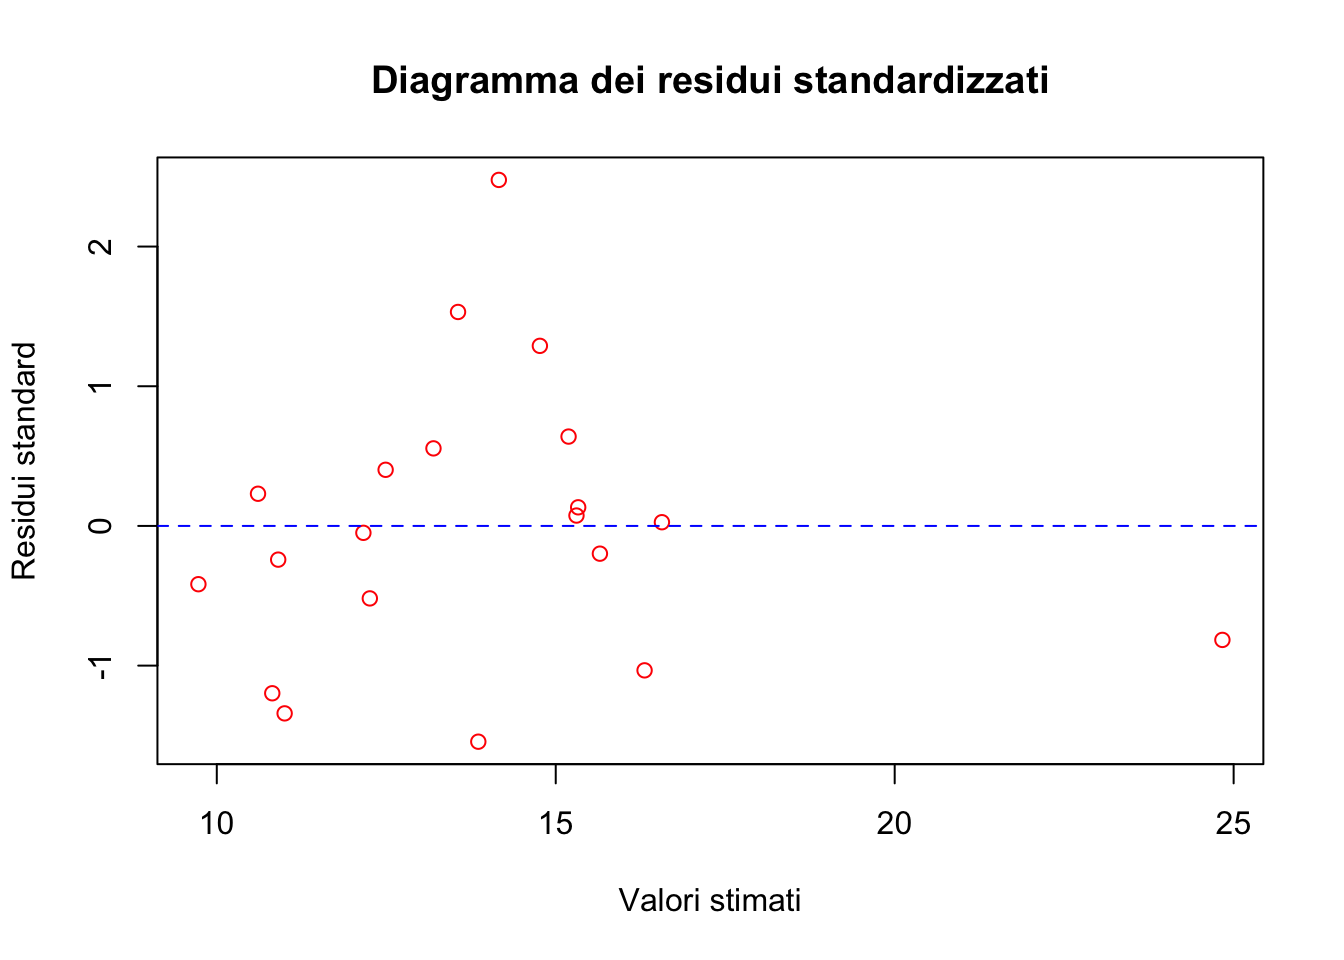
\includegraphics{statistics-project_files/figure-latex/modello-lineare-multivariato-diagramma-residui-standard-1} 

}

\caption{Diagramma di dispersione}\label{fig:modello-lineare-multivariato-diagramma-residui-standard}
\end{figure}

\section{Regressione polinomiale}\label{regressione-polinomiale}

Come visto precedentemente il modello lineare non riesce a spiegare la
correlazione tra la soddisfazione in famiglia e la soddisfazione
economica. Nel seguito verrà utilizzato la regressione polinomiale per
modellare la correlazione tra queste due caratteristiche.

Al modello di regressione polinomiale è associata la curva
\[Y = \alpha + \beta X + \gamma X^2\]

e per stimare i parametri \(\alpha\), \(\beta\) e \(\gamma\) si utilizza
la regressione lineare multipla
\[Y = \alpha + \beta X_1 + \gamma X_2^2\]

con i regressori \(X_1=X\) e \(X_2=X^2\).

Il seguente codice calcola il modello polinomiale per la variabile
indipendente associata alla soddisfazione in famiglia e la variabile
dipendente associata alla soddisfazione economica. I parametri
\(\alpha\), \(\beta\) e \(\gamma\) e il coefficiente di determinazione
per tale modello sono mostrati nella tabella
\ref{tab:modello-polinomiale-dati}

\begin{Shaded}
\begin{Highlighting}[]
\NormalTok{y <-}\StringTok{ }\NormalTok{df}\OperatorTok{$}\NormalTok{economica}
\NormalTok{x <-}\StringTok{ }\NormalTok{df}\OperatorTok{$}\NormalTok{famiglia}
\NormalTok{modello <-}\StringTok{ }\KeywordTok{lm}\NormalTok{(y}\OperatorTok{~}\NormalTok{x }\OperatorTok{+}\StringTok{ }\KeywordTok{I}\NormalTok{(x }\OperatorTok{^}\StringTok{ }\DecValTok{2}\NormalTok{))}
\NormalTok{alpha <-}\StringTok{ }\NormalTok{modello}\OperatorTok{$}\NormalTok{coefficients[[}\DecValTok{1}\NormalTok{]]}
\NormalTok{beta <-}\StringTok{ }\NormalTok{modello}\OperatorTok{$}\NormalTok{coefficients[[}\DecValTok{2}\NormalTok{]]}
\NormalTok{gamma <-}\StringTok{ }\NormalTok{modello}\OperatorTok{$}\NormalTok{coefficients[[}\DecValTok{3}\NormalTok{]]}
\NormalTok{coeffDeterminazione <-}\StringTok{ }\KeywordTok{summary}\NormalTok{(modello)}\OperatorTok{$}\NormalTok{r.squared}
\end{Highlighting}
\end{Shaded}

\begin{table}

\caption{\label{tab:modello-polinomiale-dati}Dati modello polinomiale}
\centering
\begin{tabular}[t]{r|r|r|r}
\hline
α & β & ɣ & Coef. Determinazione\\
\hline
16.06647 & -1.078837 & 0.0206401 & 0.8469753\\
\hline
\end{tabular}
\end{table}

Essendo il coefficiente di determinazione pari a 0.8469753 ne consegue
che il modello spiega i valori in modo soddisfacente.

Invece il diagramma del modello di regressione è disegnato con il
seguente codice ed è mostrato in figura
\ref{fig:modello-polinomiale-scatterplot}

\begin{Shaded}
\begin{Highlighting}[]
\KeywordTok{plot}\NormalTok{(x, y, }\DataTypeTok{xlab =} \StringTok{"Soddisfazione Famiglia"}\NormalTok{, }
     \DataTypeTok{ylab =} \StringTok{"Soddisfazione Economica"}\NormalTok{,}
     \DataTypeTok{main =} \StringTok{"Regressione polinomiale"}\NormalTok{)}
\KeywordTok{curve}\NormalTok{(alpha}\OperatorTok{+}\NormalTok{beta}\OperatorTok{*}\NormalTok{x}\OperatorTok{+}\NormalTok{gamma}\OperatorTok{*}\NormalTok{(x}\OperatorTok{^}\DecValTok{2}\NormalTok{) ,}\DataTypeTok{from=}\DecValTok{20}\NormalTok{,}\DataTypeTok{to=}\DecValTok{50}\NormalTok{, }\DataTypeTok{col=}\StringTok{"red"}\NormalTok{, }\DataTypeTok{add =} \OtherTok{TRUE}\NormalTok{)}
\end{Highlighting}
\end{Shaded}

\begin{figure}

{\centering 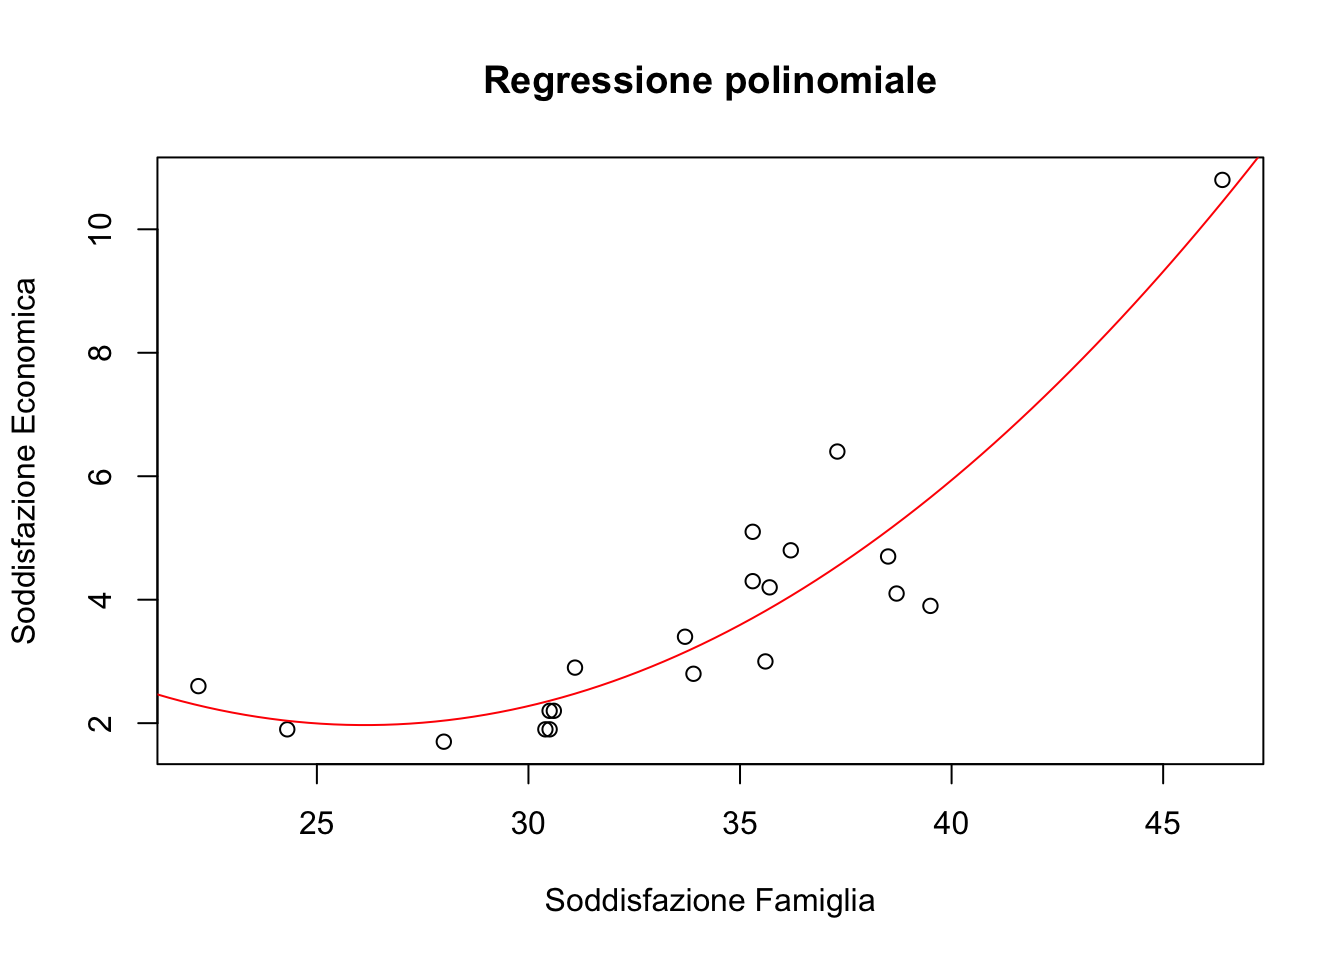
\includegraphics{statistics-project_files/figure-latex/modello-polinomiale-scatterplot-1} 

}

\caption{Diagramma di dispersione}\label{fig:modello-polinomiale-scatterplot}
\end{figure}

Il seguente codice permette di calcolare i valori stimati, i residui, e
i residui standardizzati. I risultati sono mostrati nella tabella
\ref{tab:modello-polinomiale-residui}.\\
Inoltre vengono calcolate alcune statistiche sui residui: la media
campionaria, la varianza campionaria e deviazione standard campionaria.
I risultati sono mostrati nella tabella
\ref{tab:modello-polinomiale-residui-statistiche}.

\begin{Shaded}
\begin{Highlighting}[]
\NormalTok{osservati <-}\StringTok{ }\NormalTok{y}
\NormalTok{stime <-}\StringTok{ }\KeywordTok{fitted}\NormalTok{(modello)}
\NormalTok{residui <-}\KeywordTok{resid}\NormalTok{(modello)}
\NormalTok{residui.standard <-}\StringTok{ }\NormalTok{residui }\OperatorTok{/}\StringTok{ }\KeywordTok{sd}\NormalTok{(residui)}

\NormalTok{mediaResidui <-}\StringTok{ }\KeywordTok{mean}\NormalTok{(residui)}
\NormalTok{varianzaResidui <-}\StringTok{ }\KeywordTok{var}\NormalTok{(residui)}
\NormalTok{deviazioneStandardResidui <-}\StringTok{ }\KeywordTok{sd}\NormalTok{(residui)}
\end{Highlighting}
\end{Shaded}

\begin{table}

\caption{\label{tab:modello-polinomiale-residui}Residui}
\centering
\begin{tabular}[t]{r|r|r|r}
\hline
Osservati & Stimati & Residui & Residui standardizzati\\
\hline
4.8 & 4.060237 & 0.7397631 & 0.8988145\\
\hline
5.1 & 3.702997 & 1.3970026 & 1.6973626\\
\hline
3.9 & 5.656187 & -1.7561871 & -2.1337730\\
\hline
4.3 & 3.702997 & 0.5970026 & 0.7253600\\
\hline
10.8 & 10.445826 & 0.3541737 & 0.4303222\\
\hline
4.7 & 5.125094 & -0.4250935 & -0.5164900\\
\hline
6.4 & 4.542271 & 1.8577288 & 2.2571464\\
\hline
4.1 & 5.228010 & -1.1280098 & -1.3705356\\
\hline
3.0 & 3.818362 & -0.8183620 & -0.9943125\\
\hline
4.2 & 3.857642 & 0.3423575 & 0.4159654\\
\hline
3.4 & 3.150466 & 0.2495344 & 0.3031851\\
\hline
2.9 & 2.477992 & 0.4220084 & 0.5127416\\
\hline
2.8 & 3.213753 & -0.4137528 & -0.5027110\\
\hline
2.2 & 2.380662 & -0.1806618 & -0.2195047\\
\hline
1.9 & 2.038530 & -0.1385305 & -0.1683149\\
\hline
2.6 & 2.288579 & 0.3114214 & 0.3783781\\
\hline
2.2 & 2.362434 & -0.1624343 & -0.1973582\\
\hline
1.7 & 2.040907 & -0.3409067 & -0.4142027\\
\hline
1.9 & 2.362434 & -0.4624343 & -0.5618591\\
\hline
1.9 & 2.344620 & -0.4446196 & -0.5402142\\
\hline
\end{tabular}
\end{table}

\begin{table}

\caption{\label{tab:modello-polinomiale-residui-statistiche}Statistiche Residui}
\centering
\begin{tabular}[t]{r|r|r}
\hline
Media & Varianza & Deviazione Standard\\
\hline
0 & 0.6773999 & 0.8230431\\
\hline
\end{tabular}
\end{table}

Una visualizzazione grafica dei residui sulla retta di regressione è
mostrata in figura
\ref{fig:modello-polinomiale-regressione-residui-standard} mentre un
diagramma mostrante i valori dei residui rispetto ai valori stimati è
mostrato in figura
\ref{fig:modello-polinomiale-diagramma-residui-standard}.

\begin{figure}

{\centering 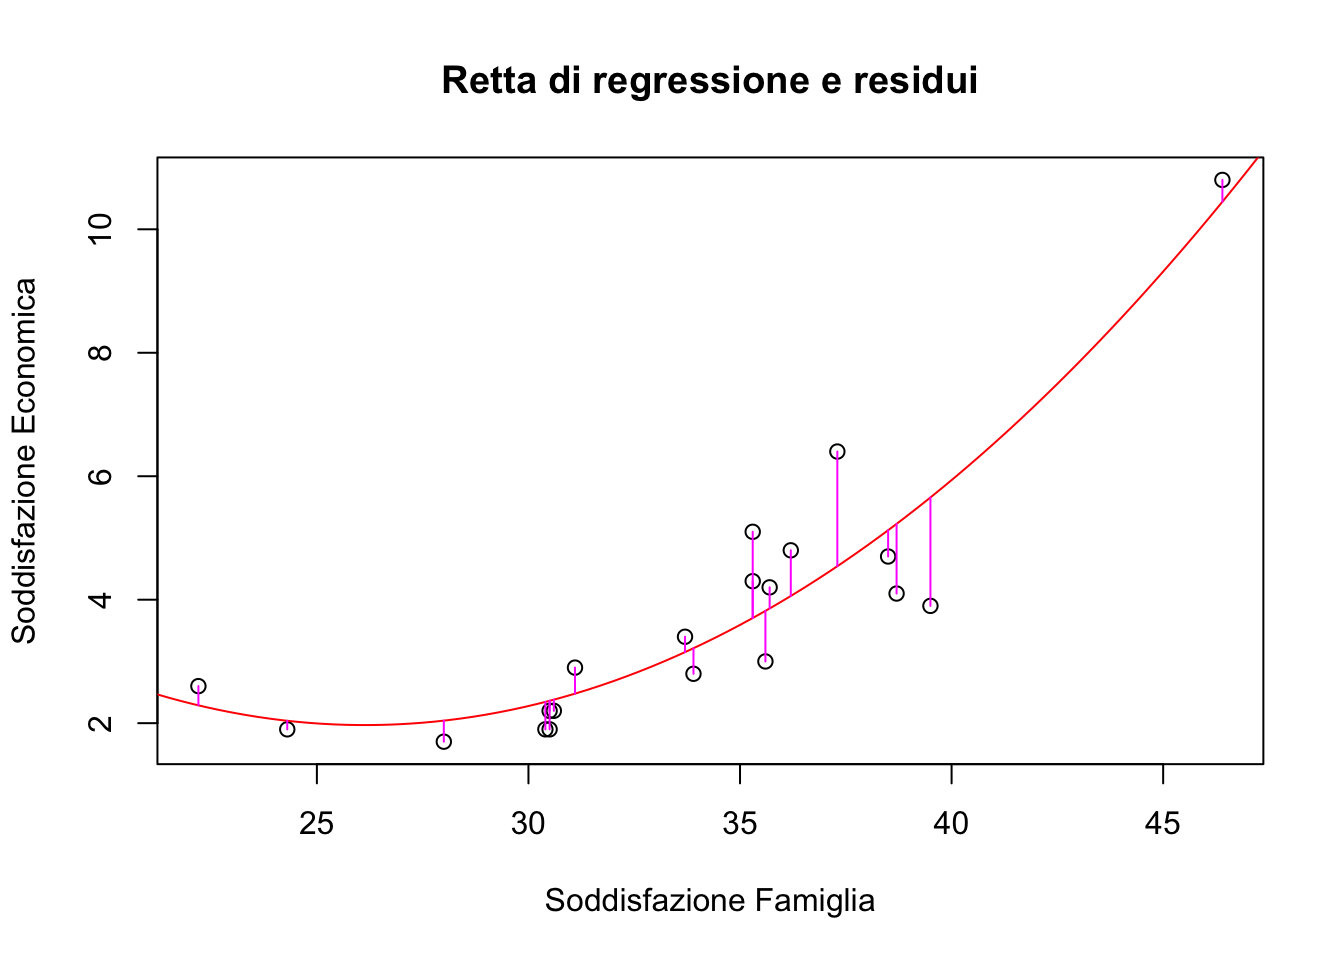
\includegraphics{statistics-project_files/figure-latex/modello-polinomiale-regressione-residui-standard-1} 

}

\caption{Diagramma di dispersione}\label{fig:modello-polinomiale-regressione-residui-standard}
\end{figure}

\begin{figure}

{\centering 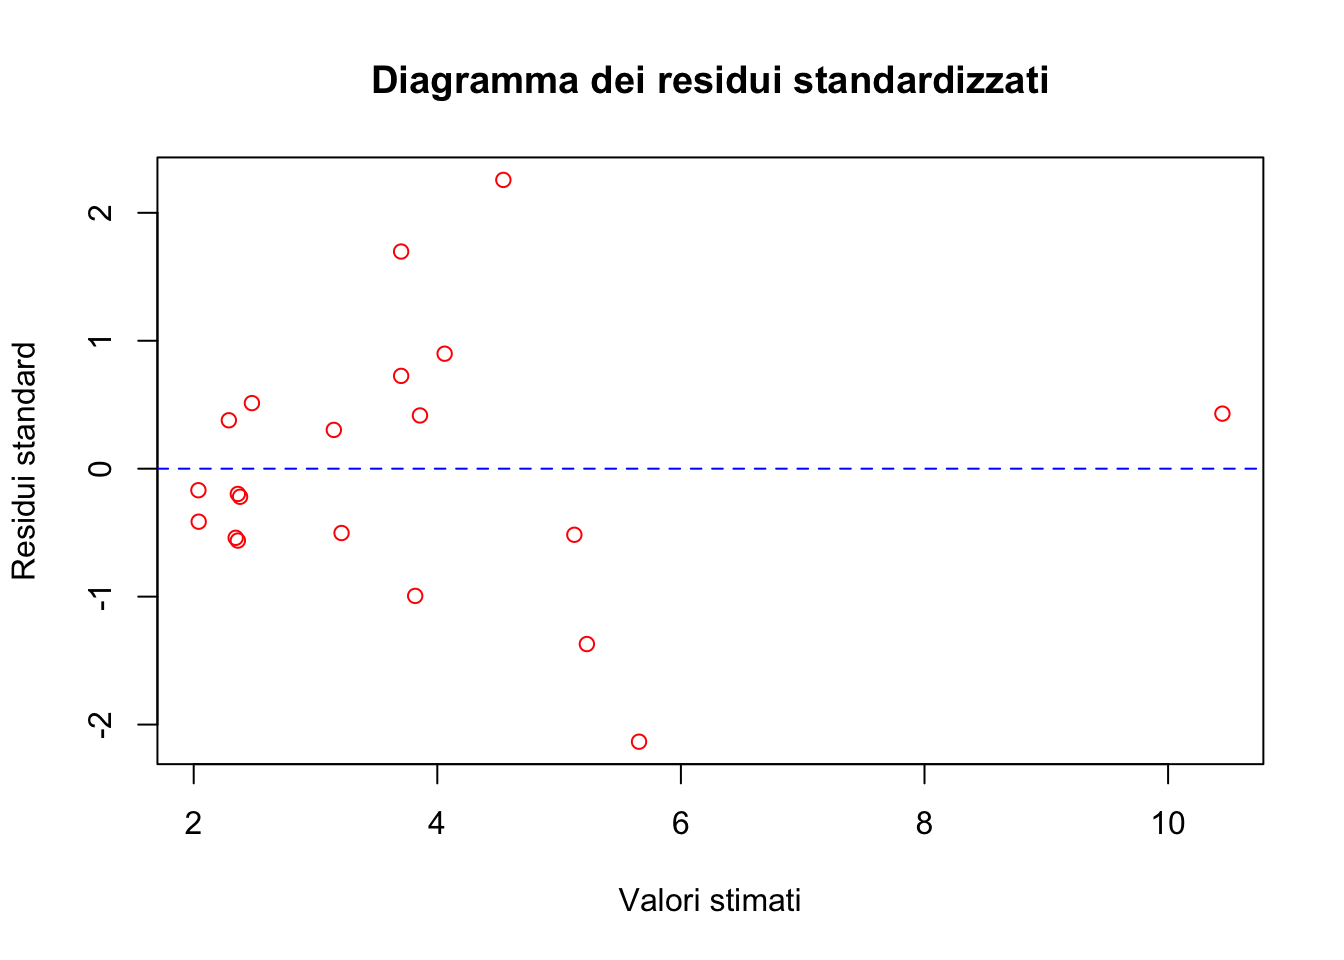
\includegraphics{statistics-project_files/figure-latex/modello-polinomiale-diagramma-residui-standard-1} 

}

\caption{Diagramma di dispersione}\label{fig:modello-polinomiale-diagramma-residui-standard}
\end{figure}

\chapter{Analisi dei cluster}\label{analisi-dei-cluster}

In questo capitolo verrà effettuata l'analisi dei cluster che ha come
obbiettivo il raggruppamento degli individui del campione in gruppi con
caratteristiche simili.

Poiché gli individui del nostro campione sono le regioni italiane
cercheremo di determinare dei gruppi costituiti da regioni aventi un
grado di associazione elevato, e aventi un grado di associazione basso
con le regioni presenti negli altri gruppi.

Per determinare quantitativamente la somiglianza tra gli individui è
possibile utilizzare misure di distanza o misure di similarità.

Essendo i metodi di enumerazione completa troppo costosi l'analisi dei
cluster sarà effettuata prima con metodi gerarchici agglomerativi e poi
con un metodo non gerarchico. I metodi gerarchici consentiranno di avere
una visione in termini di distanze e consentiranno di scegliere il
numero di cluster. Il metodo non gerarchico k-mean cercherà di
migliorare i risultati ottenuti precedentemente grazie alla
riallocazione degli individui tra i cluster.

Per ogni metodo gerarchico sarà mostrato anche il dendrogramma, un
grafico che riporta sull'asse delle ascisse gli individui e sull'asse
delle ordinate le distanze di aggregazione.

Con i metodi per cui è possibile verrà effettuata anche un'analisi con
lo screeplot. Lo screeplot è un grafico in cui sulle ordinate vengono
posti i numeri di gruppi che si possono ottenere con il metodo
gerarchico e sull'asse delle ascisse le distanze di aggregazione.
Calcolate le differenze tra le distanze di aggregazione per formare
\(k\) gruppi e \(k - 1\) gruppi per \(k = 2,..,n\) dove \(n\) è il
numero di individui, la procedura consiglia di scegliere il numero di
cluster pari a \(l\) se la distanza di aggregazione per formare \(l\)
gruppi e \(l - 1\) gruppi è la distanza più grande tra le distanze
possibili. Va notato che l'analisi dello screen plot non suggerisce
sempre il numero ottimale di cluster e che non è consigliabile usare il
metodo del centroide e della mediana in quanto le distanze di
agglomerazioni potrebbero essere non crescenti.

\section{Misure di distanza}\label{misure-di-distanza}

Dati due individui \(I_i\) e \(I_j\), e definito con \(X_i\) il vettore
delle caratteristiche dell'individuo \(I_i\) appartenente a uno spazio
euclideo a \(p\) dimensioni \(E_p\), una funzione di distanza
\(d(X_i,X_j)\) è una funzione a valori reali tale che:

\begin{enumerate}
\def\labelenumi{\arabic{enumi}.}
\tightlist
\item
  \(d(X_i,X_j)=0\) se e sole se \(X_i=X_j\) con \(X_i\) e \(X_j\) in
  \(E_p\)
\item
  \(d(X_i,X_j)\ge 0\) per ogni \(X_i\) e \(X_j\) in \(E_p\)
\item
  \(d(X_i,X_j)= d(X_j,X_i)\) per ogni \(X_i\) e \(X_j\) in \(E_p\)
\item
  \(d(X_i,X_j) \le d(X_i,X_k) + d(X_k,X_j)\) per ogni \(X_i\), \(X_j\) e
  \(X_k\) in \(E_p\)
\end{enumerate}

Inoltre le funzioni di distanza godono delle seguenti proprietà:

\begin{enumerate}
\def\labelenumi{\arabic{enumi}.}
\tightlist
\item
  Se \(d\) e \(d'\) sono misure di distanza anche \(d + d'\) è una
  misura di distanza
\item
  Se \(d\) è una misura di distanza e \(c\) è un numero reale positivo
  allora \(cd\) è una misura di distanza
\item
  Se \(d\) è una misura di distanza e \(c\) è un numero reale positivo
  allora \(\frac{d}{c+d}\) è una misura di distanza
\end{enumerate}

Poiché il prodotto di due misure di distanza (e quindi il quadrato di
una misura di distanza) non sempre soddisfa la disuguaglianza
triangolare, ne consegue che non può essere considerato una misura di
distanza.

Esempi di metriche di distanza sono:

\begin{itemize}
\tightlist
\item
  metrica euclidea
\item
  metrica di Manhattan
\item
  metrica di Checycev
\item
  metrica di Minkowski
\item
  metrica di Camberra
\item
  metrica di Jaccard
\end{itemize}

Nel seguito utilizzeremo la metrica euclidea definita nel seguente modo
\[d_2(X_i, X_j) = \sqrt{\sum_{k=1}^p(x_{i,k}-x_{j,k})^2}\] dove
\(x_{i,k}\) è il valore della \(k\)-esima caratteristica dell'individuo
\(I_i\).

Da notare che la distanza euclidea è influenzata dall'unità di misura
delle caratteristiche, il problema non si pone con il nostro data set in
quanto i valori sono espressi in forma percentuale. In caso contrario
sarebbe stato necessario scalare e standardizzare i valori.

\section{Misura di non omogeneità}\label{misura-di-non-omogeneita}

La misura di non omogeneità statistica è una misura che consente di dire
quanto è buona la partizione degli individui in cluster.

\textbf{Matrice di non omogeneità statistica}

Dato un insieme di individui distinti \(I = \{I_1,\dots, I_n\}\) ognuno
associato a \(p\) caratteristiche, possiamo considerare la matrice
\(W_I\) delle varianze e covarianze tra le caratteristiche dell'insieme
in modo tale che \(W_{I_{ij}}\) sia la covarianza tra la caratteristica
\(i\)-esima e \(j\)-esima.

Viene definita la matrice statistica di non omogeneità \(H_I\) il valore
\(H_I = (n-1)W_I\) e si definisce misura di non omogeneità statistica il
valore \[trH_I = (n-1)\sum_{r=1}^{p}s_i^2\]

\textbf{Matrice di non omogeneità statistica dell'unione di cluster}

La matrice statistica di non omogeneità \(T\) dell'unione di \(m\)
cluster \(G_1,\dots,G_m\) è definita dal valore:

\[T = H_{G_1\cup \dots \cup G_m} = S + B\]

dove \(S\) è detta matrice di non omogeneità all'interno dei cluster
(within) ed è definita dal valore

\[S = \sum_{i=1}^m H_i\]

e \(B\) è detta matrice di non omogeneità tra i cluster (between) ed è
definita dal valore
\[B = \sum_{i<j}^m H_{G_i \cap G_j} + \dots + G_1 \cap \dots \cap G_m\]

Ne consegue che \(trT = trS + trB\) che è equivalente a
\(1 = \frac{trS}{trT} + \frac{trB}{trT}\)

Essendo la traccia della matrice di non omogeneità totale \(T\) fissata
e poiché le matrici \(S\) e \(B\) dipendono dalla partizione dei
cluster, si desidera, per avere una buona partizione, massimizzare il
rapporto \(\frac{trB}{trT}\) tra la misura di non omogeneità tra cluster
e la misura di non omogeneità totale

Nei seguenti paragrafi verrà utilizzato tale rapporto per analizzare la
bontà delle classificazioni generate dai metodi analizzati.

\section{Funzioni utili per l'analisi dei
cluster}\label{funzioni-utili-per-lanalisi-dei-cluster}

In questo paragrafo sono mostrate funzioni e valori che saranno
utilizzati nei seguenti paragrafi per l'analisi dei cluster.

Sono definite funzioni e valori per il calcolo della misura di non
omogeneità totale e non omogeneità tra cluster, per calcolare le
distanze di aggregazione, per calcolare il numero di cluster consigliato
dallo screeplot, e per la visualizzazione del dendrogramma. Inoltre è
presente anche il codice per il calcolo delle distanze utilizzando la
metrica euclidea.

\begin{Shaded}
\begin{Highlighting}[]
\NormalTok{nonOmogeneitaTotale <-}\StringTok{ }\ControlFlowTok{function}\NormalTok{(df) \{}
\NormalTok{  n <-}\StringTok{ }\KeywordTok{nrow}\NormalTok{(df)}
\NormalTok{  trHI <-}\StringTok{ }\NormalTok{(n }\OperatorTok{-}\StringTok{ }\DecValTok{1}\NormalTok{) }\OperatorTok{*}\StringTok{ }\KeywordTok{sum}\NormalTok{(}\KeywordTok{apply}\NormalTok{(df, }\DecValTok{2}\NormalTok{, var))}
\NormalTok{\}}

\NormalTok{nonOmogeneitaCluster <-}\StringTok{ }\ControlFlowTok{function}\NormalTok{(hls, numCluster) \{}
\NormalTok{  individuiInCluster <-}\StringTok{ }\KeywordTok{cutree}\NormalTok{(hls, }\DataTypeTok{k =} \KeywordTok{as.integer}\NormalTok{(numCluster), }\DataTypeTok{h =} \OtherTok{NULL}\NormalTok{)}
\NormalTok{  indici <-}\StringTok{ }\KeywordTok{list}\NormalTok{(individuiInCluster)}
\NormalTok{  varianze <-}\StringTok{ }\KeywordTok{aggregate}\NormalTok{(df, indici, var)}
\NormalTok{  frequenzeAssolute <-}\StringTok{ }\KeywordTok{table}\NormalTok{(individuiInCluster)}
  
  
\NormalTok{  agvar <-}\StringTok{ }\NormalTok{varianze[, }\OperatorTok{-}\DecValTok{1}\NormalTok{]}
\NormalTok{  misuraNonOmogCluster <-}\StringTok{ }\KeywordTok{numeric}\NormalTok{(}\DecValTok{0}\NormalTok{)}
  \ControlFlowTok{for}\NormalTok{ (i }\ControlFlowTok{in} \DecValTok{1}\OperatorTok{:}\NormalTok{numCluster) \{}
\NormalTok{    misuraNonOmogCluster[i] <-}\StringTok{ }\NormalTok{(frequenzeAssolute[[i]]}\OperatorTok{-}\DecValTok{1}\NormalTok{) }\OperatorTok{*}\StringTok{ }\KeywordTok{sum}\NormalTok{(agvar[i, ])}
    \ControlFlowTok{if}\NormalTok{ (}\KeywordTok{is.na}\NormalTok{(misuraNonOmogCluster[i])) \{ }
\NormalTok{      misuraNonOmogCluster[i] =}\StringTok{ }\DecValTok{0}
\NormalTok{    \}}
\NormalTok{  \}}
\NormalTok{  misuraNonOmogCluster}
\NormalTok{\}}

\NormalTok{plotCluster <-}\StringTok{ }\ControlFlowTok{function}\NormalTok{(hls, numCluster, tipo) \{}
   \KeywordTok{plot}\NormalTok{(hls,}
       \DataTypeTok{hang =} \OperatorTok{-}\DecValTok{1}\NormalTok{,}
       \DataTypeTok{main =} \KeywordTok{paste}\NormalTok{(}\StringTok{"Metodo gerarchico agglomerativo}\CharTok{\textbackslash{}n}\StringTok{"}\NormalTok{, tipo),}
       \DataTypeTok{xlab =} \StringTok{""}\NormalTok{,}
       \DataTypeTok{sub =} \StringTok{""}\NormalTok{)}
  \KeywordTok{axis}\NormalTok{(}\DataTypeTok{side =} \DecValTok{4}\NormalTok{, }\DataTypeTok{at =} \KeywordTok{round}\NormalTok{(}\KeywordTok{c}\NormalTok{(}\DecValTok{0}\NormalTok{, hls}\OperatorTok{$}\NormalTok{height),}\DecValTok{2}\NormalTok{))}
  \KeywordTok{rect.hclust}\NormalTok{(hls, }\DataTypeTok{k =}\NormalTok{ numCluster, }\DataTypeTok{border =} \StringTok{"red"}\NormalTok{) }
\NormalTok{\}}

\NormalTok{calcoloMisure <-}\StringTok{ }\ControlFlowTok{function}\NormalTok{ (df, hls, numCluster) \{}
\NormalTok{  totale <-}\StringTok{ }\KeywordTok{nonOmogeneitaTotale}\NormalTok{(df)}
\NormalTok{  misuraNonOmogCluster <-}\StringTok{ }\KeywordTok{nonOmogeneitaCluster}\NormalTok{(hls, numCluster)}
\NormalTok{  within <-}\StringTok{ }\KeywordTok{sum}\NormalTok{(misuraNonOmogCluster)}
\NormalTok{  between <-}\StringTok{ }\NormalTok{totale }\OperatorTok{-}\StringTok{ }\NormalTok{within}
\NormalTok{  rapporto <-}\StringTok{ }\NormalTok{between }\OperatorTok{/}\StringTok{ }\NormalTok{totale}
 
  \KeywordTok{list}\NormalTok{(}\DataTypeTok{totale =}\NormalTok{ totale, }\DataTypeTok{misuraNonOmogCluster =}\NormalTok{ misuraNonOmogCluster, }
       \DataTypeTok{within =}\NormalTok{ within, }\DataTypeTok{between =}\NormalTok{ between, }\DataTypeTok{rapporto =}\NormalTok{ rapporto) }
\NormalTok{\}}

\NormalTok{screeplot <-}\StringTok{ }\ControlFlowTok{function}\NormalTok{(hls, tipo) \{}
  \KeywordTok{plot}\NormalTok{(}\KeywordTok{rev}\NormalTok{(}\KeywordTok{c}\NormalTok{(}\DecValTok{0}\NormalTok{,hls}\OperatorTok{$}\NormalTok{height)),}
     \KeywordTok{seq}\NormalTok{(}\DecValTok{1}\NormalTok{,rowCount),}
     \DataTypeTok{type =} \StringTok{"b"}\NormalTok{,}
     \DataTypeTok{main =} \KeywordTok{paste}\NormalTok{(}\StringTok{"Screeplot - Metodo"}\NormalTok{, tipo),}
     \DataTypeTok{xlab =} \StringTok{"Distanza di aggregazione"}\NormalTok{,}
     \DataTypeTok{ylab =} \StringTok{"Numero di cluster"}\NormalTok{, }
     \DataTypeTok{col =} \StringTok{"red"}\NormalTok{)}
\NormalTok{\}}

\NormalTok{distancesCluster <-}\ControlFlowTok{function}\NormalTok{(hls) \{}
  \KeywordTok{c}\NormalTok{(}\DecValTok{0}\NormalTok{, }\KeywordTok{rev}\NormalTok{(}\KeywordTok{diff}\NormalTok{(}\KeywordTok{c}\NormalTok{(}\DecValTok{0}\NormalTok{, hls}\OperatorTok{$}\NormalTok{height))))}
\NormalTok{\}}

\NormalTok{computeNumCluster <-}\StringTok{ }\ControlFlowTok{function}\NormalTok{(hls) \{}
\NormalTok{  d <-}\StringTok{ }\KeywordTok{distancesCluster}\NormalTok{(hls)}
  \KeywordTok{which}\NormalTok{(d }\OperatorTok{==}\StringTok{ }\KeywordTok{max}\NormalTok{(d)) }
\NormalTok{\}}

\NormalTok{d2 <-}\StringTok{ }\KeywordTok{dist}\NormalTok{(df, }\DataTypeTok{method =} \StringTok{"euclidean"}\NormalTok{, }\DataTypeTok{diag =} \OtherTok{TRUE}\NormalTok{, }\DataTypeTok{upper =} \OtherTok{TRUE}\NormalTok{)}
\NormalTok{square.d2 =}\StringTok{ }\NormalTok{d2 }\OperatorTok{^}\StringTok{ }\DecValTok{2}
\end{Highlighting}
\end{Shaded}

\section{Metodi gerarchici}\label{metodi-gerarchici}

I metodi gerarchici agglomerativi partono da \(n\) cluster contenenti i
singoli individui ed ad ogni passo uniscono i cluster più vicini in modo
tale da ottenere in \(n-1\) passi un singolo cluster.

L'algoritmo è il seguente:

\begin{enumerate}
\def\labelenumi{\arabic{enumi}.}
\tightlist
\item
  Considerare gli individui come singoli cluster.
\item
  Calcolare la matrice delle distanza tra i cluster
\item
  Raggruppare in un unico cluster i due cluster a distanza minima e
  calcolare la distanza del nuovo cluster da tutti gli altri cluster.
\item
  Ripartire dal passo 2 finché non rimane un singolo cluster.
\end{enumerate}

I metodi si distinguono per la scelta della misura di distanza e per
come si individuano i cluster più vicini.

Nel seguito vengono mostrati i metodi non gerarchici del legame
completo, del legame singolo, del legame medio, del centroide e della
mediana.

\subsection{Metodo del legame
completo}\label{metodo-del-legame-completo}

Nel metodo del legame completo la distanza tra due gruppi è pari alla
massima distanza tra tutte le distanze tra gli individui presi a due a
due in cui uno appartiene a un gruppo e uno all'altro gruppo. Tale
distanza rappresenta il diametro della sfera contenente tutti gli
individui dei due gruppi.

Questo metodo riesce ad identificare soprattutto gruppi di forma
ellissoidale, cioè punti addensati intorno a un nucleo. Inoltre
privilegia l'omogeneità tra gli individui del gruppo.

Il seguente codice è utilizzato per effettuare l'analisi con il metodo
del legame completo.

\begin{Shaded}
\begin{Highlighting}[]
\NormalTok{hls <-}\StringTok{ }\KeywordTok{hclust}\NormalTok{(d2, }\DataTypeTok{method =} \StringTok{"complete"}\NormalTok{)}
\NormalTok{numCluster <-}\StringTok{ }\DecValTok{4}
\NormalTok{misure <-}\StringTok{ }\KeywordTok{calcoloMisure}\NormalTok{(df, hls, numCluster)}
\end{Highlighting}
\end{Shaded}

Nelle figure \ref{fig:legame-completo-cluster} e
\ref{fig:legame-completo-screeplot}, sono mostrati il dendrogramma e lo
screeplot. L'analisi dello screeplot suggerisce un numero di cluster
pari a 2, tuttavia si è scelto un numero di cluster pari a 4 in quanto
la distanza per formare 4 cluster è sensibilmente maggiore rispetto a
quelle per formare un numero maggiore di cluster.

\begin{figure}

{\centering 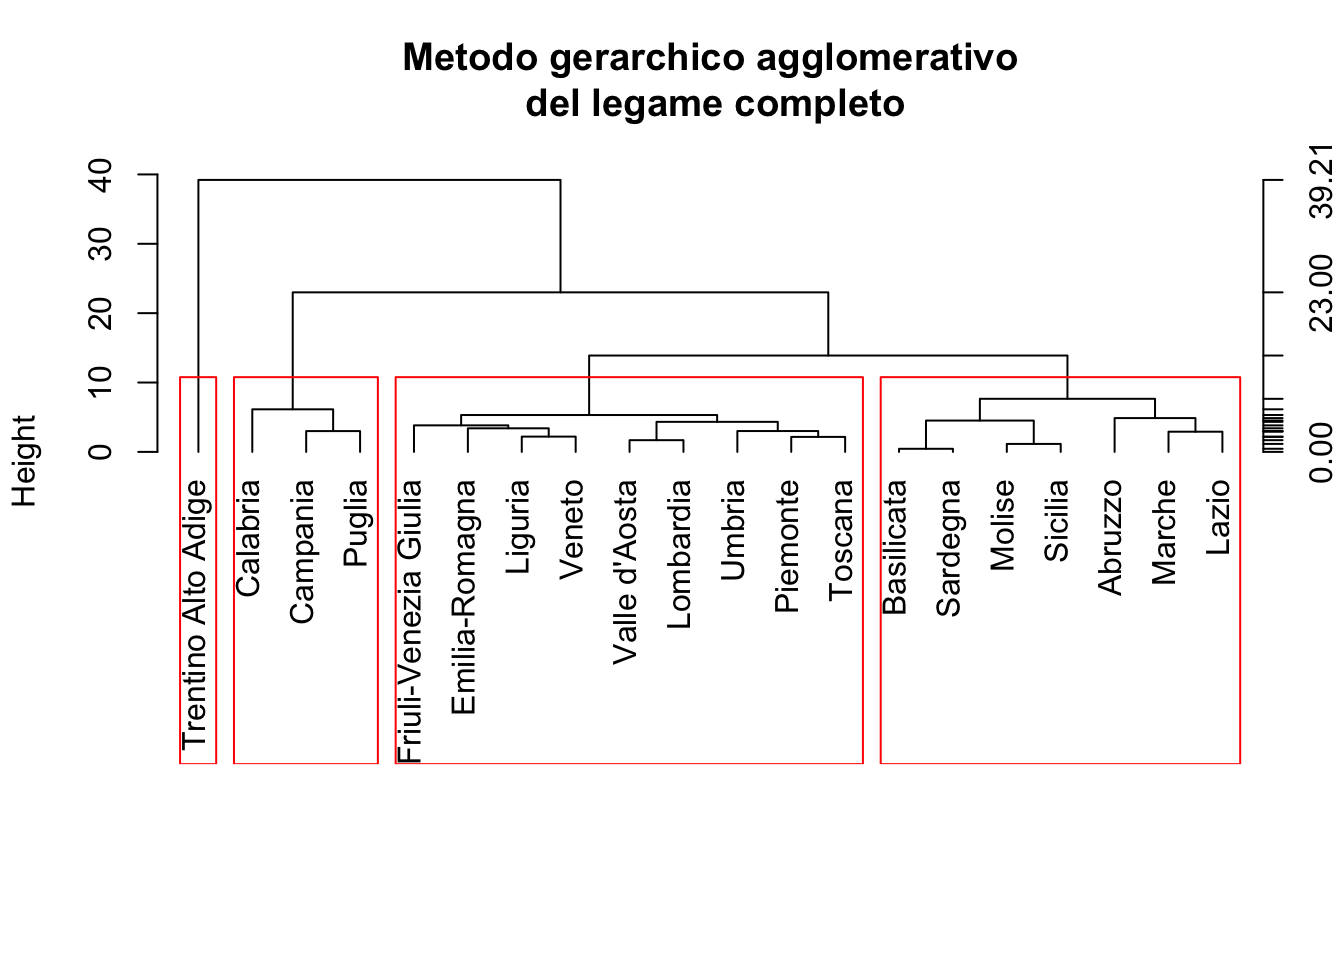
\includegraphics{statistics-project_files/figure-latex/legame-completo-cluster-1} 

}

\caption{Cluster}\label{fig:legame-completo-cluster}
\end{figure}\begin{figure}

{\centering 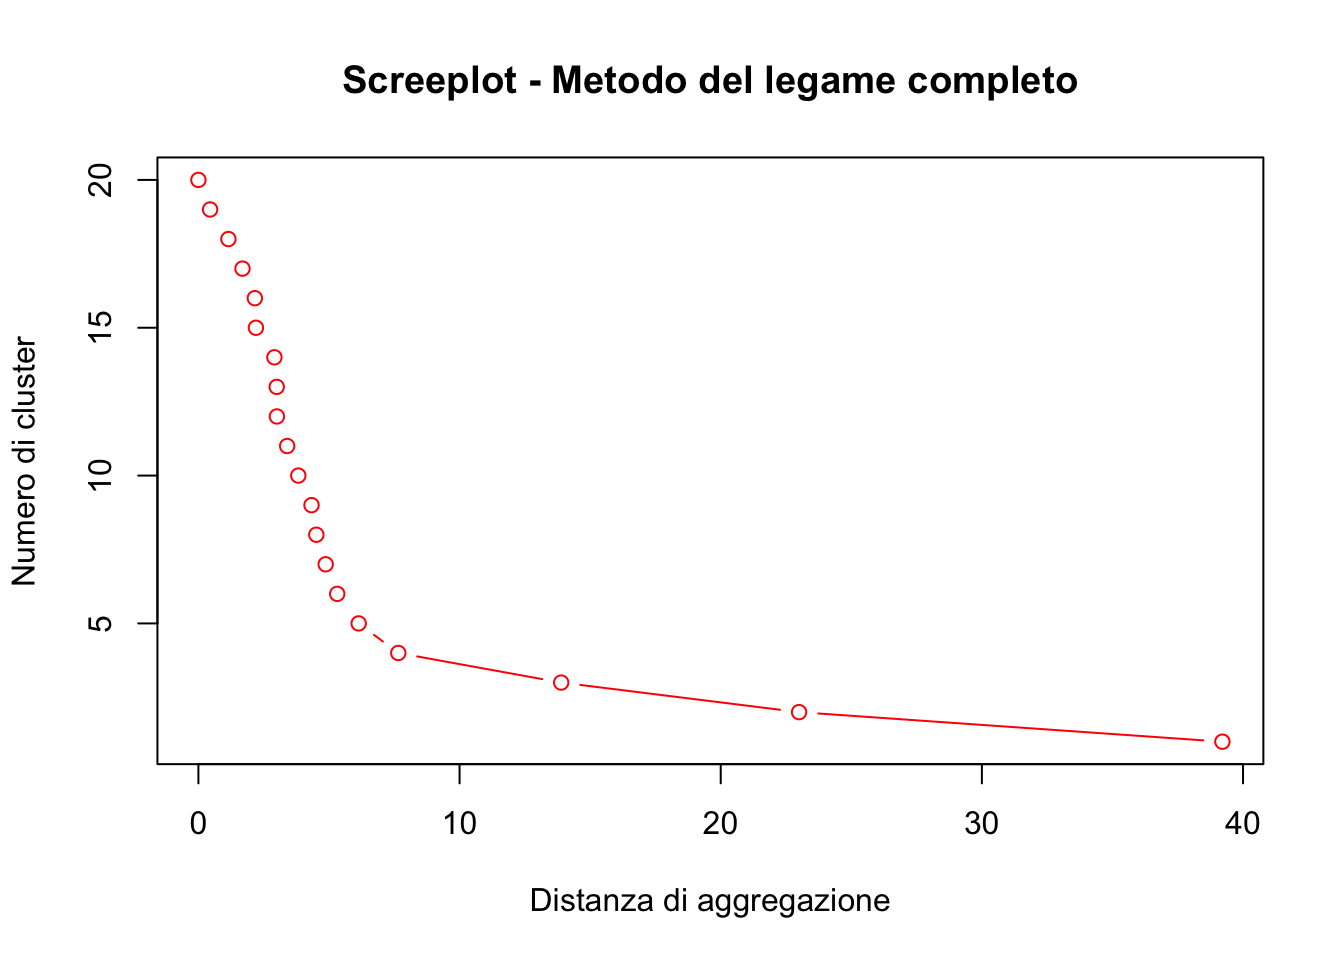
\includegraphics{statistics-project_files/figure-latex/legame-completo-screeplot-1} 

}

\caption{Screeplot}\label{fig:legame-completo-screeplot}
\end{figure}

Nella tabella \ref{tab:legame-completo-misure-omogeneita} sono mostrate
le misure di non omogeneità per il metodo considerato.

\begin{table}

\caption{\label{tab:legame-completo-misure-omogeneita}Misura di non omogeneità}
\centering
\begin{tabular}[t]{l|l|l|l}
\hline
Totale & Within & Between & Between / Totale\\
\hline
1576.9625 & 145.40380952381 & 1431.55869047619 & 0.907795011280351\\
\hline
\end{tabular}
\end{table}

\subsection{Metodo del legame singolo}\label{metodo-del-legame-singolo}

Nel metodo del legame singolo la distanza tra due gruppi è pari alla
minima distanza tra tutte le distanze tra gli individui presi a due a
due in cui uno appartiene a un gruppo e uno all'altro gruppo.

Questo metodo riesce a individuare cluster di qualsiasi forma e mette in
luce valori anomali, di contro può provocare la formazione di catene in
quanto basa l'unione tra i cluster su un solo legame. Di conseguenza ci
può essere un'incapacità di individuare cluster distinti ma non ben
separati.

Il seguente codice è utilizzato per effettuare l'analisi con il metodo
del legame singolo.

\begin{Shaded}
\begin{Highlighting}[]
\NormalTok{hls <-}\StringTok{ }\KeywordTok{hclust}\NormalTok{(d2, }\DataTypeTok{method =} \StringTok{"single"}\NormalTok{)}
\NormalTok{numCluster <-}\StringTok{ }\DecValTok{4}
\NormalTok{misure <-}\StringTok{ }\KeywordTok{calcoloMisure}\NormalTok{(df, hls, numCluster)}
\end{Highlighting}
\end{Shaded}

Nelle figure \ref{fig:legame-singolo-cluster} e
\ref{fig:legame-singolo-screeplot}, sono mostrati il dendrogramma e lo
screeplot. L'analisi dello screeplot suggerisce un numero di cluster
pari a 2, tuttavia si è scelto un numero di cluster pari a 4 per
permettere un confronto con altri metodi.

\begin{figure}

{\centering 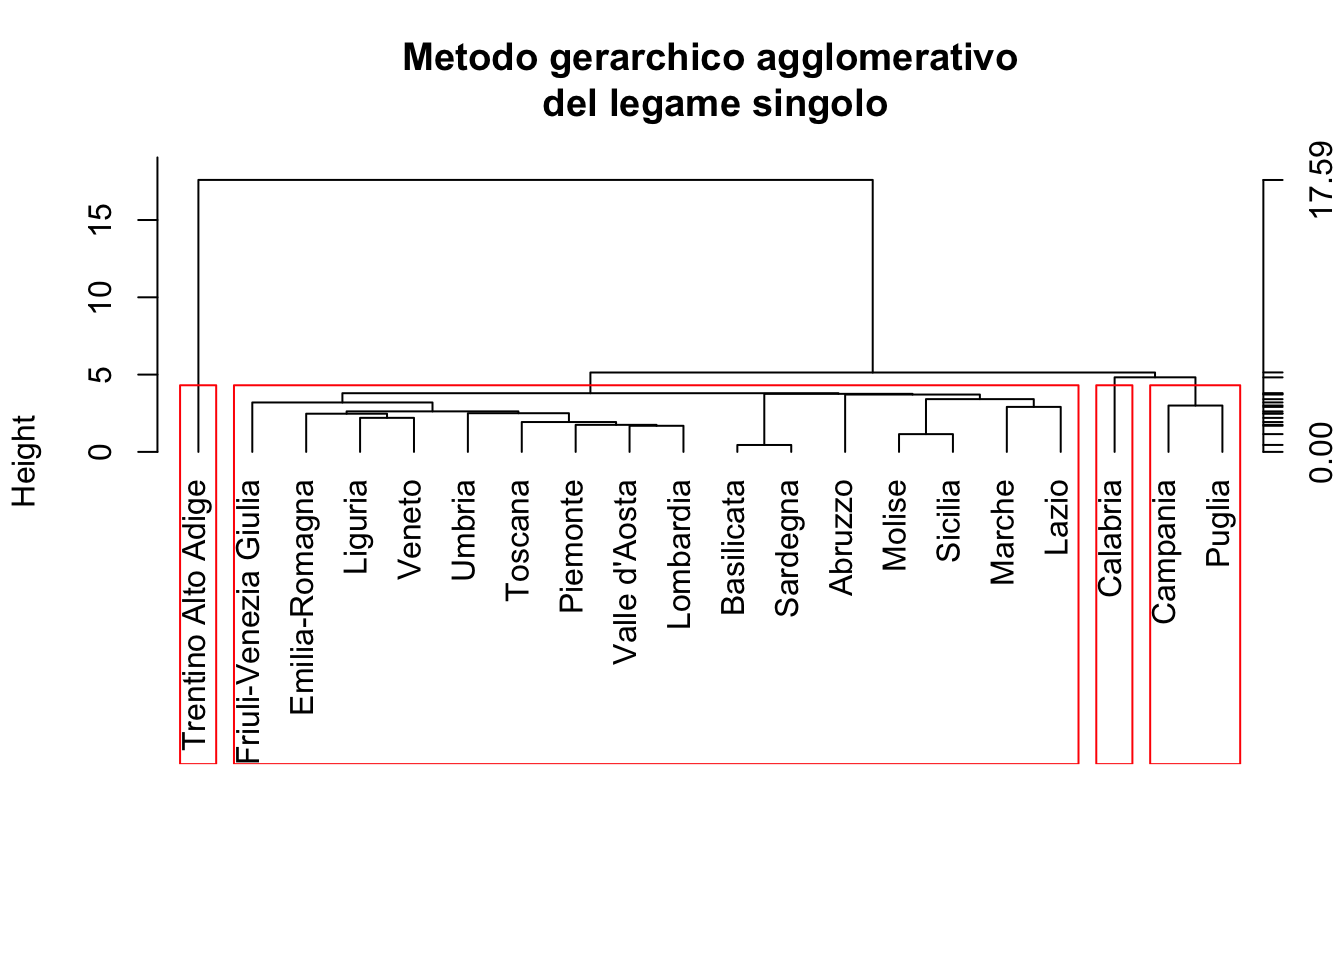
\includegraphics{statistics-project_files/figure-latex/legame-singolo-cluster-1} 

}

\caption{Cluster}\label{fig:legame-singolo-cluster}
\end{figure}

\begin{figure}

{\centering 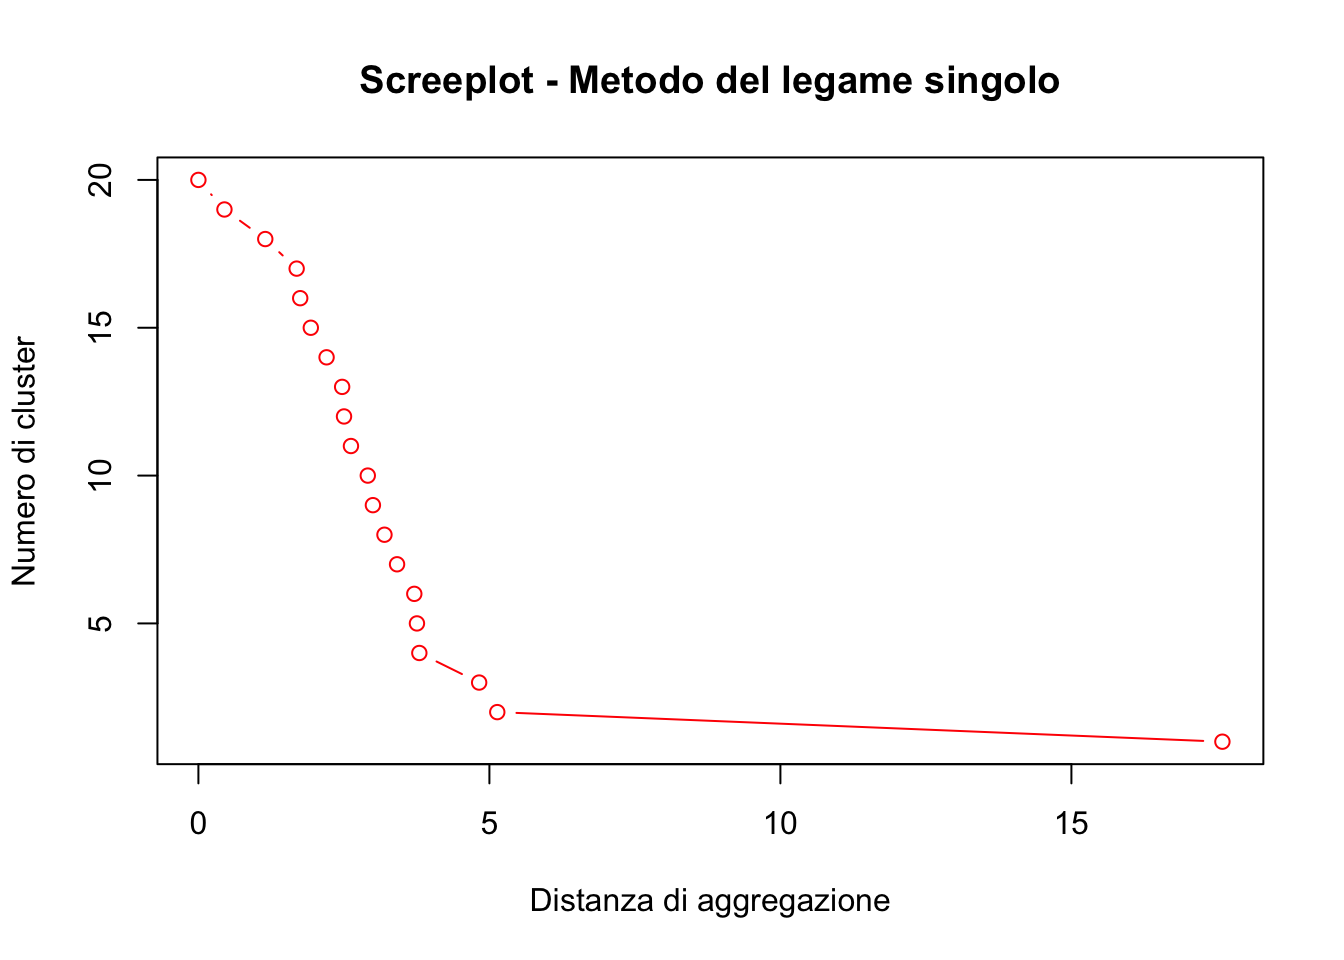
\includegraphics{statistics-project_files/figure-latex/legame-singolo-screeplot-1} 

}

\caption{Screeplot}\label{fig:legame-singolo-screeplot}
\end{figure}

Nella tabella \ref{tab:legame-singolo-misure-omogeneita} sono mostrate
le misure di non omogeneità per il metodo considerato.

\begin{table}

\caption{\label{tab:legame-singolo-misure-omogeneita}Misura di non omogeneità}
\centering
\begin{tabular}[t]{l|l|l|l}
\hline
Totale & Within & Between & Between / Totale\\
\hline
1576.9625 & 423.31875 & 1153.64375 & 0.731560674397774\\
\hline
\end{tabular}
\end{table}

\subsection{Metodo del legame medio}\label{metodo-del-legame-medio}

Nel metodo del legame medio la distanza tra due gruppi è pari alla media
aritmetica tra tutte le distanze tra gli individui presi a due a due in
cui uno appartiene a un gruppo e uno all'altro gruppo.

Va notato che se le dimensioni tra i cluster sono molto differenti la
distanza calcolata sarà molto più vicina a quella del cluster più
numeroso.

Il seguente codice è utilizzato per effettuare l'analisi con il metodo
del legame medio.

\begin{Shaded}
\begin{Highlighting}[]
\NormalTok{hls <-}\StringTok{ }\KeywordTok{hclust}\NormalTok{(d2, }\DataTypeTok{method =} \StringTok{"average"}\NormalTok{)}
\NormalTok{numCluster <-}\StringTok{ }\DecValTok{4}
\NormalTok{misure <-}\StringTok{ }\KeywordTok{calcoloMisure}\NormalTok{(df, hls, numCluster)}
\end{Highlighting}
\end{Shaded}

Nelle figure \ref{fig:legame-medio-cluster} e
\ref{fig:legame-medio-screeplot}, sono mostrati il dendrogramma e lo
screeplot. L'analisi dello screeplot suggerisce un numero di cluster
pari a 2, tuttavia si è scelto un numero di cluster pari a 4 per
permettere un confronto con altri metodi.

\begin{figure}

{\centering 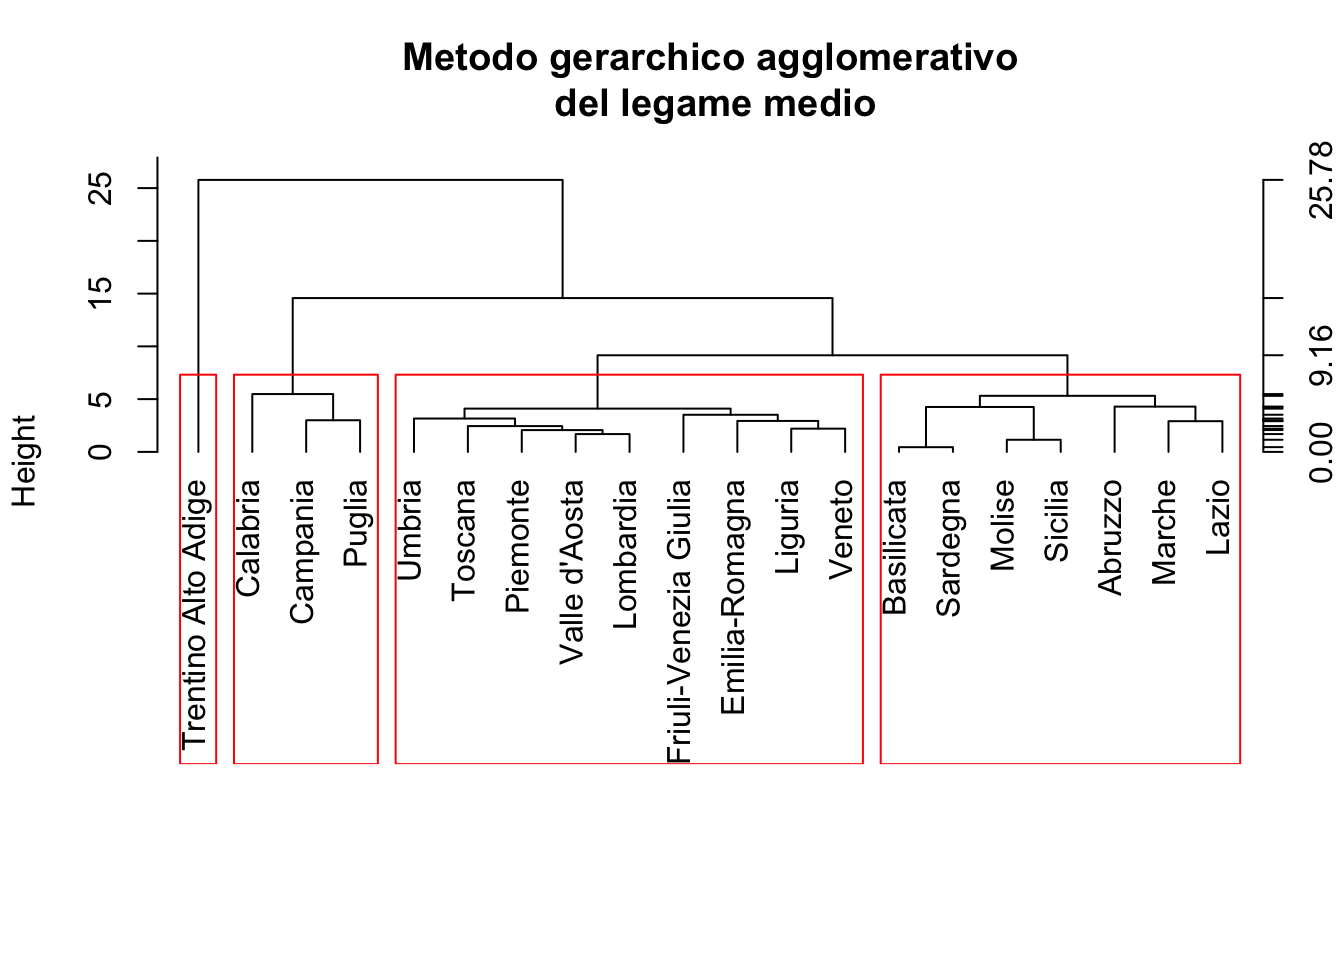
\includegraphics{statistics-project_files/figure-latex/legame-medio-cluster-1} 

}

\caption{Cluster}\label{fig:legame-medio-cluster}
\end{figure}\begin{figure}

{\centering 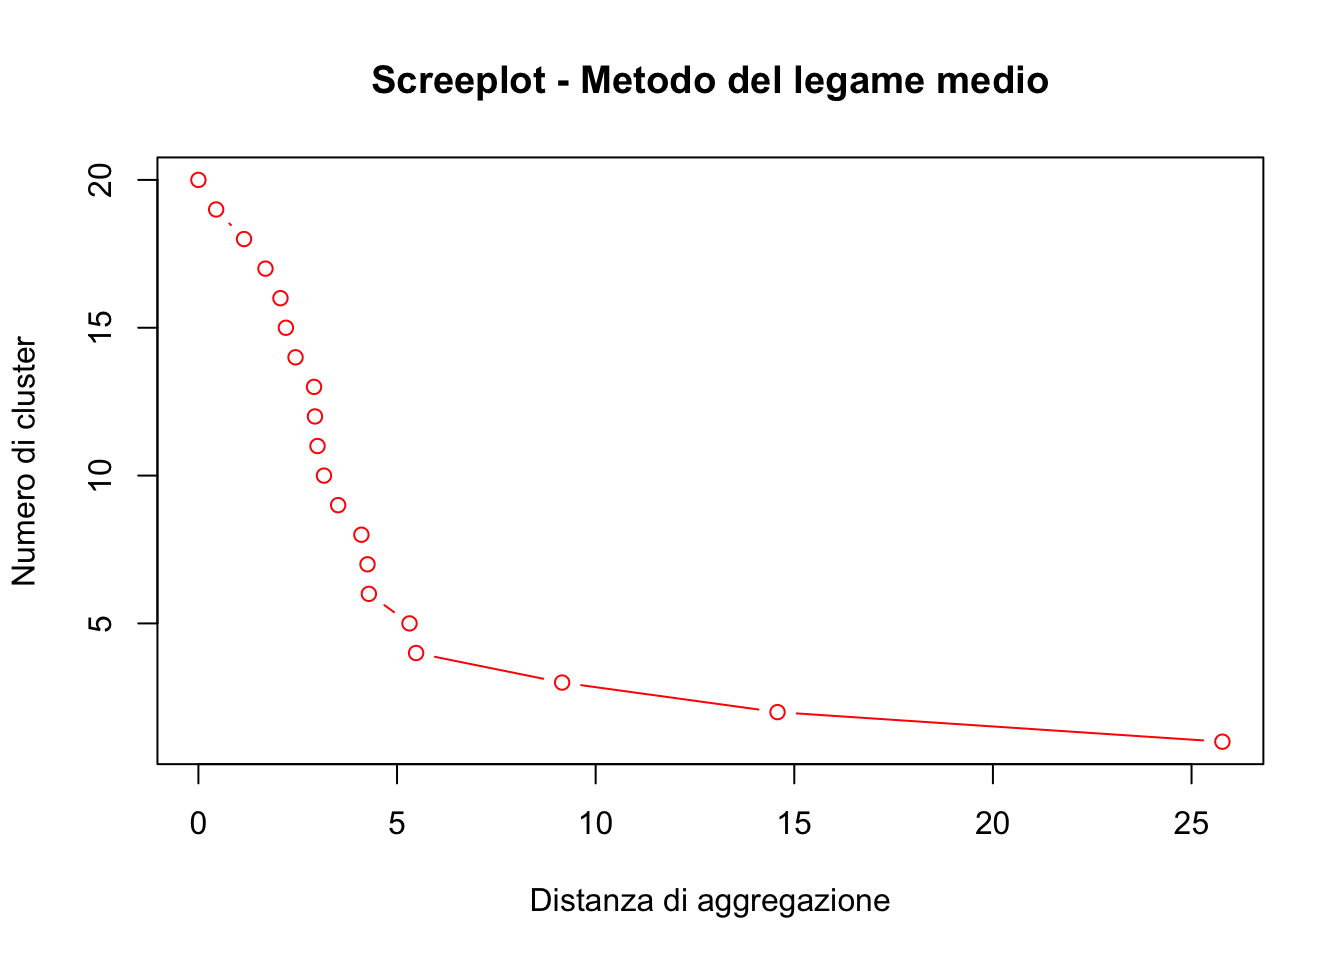
\includegraphics{statistics-project_files/figure-latex/legame-medio-screeplot-1} 

}

\caption{Screeplot}\label{fig:legame-medio-screeplot}
\end{figure}

Nella tabella \ref{tab:legame-medio-misure-omogeneita} sono mostrate le
misure di non omogeneità per il metodo considerato.

\begin{table}

\caption{\label{tab:legame-medio-misure-omogeneita}Misura di non omogeneità}
\centering
\begin{tabular}[t]{l|l|l|l}
\hline
Totale & Within & Between & Between / Totale\\
\hline
1576.9625 & 145.40380952381 & 1431.55869047619 & 0.907795011280351\\
\hline
\end{tabular}
\end{table}

\subsection{Metodo del centroide}\label{metodo-del-centroide}

Nel metodo della mediana la distanza tra due gruppi è pari alla distanza
tra i centroidi, coincidenti con le medie campionarie tra gli individui
dei due gruppi.

Da notare che a differenza dei metodi precedenti il metodo nel centroide
utilizza i quadrati delle distanze euclidee. Utilizzando questo metodo
gruppi grandi potrebbero attrarre gruppi più piccoli, e se le dimensioni
dei cluster sono molto differenti il nuovo centroide sarà più vicino al
cluster più numeroso. Infine le distanze di aggregazione potrebbero
essere non crescenti.

Il seguente codice è utilizzato per effettuare l'analisi con il metodo
del centroide.

\begin{Shaded}
\begin{Highlighting}[]
\NormalTok{hls <-}\StringTok{ }\KeywordTok{hclust}\NormalTok{(square.d2, }\DataTypeTok{method =} \StringTok{"centroid"}\NormalTok{)}
\NormalTok{numCluster <-}\StringTok{ }\DecValTok{4}
\NormalTok{misure <-}\StringTok{ }\KeywordTok{calcoloMisure}\NormalTok{(df, hls, numCluster)}
\end{Highlighting}
\end{Shaded}

Nella figura \ref{fig:legame-centroide-cluster} è mostrato il
dendrogramma con 4 cluster.

\begin{figure}

{\centering 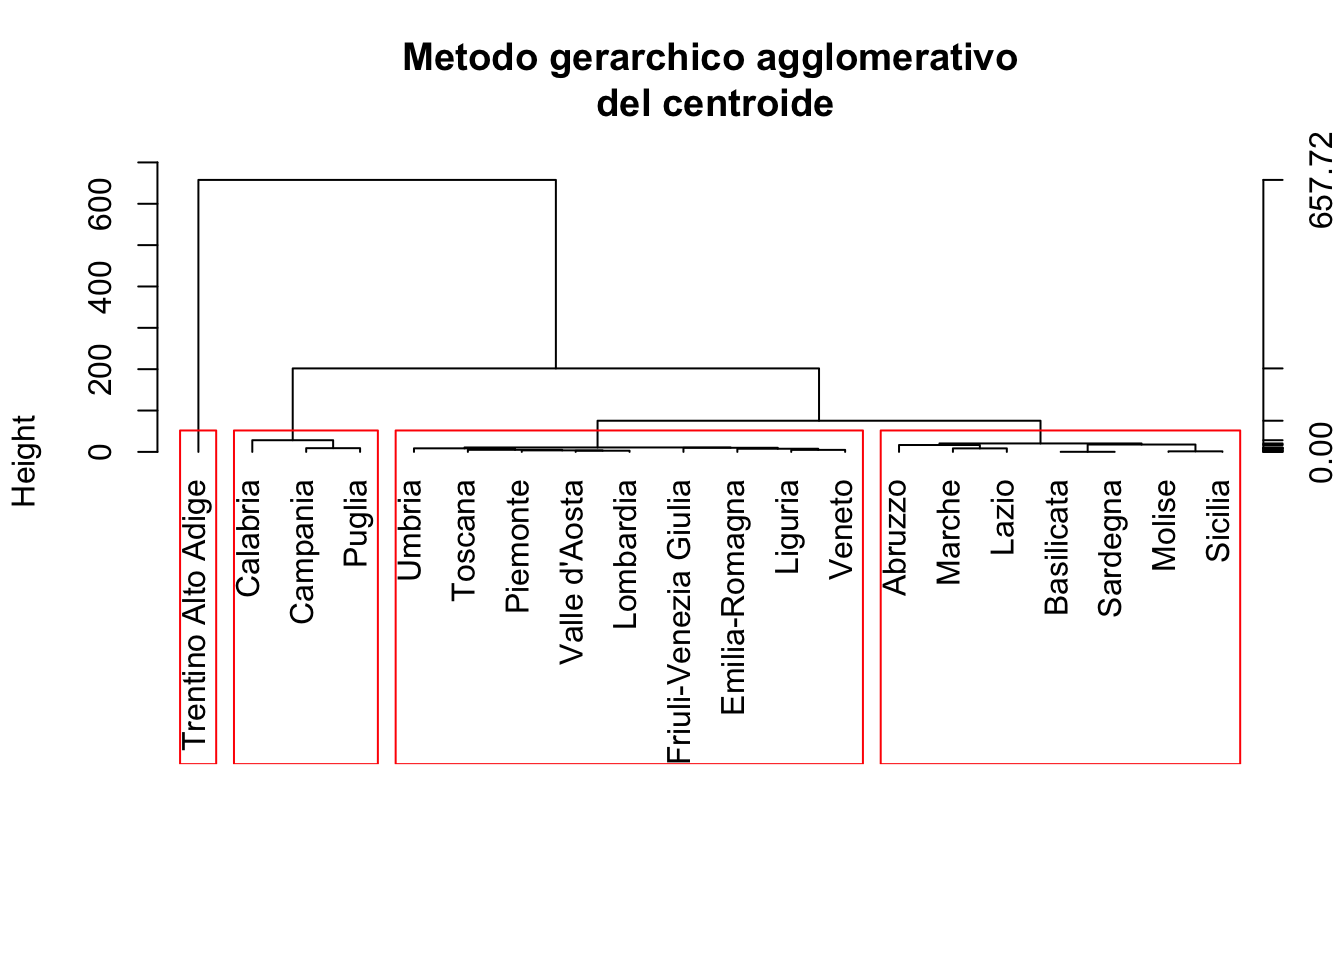
\includegraphics{statistics-project_files/figure-latex/legame-centroide-cluster-1} 

}

\caption{Cluster}\label{fig:legame-centroide-cluster}
\end{figure}

Nella tabella \ref{tab:legame-centroide-misure-omogeneita} sono mostrate
le misure di non omogeneità per il metodo considerato.

\begin{table}

\caption{\label{tab:legame-centroide-misure-omogeneita}Misura di non omogeneità}
\centering
\begin{tabular}[t]{l|l|l|l}
\hline
Totale & Within & Between & Between / Totale\\
\hline
1576.9625 & 145.40380952381 & 1431.55869047619 & 0.907795011280351\\
\hline
\end{tabular}
\end{table}

\subsection{Metodo della mediana}\label{metodo-della-mediana}

Nel metodo della mediana la distanza tra due gruppi è pari alla distanza
tra i centroidi, coincidenti con la media aritmetica dei centroidi dei
due gruppi e di conseguenza è indipendente dalla numerosità dei cluster.

In modo simile al metodo del legame singolo, il metodo nel centroide può
provocare una formazione di una catena.

Il seguente codice è utilizzato per effettuare l'analisi con il metodo
della mediana.

\begin{Shaded}
\begin{Highlighting}[]
\NormalTok{hls <-}\KeywordTok{hclust}\NormalTok{(square.d2, }\DataTypeTok{method =} \StringTok{"median"}\NormalTok{)}
\NormalTok{numCluster <-}\StringTok{ }\DecValTok{4}
\NormalTok{misure <-}\StringTok{ }\KeywordTok{calcoloMisure}\NormalTok{(df, hls, numCluster)}
\end{Highlighting}
\end{Shaded}

Nella figura \ref{fig:legame-mediana-cluster} è mostrato il dendrogramma
con 4 cluster.

\begin{figure}

{\centering 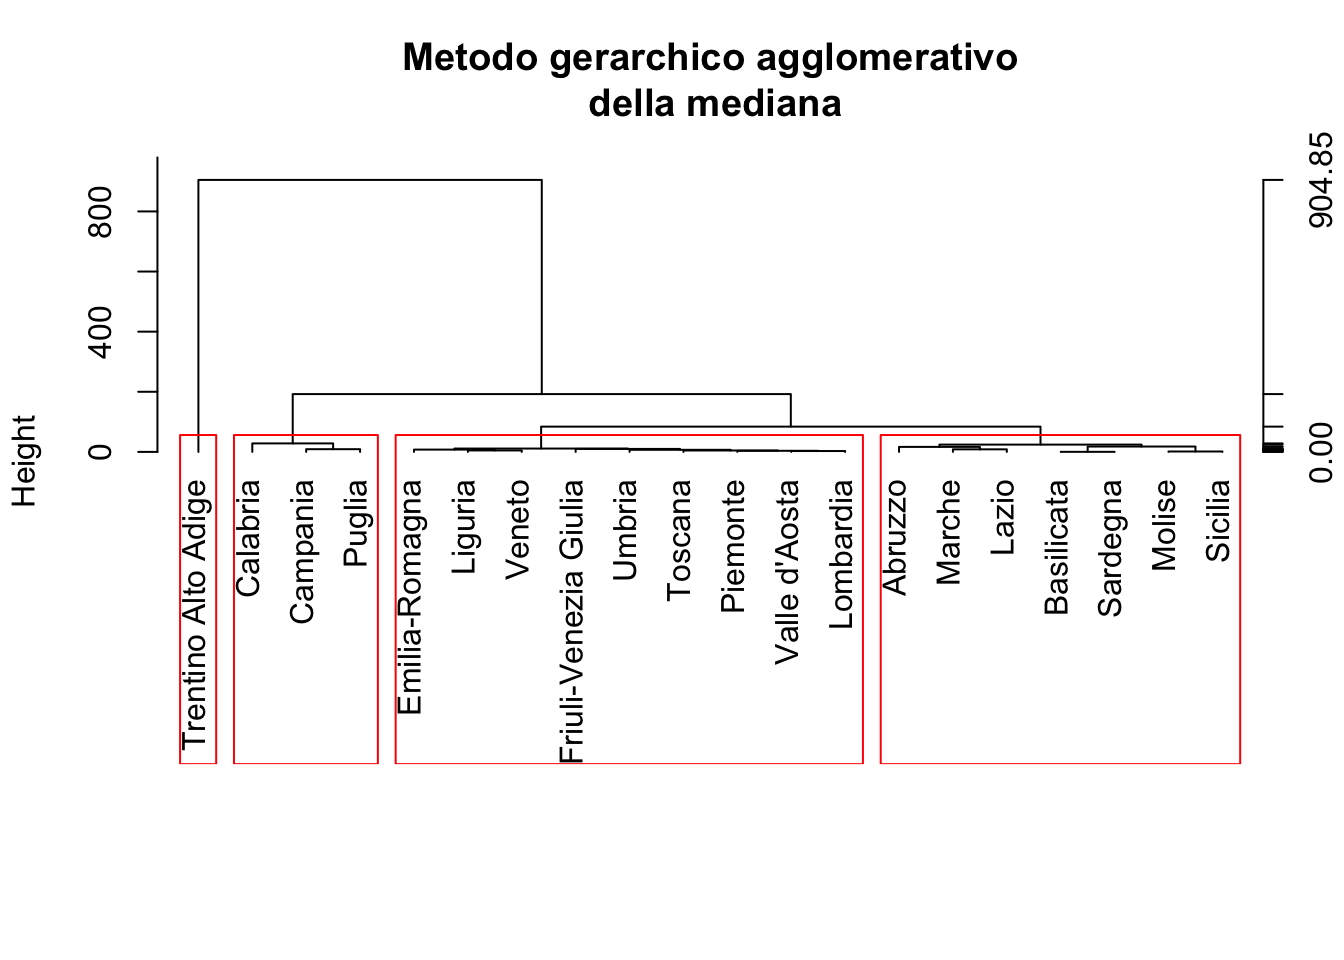
\includegraphics{statistics-project_files/figure-latex/legame-mediana-cluster-1} 

}

\caption{Cluster}\label{fig:legame-mediana-cluster}
\end{figure}

Nella tabella \ref{tab:legame-mediana-misure-omogeneita} sono mostrate
le misure di non omogeneità per il metodo considerato.

\begin{table}

\caption{\label{tab:legame-mediana-misure-omogeneita}Misura di non omogeneità}
\centering
\begin{tabular}[t]{l|l|l|l}
\hline
Totale & Within & Between & Between / Totale\\
\hline
1576.9625 & 145.40380952381 & 1431.55869047619 & 0.907795011280351\\
\hline
\end{tabular}
\end{table}

\subsection{Analisi metodi gerarchici}\label{analisi-metodi-gerarchici}

Nonostante l'analisi degli screen plot abbia suggerito un numero di
cluster pari a due, e stato scelto empiricamente un numero di cluster
pari a quattro. Infatti una suddivisione in due cluster avrebbe avuto in
un cluster l'individuo anomalo ``Trentino Alto-Adige'' e nel restante
gruppo tutte le rimanenti regioni italiane. Con una suddivisione uguale
a quattro si ottengono ottimi risultati, infatti per tutti i metodi
eccetto il metodo del legame singolo, il rapporto tra la misura di non
omogeneità between e quella totale è uguale per tutti i metodi ed ha
valore maggiore di 0.9. Con il metodo nel legame singolo si ottiene
invece un valore inferiore.

Nel seguito vengono analizzati i cluster con il metodo del legame
completo, ottenendo informazioni su alcune misure di sintesi.

Il seguente codice permette di calcolare a quale cluster appartiene ogni
individuo, il numero di individui per cluster e le altezze di
aggregazione. I risultati ottenuti sono mostrati rispettivamente nelle
tabelle: \ref{tab:individui-cluster}, \ref{tab:numero-individui-cluster}
e \ref{tab:altezze}.

\begin{Shaded}
\begin{Highlighting}[]
\NormalTok{individuiInCluster <-}\StringTok{ }\KeywordTok{cutree}\NormalTok{(hls, }\DataTypeTok{k =} \KeywordTok{as.integer}\NormalTok{(numCluster), }\DataTypeTok{h =} \OtherTok{NULL}\NormalTok{)}
\NormalTok{frequenzeAssolute <-}\StringTok{ }\KeywordTok{table}\NormalTok{(individuiInCluster)}
\end{Highlighting}
\end{Shaded}

\begin{table}

\caption{\label{tab:individui-cluster}Individui nei cluster}
\centering
\begin{tabular}[t]{l|r}
\hline
  & Cluster\\
\hline
Piemonte & 1\\
\hline
Valle d'Aosta & 1\\
\hline
Liguria & 1\\
\hline
Lombardia & 1\\
\hline
Veneto & 1\\
\hline
Friuli-Venezia Giulia & 1\\
\hline
Emilia-Romagna & 1\\
\hline
Toscana & 1\\
\hline
Umbria & 1\\
\hline
Trentino Alto Adige & 2\\
\hline
Marche & 3\\
\hline
Lazio & 3\\
\hline
Abruzzo & 3\\
\hline
Molise & 3\\
\hline
Basilicata & 3\\
\hline
Sicilia & 3\\
\hline
Sardegna & 3\\
\hline
Campania & 4\\
\hline
Puglia & 4\\
\hline
Calabria & 4\\
\hline
\end{tabular}
\end{table}

\begin{table}

\caption{\label{tab:numero-individui-cluster}Numero individui nei cluster}
\centering
\begin{tabular}[t]{l|r}
\hline
Cluster & Numero individui\\
\hline
1 & 9\\
\hline
2 & 1\\
\hline
3 & 7\\
\hline
4 & 3\\
\hline
\end{tabular}
\end{table}

\begin{table}

\caption{\label{tab:altezze}Altezze di aggregazione - I numeri negativi indicano gli individui, i numeri positivi i cluster}
\centering
\begin{tabular}[t]{r|r|r}
\hline
Primo individuo/cluster & Secondo individuo/cluster & Altezza\\
\hline
-17 & -20 & 0.200000\\
\hline
-14 & -19 & 1.320000\\
\hline
-2 & -4 & 2.850000\\
\hline
-1 & 3 & 3.652500\\
\hline
-9 & 4 & 4.628125\\
\hline
-3 & -6 & 4.850000\\
\hline
-10 & 5 & 6.924531\\
\hline
-8 & 6 & 7.612500\\
\hline
-11 & -12 & 8.470000\\
\hline
-15 & -16 & 8.990000\\
\hline
-7 & 7 & 9.874883\\
\hline
8 & 11 & 11.103252\\
\hline
-13 & 9 & 16.637500\\
\hline
1 & 2 & 17.800000\\
\hline
13 & 14 & 24.216875\\
\hline
-18 & 10 & 28.217500\\
\hline
12 & 15 & 84.044055\\
\hline
16 & 17 & 192.296307\\
\hline
-5 & 18 & 904.848374\\
\hline
\end{tabular}
\end{table}

Invece il seguente codice permette di calcolare le medie campionarie, le
varianze campionarie e le deviazioni standard campionarie. I risultati
sono mostrati rispettivamente nelle tabelle
\ref{tab:misure-sintesi-medie}, \ref{tab:misure-sintesi-varianze} e
\ref{tab:misure-sintesi-sd}.

\begin{Shaded}
\begin{Highlighting}[]
\NormalTok{hls <-}\StringTok{ }\KeywordTok{hclust}\NormalTok{(d2, }\DataTypeTok{method =} \StringTok{"complete"}\NormalTok{)}
\NormalTok{individuiInCluster <-}\StringTok{ }\KeywordTok{cutree}\NormalTok{(hls, }\DataTypeTok{k =} \KeywordTok{as.integer}\NormalTok{(numCluster), }\DataTypeTok{h =} \OtherTok{NULL}\NormalTok{)}
\NormalTok{indici <-}\StringTok{ }\KeywordTok{list}\NormalTok{(individuiInCluster)}
\NormalTok{medie <-}\StringTok{ }\KeywordTok{aggregate}\NormalTok{(df, indici, mean)}
\NormalTok{varianze <-}\StringTok{ }\KeywordTok{aggregate}\NormalTok{(df, indici, var)}
\NormalTok{deviazioniStandard <-}\StringTok{ }\KeywordTok{aggregate}\NormalTok{(df, indici, sd)}
\end{Highlighting}
\end{Shaded}

Va notato che la varianza e la variazione standard possono essere
calcolate solo se sono presenti almeno due individui. Di conseguenza per
il cluster in cui è presente l'unico individuo ``Trentino Alto-Adige''
tali valori non sono calcolati.

\begin{table}

\caption{\label{tab:misure-sintesi-medie}Medie}
\centering
\begin{tabular}[t]{r|r|r|r|r|r}
\hline
Cluster & Economica & Salute & Famiglia & Amici & Tempo libero\\
\hline
1 & 4.500000 & 18.00000 & 36.90000 & 25.96667 & 15.900000\\
\hline
2 & 10.800000 & 28.70000 & 46.40000 & 35.20000 & 23.800000\\
\hline
3 & 2.471429 & 14.82857 & 31.52857 & 21.82857 & 12.000000\\
\hline
4 & 2.066667 & 11.40000 & 24.83333 & 16.83333 & 9.266667\\
\hline
\end{tabular}
\end{table}

\begin{table}

\caption{\label{tab:misure-sintesi-varianze}Varianze}
\centering
\begin{tabular}[t]{r|r|r|r|r|r}
\hline
Cluster & Economica & Salute & Famiglia & Amici & Tempo libero\\
\hline
1 & 0.8750000 & 1.230000 & 2.682500 & 1.3200000 & 0.5425000\\
\hline
2 & NA & NA & NA & NA & NA\\
\hline
3 & 0.3257143 & 4.979048 & 2.462381 & 2.3890476 & 1.3266667\\
\hline
4 & 0.2233333 & 2.080000 & 8.623333 & 0.7233333 & 0.0033333\\
\hline
\end{tabular}
\end{table}

\begin{table}

\caption{\label{tab:misure-sintesi-sd}Deviazioni standard}
\centering
\begin{tabular}[t]{r|r|r|r|r|r}
\hline
Cluster & Economica & Salute & Famiglia & Amici & Tempo libero\\
\hline
1 & 0.9354143 & 1.109054 & 1.637834 & 1.1489125 & 0.736546\\
\hline
2 & NA & NA & NA & NA & NA\\
\hline
3 & 0.5707138 & 2.231378 & 1.569198 & 1.5456544 & 1.151810\\
\hline
4 & 0.4725816 & 1.442220 & 2.936551 & 0.8504901 & 0.057735\\
\hline
\end{tabular}
\end{table}

\section{Metodo non gerarchico}\label{metodo-non-gerarchico}

Nei paragrafi precedenti abbiamo utilizzato i metodi non gerarchici per
individuare il numero di cluster, in questo paragrafo invece
utilizzeremo il metodo non gerarchico k-means per cercare di ottenere un
migliore raggruppamento degli individui per il numero di cluster scelto.
Questo è possibile in quanto il metodo k-means al contrario dei metodi
gerarchici visti precedentemente consente di riallocare gli individui
nei cluster.

Il metodo funziona nel seguente modo:

\begin{enumerate}
\def\labelenumi{\arabic{enumi}.}
\tightlist
\item
  Fissare il numero \(k\) di cluster, e i punti di riferimento iniziali.
\item
  Associare ogni individuo al cluster più vicino.
\item
  Calcolare il baricentro di ogni cluster.
\item
  Ricalcolare le distanze di ogni individuo da tutti i cluster e
  riallocare gli individui nel cluster più vicino se necessario.
\item
  Ricalcolare il baricentro di ogni cluster.
\item
  Ripetere il procedimento dal punto 4 finché i centroidi non subiscono
  modifiche rispetto all'iterazione precedente.
\end{enumerate}

Va notato che nel metodo k-means si considera la matrice contenente i
quadrati delle distanze euclidee, e che la classificazione finale può
dipendere dalle scelte iniziali.

I punti di riferimento possono essere scelti in modo casuale o
utilizzare i centroidi calcolati con il metodo del centroide, inoltre
può essere fissato a priori il numero massimo di iterazioni. Nel seguito
il numero massimo di iterazioni sarà posto pari a dieci, un numero
maggiore non migliora la classificazione.

Il seguente codice utilizza il metodo k-means scegliendo per dieci volte
i punti di riferimento iniziale in modo casuale.

\begin{Shaded}
\begin{Highlighting}[]
\NormalTok{numCluster <-}\StringTok{ }\DecValTok{4}
\NormalTok{km <-}\StringTok{ }\KeywordTok{kmeans}\NormalTok{(df, }\DataTypeTok{center =}\NormalTok{ numCluster, }\DataTypeTok{iter.max =} \DecValTok{10}\NormalTok{, }\DataTypeTok{nstart =} \DecValTok{10}\NormalTok{)}
\end{Highlighting}
\end{Shaded}

Invece il seguente codice utilizza come centroidi i centroidi calcolati
con il metodo del centroide. Tuttavia con tali punti si ottengono gli
stessi risultati.

\begin{Shaded}
\begin{Highlighting}[]
\NormalTok{hls <-}\StringTok{  }\KeywordTok{hclust}\NormalTok{(square.d2, }\DataTypeTok{method =} \StringTok{"centroid"}\NormalTok{)}
\NormalTok{individuiInCluster <-}\StringTok{ }\KeywordTok{cutree}\NormalTok{(hls, }\DataTypeTok{k =}\NormalTok{ numCluster, }\DataTypeTok{h =} \OtherTok{NULL}\NormalTok{)}
\NormalTok{indici <-}\StringTok{ }\KeywordTok{list}\NormalTok{(individuiInCluster)}
\NormalTok{centroidiIniziali<-}\KeywordTok{aggregate}\NormalTok{(df, indici, mean)[,}\OperatorTok{-}\DecValTok{1}\NormalTok{]}

\NormalTok{km <-}\StringTok{ }\KeywordTok{kmeans}\NormalTok{(df, }\DataTypeTok{center =}\NormalTok{ centroidiIniziali, }\DataTypeTok{iter.max =} \DecValTok{10}\NormalTok{)}
\end{Highlighting}
\end{Shaded}

Nella tabella \ref{tab:kmeans-misure-omogeneita} vengono mostrate le
misure di non omogeneità utilizzando il metodo k-means, mentre nella
tabella \ref{tab:kmeans-cluster} viene mostrato il cluster di
appartenenza di ogni individuo. Come è possibile osservare si ottengono
i medesimi risultati del metodo gerarchico del legame completo.

\begin{table}

\caption{\label{tab:kmeans-misure-omogeneita}Misura di non omogeneità}
\centering
\begin{tabular}[t]{r|r|r|r}
\hline
Totale & Within & Between & Between / Totale\\
\hline
1576.963 & 145.4038 & 1431.559 & 0.907795\\
\hline
\end{tabular}
\end{table}

\begin{table}

\caption{\label{tab:kmeans-cluster}Individui nei cluster}
\centering
\begin{tabular}[t]{l|r}
\hline
  & Cluster\\
\hline
Piemonte & 1\\
\hline
Valle d'Aosta & 1\\
\hline
Liguria & 1\\
\hline
Lombardia & 1\\
\hline
Veneto & 1\\
\hline
Friuli-Venezia Giulia & 1\\
\hline
Emilia-Romagna & 1\\
\hline
Toscana & 1\\
\hline
Umbria & 1\\
\hline
Trentino Alto Adige & 2\\
\hline
Marche & 3\\
\hline
Lazio & 3\\
\hline
Abruzzo & 3\\
\hline
Molise & 3\\
\hline
Basilicata & 3\\
\hline
Sicilia & 3\\
\hline
Sardegna & 3\\
\hline
Campania & 4\\
\hline
Puglia & 4\\
\hline
Calabria & 4\\
\hline
\end{tabular}
\end{table}

Infine vengono mostrati nella tabella \ref{tab:kmeans-centri} i
centroidi dei cluster calcolati.

\begin{table}

\caption{\label{tab:kmeans-centri}Centroidi}
\centering
\begin{tabular}[t]{l|r|r|r|r|r}
\hline
  & Economica & Salute & Famiglia & Amici & Tempo libero\\
\hline
Cluster 1 & 4.500000 & 18.00000 & 36.90000 & 25.96667 & 15.900000\\
\hline
Cluster 2 & 10.800000 & 28.70000 & 46.40000 & 35.20000 & 23.800000\\
\hline
Cluster 3 & 2.471429 & 14.82857 & 31.52857 & 21.82857 & 12.000000\\
\hline
Cluster 4 & 2.066667 & 11.40000 & 24.83333 & 16.83333 & 9.266667\\
\hline
\end{tabular}
\end{table}

\chapter{Distribuzione geometrica}\label{distribuzione-geometrica}

La distribuzione geometrica è una distribuzione di probabilità discreta
il cui nome deriva dal fatto che segue una progressione geometrica, cioè
una successione di numeri tali che è costante il rapporto di un elemento
con il precedente.

Considerato un esperimento consistente nella successione di prove
indipendenti di Bernoulli di parametro \(p \in \{0, 1\}\) e considerato
l'evento

\[E_r = \{ \text{il primo successo si verifica alla prova r-esima}\}\]

allora la probabilità di tale evento è \[P(E_r) = p(1-p)^{r-1}\]

La distribuzione di una variabile aleatoria \(X\) che descrive il numero
di prove per ottenere il primo successo in una successione di prove di
Bernoulli è detta distribuzione geometrica di parametro \(p\)

\[P(X = r) = P(E_r) \quad \text{per} \ r=1,2...\]

e la sua funzione di probabilità per \(0 < p < 1\) è

\[p_X(x) = \begin{cases} p(1-p)^{x-1}, & \mbox{se } x \ge 1 \\ 0, & \mbox{altrimenti} \end{cases}\]

\section{Probabilità teorica e frequenze del
campione}\label{probabilita-teorica-e-frequenze-del-campione}

Il seguente codice permette di calcolare le probabilità che la variabile
aleatoria con distribuzione geometrica di parametro \(p=0.4\) assuma i
valori \(1,...,20\)

\begin{Shaded}
\begin{Highlighting}[]
\NormalTok{p =}\StringTok{ }\FloatTok{0.4}
\NormalTok{minX =}\StringTok{ }\DecValTok{0}
\NormalTok{maxX =}\StringTok{ }\DecValTok{19}
\NormalTok{x =}\StringTok{ }\NormalTok{minX}\OperatorTok{:}\NormalTok{maxX}

\NormalTok{probabilita.x =}\StringTok{ }\NormalTok{x }\OperatorTok{+}\StringTok{ }\DecValTok{1}
\NormalTok{probabilita.y =}\StringTok{ }\KeywordTok{dgeom}\NormalTok{(x, }\DataTypeTok{prob =}\NormalTok{ p)}
\end{Highlighting}
\end{Shaded}

Invece il seguente codice permette di definire un campione di lunghezza
\(200\) estratto da una popolazione descritta da una variabile
geometrica di parametro \(p=0.4\) e di calcolare le frequenze relative
dei valori assunti dal campione.

\begin{Shaded}
\begin{Highlighting}[]
\NormalTok{p =}\StringTok{ }\FloatTok{0.4}
\CommentTok{#campione <- rgeom(100, prob = p) + 1}
\NormalTok{campione <-}\StringTok{ }\KeywordTok{c}\NormalTok{(}\DecValTok{2}\NormalTok{, }\DecValTok{1}\NormalTok{, }\DecValTok{1}\NormalTok{, }\DecValTok{3}\NormalTok{, }\DecValTok{1}\NormalTok{, }\DecValTok{3}\NormalTok{, }\DecValTok{4}\NormalTok{, }\DecValTok{5}\NormalTok{, }\DecValTok{1}\NormalTok{, }\DecValTok{1}\NormalTok{, }\DecValTok{1}\NormalTok{, }\DecValTok{1}\NormalTok{, }\DecValTok{4}\NormalTok{, }\DecValTok{2}\NormalTok{, }\DecValTok{2}\NormalTok{, }\DecValTok{2}\NormalTok{, }\DecValTok{4}\NormalTok{, }\DecValTok{3}\NormalTok{, }\DecValTok{3}\NormalTok{, }\DecValTok{1}\NormalTok{, }
              \DecValTok{1}\NormalTok{, }\DecValTok{1}\NormalTok{, }\DecValTok{2}\NormalTok{, }\DecValTok{2}\NormalTok{, }\DecValTok{1}\NormalTok{, }\DecValTok{1}\NormalTok{, }\DecValTok{1}\NormalTok{, }\DecValTok{2}\NormalTok{, }\DecValTok{3}\NormalTok{, }\DecValTok{6}\NormalTok{, }\DecValTok{3}\NormalTok{, }\DecValTok{1}\NormalTok{, }\DecValTok{6}\NormalTok{, }\DecValTok{1}\NormalTok{, }\DecValTok{1}\NormalTok{, }\DecValTok{2}\NormalTok{, }\DecValTok{1}\NormalTok{, }\DecValTok{4}\NormalTok{, }\DecValTok{1}\NormalTok{, }\DecValTok{1}\NormalTok{, }
              \DecValTok{4}\NormalTok{, }\DecValTok{3}\NormalTok{, }\DecValTok{2}\NormalTok{, }\DecValTok{1}\NormalTok{, }\DecValTok{4}\NormalTok{, }\DecValTok{6}\NormalTok{, }\DecValTok{7}\NormalTok{, }\DecValTok{2}\NormalTok{, }\DecValTok{1}\NormalTok{, }\DecValTok{1}\NormalTok{, }\DecValTok{3}\NormalTok{, }\DecValTok{1}\NormalTok{, }\DecValTok{1}\NormalTok{, }\DecValTok{4}\NormalTok{, }\DecValTok{1}\NormalTok{, }\DecValTok{1}\NormalTok{, }\DecValTok{4}\NormalTok{, }\DecValTok{1}\NormalTok{, }\DecValTok{4}\NormalTok{, }\DecValTok{1}\NormalTok{, }
              \DecValTok{2}\NormalTok{, }\DecValTok{1}\NormalTok{, }\DecValTok{1}\NormalTok{, }\DecValTok{1}\NormalTok{, }\DecValTok{4}\NormalTok{, }\DecValTok{2}\NormalTok{, }\DecValTok{1}\NormalTok{, }\DecValTok{2}\NormalTok{, }\DecValTok{3}\NormalTok{, }\DecValTok{2}\NormalTok{, }\DecValTok{2}\NormalTok{, }\DecValTok{1}\NormalTok{, }\DecValTok{2}\NormalTok{, }\DecValTok{1}\NormalTok{, }\DecValTok{2}\NormalTok{, }\DecValTok{1}\NormalTok{, }\DecValTok{2}\NormalTok{, }\DecValTok{2}\NormalTok{, }\DecValTok{6}\NormalTok{, }\DecValTok{5}\NormalTok{, }
              \DecValTok{6}\NormalTok{, }\DecValTok{2}\NormalTok{, }\DecValTok{6}\NormalTok{, }\DecValTok{2}\NormalTok{, }\DecValTok{3}\NormalTok{, }\DecValTok{2}\NormalTok{, }\DecValTok{2}\NormalTok{, }\DecValTok{2}\NormalTok{, }\DecValTok{4}\NormalTok{, }\DecValTok{1}\NormalTok{, }\DecValTok{1}\NormalTok{, }\DecValTok{1}\NormalTok{, }\DecValTok{1}\NormalTok{, }\DecValTok{2}\NormalTok{, }\DecValTok{3}\NormalTok{, }\DecValTok{9}\NormalTok{, }\DecValTok{3}\NormalTok{, }\DecValTok{1}\NormalTok{, }\DecValTok{2}\NormalTok{, }\DecValTok{1}\NormalTok{)}
\NormalTok{frequenzeRelative <-}\StringTok{ }\KeywordTok{table}\NormalTok{(campione) }\OperatorTok{/}\StringTok{ }\KeywordTok{length}\NormalTok{(campione)}
\end{Highlighting}
\end{Shaded}

In figura \ref{fig:probabilita-frequenze-geometrica} sono mostrate le
probabilità della distribuzione geometrica e le frequenze del campione
calcolate dal codice precedente. Come è possibile notare, per campioni
numerosi, le frequenze relative tendono alla probabilità teoriche.

\begin{figure}

{\centering 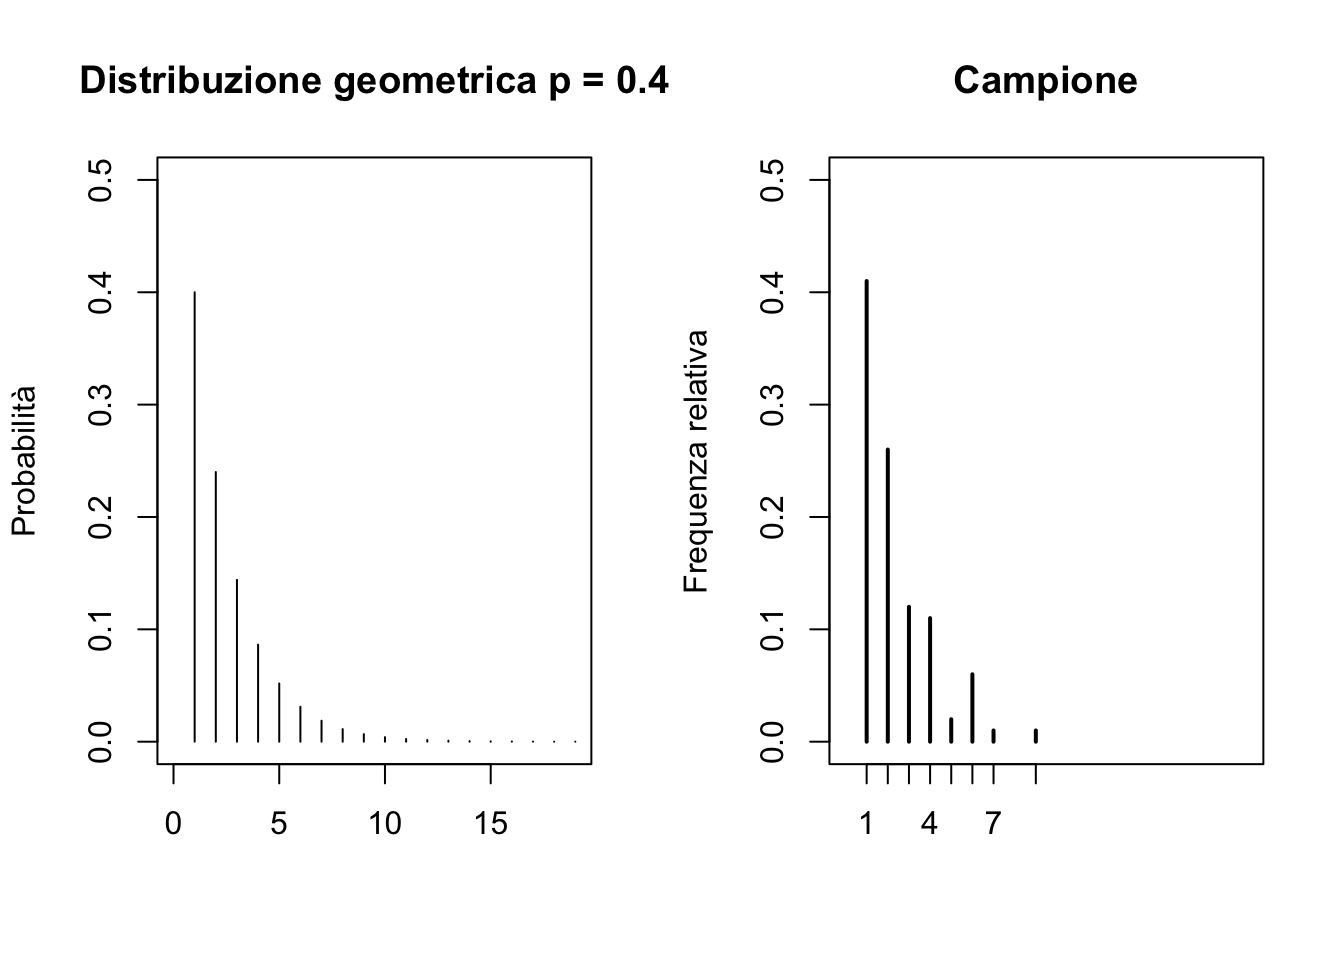
\includegraphics{statistics-project_files/figure-latex/probabilita-frequenze-geometrica-1} 

}

\caption{Probabilità teoriche e frequenze relative del campione}\label{fig:probabilita-frequenze-geometrica}
\end{figure}

\section{Funzione di distribuzione}\label{funzione-di-distribuzione}

Calcolata la somma delle prime \(k\) probabilità

\[\sum_{r=1}^{k}p_X(r) = \sum_{r=1}^{k}p(1-p)^{r-1} = p \sum_{s = 0}^{k - 1} (1 - p)^s = p \frac{1-(1-p)^k}{1-(1-p)} = 1 - (1 - p)^k\]
La funzione di distribuzione per una distribuzione geometrica di
parametro \(p\) è definita con il valore

\[F_X(x) = P(X \le x) =  \begin{cases} 0, & \mbox{se } x < 1 \\ 1 - (1 - p)^k, & \mbox{se } k \le x < k + 1 \end{cases}\]

Il seguente codice consente di calcolare i valori che assume la funzione
di distribuzione di frequenza tra 1 e 20. Il relativo grafico è mostrato
in figura \ref{fig:geometrica-distribuzione}

\begin{Shaded}
\begin{Highlighting}[]
\NormalTok{distribuzione <-}\StringTok{ }\KeywordTok{pgeom}\NormalTok{(x, }\DataTypeTok{prob =}\NormalTok{ p, }\DataTypeTok{lower.tail =} \OtherTok{TRUE}\NormalTok{)}
\end{Highlighting}
\end{Shaded}

\begin{figure}

{\centering 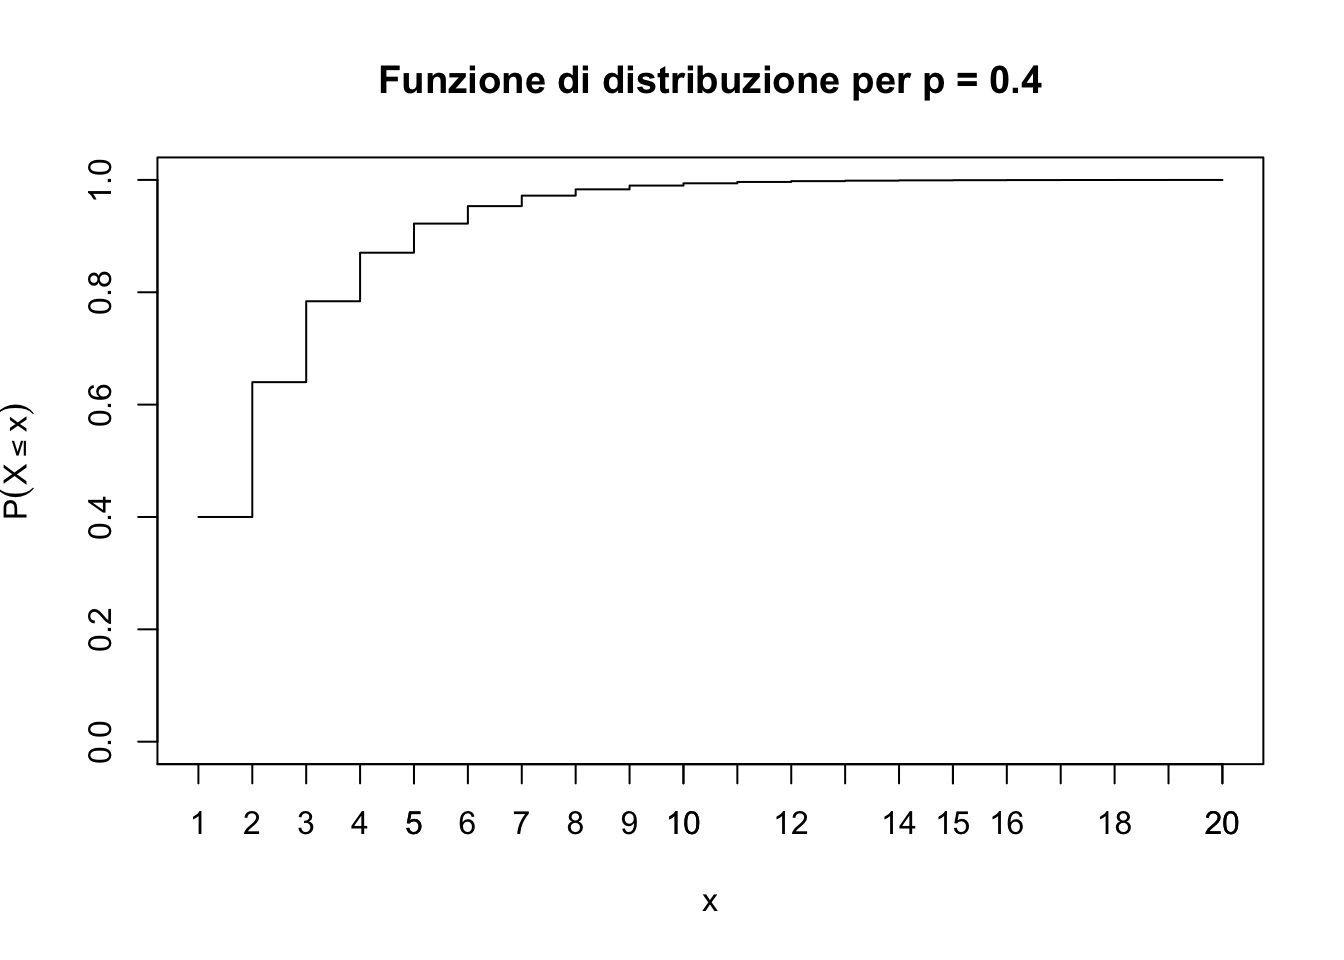
\includegraphics{statistics-project_files/figure-latex/geometrica-distribuzione-1} 

}

\caption{Funzione di distribuzione}\label{fig:geometrica-distribuzione}
\end{figure}

\section{Quantili}\label{quantili-1}

Il percentile \(z * 100\)-esimo è il più piccolo \(k\) tale che
\[P(X \le x) = 1 - (1 - p)^k > z\]

Il valore di \(k\) può essere calcolato algebricamente con nel seguente
modo
\[1 - (1 - p)^k > z \Leftrightarrow (1 - p)^k < 1 - z \Leftrightarrow k \ge \frac{log{(1 - z)}}{log(1 - p)}\]

\textbf{Mediana}

Ad esempio se vogliamo calcolare la mediana, cioè il percentile
\(0.5 * 100\)-esimo allora bisogna scegliere il più piccolo \(k\) tale
che \(k \ge \frac{log(1-0.5)}{log(1-0.4) }\)

Il seguente codice effettua il calcolo

\begin{Shaded}
\begin{Highlighting}[]
\NormalTok{mediana <-}\StringTok{ }\KeywordTok{ceiling}\NormalTok{(}\KeywordTok{log}\NormalTok{(}\DecValTok{1}\OperatorTok{-}\FloatTok{0.5}\NormalTok{) }\OperatorTok{/}\StringTok{ }\KeywordTok{log}\NormalTok{(}\DecValTok{1}\OperatorTok{-}\NormalTok{p))}
\end{Highlighting}
\end{Shaded}

Il risultato ottenuto è 2.

\textbf{Quartili}

Invece il seguente codice calcola i quartili utilizzando la funzione
\emph{qgeom}. I risultati ottenuti sono mostrati in tabella
\ref{tab:geometrica-quartili}

\begin{Shaded}
\begin{Highlighting}[]
\NormalTok{quartili <-}\StringTok{ }\KeywordTok{qgeom}\NormalTok{(}\KeywordTok{c}\NormalTok{(}\FloatTok{0.25}\NormalTok{, }\FloatTok{0.5}\NormalTok{, }\FloatTok{0.75}\NormalTok{, }\DecValTok{1}\NormalTok{), }\DataTypeTok{prob =}\NormalTok{ p, }\DataTypeTok{lower.tail =} \OtherTok{TRUE}\NormalTok{) }\OperatorTok{+}\StringTok{ }\DecValTok{1}
\end{Highlighting}
\end{Shaded}

\begin{table}

\caption{\label{tab:geometrica-quartili}Quartili}
\centering
\begin{tabular}[t]{r|r|r|r}
\hline
Primo quartile & Secondo quartile & Terzo quartile & Quarto quartile\\
\hline
1 & 2 & 3 & Inf\\
\hline
\end{tabular}
\end{table}

Come è possibile notare il valore della mediana (secondo quartile)
assume valore pari a 2 con entrambi i metodi.

\section{Valore atteso e varianza}\label{valore-atteso-e-varianza}

Per una variabile aleatoria descritta da una distribuzione geometrica di
parametro \(p\) il valore atteso è \[E(X) = \frac{1}{p}\] mentre la
varianza è

\[Var(X) = \frac{1 - p}{p^2}\]

Il seguente codice calcola il valore atteso e la varianza della
variabile geometrica di parametro p, e la media campionaria e la
varianza campionaria del campione simulato. I risultati ottenuti sono
mostrati in tabella \ref{tab:geometrica-statistiche}

\begin{Shaded}
\begin{Highlighting}[]
\NormalTok{valore.atteso <-}\StringTok{ }\DecValTok{1} \OperatorTok{/}\StringTok{ }\NormalTok{p}
\NormalTok{media.campionaria <-}\StringTok{ }\KeywordTok{mean}\NormalTok{(campione)}

\NormalTok{varianza <-}\StringTok{ }\NormalTok{(}\DecValTok{1} \OperatorTok{-}\StringTok{ }\NormalTok{p) }\OperatorTok{/}\StringTok{ }\NormalTok{p}\OperatorTok{^}\DecValTok{2}
\NormalTok{varianzaCampionaria <-}\StringTok{ }\KeywordTok{var}\NormalTok{(campione)}
\end{Highlighting}
\end{Shaded}

\begin{table}

\caption{\label{tab:geometrica-statistiche}Statistiche}
\centering
\begin{tabular}[t]{r|r|r|r}
\hline
Media & Media campionaria & Varianza & Varianza campionaria\\
\hline
2.5 & 2.35 & 3.75 & 2.75505\\
\hline
\end{tabular}
\end{table}

\section{Assenza di memoria}\label{assenza-di-memoria}

Una variabile aleatoria \(X\) con distribuzione geometrica gode della
proprietà di assenza di memoria
\[P(X > r + n \ | \ X > r) = P(X > n) \quad \text{con r e n interi non negativi}\]

Ciò significa che pur sapendo che nelle prime \(r\) prove non c'è stato
un successo, la probabilità che che non si verifica un successo fino
alla prova \(r + n\) dipende soltanto dalle \(n\) prove da effettuare e
non dalle \(r\) prove già effettuate.

\chapter{Stima puntuale}\label{stima-puntuale}

Un problema dell'inferenza statistica è lo studio di una popolazione
descritta da una variabile aleatoria osservabile e avente una funzione
di distribuzione nota eccetto per uno o più parametri non noti

Uno stimatore è una funzione misurabile e osservabile che associa a un
campione un valore per il parametro da stimare. Il valore assunto dallo
stimatore è detto stima.

Nel seguito verranno mostrati due metodi di stima dei parametri, il
metodo dei momenti e il metodo della massima verosimiglianza.

\section{Metodo dei momenti}\label{metodo-dei-momenti}

Si definisce momento campionari r-esimo di un campione \((x_1,...,x_n)\)
il valore \[M_r(x_1,...,x_n) = \frac{1}{n}\sum_{i=1}^nx_i^r\]

mentre si definisce momento campionario di una variabile aleatoria il
valore \[M_r(X) = E(X^r)\]

Il metodo dei momenti consiste nell'uguagliare i momenti campionari e i
momenti non osservabili della variabile aleatoria caratterizzante la
popolazione. Le soluzioni risultanti sono gli stimatori dei parametri
non noti.

Formalmente, se si desidera stimare \(k\) parametri
\(\theta_1,...,\theta_k\) non noti di una distribuzione di probabilità
\(f_X(x;\theta_1,...,\theta_k)\) della variabile aleatoria \(X\) si
calcolano i primi \(k\) momenti della variabile aleatoria \(X\)
\[\mu_i = E[X^i] = g_i(\theta_1,...,\theta_k) \quad \text{per} \ i = 1,...,k\]
e dato un campione estratto \((x_1,...,x_n)\) si calcolano i primi \(k\)
momenti del campione\\
\[\hat{\mu_i} = M_r(x_1,...,x_n) \quad \text{per} \ i = 1,...,k \]

Lo stimatore del metodo dei momenti per \(\theta_1,...,\theta_k\)
denotato da \(\hat\theta_1,...,\hat\theta_k\) se esiste è la soluzione
del sistema di equazioni
\[\hat{\mu_i} = g_i(\hat\theta_1,...,\hat\theta_k)  \quad \text{per} \ i = 1,...,k \]
Essendo gli stimatori dipendenti dal campione ne consegue che al variare
dei campioni si potrebbero ottenere stimatori diversi.

\subsection{Stima per la popolazione
geometrica}\label{stima-per-la-popolazione-geometrica}

In questo paragrafo verrà stimato il parametro \(p\) di una
distribuzione geometrica con il metodo dei momenti.

Il momento campionario primo della variabile geometrica è
\[\mu_1 = E[X^1] = \frac{1}{p}\] mentre il momento campionario primo del
campione è

\[\hat\mu_1 = \frac{1}{n}\sum_{i=1}^nx_i = \overline{x}\]

Ne consegue che la media campionaria \(\overline{x}\) è uno stimatore
per \(\frac{1}{p}\)

Il seguente codice definisce un campione proveniente da una
distribuzione geometrica di parametro \(p\) non noto e stima il
parametro \(p\) con il metodo dei momenti.

\begin{Shaded}
\begin{Highlighting}[]
\NormalTok{campione <-}\StringTok{ }\KeywordTok{c}\NormalTok{(}\DecValTok{2}\NormalTok{, }\DecValTok{1}\NormalTok{, }\DecValTok{1}\NormalTok{, }\DecValTok{3}\NormalTok{, }\DecValTok{1}\NormalTok{, }\DecValTok{3}\NormalTok{, }\DecValTok{4}\NormalTok{, }\DecValTok{5}\NormalTok{, }\DecValTok{1}\NormalTok{, }\DecValTok{1}\NormalTok{, }\DecValTok{1}\NormalTok{, }\DecValTok{1}\NormalTok{, }\DecValTok{4}\NormalTok{, }\DecValTok{2}\NormalTok{, }\DecValTok{2}\NormalTok{, }\DecValTok{2}\NormalTok{, }\DecValTok{4}\NormalTok{, }\DecValTok{3}\NormalTok{, }\DecValTok{3}\NormalTok{, }\DecValTok{1}\NormalTok{, }
         \DecValTok{1}\NormalTok{, }\DecValTok{1}\NormalTok{, }\DecValTok{2}\NormalTok{, }\DecValTok{2}\NormalTok{, }\DecValTok{1}\NormalTok{, }\DecValTok{1}\NormalTok{, }\DecValTok{1}\NormalTok{, }\DecValTok{2}\NormalTok{, }\DecValTok{3}\NormalTok{, }\DecValTok{6}\NormalTok{, }\DecValTok{3}\NormalTok{, }\DecValTok{1}\NormalTok{, }\DecValTok{6}\NormalTok{, }\DecValTok{1}\NormalTok{, }\DecValTok{1}\NormalTok{, }\DecValTok{2}\NormalTok{, }\DecValTok{1}\NormalTok{, }\DecValTok{4}\NormalTok{, }\DecValTok{1}\NormalTok{, }\DecValTok{1}\NormalTok{, }
         \DecValTok{4}\NormalTok{, }\DecValTok{3}\NormalTok{, }\DecValTok{2}\NormalTok{, }\DecValTok{1}\NormalTok{, }\DecValTok{4}\NormalTok{, }\DecValTok{6}\NormalTok{, }\DecValTok{7}\NormalTok{, }\DecValTok{2}\NormalTok{, }\DecValTok{1}\NormalTok{, }\DecValTok{1}\NormalTok{, }\DecValTok{3}\NormalTok{, }\DecValTok{1}\NormalTok{, }\DecValTok{1}\NormalTok{, }\DecValTok{4}\NormalTok{, }\DecValTok{1}\NormalTok{, }\DecValTok{1}\NormalTok{, }\DecValTok{4}\NormalTok{, }\DecValTok{1}\NormalTok{, }\DecValTok{4}\NormalTok{, }\DecValTok{1}\NormalTok{, }
         \DecValTok{2}\NormalTok{, }\DecValTok{1}\NormalTok{, }\DecValTok{1}\NormalTok{, }\DecValTok{1}\NormalTok{, }\DecValTok{4}\NormalTok{, }\DecValTok{2}\NormalTok{, }\DecValTok{1}\NormalTok{, }\DecValTok{2}\NormalTok{, }\DecValTok{3}\NormalTok{, }\DecValTok{2}\NormalTok{, }\DecValTok{2}\NormalTok{, }\DecValTok{1}\NormalTok{, }\DecValTok{2}\NormalTok{, }\DecValTok{1}\NormalTok{, }\DecValTok{2}\NormalTok{, }\DecValTok{1}\NormalTok{, }\DecValTok{2}\NormalTok{, }\DecValTok{2}\NormalTok{, }\DecValTok{6}\NormalTok{, }\DecValTok{5}\NormalTok{, }
         \DecValTok{6}\NormalTok{, }\DecValTok{2}\NormalTok{, }\DecValTok{6}\NormalTok{, }\DecValTok{2}\NormalTok{, }\DecValTok{3}\NormalTok{, }\DecValTok{2}\NormalTok{, }\DecValTok{2}\NormalTok{, }\DecValTok{2}\NormalTok{, }\DecValTok{4}\NormalTok{, }\DecValTok{1}\NormalTok{, }\DecValTok{1}\NormalTok{, }\DecValTok{1}\NormalTok{, }\DecValTok{1}\NormalTok{, }\DecValTok{2}\NormalTok{, }\DecValTok{3}\NormalTok{, }\DecValTok{9}\NormalTok{, }\DecValTok{3}\NormalTok{, }\DecValTok{1}\NormalTok{, }\DecValTok{2}\NormalTok{, }\DecValTok{1}\NormalTok{)}

\NormalTok{stima.p <-}\StringTok{ }\DecValTok{1} \OperatorTok{/}\StringTok{ }\KeywordTok{mean}\NormalTok{(campione) }
\end{Highlighting}
\end{Shaded}

Il valore calcolato pari a 0.4255319 è il valore stimato del parametro
p.

\section{Metodo della massima
verosimiglianza}\label{metodo-della-massima-verosimiglianza}

Se \(X_1,..., X_k\) è un campione casuale si definisce funzione di
verosimiglianza
\[L(\theta_1,...,\theta_k) = L(\theta_1,...,\theta_k; x_1,...,x_k) = f(x_1;\theta_1,...,\theta_k) \cdots f(x_n;\theta_1,...,\theta_k)\]
del campione osservato \((x_1,...,x_k)\) la funzione di probabilità
congiunta se la popolazione è discreta o la funzione di densità di
probabilità congiunta se la popolazione è assolutamente continua, del
campione casuale \(X_1,..., X_k\).

Il metodo della massima verosimiglianza consiste nel massimizzare la
funzione di verosimiglianza rispetto ai parametri non noti e quindi
trovare i parametri della funzione di probabilità o di densità di
probabilità per la quale sia più verosimile la provenienza del campione.

I valori \(\hat\theta_1,...,\hat\theta_k\) che massimizzano la funzione
di verosimiglianza sono detti stime di massima verosimiglianza dei
parametri non noti \(\theta_1,...,\theta_k\). Essendo le stime
dipendenti dal campione ne consegue che al variare dei campioni si
possono ottenere stimatori diversi dei parametri non noti.

\subsection{Stima per la popolazione
geometrica}\label{stima-per-la-popolazione-geometrica-1}

In questo paragrafo verrà stimato il parametro \(p\) di una
distribuzione geometrica con il metodo della massima verosimiglianza.

Posto \(\theta = 1/p\) viene calcolata la funzione di massima
verosimiglianza
\[L(\theta) = \left(\frac{1}{\theta}\right)^n \left(\frac{\theta-1}{\theta}\right)^{\sum_{i=1}^nx_i-n} = \left(\frac{1}{\theta}\right)^{\sum_{i=1}^nx_i} \left(\theta-1\right)^{\sum_{i=1}^nx_i-n}\]
per semplificare i calcoli viene preso il logaritmo della funzione di
massima verosimiglianza
\[\log L(\theta) =  -\sum_{i=1}^nx_i \log(\theta) + \left(\sum_{i=1}^nx_i-n\right) \log(\theta - 1) \]
viene poi calcolata la derivata del logaritmo della funzione di massima
verosimiglianza
\[\frac{d \log L(\theta)}{d \theta} = - \frac{\sum_{i=1}^nx_i}{\theta} + \frac{\sum_{i=1}^nx_i-n}{\theta - 1} = \sum_{i=1}^nx_i \left(-\frac{1}{\theta} + \frac{1}{\theta - 1}  \right) - \frac{n}{\theta - 1} =\]

\[= \frac{1}{\theta (\theta - 1)} \sum_{i=1}^nx_i - \frac{n}{\theta - 1} = \frac{\sum_{i=1}^nx_i - \theta n}{\theta (\theta - 1)} \]

e infine viene calcolato per quale valore la derivata è uguale a zero
\[\frac{\sum_{i=1}^nx_i - \theta n}{\theta (\theta - 1)} = 0 \Leftrightarrow \theta = \frac{\sum_{i=1}^nx_i}{n}\]

Ne consegue che
\(\hat\theta = \frac{1}{n} \sum_{i=1}^nx_i = \overline{x}\) è uno
stimatore di \(\theta = 1 /p\).

Lo stimatore ottenuto con il metodo della massima verosimiglianza è lo
stesso di quello ottenuto con il metodo dei momenti, quindi la stima per
parametro \(p\) utilizzando il nostro campione è 0.4255319.

\section{Proprietà degli stimatori}\label{proprieta-degli-stimatori}

\textbf{Stimatore corretto}

Uno stimatore \(\hat \Theta\) di un parametro non noto \(\theta\) è
detto corretto o non distorto se per ogni \(\theta \in \Theta\) il
valore medio dello stimatore \(\hat \Theta\) è uguale al parametro non
noto.

\[ E[\hat \Theta] = \theta \quad \forall \ \theta \in \Theta\] Da notare
che possono esistere diversi stimatori corretti del parametro non noto.

\textbf{Errore quadratico medio}

L'errore quadratico medio fornisce una misura di quanto lo stimatore si
discosta dal parametro non noto ed è definito con il valore
\[MSE(\hat \Theta) = E[(\hat \Theta - \theta)^2]\] Se \(\hat \Theta\) è
uno stimatore corretto del parametro \(\theta\) allora
\[MSE(\hat \Theta) = E[(\hat \Theta - E[\hat \Theta])^2] = Var(\hat \Theta)\]
\textbf{Stimatore corretto con varianza uniformemente minima}

Uno stimatore è corretto con varianza uniformemente minima se per ogni
\(\theta \in \Theta\):

\begin{itemize}
\item
  \(E[\hat \Theta] = \theta\)
\item
  \(Var(\hat \Theta) \le Var(\hat \Theta^*)\) per ogni stimatore
  \(\hat \Theta^*\) corretto del parametro \(\theta\)
\end{itemize}

\textbf{Disuguaglianza di Cramer}

Se \(\hat{\theta}\) è uno stimatore corretto del parametro non noto
\(\theta\) di una popolazione caratterizzata da una funzione di
probabilità (nel caso discreto) o densità di probabilità (nel caso
assolutamente continuo) \(f(x;\theta)\) e se:

\begin{itemize}
\item
  \(\frac{\partial}{\partial \theta} \log f(x;\theta) \text{esiste per ogni } x \text{ e per ogni } \theta \in \Theta\)
\item
  \(E \left[ \left( \frac{\partial}{\partial \theta} \log f(x;\theta) \right)^2\right] \text{esiste finito per ogni } \theta \in \Theta\)
\end{itemize}

Allora

\[Var(\hat{\Theta}) \ge \frac{1}{n E \left[ \left( \frac{\partial}{\partial \theta} \log f(x;\theta) \right)^2\right]}\]
Di conseguenza se la varianza dello stimatore \(\hat\Theta\) è
\[Var(\hat{\Theta}) = \frac{1}{n E \left[ \left( \frac{\partial}{\partial \theta} \log f(x;\theta) \right)^2\right]}\]
allora lo stimatore \(\hat\Theta\) è corretto con varianza uniformemente
minima.

\textbf{Stimatore consistente}

Uno stimatore \(\hat{\theta}\) è detto consistente se converge in
probabilità a \(\theta\)

\[\lim_{n \to +\infty} P(|\hat{\Theta} - \theta| < \epsilon) = 1 \quad \forall \theta \in \Theta\]
Una condizione sufficiente alla consistenza di uno stimatore
\(\hat{\theta}\) è il verificarsi delle seguenti uguaglianze:
\[\lim_{n \to +\infty} E(\hat \Theta) = \theta \quad \forall \theta \in \Theta\]
\[\lim_{n \to +\infty} Var(\hat \Theta) = 0 \quad \forall \theta \in \Theta\]

\subsection{Analisi dello stimatore per la distribuzione
geometrica}\label{analisi-dello-stimatore-per-la-distribuzione-geometrica}

In questo paragrafo verrà mostrato come la varianza campionaria è uno
stimatore corretto con varianza minima per il parametro \(p\) di una
distribuzione geometrica.

Dato che \(E(X) = 1/p\) allora il parametro da stimare è
\(\theta = 1/p\)

Inoltre vale la seguente uguaglianza
\(Var(X) = \frac{1-p}{p^2} = \theta^2 - \theta\)

\textbf{Stimatore corretto}

Per dimostrare che lo stimatore \(\theta\) è corretto dobbiamo
dimostrare che
\[E[\hat \Theta] = \theta \quad \forall \ \theta \in \Theta\] Poiché
\[E[\overline{X}] = E[X]\] ne consegue che

\[E[\hat \Theta] = E[\overline{X}] = E[X] = \theta\] Di conseguenza
\(\Theta\) è uno stimatore corretto.

\textbf{Stimatore corretto con varianza uniformemente minima}

Per dimostrare che la stimatore è corretto con varianza uniformemente
minima utilizziamo la disuguaglianza di Cramer.

Poiché la seguente derivata esiste ed è finita

\[\frac{\partial}{\partial \theta} \log f(x; \theta) = \frac{\partial}{\partial \theta} \log(p(1-p)^{x-1})= \frac{\partial}{\partial \theta} \log{(\theta^{-1}(1-\theta^{-1})^{x-1})} =\frac{x - \theta}{\theta^2 -  \theta}\]
è possibile calcolare il seguente valore

\[\frac{1}{n E \left[ \left( \frac{\partial}{\partial \theta} \log f(x;\theta) \right)^2\right]} = \frac{1}{n \frac{E[(X - \theta)^2]}{(\theta^2 -  \theta)^2}} = \frac{(\theta^2 -  \theta)^2 }{n E[(X - \theta)^2]} = \frac{(\theta^2 -  \theta)^2}{nVar(X)} =\frac{\theta^2 -  \theta}{n} \]

che risulta essere uguale al valore della varianza dello stimatore
\[Var(\overline{X}) = \frac{Var(X)}{n} =  \frac{(\theta^2 -  \theta)}{n}\]

Ne consegue che \(\overline{X}\) è uno stimatore con varianza
uniformemente minima.

\textbf{Stimatore consistente}

Inoltre essendo verificati i due limiti:

\begin{itemize}
\tightlist
\item
  \(\lim_{n \to +\infty} E[\overline{X_n}] = \theta\)
\item
  \(\lim_{n \to +\infty} Var(\overline{X_n}) = \lim_{n \to +\infty} \frac{1-p}{np^2} = 0\)
\end{itemize}

Ne consegue che \(\overline{X}\) è uno stimatore consistente.

\chapter{Intervalli di fiducia
approssimati}\label{intervalli-di-fiducia-approssimati}

\textbf{Intervalli di fiducia}

Sia \(X_1,..,X_n\) un campione di ampiezza \(n\) estratto da una
popolazione con funzione di probabilità (nel caso discreto) o funzione
di densità di probabilità (nel caso continuo) \(F(x; \theta)\) dove
\(\theta\) è il parametro non noto della popolazione.

Se per \(0 < \alpha < 1\) esistono due statistiche
\(\underline{C_n} = g_1(X_1,..,X_n)\) e
\(\overline{C_n} = g_2(X_1,..,X_n)\) tali che

\[P(\underline{C_n} < \theta < \overline{C_n}) = 1 - \alpha\] allora
\((\underline{C_n},\overline{C_n})\) è un intervallo di confidenza di
grado \(1 - \alpha\) per il parametro non noto \(\theta\).

Mentre l'intervallo \((g_1(X_1,..,X_n), g_2(X_1,..,X_n))\) è detto stima
dell'intervallo di confidenza di grado \(1 - \alpha\) per il parametro
non noto \(\theta\).

Da notare che possono esistere più intervalli di confidenza dello stesso
grado per un parametro non noto di una popolazione.

\textbf{Metodo pivotale}

Il metodo pivotale è un metodo per la ricerca di intervalli di
confidenza che consiste nel cercare una variabile pivot
\(\gamma(X_1,..,X_n; \theta)\) dipendente dal campione e dal parametro
non noto \(\theta\). La variabile non è osservabile perché dipende dal
parametro non noto, ne consegue che la variabile pivot non è una
statistica.

Per un fissato \(\alpha\) con \(0 < \alpha < 1\) se esistono
\(\alpha_1\) e \(\alpha_2\) dipendenti soltanto dal campione con
\(\alpha_1 < \alpha_2\) tali che per ogni \(\theta \in \Theta\)

\[P(\alpha_1 < \gamma(X_1,..,X_n; \theta) < \alpha_2) = 1 - \alpha\]

e se per ogni campione osservato \((x_1,..,x_n)\) e per ogni
\(\theta \in \Theta\) si può dimostrare che

\[\alpha_1 < \gamma(x_1,..,x_n; \theta) < \alpha_2 \Leftrightarrow g_1(x_1,..,x_n) < \theta < g_2(x_1,..,x_n)\]

dove \(g_1(x_1,..,x_n)\) e \(g_2(x_1,..,x_n)\) dipendono soltanto dal
campione osservato, allora la probabilità

\[P(\alpha_1 < \gamma(X_1,..,X_n; \theta) < \alpha_2) = 1 - \alpha\]

è equivalente a

\[P(g_1(X_1,..,X_n) < \theta < g_2(X_1,..,X_n) = 1 - \alpha\] Se
\(\underline{C_n} = g_1(X_1,..,X_n)\) e
\(\overline{C_n} = g_2(X_1,..,X_n)\)

allora \((\underline{C_n},\overline{C_n})\) è un intervallo di
confidenza di grado \(1 - \alpha\) per il parametro non noto \(\theta\).

\textbf{Teorema centrale di convergenza}

Siano \(X_1,...X_n\) \(n\) variabili aleatorie indipendenti e
identicamente distribuite tali che

\[E(X_i) = \mu \quad e \quad Var(X_i) = \sigma^2 \quad per \ \ i=1,..n\]
e posto \(Y_n = \sum_{i=1}^{n}X_i\) tale che

\[E(Y_n) = n \mu \quad  e \quad Var(Y_n) = \sigma^2 n\]

\[\lim_{n \to +\infty} P \left( \frac{Y_n - E(Y_n)}{\sqrt{Var(Y_n)}} \right) \le x = \Phi(x) \quad \forall n \in \mathbf Z, \ n > 0 \ \forall x \in \mathbf R\]

dove \(\Phi(x)\) è la funzione di distribuzione della normale
standardizzata.

Di conseguenza per \(n\) grande (\(n\) \textgreater{} 30) la variabile
\(Y_n\) standardizzata converge in distribuzione alla normale standard.

\textbf{Intervalli di fiducia approssimati}

Se \(X\) è la variabile aleatoria che descrive la popolazione, se
\(E(X) = \mu\) e \(Var(X) = \sigma^2\) e se \(X_1,...,X_n\) è un
campione casuale estratto dalla popolazione, allora per il teorema
centrale di convergenza

\[Y_n = \frac{\sum_{i=1}^{n}X_i - n\mu}{ \sqrt{\sigma^2 n}} = \frac{\overline X_n - \mu}{\sigma / \sqrt{n}}\]
converge in distribuzione alla variabile aleatoria normale standard
\(Z \sim \mathcal{N}(0, 1)\).

Di conseguenza se il campione è numeroso è possibile utilizzare il
metodo pivotale in forma approssimata per determinare un intervallo di
confidenza approssimato

\[P\left( -z_{\alpha/2} < Y_n < z_{\alpha/2} \right) \backsimeq 1 - \alpha\]
dove \(-z_{\alpha/2}\) e \(z_{\alpha/2}\) sono tali che
\[P(Z < -z_{\alpha/2}) = P(Z > z_{\alpha/2}) = \frac{\alpha}{2}\]

In figura \ref{fig:normale-standard} è rappresentata una densità normale
standard e i valori \(-z_{\alpha/2}\) e \(z_{\alpha/2}\)

\begin{figure}

{\centering 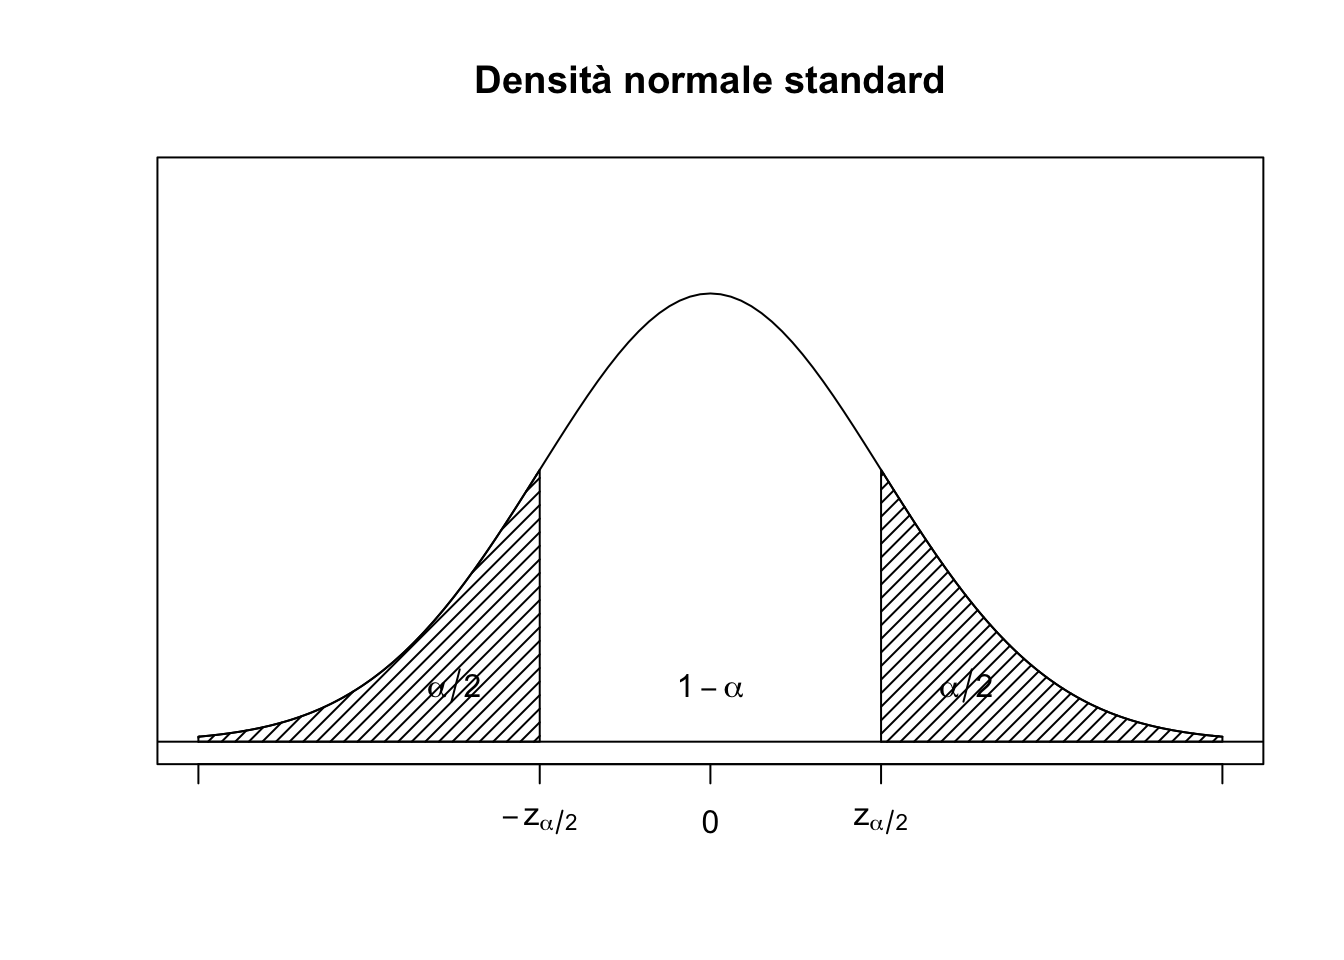
\includegraphics{statistics-project_files/figure-latex/normale-standard-1} 

}

\caption{Densità normale standard}\label{fig:normale-standard}
\end{figure}

\section{Intervalli di fiducia approssimati per la popolazione
geometrica}\label{intervalli-di-fiducia-approssimati-per-la-popolazione-geometrica}

Nel caso della popolazione geometrica il valore medio e la varianza
della popolazione, e il valore medio e la varianza della media
campionaria hanno valori \[E(X) = 1/p  \quad Var(X) = (1-p) / p^2\]
\[E(\overline{X_n}) = 1/p \quad Var(\overline X_n) = (1-p) / (n p^2)\]

per il teorema centrale di convergenza la variabile aleatoria
\[Z_n = \frac{\overline X - E(\overline{X_n})}{Var(\overline X_n)} = \frac{\overline{X} - 1/p}{\sqrt{(1-p) / (n p^2)}} = \frac{p\overline{X} -1}{p} \frac{p\sqrt{n}}{\sqrt{1-p}} = \sqrt{n} \frac{p\overline{X} -1}{\sqrt{1-p}}\]
converge in distribuzione a una normale standard.

La disuguaglianza
\[-z_{\alpha/2} < \sqrt{n} \frac{p\overline{x} -1}{\sqrt{1-p}} < z_{\alpha/2}\]
è equivalente alla disequazione di secondo grado
\[ \left[ \sqrt{n} \frac{p\overline{x} -1}{\sqrt{1-p}} \right]^2 < z_{\alpha/2}\]

espressa nel seguito in forma canonica
\[n\overline{x}^2 p^2 +p(z_{\alpha/2}^2 -2n\overline{x_n}) + n -z_{\alpha/2}^2 < 0\]

La soluzioni della disequazione sono interne all'intervallo formato
dalle radici del polinomio. Tali radici possono essere calcolate
esplicitamente o mediante la funzione \emph{polyroot}.

La seguente funzione consente di calcolare l'intervallo di confidenza
per il parametro \(p\) di una distribuzione geometrica dati in input il
grado \(1-\alpha\), la lunghezza del campione e la media campionaria.

\begin{Shaded}
\begin{Highlighting}[]
\NormalTok{intervalloDiConfidenza <-}\StringTok{ }\ControlFlowTok{function}\NormalTok{(grado, lunghezzaCampione, mediaCampionaria) \{}
\NormalTok{  alpha <-}\StringTok{ }\DecValTok{1} \OperatorTok{-}\StringTok{ }\NormalTok{grado}
\NormalTok{  zalpha <-}\StringTok{ }\KeywordTok{qnorm}\NormalTok{(}\DecValTok{1} \OperatorTok{-}\StringTok{ }\NormalTok{alpha }\OperatorTok{/}\StringTok{ }\DecValTok{2}\NormalTok{, }\DataTypeTok{mean =} \DecValTok{0}\NormalTok{, }\DataTypeTok{sd =} \DecValTok{1}\NormalTok{)}
\NormalTok{  a2 <-}\StringTok{ }\NormalTok{lunghezzaCampione }\OperatorTok{*}\StringTok{ }\NormalTok{mediaCampionaria}\OperatorTok{^}\DecValTok{2}
\NormalTok{  a1 <-}\StringTok{ }\NormalTok{zalpha}\OperatorTok{^}\DecValTok{2} \OperatorTok{-}\StringTok{ }\DecValTok{2} \OperatorTok{*}\StringTok{ }\NormalTok{lunghezzaCampione }\OperatorTok{*}\StringTok{ }\NormalTok{mediaCampionaria}
\NormalTok{  a0 <-}\StringTok{ }\NormalTok{lunghezzaCampione }\OperatorTok{-}\StringTok{ }\NormalTok{zalpha}\OperatorTok{^}\DecValTok{2}
\NormalTok{  radici <-}\StringTok{ }\KeywordTok{polyroot}\NormalTok{(}\KeywordTok{c}\NormalTok{(a0,a1,a2))}
\NormalTok{  radici}
\NormalTok{\}}
\end{Highlighting}
\end{Shaded}

Il seguente codice definisce una variabile contenente i dati del
campione e calcola l'intervallo di confidenza di grado
\(1-\alpha = 0.95\) per \(p\).

\begin{Shaded}
\begin{Highlighting}[]
\NormalTok{campione <-}\StringTok{ }\KeywordTok{c}\NormalTok{(}\DecValTok{2}\NormalTok{, }\DecValTok{1}\NormalTok{, }\DecValTok{1}\NormalTok{, }\DecValTok{3}\NormalTok{, }\DecValTok{1}\NormalTok{, }\DecValTok{3}\NormalTok{, }\DecValTok{4}\NormalTok{, }\DecValTok{5}\NormalTok{, }\DecValTok{1}\NormalTok{, }\DecValTok{1}\NormalTok{, }\DecValTok{1}\NormalTok{, }\DecValTok{1}\NormalTok{, }\DecValTok{4}\NormalTok{, }\DecValTok{2}\NormalTok{, }\DecValTok{2}\NormalTok{, }\DecValTok{2}\NormalTok{, }\DecValTok{4}\NormalTok{, }\DecValTok{3}\NormalTok{, }\DecValTok{3}\NormalTok{, }\DecValTok{1}\NormalTok{, }
         \DecValTok{1}\NormalTok{, }\DecValTok{1}\NormalTok{, }\DecValTok{2}\NormalTok{, }\DecValTok{2}\NormalTok{, }\DecValTok{1}\NormalTok{, }\DecValTok{1}\NormalTok{, }\DecValTok{1}\NormalTok{, }\DecValTok{2}\NormalTok{, }\DecValTok{3}\NormalTok{, }\DecValTok{6}\NormalTok{, }\DecValTok{3}\NormalTok{, }\DecValTok{1}\NormalTok{, }\DecValTok{6}\NormalTok{, }\DecValTok{1}\NormalTok{, }\DecValTok{1}\NormalTok{, }\DecValTok{2}\NormalTok{, }\DecValTok{1}\NormalTok{, }\DecValTok{4}\NormalTok{, }\DecValTok{1}\NormalTok{, }\DecValTok{1}\NormalTok{, }
         \DecValTok{4}\NormalTok{, }\DecValTok{3}\NormalTok{, }\DecValTok{2}\NormalTok{, }\DecValTok{1}\NormalTok{, }\DecValTok{4}\NormalTok{, }\DecValTok{6}\NormalTok{, }\DecValTok{7}\NormalTok{, }\DecValTok{2}\NormalTok{, }\DecValTok{1}\NormalTok{, }\DecValTok{1}\NormalTok{, }\DecValTok{3}\NormalTok{, }\DecValTok{1}\NormalTok{, }\DecValTok{1}\NormalTok{, }\DecValTok{4}\NormalTok{, }\DecValTok{1}\NormalTok{, }\DecValTok{1}\NormalTok{, }\DecValTok{4}\NormalTok{, }\DecValTok{1}\NormalTok{, }\DecValTok{4}\NormalTok{, }\DecValTok{1}\NormalTok{, }
         \DecValTok{2}\NormalTok{, }\DecValTok{1}\NormalTok{, }\DecValTok{1}\NormalTok{, }\DecValTok{1}\NormalTok{, }\DecValTok{4}\NormalTok{, }\DecValTok{2}\NormalTok{, }\DecValTok{1}\NormalTok{, }\DecValTok{2}\NormalTok{, }\DecValTok{3}\NormalTok{, }\DecValTok{2}\NormalTok{, }\DecValTok{2}\NormalTok{, }\DecValTok{1}\NormalTok{, }\DecValTok{2}\NormalTok{, }\DecValTok{1}\NormalTok{, }\DecValTok{2}\NormalTok{, }\DecValTok{1}\NormalTok{, }\DecValTok{2}\NormalTok{, }\DecValTok{2}\NormalTok{, }\DecValTok{6}\NormalTok{, }\DecValTok{5}\NormalTok{, }
         \DecValTok{6}\NormalTok{, }\DecValTok{2}\NormalTok{, }\DecValTok{6}\NormalTok{, }\DecValTok{2}\NormalTok{, }\DecValTok{3}\NormalTok{, }\DecValTok{2}\NormalTok{, }\DecValTok{2}\NormalTok{, }\DecValTok{2}\NormalTok{, }\DecValTok{4}\NormalTok{, }\DecValTok{1}\NormalTok{, }\DecValTok{1}\NormalTok{, }\DecValTok{1}\NormalTok{, }\DecValTok{1}\NormalTok{, }\DecValTok{2}\NormalTok{, }\DecValTok{3}\NormalTok{, }\DecValTok{9}\NormalTok{, }\DecValTok{3}\NormalTok{, }\DecValTok{1}\NormalTok{, }\DecValTok{2}\NormalTok{, }\DecValTok{1}\NormalTok{)}

\NormalTok{intervallo <-}\StringTok{ }\KeywordTok{intervalloDiConfidenza}\NormalTok{(}\DataTypeTok{grado =} \FloatTok{0.95}\NormalTok{, }
                                     \DataTypeTok{lunghezzaCampione =} \KeywordTok{length}\NormalTok{(campione), }
                                     \DataTypeTok{mediaCampionaria =} \KeywordTok{mean}\NormalTok{(campione))}
\end{Highlighting}
\end{Shaded}

L'intervallo di confidenza di grado \(1-\alpha = 0.95\) per il parametro
\(p\) calcolato è

(0.358744314001264-0i, 0.48536350162446+0i)

Da notare che la stima puntuale di valore 0.4255319 risulta interna
all'intervallo.

\section{Differenza tra valori medi}\label{differenza-tra-valori-medi}

Siano \(X_1,..,X_{n}\) e \(Y_1,..,Y_{m}\) due campioni casuali di
ampiezza \(n_1\) e \(n_2\) estratti da due popolazioni geometriche con
parametri \(p_1\) e \(p_2\) rispettivamente. Vogliamo determinare un
intervallo di confidenza di grado \(1-\alpha\) per la differenza
\(p_1 - p_2\).

Essendo
\[E(\overline{X_{n_1}}-\overline{Y_{n_2}}) = \frac{1}{p_1} - \frac{1}{p_2}\]

\[Var(\overline{X_{n_1}}-\overline{Y_{n_2}}) = \frac{1-p_1}{n_1 p_1^2} + \frac{1-p_2}{n_2 p_2^2}\]

allora per il teorema centrale di convergenza la variabile aleatoria

\[\frac{\overline{X_{n_1}} - \overline{Y_{n_2}} - \left( \frac{1}{p_1} - \frac{1}{p_2} \right)}{\sqrt{\frac{1-p_1}{n_1 p_1^2} + \frac{1-p_2}{n_2 p_2^2}}}\]

converge in distribuzione alla variabile aleatoria normale standard
\(Z \sim \mathcal{N}(0, 1)\).

Inoltre essendo

\[lim_{n \to + \infty} E[\overline{X_{n_1}}(\overline{X_{n_1}} - 1)] = \frac{1-p_1}{p_1^2}\]
\[lim_{n \to + \infty} E[\overline{Y_{n_2}}(\overline{Y_{n_2}} -1)] = \frac{1-p_2}{p_2^2}\]

Per campioni sufficientemente grandi

\[P\left( -z_{\alpha/2} < \frac{\overline{X_{n_1}} - \overline{Y_{n_2}} - \left( \frac{1}{p_1} - \frac{1}{p_2} \right)}{\sqrt{\frac{\overline{X_{n_1}}(\overline{X_{n_1}} - 1)}{n_1} + \frac{\overline{Y_{n_2}}(\overline{Y_{n_2}} - 1)}{n_1}}} < z_{\alpha/2} \right) \backsimeq 1 - \alpha\]
La disuguaglianza
\[-z_{\alpha/2} < \frac{\overline{x_{n_1}} - \overline{y_{n_2}} - \left( \frac{1}{p_1} - \frac{1}{p_2} \right)}{\sqrt{\frac{\overline{x_{n_1}}(\overline{x_{n_1}} - 1)}{n_1} + \frac{\overline{y_{n_2}}(\overline{y_{n_2}} - 1)}{n_1}}} < z_{\alpha/2}\]

è equivalente a

\[ \overline{x_{n_1}} - \overline{y_{n_2}}  - z_{\alpha/2} \sqrt{\frac{\overline{x_{n_1}}(\overline{x_{n_1}} - 1)}{n_1} + \frac{\overline{y_{n_2}}(\overline{y_{n_2}} - 1)}{n_1}}<  \left( \frac{1}{p_1} - \frac{1}{p_2} \right)\]

\[ \left( \frac{1}{p_1} - \frac{1}{p_2} \right) < \overline{x_{n_1}} - \overline{y_{n_2}}  + z_{\alpha/2} \sqrt{\frac{\overline{x_{n_1}}(\overline{x_{n_1}} - 1)}{n_1} + \frac{\overline{y_{n_2}}(\overline{y_{n_2}} - 1)}{n_1}}\]
La seguente funzione consente di calcolare l'intervallo di confidenza
per la differenza dei valori medi dati in input il grado \(1-\alpha\),
la lunghezza del primo campione e del secondo campione e la media
campionaria del primo e del secondo campione.

\begin{Shaded}
\begin{Highlighting}[]
\NormalTok{differenzeValoriMedi <-}\StringTok{ }\ControlFlowTok{function}\NormalTok{(grado, n1, n2, m1, m2) \{}
\NormalTok{  alpha <-}\StringTok{ }\DecValTok{1} \OperatorTok{-}\StringTok{ }\NormalTok{grado}
\NormalTok{  delta <-}\StringTok{ }\NormalTok{m1 }\OperatorTok{*}\StringTok{ }\NormalTok{(m1 }\OperatorTok{-}\StringTok{ }\DecValTok{1}\NormalTok{) }\OperatorTok{/}\StringTok{ }\NormalTok{n1 }\OperatorTok{+}\StringTok{ }\NormalTok{m2 }\OperatorTok{*}\StringTok{ }\NormalTok{(m2 }\OperatorTok{-}\StringTok{ }\DecValTok{1}\NormalTok{) }\OperatorTok{/}\StringTok{ }\NormalTok{n2}
\NormalTok{  radice <-}\StringTok{ }\KeywordTok{sqrt}\NormalTok{(delta)}
\NormalTok{  a <-}\StringTok{ }\NormalTok{m1 }\OperatorTok{-}\StringTok{ }\NormalTok{m2}
\NormalTok{  b <-}\StringTok{ }\KeywordTok{qnorm}\NormalTok{(}\DecValTok{1} \OperatorTok{-}\StringTok{ }\NormalTok{alpha }\OperatorTok{/}\StringTok{ }\DecValTok{2}\NormalTok{, }\DataTypeTok{mean =} \DecValTok{0}\NormalTok{, }\DataTypeTok{sd =} \DecValTok{1}\NormalTok{) }\OperatorTok{*}\StringTok{ }\NormalTok{radice}
\NormalTok{  left <-}\StringTok{  }\NormalTok{a }\OperatorTok{-}\StringTok{ }\NormalTok{b}
\NormalTok{  right <-}\StringTok{ }\NormalTok{a }\OperatorTok{+}\StringTok{ }\NormalTok{b}
  \KeywordTok{return}\NormalTok{(}\KeywordTok{c}\NormalTok{(left, right))}
\NormalTok{\}}
\end{Highlighting}
\end{Shaded}

\textbf{Interpretazione intervallo}

\begin{itemize}
\item
  Se gli estremi dell'intervallo sono entrambi positivi allora il valore
  medio della prima popolazione è maggiore del valore medio della
  seconda popolazione.
\item
  Se gli estremi dell'intervallo sono entrambi negativi allora il valore
  medio della prima popolazione è minore del valore medio della seconda
  popolazione.
\item
  Altrimenti esiste la possibilità che i valori medi siano uguali,
  quindi non è possibile dire quale sia maggiore.
\end{itemize}

Il seguente codice definisce due campione e calcola l'intervallo di
confidenza di grado \(1-\alpha = 0.99\) per le differenze dei valori
medi.

\begin{Shaded}
\begin{Highlighting}[]
\CommentTok{#campione1 <- rgeom(150, prob = 0.3) + 1}
\NormalTok{campione1 <-}\StringTok{ }\KeywordTok{c}\NormalTok{(}\DecValTok{2}\NormalTok{, }\DecValTok{4}\NormalTok{, }\DecValTok{7}\NormalTok{, }\DecValTok{5}\NormalTok{, }\DecValTok{2}\NormalTok{, }\DecValTok{2}\NormalTok{, }\DecValTok{1}\NormalTok{, }\DecValTok{2}\NormalTok{, }\DecValTok{6}\NormalTok{, }\DecValTok{5}\NormalTok{, }\DecValTok{3}\NormalTok{, }\DecValTok{2}\NormalTok{, }\DecValTok{6}\NormalTok{, }\DecValTok{1}\NormalTok{, }\DecValTok{4}\NormalTok{, }\DecValTok{1}\NormalTok{, }\DecValTok{5}\NormalTok{, }\DecValTok{1}\NormalTok{, }\DecValTok{1}\NormalTok{, }\DecValTok{1}\NormalTok{, }
              \DecValTok{2}\NormalTok{, }\DecValTok{1}\NormalTok{, }\DecValTok{5}\NormalTok{, }\DecValTok{4}\NormalTok{, }\DecValTok{9}\NormalTok{, }\DecValTok{6}\NormalTok{, }\DecValTok{3}\NormalTok{, }\DecValTok{5}\NormalTok{, }\DecValTok{3}\NormalTok{, }\DecValTok{4}\NormalTok{, }\DecValTok{3}\NormalTok{, }\DecValTok{1}\NormalTok{, }\DecValTok{6}\NormalTok{, }\DecValTok{1}\NormalTok{, }\DecValTok{3}\NormalTok{, }\DecValTok{1}\NormalTok{, }\DecValTok{1}\NormalTok{, }\DecValTok{4}\NormalTok{, }\DecValTok{3}\NormalTok{, }\DecValTok{1}\NormalTok{, }
              \DecValTok{3}\NormalTok{, }\DecValTok{1}\NormalTok{, }\DecValTok{1}\NormalTok{, }\DecValTok{1}\NormalTok{, }\DecValTok{1}\NormalTok{, }\DecValTok{4}\NormalTok{, }\DecValTok{2}\NormalTok{, }\DecValTok{3}\NormalTok{, }\DecValTok{6}\NormalTok{, }\DecValTok{1}\NormalTok{, }\DecValTok{3}\NormalTok{, }\DecValTok{1}\NormalTok{, }\DecValTok{3}\NormalTok{, }\DecValTok{7}\NormalTok{, }\DecValTok{12}\NormalTok{, }\DecValTok{5}\NormalTok{, }\DecValTok{5}\NormalTok{, }\DecValTok{3}\NormalTok{, }\DecValTok{1}\NormalTok{, }\DecValTok{4}\NormalTok{, }
              \DecValTok{2}\NormalTok{, }\DecValTok{3}\NormalTok{, }\DecValTok{1}\NormalTok{, }\DecValTok{7}\NormalTok{, }\DecValTok{4}\NormalTok{, }\DecValTok{3}\NormalTok{, }\DecValTok{5}\NormalTok{, }\DecValTok{1}\NormalTok{, }\DecValTok{3}\NormalTok{, }\DecValTok{11}\NormalTok{, }\DecValTok{9}\NormalTok{, }\DecValTok{1}\NormalTok{, }\DecValTok{3}\NormalTok{, }\DecValTok{4}\NormalTok{, }\DecValTok{1}\NormalTok{, }\DecValTok{2}\NormalTok{, }\DecValTok{4}\NormalTok{, }\DecValTok{2}\NormalTok{, }\DecValTok{1}\NormalTok{, }\DecValTok{4}\NormalTok{, }
              \DecValTok{4}\NormalTok{, }\DecValTok{2}\NormalTok{, }\DecValTok{5}\NormalTok{, }\DecValTok{8}\NormalTok{, }\DecValTok{12}\NormalTok{, }\DecValTok{5}\NormalTok{, }\DecValTok{2}\NormalTok{, }\DecValTok{1}\NormalTok{, }\DecValTok{1}\NormalTok{, }\DecValTok{6}\NormalTok{, }\DecValTok{2}\NormalTok{, }\DecValTok{2}\NormalTok{, }\DecValTok{5}\NormalTok{, }\DecValTok{1}\NormalTok{, }\DecValTok{4}\NormalTok{, }\DecValTok{7}\NormalTok{, }\DecValTok{1}\NormalTok{, }\DecValTok{3}\NormalTok{, }\DecValTok{1}\NormalTok{, }\DecValTok{2}\NormalTok{, }
              \DecValTok{2}\NormalTok{, }\DecValTok{2}\NormalTok{, }\DecValTok{4}\NormalTok{, }\DecValTok{4}\NormalTok{, }\DecValTok{3}\NormalTok{, }\DecValTok{4}\NormalTok{, }\DecValTok{2}\NormalTok{, }\DecValTok{4}\NormalTok{, }\DecValTok{1}\NormalTok{, }\DecValTok{5}\NormalTok{, }\DecValTok{1}\NormalTok{, }\DecValTok{2}\NormalTok{, }\DecValTok{1}\NormalTok{, }\DecValTok{3}\NormalTok{, }\DecValTok{4}\NormalTok{, }\DecValTok{1}\NormalTok{, }\DecValTok{6}\NormalTok{, }\DecValTok{1}\NormalTok{, }\DecValTok{2}\NormalTok{, }\DecValTok{3}\NormalTok{,}
              \DecValTok{12}\NormalTok{, }\DecValTok{2}\NormalTok{, }\DecValTok{3}\NormalTok{, }\DecValTok{4}\NormalTok{, }\DecValTok{13}\NormalTok{, }\DecValTok{1}\NormalTok{, }\DecValTok{1}\NormalTok{, }\DecValTok{2}\NormalTok{, }\DecValTok{3}\NormalTok{, }\DecValTok{3}\NormalTok{, }\DecValTok{3}\NormalTok{, }\DecValTok{4}\NormalTok{, }\DecValTok{2}\NormalTok{, }\DecValTok{9}\NormalTok{, }\DecValTok{1}\NormalTok{, }\DecValTok{5}\NormalTok{, }\DecValTok{1}\NormalTok{, }\DecValTok{2}\NormalTok{, }\DecValTok{1}\NormalTok{, }\DecValTok{5}\NormalTok{, }
              \DecValTok{3}\NormalTok{, }\DecValTok{5}\NormalTok{, }\DecValTok{8}\NormalTok{, }\DecValTok{1}\NormalTok{, }\DecValTok{9}\NormalTok{, }\DecValTok{9}\NormalTok{, }\DecValTok{4}\NormalTok{, }\DecValTok{2}\NormalTok{, }\DecValTok{1}\NormalTok{, }\DecValTok{5}\NormalTok{)}

\CommentTok{#campione2 <- rgeom(100, prob = 0.6) + 1}
\NormalTok{campione2 <-}\StringTok{ }\KeywordTok{c}\NormalTok{(}\DecValTok{3}\NormalTok{, }\DecValTok{1}\NormalTok{, }\DecValTok{1}\NormalTok{, }\DecValTok{1}\NormalTok{, }\DecValTok{2}\NormalTok{, }\DecValTok{2}\NormalTok{, }\DecValTok{2}\NormalTok{, }\DecValTok{1}\NormalTok{, }\DecValTok{1}\NormalTok{, }\DecValTok{1}\NormalTok{, }\DecValTok{3}\NormalTok{, }\DecValTok{1}\NormalTok{, }\DecValTok{1}\NormalTok{, }\DecValTok{1}\NormalTok{, }\DecValTok{4}\NormalTok{, }\DecValTok{2}\NormalTok{, }\DecValTok{3}\NormalTok{, }\DecValTok{2}\NormalTok{, }\DecValTok{1}\NormalTok{, }\DecValTok{4}\NormalTok{, }
               \DecValTok{4}\NormalTok{, }\DecValTok{4}\NormalTok{, }\DecValTok{1}\NormalTok{, }\DecValTok{1}\NormalTok{, }\DecValTok{1}\NormalTok{, }\DecValTok{1}\NormalTok{, }\DecValTok{3}\NormalTok{, }\DecValTok{1}\NormalTok{, }\DecValTok{1}\NormalTok{, }\DecValTok{2}\NormalTok{, }\DecValTok{1}\NormalTok{, }\DecValTok{1}\NormalTok{, }\DecValTok{1}\NormalTok{, }\DecValTok{2}\NormalTok{, }\DecValTok{1}\NormalTok{, }\DecValTok{2}\NormalTok{, }\DecValTok{2}\NormalTok{, }\DecValTok{1}\NormalTok{, }\DecValTok{1}\NormalTok{, }\DecValTok{1}\NormalTok{, }
               \DecValTok{1}\NormalTok{, }\DecValTok{2}\NormalTok{, }\DecValTok{1}\NormalTok{, }\DecValTok{1}\NormalTok{, }\DecValTok{2}\NormalTok{, }\DecValTok{1}\NormalTok{, }\DecValTok{1}\NormalTok{, }\DecValTok{1}\NormalTok{, }\DecValTok{1}\NormalTok{, }\DecValTok{1}\NormalTok{, }\DecValTok{1}\NormalTok{, }\DecValTok{1}\NormalTok{, }\DecValTok{1}\NormalTok{, }\DecValTok{1}\NormalTok{, }\DecValTok{1}\NormalTok{, }\DecValTok{1}\NormalTok{, }\DecValTok{2}\NormalTok{, }\DecValTok{1}\NormalTok{, }\DecValTok{1}\NormalTok{, }\DecValTok{6}\NormalTok{, }
               \DecValTok{1}\NormalTok{, }\DecValTok{1}\NormalTok{, }\DecValTok{2}\NormalTok{, }\DecValTok{3}\NormalTok{, }\DecValTok{2}\NormalTok{, }\DecValTok{4}\NormalTok{, }\DecValTok{2}\NormalTok{, }\DecValTok{1}\NormalTok{, }\DecValTok{1}\NormalTok{, }\DecValTok{2}\NormalTok{, }\DecValTok{1}\NormalTok{, }\DecValTok{1}\NormalTok{, }\DecValTok{4}\NormalTok{, }\DecValTok{6}\NormalTok{, }\DecValTok{1}\NormalTok{, }\DecValTok{2}\NormalTok{, }\DecValTok{1}\NormalTok{, }\DecValTok{1}\NormalTok{, }\DecValTok{1}\NormalTok{, }\DecValTok{1}\NormalTok{, }
               \DecValTok{2}\NormalTok{, }\DecValTok{2}\NormalTok{, }\DecValTok{3}\NormalTok{, }\DecValTok{1}\NormalTok{, }\DecValTok{1}\NormalTok{, }\DecValTok{2}\NormalTok{, }\DecValTok{1}\NormalTok{, }\DecValTok{4}\NormalTok{, }\DecValTok{1}\NormalTok{, }\DecValTok{1}\NormalTok{, }\DecValTok{1}\NormalTok{, }\DecValTok{1}\NormalTok{, }\DecValTok{1}\NormalTok{, }\DecValTok{1}\NormalTok{, }\DecValTok{2}\NormalTok{, }\DecValTok{1}\NormalTok{, }\DecValTok{6}\NormalTok{, }\DecValTok{1}\NormalTok{, }\DecValTok{2}\NormalTok{, }\DecValTok{1}\NormalTok{)}

\NormalTok{intervallo <-}\StringTok{ }\KeywordTok{differenzeValoriMedi}\NormalTok{(}\DataTypeTok{grado =} \FloatTok{0.99}\NormalTok{, }
                               \DataTypeTok{n1 =} \KeywordTok{length}\NormalTok{(campione1), }\DataTypeTok{n2 =} \KeywordTok{length}\NormalTok{(campione2), }
                               \DataTypeTok{m1 =} \KeywordTok{mean}\NormalTok{(campione1), }\DataTypeTok{m2 =} \KeywordTok{mean}\NormalTok{(campione2))}
\end{Highlighting}
\end{Shaded}

L'intervallo ottenuto è

(1.0797592, 2.4269075)

Essendo gli estremi ottenuti entrambi positivi ne consegue che la media
della prima popolazione è maggiore della media della seconda
popolazione.

\chapter{Verifica delle ipotesi}\label{verifica-delle-ipotesi}

Il test di verifica delle ipotesi è un test che mira a verificare la
bontà di un'ipotesi rappresentante un'affermazione su un parametro non
noto della distribuzione che descrive la popolazione.

L'ipotesi da verificare tramite il test è detta ipotesi nulla \(H_0\),
se l'ipotesi nulla non può essere accettata allora viene accettata
un'ipotesi alternativa \(H_1\) espressa in contrapposizione all'ipotesi
nulla.

Se \(\Theta_0\) e \(\Theta_1\) sono due sottoinsiemi disgiunti dello
spazio dei parametri \(\Theta\) allora l'ipotesi nulla e alternativa
possono essere espresse come

\[H_0: \theta \in \Theta_0 \quad H_1: \theta \in \Theta_1\]

Se l'ipotesi specifica completamente la funzione di probabilità o
densità di probabilità allora l'ipotesi è detta semplice, altrimenti è
detta composta.

La verifica del test può incorrere in due tipologie di errore:

\begin{itemize}
\item
  Errore di tipo I - rifiuto dell'ipotesi nulla quando l'ipotesi è vera
\item
  Errore di tipo II - accettazione dell'ipotesi nulla quando l'ipotesi è
  falsa
\end{itemize}

Se per effettuare il test vengono utilizzati campioni di ampiezza fissa
allora, in genere, al diminuire della probabilità di commettere un
errore di un dato tipo aumenta la probabilità di commettere un errore
dell'altro tipo.

Di conseguenza, se l'errore di tipo I è più grave dell'errore di tipo
II, si fissa la probabilità di commettere errori di tipo I e si
minimizza la probabilità di commettere errori di tipo II, altrimenti il
contrario.

In genere le probabilità di errore scelte sono di 0.5 (test
statisticamente significativo), 0.01 (test statisticamente molto
significativo) e 0.001 (test statisticamente estremamente
significativo).

Nel seguito verranno mostrati test di verifica delle ipotesi unilaterali
e bilaterali con una probabilità \(\alpha\) di commettere errori di tipo
I sul valore medio di una distribuzione geometrica nel caso in cui la
varianza sia nota.

In modo analogo a quanto fatto per il calcolo degli intervalli di
fiducia approssimati, utilizzeremo una variabile pivot che converge in
distribuzione alla normale standard.

Infatti se \(X_1,\dots,X_n\) è un campione casuale estratto da una
popolazione geometrica con valore medio \(\mu\) e varianza \(\sigma^2\)
allora la variabile aleatoria

\[Y_n = \frac{\overline X - \mu}{\sigma / \sqrt{n}} \]

converge in distribuzione alla variabile normale standard
\(Z \sim \mathcal{N}(0, 1)\).

\section{Test bilaterale
approssimato}\label{test-bilaterale-approssimato}

Se \((x_1,\dots,x_n)\) è un campione osservato di ampiezza \(n\)
estratto da una popolazione geometrica con varianza nota \(\sigma^2\) e
se consideriamo le ipotesi:

\[H_0 : \mu = \mu_0 \quad H_1 : \mu \neq \mu_0\]

allora il test bilaterale \(\Phi\) di misura \(\alpha\) per le ipotesi
è:

\emph{Accettiamo l'ipotesi \(H_0\) se}
\[-z_{\alpha/2} < \frac{\overline x - \mu_0}{\sigma / \sqrt{n}} < z_{\alpha/2}\]

\emph{Rifiutiamo l'ipotesi \(H_0\) se}
\[\frac{\overline x - \mu_0}{\sigma / \sqrt{n}} > z_{\alpha/2} \quad \text{oppure} \quad \frac{\overline x - \mu_0}{\sigma /  \sqrt{n}} < - z_{\alpha/2} \]

dove \(-z_{\alpha/2}\) e \(z_{\alpha/2}\) sono tali che
\[P(Z < -z_{\alpha/2}) = P(Z > z_{\alpha/2}) = \frac{\alpha}{2}\]

In figura \ref{fig:verifica-ipotesi-bilaterale} è rappresentata una
densità normale standard e sono mostrate le regioni di rifiuto e
accettazione per il test bilaterale.

\begin{figure}

{\centering 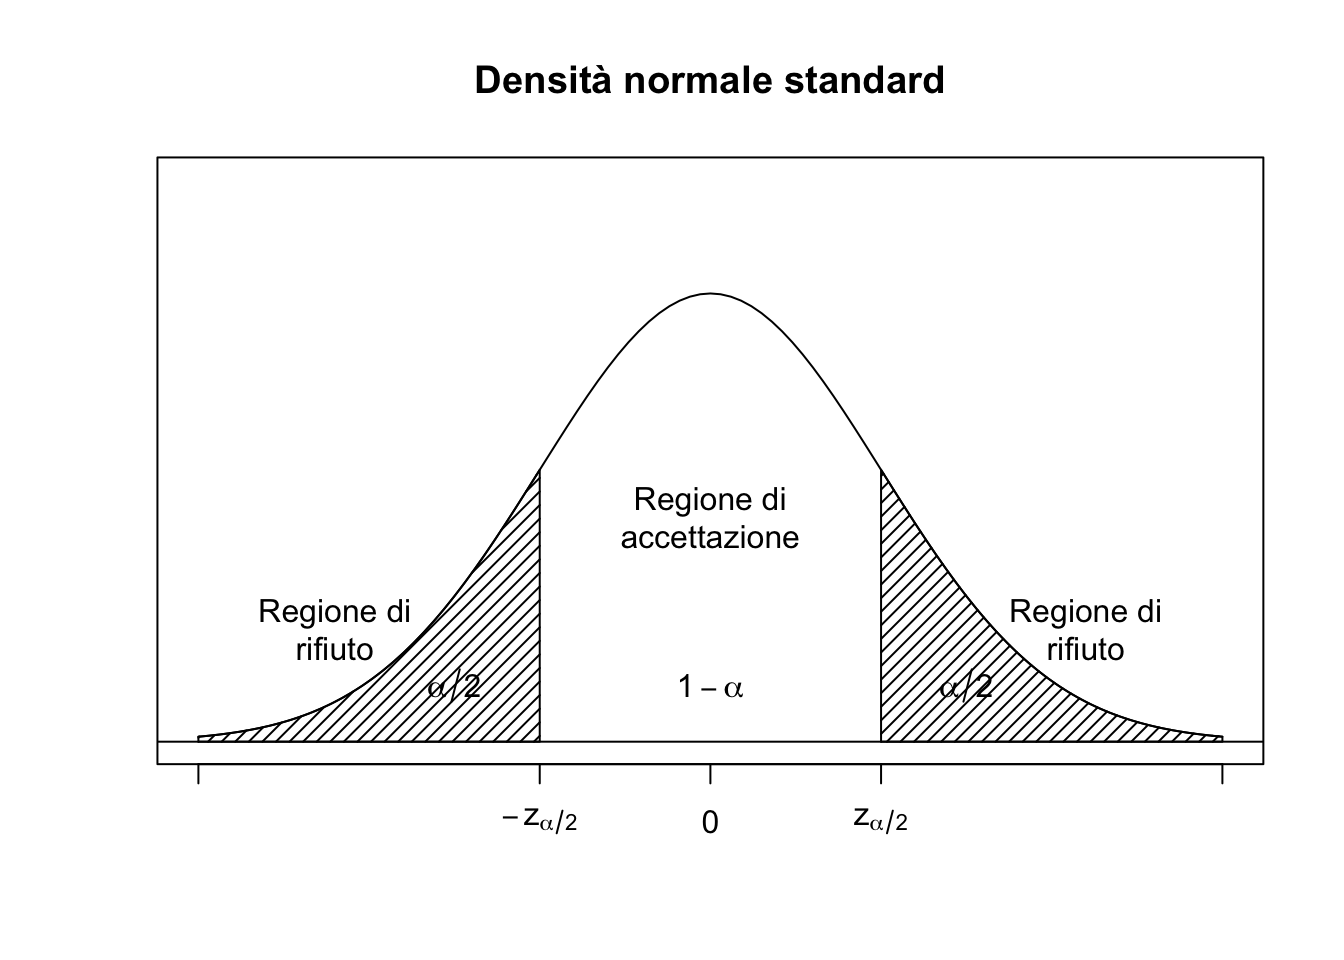
\includegraphics{statistics-project_files/figure-latex/verifica-ipotesi-bilaterale-1} 

}

\caption{Densità normale standard}\label{fig:verifica-ipotesi-bilaterale}
\end{figure}

La seguente funzione effettua il test bilaterale approssimato. La
funzione prende in input la media e la deviazione standard della
popolazione, la media campionaria e la misura \(\alpha\).

\begin{Shaded}
\begin{Highlighting}[]
\NormalTok{testBilaterale <-}\StringTok{ }\ControlFlowTok{function}\NormalTok{(media, deviazioneStandard, mediaCampionaria, n, alpha) \{}
\NormalTok{  zAlphaMezzi <-}\StringTok{ }\KeywordTok{qnorm}\NormalTok{(}\DecValTok{1} \OperatorTok{-}\StringTok{ }\NormalTok{alpha }\OperatorTok{/}\StringTok{ }\DecValTok{2}\NormalTok{, }\DataTypeTok{mean =} \DecValTok{0}\NormalTok{, }\DataTypeTok{sd =} \DecValTok{1}\NormalTok{)}
\NormalTok{  valore <-}\StringTok{ }\NormalTok{(mediaCampionaria }\OperatorTok{-}\StringTok{ }\NormalTok{media) }\OperatorTok{/}\StringTok{ }\NormalTok{(deviazioneStandard }\OperatorTok{/}\StringTok{ }\KeywordTok{sqrt}\NormalTok{(n))}
  \OperatorTok{-}\NormalTok{zAlphaMezzi }\OperatorTok{<}\StringTok{ }\NormalTok{valore }\OperatorTok{&&}\StringTok{ }\NormalTok{valore }\OperatorTok{<}\StringTok{ }\NormalTok{zAlphaMezzi}
\NormalTok{\}}
\end{Highlighting}
\end{Shaded}

Il seguente codice effettua il test bilaterale sul valore medio
utilizzando un campione che si ritiene estratto da una popolazione
geometrica di parametro \(p = 0.4\). Vengono quindi calcolate la media e
la deviazione standard della popolazione e viene poi invocata la
precedente funzione per ottenere il risultato del test.

\begin{Shaded}
\begin{Highlighting}[]
\NormalTok{p <-}\StringTok{ }\FloatTok{0.4}
\NormalTok{media <-}\StringTok{ }\DecValTok{1} \OperatorTok{/}\StringTok{ }\NormalTok{p}
\NormalTok{varianza <-}\StringTok{ }\NormalTok{(}\DecValTok{1} \OperatorTok{-}\StringTok{ }\NormalTok{p) }\OperatorTok{/}\StringTok{ }\NormalTok{p}\OperatorTok{^}\DecValTok{2}
\NormalTok{deviazioneStandard <-}\StringTok{ }\KeywordTok{sqrt}\NormalTok{(varianza)}

\CommentTok{#campione <- rgeom(100, prob = 0.4) + 1}
\NormalTok{campione <-}\StringTok{ }\KeywordTok{c}\NormalTok{(}\DecValTok{2}\NormalTok{, }\DecValTok{1}\NormalTok{, }\DecValTok{1}\NormalTok{, }\DecValTok{3}\NormalTok{, }\DecValTok{1}\NormalTok{, }\DecValTok{3}\NormalTok{, }\DecValTok{4}\NormalTok{, }\DecValTok{5}\NormalTok{, }\DecValTok{1}\NormalTok{, }\DecValTok{1}\NormalTok{, }\DecValTok{1}\NormalTok{, }\DecValTok{1}\NormalTok{, }\DecValTok{4}\NormalTok{, }\DecValTok{2}\NormalTok{, }\DecValTok{2}\NormalTok{, }\DecValTok{2}\NormalTok{, }\DecValTok{4}\NormalTok{, }\DecValTok{3}\NormalTok{, }\DecValTok{3}\NormalTok{, }\DecValTok{1}\NormalTok{, }
              \DecValTok{1}\NormalTok{, }\DecValTok{1}\NormalTok{, }\DecValTok{2}\NormalTok{, }\DecValTok{2}\NormalTok{, }\DecValTok{1}\NormalTok{, }\DecValTok{1}\NormalTok{, }\DecValTok{1}\NormalTok{, }\DecValTok{2}\NormalTok{, }\DecValTok{3}\NormalTok{, }\DecValTok{6}\NormalTok{, }\DecValTok{3}\NormalTok{, }\DecValTok{1}\NormalTok{, }\DecValTok{6}\NormalTok{, }\DecValTok{1}\NormalTok{, }\DecValTok{1}\NormalTok{, }\DecValTok{2}\NormalTok{, }\DecValTok{1}\NormalTok{, }\DecValTok{4}\NormalTok{, }\DecValTok{1}\NormalTok{, }\DecValTok{1}\NormalTok{, }
              \DecValTok{4}\NormalTok{, }\DecValTok{3}\NormalTok{, }\DecValTok{2}\NormalTok{, }\DecValTok{1}\NormalTok{, }\DecValTok{4}\NormalTok{, }\DecValTok{6}\NormalTok{, }\DecValTok{7}\NormalTok{, }\DecValTok{2}\NormalTok{, }\DecValTok{1}\NormalTok{, }\DecValTok{1}\NormalTok{, }\DecValTok{3}\NormalTok{, }\DecValTok{1}\NormalTok{, }\DecValTok{1}\NormalTok{, }\DecValTok{4}\NormalTok{, }\DecValTok{1}\NormalTok{, }\DecValTok{1}\NormalTok{, }\DecValTok{4}\NormalTok{, }\DecValTok{1}\NormalTok{, }\DecValTok{4}\NormalTok{, }\DecValTok{1}\NormalTok{, }
              \DecValTok{2}\NormalTok{, }\DecValTok{1}\NormalTok{, }\DecValTok{1}\NormalTok{, }\DecValTok{1}\NormalTok{, }\DecValTok{4}\NormalTok{, }\DecValTok{2}\NormalTok{, }\DecValTok{1}\NormalTok{, }\DecValTok{2}\NormalTok{, }\DecValTok{3}\NormalTok{, }\DecValTok{2}\NormalTok{, }\DecValTok{2}\NormalTok{, }\DecValTok{1}\NormalTok{, }\DecValTok{2}\NormalTok{, }\DecValTok{1}\NormalTok{, }\DecValTok{2}\NormalTok{, }\DecValTok{1}\NormalTok{, }\DecValTok{2}\NormalTok{, }\DecValTok{2}\NormalTok{, }\DecValTok{6}\NormalTok{, }\DecValTok{5}\NormalTok{, }
              \DecValTok{6}\NormalTok{, }\DecValTok{2}\NormalTok{, }\DecValTok{6}\NormalTok{, }\DecValTok{2}\NormalTok{, }\DecValTok{3}\NormalTok{, }\DecValTok{2}\NormalTok{, }\DecValTok{2}\NormalTok{, }\DecValTok{2}\NormalTok{, }\DecValTok{4}\NormalTok{, }\DecValTok{1}\NormalTok{, }\DecValTok{1}\NormalTok{, }\DecValTok{1}\NormalTok{, }\DecValTok{1}\NormalTok{, }\DecValTok{2}\NormalTok{, }\DecValTok{3}\NormalTok{, }\DecValTok{9}\NormalTok{, }\DecValTok{3}\NormalTok{, }\DecValTok{1}\NormalTok{, }\DecValTok{2}\NormalTok{, }\DecValTok{1}\NormalTok{)}

\NormalTok{esito <-}\StringTok{ }\KeywordTok{testBilaterale}\NormalTok{(}\DataTypeTok{media =}\NormalTok{ media, }
                        \DataTypeTok{deviazioneStandard =}\NormalTok{ deviazioneStandard, }
                        \DataTypeTok{mediaCampionaria =} \KeywordTok{mean}\NormalTok{(campione), }
                        \DataTypeTok{n =} \KeywordTok{length}\NormalTok{(campione), }
                        \DataTypeTok{alpha =} \FloatTok{0.05}\NormalTok{)}
\end{Highlighting}
\end{Shaded}

Il test da esito positivo.

\section{Test unilaterale sinistro
approssimato}\label{test-unilaterale-sinistro-approssimato}

Se \((x_1,\dots,x_n)\) è un campione osservato di ampiezza \(n\)
estratto da una popolazione geometrica con varianza nota \(\sigma^2\) e
se consideriamo le ipotesi:

\[H_0 : \mu \le \mu_0 \quad H_1 : \mu > \mu_0\] allora il test
unilaterale sinistro \(\Phi\) di misura \(\alpha\) per le ipotesi è:

\emph{Accettiamo l'ipotesi \(H_0\) se}
\[\frac{\overline x - \mu_0}{\sigma / \sqrt{n}} < z_{\alpha}\]
\emph{Rifiutiamo l'ipotesi \(H_0\) se}
\[\frac{\overline x - \mu_0}{\sigma / \sqrt{n}} > z_{\alpha}\] dove
\(z_{\alpha}\) è tale che: \[P(Z > z_{\alpha}) = \alpha\]

\begin{figure}

{\centering 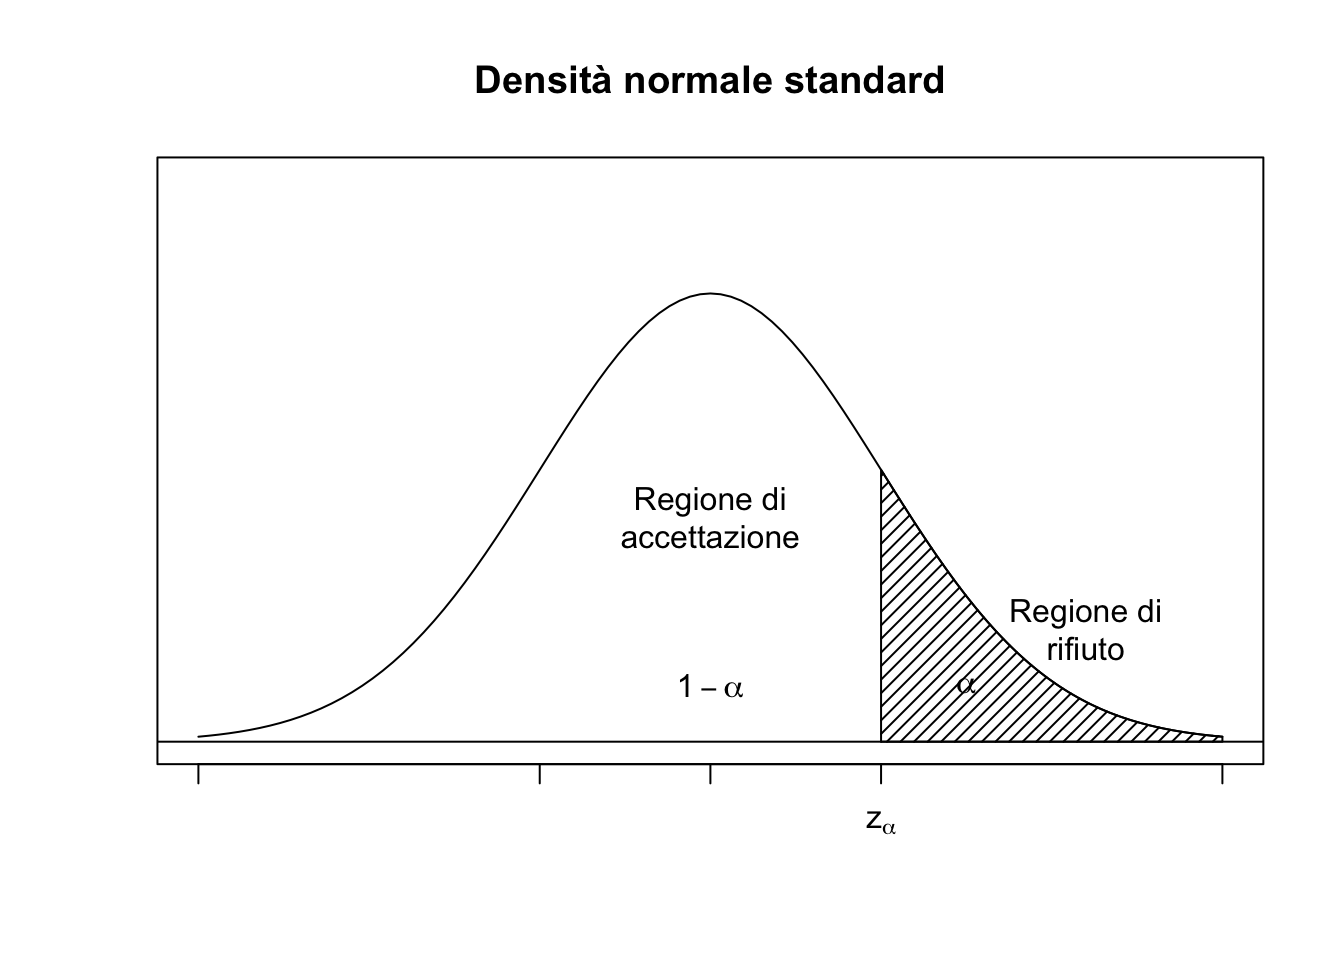
\includegraphics{statistics-project_files/figure-latex/verifica-ipotesi-unilaterale-sinistro-1} 

}

\caption{Densità normale standard}\label{fig:verifica-ipotesi-unilaterale-sinistro}
\end{figure}

La seguente funzione effettua il test unilaterale sinistro approssimato.
La funzione prende in input la media e la deviazione standard della
popolazione, la media campionaria e la misura \(\alpha\).

\begin{Shaded}
\begin{Highlighting}[]
\NormalTok{testUnilateraleSinistro <-}\StringTok{ }\ControlFlowTok{function}\NormalTok{(media, deviazioneStandard, mediaCampionaria, n, alpha) \{}
\NormalTok{  zAlpha <-}\StringTok{ }\KeywordTok{qnorm}\NormalTok{(}\DecValTok{1} \OperatorTok{-}\StringTok{ }\NormalTok{alpha, }\DataTypeTok{mean =} \DecValTok{0}\NormalTok{, }\DataTypeTok{sd =} \DecValTok{1}\NormalTok{)}
\NormalTok{  valore <-}\StringTok{ }\NormalTok{(mediaCampionaria }\OperatorTok{-}\StringTok{ }\NormalTok{media) }\OperatorTok{/}\StringTok{ }\NormalTok{(deviazioneStandard }\OperatorTok{/}\StringTok{ }\KeywordTok{sqrt}\NormalTok{(n))}
\NormalTok{  valore }\OperatorTok{<}\StringTok{ }\NormalTok{zAlpha}
\NormalTok{\}}
\end{Highlighting}
\end{Shaded}

Il seguente codice effettua il test unilaterale sinistro sul valore
medio utilizzando un campione che si ritiene estratto da una popolazione
geometrica di parametro \(p = 0.4\). Vengono quindi calcolati il valore
atteso e la deviazione standard della popolazione e viene poi invocata
la precedente funzione per ottenere il risultato del test.

\begin{Shaded}
\begin{Highlighting}[]
\NormalTok{p <-}\StringTok{ }\FloatTok{0.4}
\NormalTok{media <-}\StringTok{ }\DecValTok{1} \OperatorTok{/}\StringTok{ }\NormalTok{p}
\NormalTok{varianza <-}\StringTok{ }\NormalTok{(}\DecValTok{1} \OperatorTok{-}\StringTok{ }\NormalTok{p) }\OperatorTok{/}\StringTok{ }\NormalTok{p}\OperatorTok{^}\DecValTok{2}
\NormalTok{deviazioneStandard <-}\StringTok{ }\KeywordTok{sqrt}\NormalTok{(varianza)}

\CommentTok{#campione <- rgeom(100, prob = 0.7) + 1}
\NormalTok{campione <-}\StringTok{ }\KeywordTok{c}\NormalTok{(}\DecValTok{2}\NormalTok{, }\DecValTok{2}\NormalTok{, }\DecValTok{1}\NormalTok{, }\DecValTok{1}\NormalTok{, }\DecValTok{3}\NormalTok{, }\DecValTok{1}\NormalTok{, }\DecValTok{2}\NormalTok{, }\DecValTok{1}\NormalTok{, }\DecValTok{1}\NormalTok{, }\DecValTok{2}\NormalTok{, }\DecValTok{3}\NormalTok{, }\DecValTok{1}\NormalTok{, }\DecValTok{1}\NormalTok{, }\DecValTok{1}\NormalTok{, }\DecValTok{3}\NormalTok{, }\DecValTok{2}\NormalTok{, }\DecValTok{2}\NormalTok{, }\DecValTok{1}\NormalTok{, }\DecValTok{1}\NormalTok{, }\DecValTok{2}\NormalTok{, }
              \DecValTok{2}\NormalTok{, }\DecValTok{2}\NormalTok{, }\DecValTok{1}\NormalTok{, }\DecValTok{1}\NormalTok{, }\DecValTok{1}\NormalTok{, }\DecValTok{2}\NormalTok{, }\DecValTok{1}\NormalTok{, }\DecValTok{2}\NormalTok{, }\DecValTok{1}\NormalTok{, }\DecValTok{1}\NormalTok{, }\DecValTok{2}\NormalTok{, }\DecValTok{1}\NormalTok{, }\DecValTok{1}\NormalTok{, }\DecValTok{1}\NormalTok{, }\DecValTok{1}\NormalTok{, }\DecValTok{1}\NormalTok{, }\DecValTok{1}\NormalTok{, }\DecValTok{1}\NormalTok{, }\DecValTok{1}\NormalTok{, }\DecValTok{1}\NormalTok{, }
              \DecValTok{2}\NormalTok{, }\DecValTok{1}\NormalTok{, }\DecValTok{2}\NormalTok{, }\DecValTok{1}\NormalTok{, }\DecValTok{1}\NormalTok{, }\DecValTok{1}\NormalTok{, }\DecValTok{1}\NormalTok{, }\DecValTok{1}\NormalTok{, }\DecValTok{2}\NormalTok{, }\DecValTok{2}\NormalTok{, }\DecValTok{1}\NormalTok{, }\DecValTok{1}\NormalTok{, }\DecValTok{1}\NormalTok{, }\DecValTok{2}\NormalTok{, }\DecValTok{1}\NormalTok{, }\DecValTok{1}\NormalTok{, }\DecValTok{1}\NormalTok{, }\DecValTok{1}\NormalTok{, }\DecValTok{1}\NormalTok{, }\DecValTok{1}\NormalTok{, }
              \DecValTok{1}\NormalTok{, }\DecValTok{1}\NormalTok{, }\DecValTok{1}\NormalTok{, }\DecValTok{1}\NormalTok{, }\DecValTok{3}\NormalTok{, }\DecValTok{1}\NormalTok{, }\DecValTok{1}\NormalTok{, }\DecValTok{3}\NormalTok{, }\DecValTok{1}\NormalTok{, }\DecValTok{1}\NormalTok{, }\DecValTok{1}\NormalTok{, }\DecValTok{1}\NormalTok{, }\DecValTok{1}\NormalTok{, }\DecValTok{1}\NormalTok{, }\DecValTok{2}\NormalTok{, }\DecValTok{2}\NormalTok{, }\DecValTok{1}\NormalTok{, }\DecValTok{1}\NormalTok{, }\DecValTok{1}\NormalTok{, }\DecValTok{1}\NormalTok{, }
              \DecValTok{2}\NormalTok{, }\DecValTok{3}\NormalTok{, }\DecValTok{2}\NormalTok{, }\DecValTok{1}\NormalTok{, }\DecValTok{1}\NormalTok{, }\DecValTok{1}\NormalTok{, }\DecValTok{1}\NormalTok{, }\DecValTok{1}\NormalTok{, }\DecValTok{1}\NormalTok{, }\DecValTok{1}\NormalTok{, }\DecValTok{1}\NormalTok{, }\DecValTok{2}\NormalTok{, }\DecValTok{1}\NormalTok{, }\DecValTok{1}\NormalTok{, }\DecValTok{3}\NormalTok{, }\DecValTok{1}\NormalTok{, }\DecValTok{1}\NormalTok{, }\DecValTok{1}\NormalTok{, }\DecValTok{1}\NormalTok{, }\DecValTok{2}\NormalTok{)}

\NormalTok{esito <-}\StringTok{ }\KeywordTok{testUnilateraleSinistro}\NormalTok{(}\DataTypeTok{media =}\NormalTok{ media, }
                                 \DataTypeTok{deviazioneStandard =}\NormalTok{ deviazioneStandard, }
                                 \DataTypeTok{mediaCampionaria =} \KeywordTok{mean}\NormalTok{(campione), }
                                 \DataTypeTok{n =} \KeywordTok{length}\NormalTok{(campione), }
                                 \DataTypeTok{alpha =} \FloatTok{0.05}\NormalTok{)}
\end{Highlighting}
\end{Shaded}

Il test da esito positivo.

\section{Test unilaterale destro
approssimato}\label{test-unilaterale-destro-approssimato}

Se \((x_1,\dots,x_n)\) è un campione osservato di ampiezza \(n\)
estratto da una popolazione geometrica con varianza nota \(\sigma^2\) e
se consideriamo le ipotesi:

\[H_0 : \mu \ge \mu_0 \quad H_1 : \mu < \mu_0\] allora il test
unilaterale destro \(\Phi\) di misura \(\alpha\) per le ipotesi è:

\emph{Accettiamo l'ipotesi \(H_0\) se}
\[\frac{\overline x - \mu_0}{\sigma / \sqrt{n}} > - z_{\alpha}\]

\emph{Rifiutiamo l'ipotesi \(H_0\) se}
\[\frac{\overline x - \mu_0}{\sigma / \sqrt{n}} < -z_{\alpha}\]

dove \(-z_{\alpha}\) è tale che: \[P(Z < -z_{\alpha}) = \alpha\]

\begin{figure}

{\centering 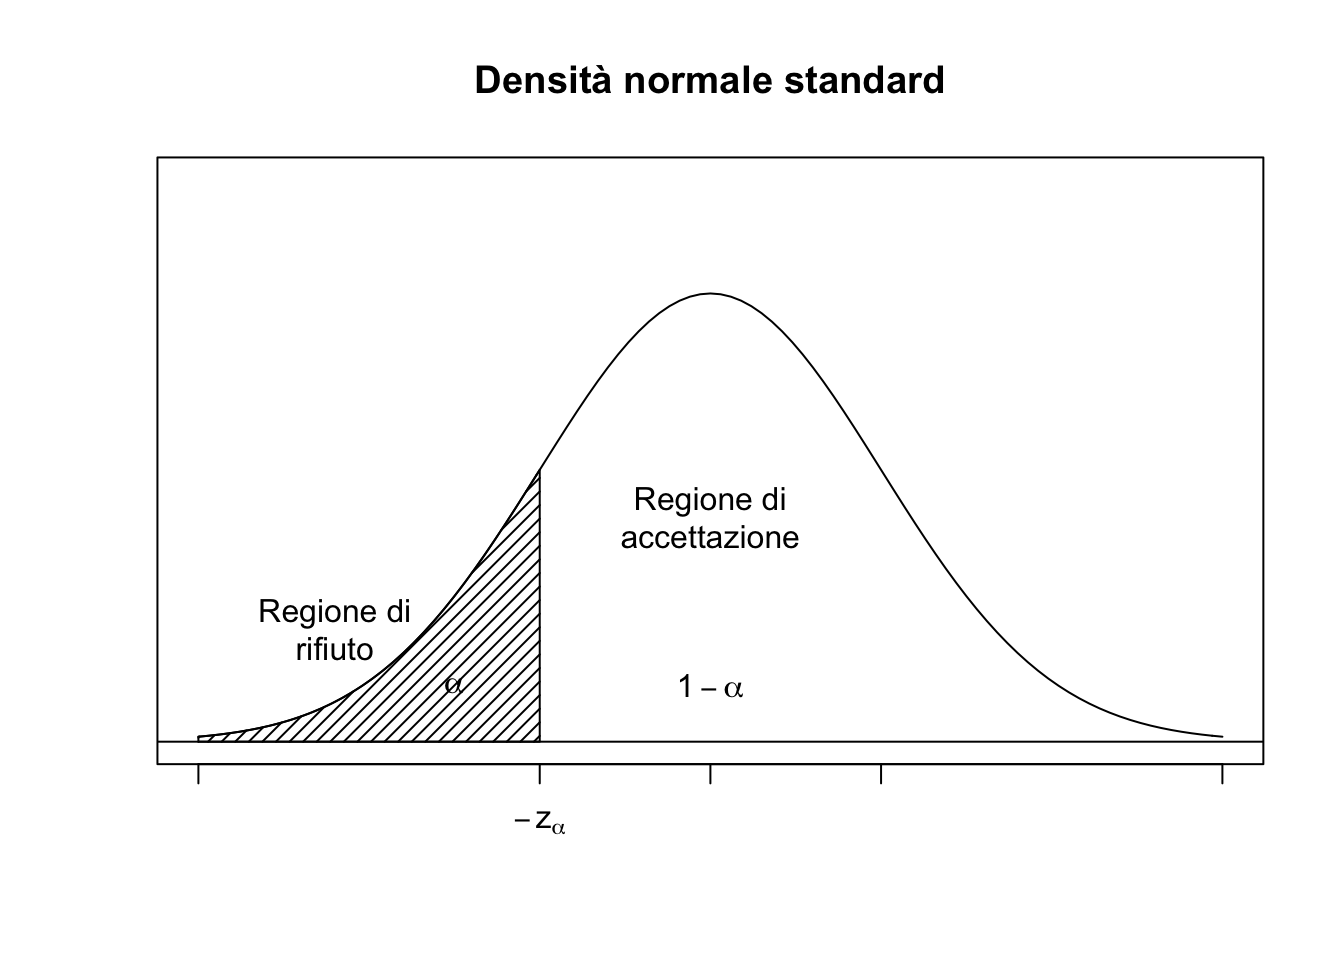
\includegraphics{statistics-project_files/figure-latex/verifica-ipotesi-unilaterale-destro-1} 

}

\caption{Densità normale standard}\label{fig:verifica-ipotesi-unilaterale-destro}
\end{figure}

La seguente funzione effettua il test unilaterale sinistro approssimato.
La funzione prende in input la media e la deviazione standard della
popolazione, la media campionaria e la misura \(\alpha\).

\begin{Shaded}
\begin{Highlighting}[]
\NormalTok{testUnilateraleDestro <-}\StringTok{ }\ControlFlowTok{function}\NormalTok{(media, deviazioneStandard, mediaCampionaria, n, alpha) \{}
\NormalTok{  menoAlpha <-}\StringTok{ }\KeywordTok{qnorm}\NormalTok{(alpha, }\DataTypeTok{mean =} \DecValTok{0}\NormalTok{, }\DataTypeTok{sd =} \DecValTok{1}\NormalTok{)}
\NormalTok{  valore <-}\StringTok{ }\NormalTok{(mediaCampionaria }\OperatorTok{-}\StringTok{ }\NormalTok{media) }\OperatorTok{/}\StringTok{ }\NormalTok{(deviazioneStandard }\OperatorTok{/}\StringTok{ }\KeywordTok{sqrt}\NormalTok{(n))}
\NormalTok{  valore }\OperatorTok{>}\StringTok{ }\NormalTok{menoAlpha}
\NormalTok{\}}
\end{Highlighting}
\end{Shaded}

Il seguente codice effettua il test unilaterale destro sul valore medio
utilizzando un campione che si ritiene estratto da una popolazione
geometrica di parametro \(p = 0.4\). Vengono quindi calcolati il valore
atteso e la deviazione standard della popolazione e viene poi invocata
la precedente funzione per ottenere il risultato del test.

\begin{Shaded}
\begin{Highlighting}[]
\NormalTok{p <-}\StringTok{ }\FloatTok{0.4}
\NormalTok{media <-}\StringTok{ }\DecValTok{1} \OperatorTok{/}\StringTok{ }\NormalTok{p}
\NormalTok{varianza <-}\StringTok{ }\NormalTok{(}\DecValTok{1} \OperatorTok{-}\StringTok{ }\NormalTok{p) }\OperatorTok{/}\StringTok{ }\NormalTok{p}\OperatorTok{^}\DecValTok{2}
\NormalTok{deviazioneStandard <-}\StringTok{ }\KeywordTok{sqrt}\NormalTok{(varianza)}

\CommentTok{#campione <- rgeom(100, prob = 0.7) + 1}
\NormalTok{campione <-}\StringTok{ }\KeywordTok{c}\NormalTok{(}\DecValTok{2}\NormalTok{, }\DecValTok{2}\NormalTok{, }\DecValTok{1}\NormalTok{, }\DecValTok{1}\NormalTok{, }\DecValTok{3}\NormalTok{, }\DecValTok{1}\NormalTok{, }\DecValTok{2}\NormalTok{, }\DecValTok{1}\NormalTok{, }\DecValTok{1}\NormalTok{, }\DecValTok{2}\NormalTok{, }\DecValTok{3}\NormalTok{, }\DecValTok{1}\NormalTok{, }\DecValTok{1}\NormalTok{, }\DecValTok{1}\NormalTok{, }\DecValTok{3}\NormalTok{, }\DecValTok{2}\NormalTok{, }\DecValTok{2}\NormalTok{, }\DecValTok{1}\NormalTok{, }\DecValTok{1}\NormalTok{, }\DecValTok{2}\NormalTok{, }
              \DecValTok{2}\NormalTok{, }\DecValTok{2}\NormalTok{, }\DecValTok{1}\NormalTok{, }\DecValTok{1}\NormalTok{, }\DecValTok{1}\NormalTok{, }\DecValTok{2}\NormalTok{, }\DecValTok{1}\NormalTok{, }\DecValTok{2}\NormalTok{, }\DecValTok{1}\NormalTok{, }\DecValTok{1}\NormalTok{, }\DecValTok{2}\NormalTok{, }\DecValTok{1}\NormalTok{, }\DecValTok{1}\NormalTok{, }\DecValTok{1}\NormalTok{, }\DecValTok{1}\NormalTok{, }\DecValTok{1}\NormalTok{, }\DecValTok{1}\NormalTok{, }\DecValTok{1}\NormalTok{, }\DecValTok{1}\NormalTok{, }\DecValTok{1}\NormalTok{, }
              \DecValTok{2}\NormalTok{, }\DecValTok{1}\NormalTok{, }\DecValTok{2}\NormalTok{, }\DecValTok{1}\NormalTok{, }\DecValTok{1}\NormalTok{, }\DecValTok{1}\NormalTok{, }\DecValTok{1}\NormalTok{, }\DecValTok{1}\NormalTok{, }\DecValTok{2}\NormalTok{, }\DecValTok{2}\NormalTok{, }\DecValTok{1}\NormalTok{, }\DecValTok{1}\NormalTok{, }\DecValTok{1}\NormalTok{, }\DecValTok{2}\NormalTok{, }\DecValTok{1}\NormalTok{, }\DecValTok{1}\NormalTok{, }\DecValTok{1}\NormalTok{, }\DecValTok{1}\NormalTok{, }\DecValTok{1}\NormalTok{, }\DecValTok{1}\NormalTok{, }
              \DecValTok{1}\NormalTok{, }\DecValTok{1}\NormalTok{, }\DecValTok{1}\NormalTok{, }\DecValTok{1}\NormalTok{, }\DecValTok{3}\NormalTok{, }\DecValTok{1}\NormalTok{, }\DecValTok{1}\NormalTok{, }\DecValTok{3}\NormalTok{, }\DecValTok{1}\NormalTok{, }\DecValTok{1}\NormalTok{, }\DecValTok{1}\NormalTok{, }\DecValTok{1}\NormalTok{, }\DecValTok{1}\NormalTok{, }\DecValTok{1}\NormalTok{, }\DecValTok{2}\NormalTok{, }\DecValTok{2}\NormalTok{, }\DecValTok{1}\NormalTok{, }\DecValTok{1}\NormalTok{, }\DecValTok{1}\NormalTok{, }\DecValTok{1}\NormalTok{, }
              \DecValTok{2}\NormalTok{, }\DecValTok{3}\NormalTok{, }\DecValTok{2}\NormalTok{, }\DecValTok{1}\NormalTok{, }\DecValTok{1}\NormalTok{, }\DecValTok{1}\NormalTok{, }\DecValTok{1}\NormalTok{, }\DecValTok{1}\NormalTok{, }\DecValTok{1}\NormalTok{, }\DecValTok{1}\NormalTok{, }\DecValTok{1}\NormalTok{, }\DecValTok{2}\NormalTok{, }\DecValTok{1}\NormalTok{, }\DecValTok{1}\NormalTok{, }\DecValTok{3}\NormalTok{, }\DecValTok{1}\NormalTok{, }\DecValTok{1}\NormalTok{, }\DecValTok{1}\NormalTok{, }\DecValTok{1}\NormalTok{, }\DecValTok{2}\NormalTok{)}

\NormalTok{esito <-}\StringTok{ }\KeywordTok{testUnilateraleDestro}\NormalTok{(}\DataTypeTok{media =}\NormalTok{ media, }
                               \DataTypeTok{deviazioneStandard =}\NormalTok{ deviazioneStandard, }
                               \DataTypeTok{mediaCampionaria =} \KeywordTok{mean}\NormalTok{(campione), }
                               \DataTypeTok{n =} \KeywordTok{length}\NormalTok{(campione), }
                               \DataTypeTok{alpha =} \FloatTok{0.05}\NormalTok{)}
\end{Highlighting}
\end{Shaded}

Il test da esito negativo.

\chapter{Criterio del chi-quadrato}\label{criterio-del-chi-quadrato}

Il criterio del chi-quadrato è un test di verifica delle ipotesi che
consente di verificare se le frequenze dei valori osservati si adattano
alle frequenze teoriche (probabilità) di una data distribuzione di
probabilità e quindi poter dire, con una certa probabilità di errore, se
il campione proviene dalla fissata distribuzione di probabilità.

Consideriamo una popolazione descritta da una variabile aleatoria \(X\)
e avente una distribuzione di probabilità \(F_X(x)\) con \(k\) parametri
non noti da stimare. I parametri non noti possono essere stimati
utilizzando il campione.

Il test di misura \(\alpha\) consiste del verificare l'ipotesi nulla:

\emph{\(H_0\) : \(X\) ha una funzione di distribuzione \(F_X(x)\)}

o l'ipotesi alternativa:

\emph{\(H_1\) : \(X\) non ha una funzione di distribuzione \(F_X(x)\)}

La misura \(\alpha\) è la probabilità di rifiutare l'ipotesi nulla.

Il test consiste nel suddividere l'insieme dei valori che può assumere
la variabile aleatoria \(X\) in \(r\) sottoinsiemi \(I_1,...,I_r\) e
calcolare le probabilità che la variabile aleatoria assuma un valore
appartenente all'\(i\)-esimo sottoinsieme \(p_i = P(X \in I_i)\) per
\(i=1,...,r\)

Preso un campione \(x_1,...x_n\) si calcolano le frequenze assolute
\(n_1,...,n_r\) con cui con i valori osservati si distribuiscono nei
sottoinsiemi \(I_1,...,I_r\)

Si calcola il valore chi-quadrato
\[\chi^2 = \sum_{i=1}^{r}\left(\frac{n_i - np_i}{\sqrt{np_i}}\right)^2\]
pari alla somma dei quadrati degli scarti tra le frequenze teoriche e
quelle osservate pesati sulle frequenze teoriche.

E si considera la statistica

\[Q = \sum_{i=1}^{r}\left(\frac{N_i - np_i}{\sqrt{np_i}}\right)^2\] dove
\(N_i\) è la variabile aleatoria che descrive il numero di elementi del
campione che appartengono all'intervallo \(i\)-esimo.

Se la variabile aleatoria \(X\) ha una funzione di distribuzione
\(F_X(x)\) con \(k\) parametri non noti, allora per \(n\)
sufficientemente grande la variabile aleatoria \(Q\) converge in
distribuzione alla variabile chi-quadrato con \(r-k-1\) gradi di
libertà.\\
Il significato dei gradi di libertà è il seguente: se \(r\) viene
sottratto \(1\) perché se conosciamo \(r-1\) probabilità possiamo
calcolare l'r-esima invece \(k\) indica il numero di parametri non noti
sostituiti da stime.

Il test del chi-quadrato di misura \(\alpha\) per le ipotesi è:

\emph{Accettiamo l'ipotesi \(H_0\) se}

\[\chi^2_{1-\frac{\alpha}{2},r-k-1} < \chi^2 < \chi^2_{\frac{\alpha}{2},r-k-1}\]
\emph{Rifiutiamo l'ipotesi \(H_0\) se}

\[\chi^2 > \chi^2_{\frac{\alpha}{2},r-k-1} \quad \text{oppure} \quad \chi^2 < \chi^2_{1-\frac{\alpha}{2},r-k-1}\]

Dove i valori
\(\chi^2_{\frac{\alpha}{2},r-k-1} \quad \text{e} \quad \chi^2_{1 - \frac{\alpha}{2},r-k-1}\)
sono tali che

\[P\left(Q < \chi^2_{1 -\frac{\alpha}{2},r-k-1} \right) \backsimeq \alpha / 2 \quad \text{e} \quad P\left(Q > \chi^2_{\frac{\alpha}{2},r-k-1} \right) \backsimeq  \alpha / 2\]

Il test funziona se ogni classe contiene in media almeno 5 elementi.

In figura \ref{fig:chi-quadrato} è rappresentata una densità
chi-quadrato e sono mostrate le regioni di rifiuto e di accettazione.

\begin{figure}

{\centering 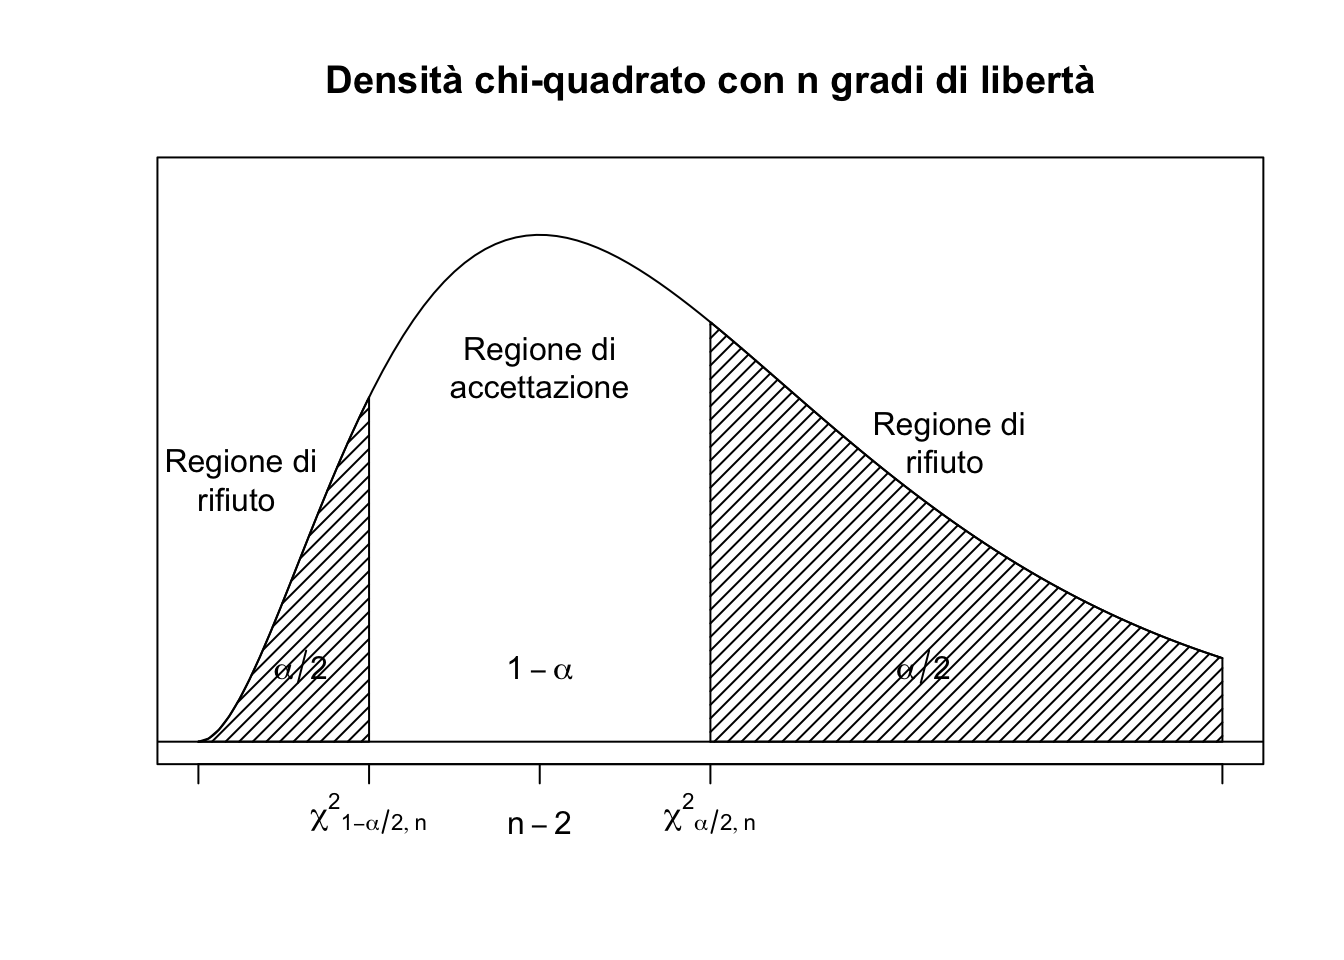
\includegraphics{statistics-project_files/figure-latex/chi-quadrato-1} 

}

\caption{Densità chi-quadrato con n gradi di libertà}\label{fig:chi-quadrato}
\end{figure}

\section{Test per la distribuzione
geometrica}\label{test-per-la-distribuzione-geometrica}

In questo paragrafo verrà effettuato il test del chi-quadrato di misura
\(\alpha = 0.01\) su un campione per verificare la provenienza da una
distribuzione geometrica.

Consideriamo il seguente campione

\begin{Shaded}
\begin{Highlighting}[]
\NormalTok{campione <-}\StringTok{ }\KeywordTok{c}\NormalTok{(}\DecValTok{2}\NormalTok{, }\DecValTok{1}\NormalTok{, }\DecValTok{2}\NormalTok{, }\DecValTok{1}\NormalTok{, }\DecValTok{1}\NormalTok{, }\DecValTok{1}\NormalTok{, }\DecValTok{6}\NormalTok{, }\DecValTok{1}\NormalTok{, }\DecValTok{1}\NormalTok{, }\DecValTok{2}\NormalTok{, }\DecValTok{1}\NormalTok{, }\DecValTok{1}\NormalTok{, }\DecValTok{1}\NormalTok{, }\DecValTok{2}\NormalTok{, }\DecValTok{1}\NormalTok{, }\DecValTok{2}\NormalTok{, }\DecValTok{2}\NormalTok{, }\DecValTok{3}\NormalTok{, }\DecValTok{1}\NormalTok{, }\DecValTok{1}\NormalTok{, }
              \DecValTok{2}\NormalTok{, }\DecValTok{4}\NormalTok{, }\DecValTok{1}\NormalTok{, }\DecValTok{3}\NormalTok{, }\DecValTok{1}\NormalTok{, }\DecValTok{1}\NormalTok{, }\DecValTok{2}\NormalTok{, }\DecValTok{2}\NormalTok{, }\DecValTok{1}\NormalTok{, }\DecValTok{4}\NormalTok{, }\DecValTok{4}\NormalTok{, }\DecValTok{1}\NormalTok{, }\DecValTok{3}\NormalTok{, }\DecValTok{4}\NormalTok{, }\DecValTok{2}\NormalTok{, }\DecValTok{2}\NormalTok{, }\DecValTok{2}\NormalTok{, }\DecValTok{3}\NormalTok{, }\DecValTok{1}\NormalTok{, }\DecValTok{3}\NormalTok{, }
              \DecValTok{1}\NormalTok{, }\DecValTok{1}\NormalTok{, }\DecValTok{1}\NormalTok{, }\DecValTok{1}\NormalTok{, }\DecValTok{2}\NormalTok{, }\DecValTok{3}\NormalTok{, }\DecValTok{1}\NormalTok{, }\DecValTok{1}\NormalTok{, }\DecValTok{1}\NormalTok{, }\DecValTok{1}\NormalTok{, }\DecValTok{1}\NormalTok{, }\DecValTok{1}\NormalTok{, }\DecValTok{1}\NormalTok{, }\DecValTok{1}\NormalTok{, }\DecValTok{4}\NormalTok{, }\DecValTok{1}\NormalTok{, }\DecValTok{1}\NormalTok{, }\DecValTok{2}\NormalTok{, }\DecValTok{1}\NormalTok{, }\DecValTok{1}\NormalTok{, }
              \DecValTok{2}\NormalTok{, }\DecValTok{1}\NormalTok{, }\DecValTok{1}\NormalTok{, }\DecValTok{1}\NormalTok{, }\DecValTok{1}\NormalTok{, }\DecValTok{4}\NormalTok{, }\DecValTok{1}\NormalTok{, }\DecValTok{1}\NormalTok{, }\DecValTok{2}\NormalTok{, }\DecValTok{3}\NormalTok{, }\DecValTok{2}\NormalTok{, }\DecValTok{1}\NormalTok{, }\DecValTok{1}\NormalTok{, }\DecValTok{2}\NormalTok{, }\DecValTok{1}\NormalTok{, }\DecValTok{1}\NormalTok{, }\DecValTok{2}\NormalTok{, }\DecValTok{4}\NormalTok{, }\DecValTok{2}\NormalTok{, }\DecValTok{3}\NormalTok{, }
              \DecValTok{1}\NormalTok{, }\DecValTok{1}\NormalTok{, }\DecValTok{1}\NormalTok{, }\DecValTok{1}\NormalTok{, }\DecValTok{2}\NormalTok{, }\DecValTok{1}\NormalTok{, }\DecValTok{3}\NormalTok{, }\DecValTok{1}\NormalTok{, }\DecValTok{3}\NormalTok{, }\DecValTok{6}\NormalTok{, }\DecValTok{5}\NormalTok{, }\DecValTok{1}\NormalTok{, }\DecValTok{1}\NormalTok{, }\DecValTok{1}\NormalTok{, }\DecValTok{1}\NormalTok{, }\DecValTok{1}\NormalTok{, }\DecValTok{2}\NormalTok{, }\DecValTok{2}\NormalTok{, }\DecValTok{1}\NormalTok{, }\DecValTok{1}\NormalTok{)}
\end{Highlighting}
\end{Shaded}

Con il seguente codice viene stimato il parametro non noto della
distribuzione geometrica tramite inferenza sul campione.

\begin{Shaded}
\begin{Highlighting}[]
\NormalTok{stima.p <-}\StringTok{ }\DecValTok{1} \OperatorTok{/}\StringTok{ }\KeywordTok{mean}\NormalTok{(campione) }
\end{Highlighting}
\end{Shaded}

Nel seguente codice consideriamo 4 sottoinsiemi dei valori che può
assumere una variabile aleatoria distribuita in modo geometrico. E per
ogni sottoinsieme calcoliamo la probabilità che il valore della
variabile aleatoria appartenga all'insieme.

\begin{Shaded}
\begin{Highlighting}[]
\NormalTok{r =}\StringTok{ }\DecValTok{4}
\NormalTok{p <-}\StringTok{ }\KeywordTok{numeric}\NormalTok{(r)}
\NormalTok{p[}\DecValTok{1}\NormalTok{] <-}\StringTok{ }\KeywordTok{dgeom}\NormalTok{(}\DecValTok{0}\NormalTok{, }\DataTypeTok{prob =}\NormalTok{ stima.p) }\CommentTok{# \{1\}}
\NormalTok{p[}\DecValTok{2}\NormalTok{] <-}\StringTok{ }\KeywordTok{dgeom}\NormalTok{(}\DecValTok{1}\NormalTok{, }\DataTypeTok{prob =}\NormalTok{ stima.p) }\CommentTok{# \{2\}}
\NormalTok{p[}\DecValTok{3}\NormalTok{] <-}\StringTok{ }\KeywordTok{dgeom}\NormalTok{(}\DecValTok{2}\NormalTok{, }\DataTypeTok{prob =}\NormalTok{ stima.p) }\CommentTok{# \{3\}}
\NormalTok{p[}\DecValTok{4}\NormalTok{] <-}\StringTok{ }\KeywordTok{pgeom}\NormalTok{(}\DecValTok{2}\NormalTok{, }\DataTypeTok{prob =}\NormalTok{ stima.p, }\DataTypeTok{lower.tail =} \OtherTok{FALSE}\NormalTok{) }\CommentTok{# [4, +infinity)}
\end{Highlighting}
\end{Shaded}

É possibile effettuare il test del chi-quadrato se ogni classe contiene
in media almeno 5 elementi. Il mimino numero di elementi contenuti in
media in una classe è calcolato con il seguente codice

\begin{Shaded}
\begin{Highlighting}[]
\NormalTok{n <-}\StringTok{ }\KeywordTok{length}\NormalTok{(campione)}
\NormalTok{minimo <-}\StringTok{ }\KeywordTok{min}\NormalTok{(n }\OperatorTok{*}\StringTok{ }\NormalTok{p[}\DecValTok{1}\NormalTok{], n }\OperatorTok{*}\StringTok{ }\NormalTok{p[}\DecValTok{2}\NormalTok{], n }\OperatorTok{*}\StringTok{ }\NormalTok{p[}\DecValTok{3}\NormalTok{], n }\OperatorTok{*}\StringTok{ }\NormalTok{p[}\DecValTok{4}\NormalTok{])}
\end{Highlighting}
\end{Shaded}

ed il risultato è 8.4144125 di conseguenza è possibile effettuare il
test.

Il seguente codice calcola le frequenze dei valori osservati per ogni
intervallo.

\begin{Shaded}
\begin{Highlighting}[]
\NormalTok{nint <-}\StringTok{ }\KeywordTok{numeric}\NormalTok{(}\DecValTok{4}\NormalTok{)}
\NormalTok{nint[}\DecValTok{1}\NormalTok{] <-}\StringTok{ }\KeywordTok{length}\NormalTok{(}\KeywordTok{which}\NormalTok{(campione }\OperatorTok{==}\StringTok{ }\DecValTok{1}\NormalTok{))}
\NormalTok{nint[}\DecValTok{2}\NormalTok{] <-}\StringTok{ }\KeywordTok{length}\NormalTok{(}\KeywordTok{which}\NormalTok{(campione }\OperatorTok{==}\StringTok{ }\DecValTok{2}\NormalTok{))}
\NormalTok{nint[}\DecValTok{3}\NormalTok{] <-}\StringTok{ }\KeywordTok{length}\NormalTok{(}\KeywordTok{which}\NormalTok{(campione }\OperatorTok{==}\StringTok{ }\DecValTok{3}\NormalTok{))}
\NormalTok{nint[}\DecValTok{4}\NormalTok{] <-}\StringTok{ }\KeywordTok{length}\NormalTok{(}\KeywordTok{which}\NormalTok{(campione }\OperatorTok{>}\StringTok{ }\DecValTok{3}\NormalTok{))}
\end{Highlighting}
\end{Shaded}

Il seguente codice calcola il valore \(\chi^2\)

\begin{Shaded}
\begin{Highlighting}[]
\NormalTok{chi2 <-}\StringTok{ }\KeywordTok{sum}\NormalTok{(((nint }\OperatorTok{-}\StringTok{ }\NormalTok{n }\OperatorTok{*}\StringTok{ }\NormalTok{p) }\OperatorTok{/}\StringTok{ }\KeywordTok{sqrt}\NormalTok{(n }\OperatorTok{*}\StringTok{ }\NormalTok{p)) }\OperatorTok{^}\StringTok{ }\DecValTok{2}\NormalTok{)}
\end{Highlighting}
\end{Shaded}

Il valore di \(\chi^2\) calcolato è 0.4746316

Mentre il seguente codice calcola l'intervallo
\(\left( \chi^2_{1 - \frac{\alpha}{2},r-k-1}, \quad \chi^2_{\frac{\alpha}{2},r-k-1} \right)\)

\begin{Shaded}
\begin{Highlighting}[]
\NormalTok{k <-}\StringTok{ }\DecValTok{1}
\NormalTok{alpha <-}\StringTok{ }\FloatTok{0.01}
\NormalTok{df <-}\StringTok{ }\NormalTok{r }\OperatorTok{-}\StringTok{ }\NormalTok{k }\OperatorTok{-}\StringTok{ }\DecValTok{1}
\NormalTok{valori <-}\StringTok{ }\KeywordTok{c}\NormalTok{(}\KeywordTok{qchisq}\NormalTok{(alpha }\OperatorTok{/}\StringTok{ }\DecValTok{2}\NormalTok{, }\DataTypeTok{df =}\NormalTok{ df), }\KeywordTok{qchisq}\NormalTok{(}\DecValTok{1} \OperatorTok{-}\StringTok{ }\NormalTok{alpha }\OperatorTok{/}\StringTok{ }\DecValTok{2}\NormalTok{, }\DataTypeTok{df =}\NormalTok{df))}
\end{Highlighting}
\end{Shaded}

L'intervallo calcolato è (0.0100251, 10.5966347).

Infine il seguente codice effettua il test del chi-quadrato

\begin{Shaded}
\begin{Highlighting}[]
\NormalTok{esito <-}\StringTok{ }\NormalTok{valori[}\DecValTok{1}\NormalTok{] }\OperatorTok{<}\StringTok{ }\NormalTok{chi2 }\OperatorTok{&&}\StringTok{ }\NormalTok{chi2 }\OperatorTok{<}\StringTok{ }\NormalTok{valori[}\DecValTok{2}\NormalTok{]}
\end{Highlighting}
\end{Shaded}

L'esito ottenuto del test è positivo, di conseguenza possiamo affermare
che il campione proviene da una popolazione descritta da una
distribuzione geometrica.

\bibliography{book.bib,packages.bib}


\end{document}
